%****************************************************
%	CHAPTER 4 - PIPELINE DESIGN
%****************************************************
\chapter{Pipeline Design}
\label{chap:systemDesign}

This chapter's objective is to detail the core design process of this project, a wave parameter extraction pipeline. The fundamental design which needed to be achieved was the extraction of wave parameters from \acs{sar} data. In order to achieve this, 

% \begin{figure}[H]
%     \centering
%     \resizebox{0.9\linewidth}{!}{
\definecolor{c1a1a1a}{RGB}{26,26,26}
\definecolor{c999999}{RGB}{153,153,153}
\definecolor{cff6600}{RGB}{255,102,0}
\definecolor{cb3b3b3}{RGB}{179,179,179}
\definecolor{navy}{RGB}{0,0,128}


\def \globalscale {1.000000}
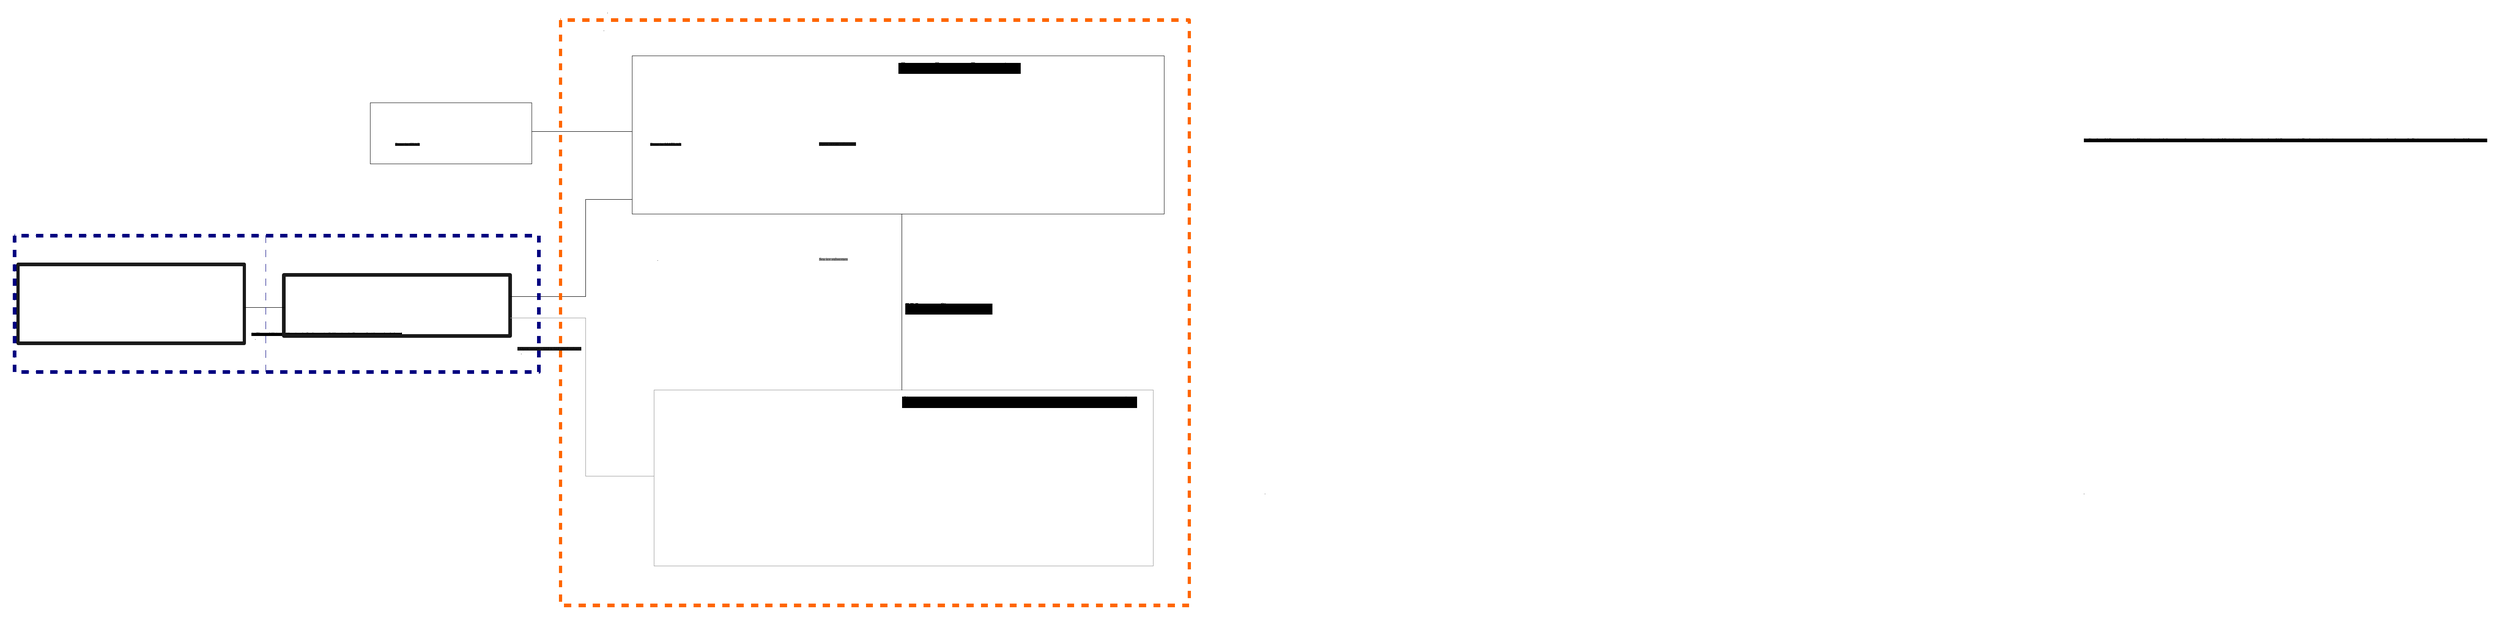
\begin{tikzpicture}[y=1cm, x=1cm, yscale=\globalscale,xscale=\globalscale, inner sep=0pt, outer sep=0pt]
  \path[draw=c1a1a1a,fill=c1a1a1a,fill opacity=0.0,line cap=butt,line
  join=round,line width=0.1cm] (0.2, 22.1) rectangle (6.5, 19.9);
  \node[fill=black,cm={ 0.3,-0.0,-0.0,0.3,(-2.0, 17.6)},anchor=south west]
  (text2) at (8.8, 2.4){};      \node[fill=black,cm={ 0.3,-0.0,-0.0,0.3,(-2.0,
  17.6)},anchor=south west] (text3) at (8.7, 2.5){1. Thermal Noise Calibration
  2. Radiometric Calibration  3. Extract Incidence Angle band};
  \path[draw=c1a1a1a,fill=blue,fill opacity=0.0,draw opacity=1.0,line
  cap=butt,line join=round,line width=0.1cm] (7.6, 21.8) rectangle (13.9, 20.1);
  \node[fill=black,cm={ 0.3,-0.0,-0.0,0.3,(5.4, 17.2)},anchor=south west]
  (text2-9) at (8.8, 2.4){};      \node[fill=c1a1a1a,cm={
  0.3,-0.0,-0.0,0.3,(5.4, 17.2)},anchor=south west] (text3-5) at (8.7, 2.5){-
  Open ocean  - 512 x 512 pixel subsets};      \path[draw=c1a1a1a,fill=blue,fill
  opacity=0.0,draw opacity=1.0,line cap=butt,line join=round,line width=0.0cm]
  (10.0, 26.6) rectangle (14.5, 24.9);      \node[fill=black,cm={
  0.3,-0.0,-0.0,0.3,(7.8, 22.0)},anchor=south west] (text2-9-0) at (8.8, 7.1){};
  \node[fill=c1a1a1a,cm={ 0.3,-0.0,-0.0,0.3,(7.8, 22.1)},anchor=south west]
  (text3-5-9) at (8.7, 6.5){};      \node[fill=c1a1a1a,cm={
  0.3,-0.0,-0.0,0.3,(13.8, 18.9)},anchor=south west] (text3-5-9-5-1) at (8.7,
  6.5){Open ocean subscenes};      \node[fill=c1a1a1a,cm={
  0.3,-0.0,-0.0,0.3,(9.3, 15.7)},anchor=south west] (text3-5-9-5-1-9) at (8.7,
  6.5){};      \node[fill=c1a1a1a,cm={ 0.3,-0.0,-0.0,0.3,(9.1,
  18.9)},anchor=south west] (text3-5-9-5-1-9-0) at (8.7, 6.5){Done in MATLAB};
  \node[fill=c1a1a1a,cm={ 0.3,-0.0,-0.0,0.3,(2.0, 18.9)},anchor=south west]
  (text3-5-9-5-1-9-0-5) at (8.7, 6.5){Done in SNAP};   \node[fill=c999999,cm={
  0.3,-0.0,-0.0,0.3,(13.8, 15.7)},anchor=south west]   (text3-5-9-5-1-2) at
  (8.7, 6.5){Sea ice subscenes};      \path[draw=black,even   odd rule,line
  cap=butt,line join=miter,line width=0.0cm] (6.5, 20.9) -- (7.6,   20.9);
  \path[draw=c1a1a1a,fill=blue,fill opacity=0.0,draw   opacity=1.0,line
  cap=butt,line join=round,line width=0.0cm] (17.3, 27.9)   rectangle (32.1,
  23.5);      \node[fill=black,line width=0.0cm,anchor=south   west] (text6) at
  (24.7, 27.4){Open Ocean Inversion};   \node[fill=black,cm={
  0.3,-0.0,-0.0,0.3,(-0.2, 20.3)},anchor=south west]   (text7) at (57.9, 5.2){1.
  Simulate SAR spectrum ( 2. Use in-situ wind data to   confirm wave direction
  3. Minimise observed vs. simulate SAR spectra  4.   Further minimisation w.r.t
  propogation direction of peak wave  5. Estimate   wave spectrum from SAR
  spectrum};      \path[draw=c999999,fill=blue,fill   opacity=0.0,draw
  opacity=1.0,line cap=butt,line join=round,line width=0.0cm]   (17.9, 18.6)
  rectangle (31.8, 13.7);      \node[fill=black,line   width=0.0cm,anchor=south
  west] (text6-9) at (24.8, 18.1){Sea Ice Inversion   Wave propogation model};
  \node[fill=black,cm={ 0.3,-0.0,-0.0,0.3,(-0.2,   10.5)},anchor=south west]
  (text7-6) at (57.9, 5.2){};   \path[draw=black,even odd rule,line
  cap=butt,line join=miter,line width=0.0cm]   (24.8, 23.5) -- (24.8, 18.6);
  \node[fill=black,line   width=0.0cm,anchor=south west] (text19) at (24.9,
  20.7){Wave Spectrum};   \path[draw=c999999,line cap=butt,line join=miter,line
  width=0.0cm] (13.9,   20.6) -- (14.9, 20.6) -- (16.0, 20.6) -- (16.0, 16.2) --
  (17.9, 16.2);   \path[draw=black,line cap=butt,line join=miter,line
  width=0.0cm] (13.9, 21.2)   -- (16.0, 21.2) -- (16.0, 23.9) -- (17.3, 23.9);
  \path[draw=cff6600,fill=cb3b3b3,fill opacity=0.0,draw opacity=1.0,line
  cap=butt,line join=round,line width=0.1cm,dash pattern=on 0.2cm off 0.2cm]
  (15.3, 28.9) rectangle (32.8, 12.6);      \path[draw=navy,fill=cb3b3b3,fill
  opacity=0.0,draw opacity=1.0,line cap=butt,line join=round,line
  width=0.1cm,dash pattern=on 0.2cm off 0.2cm] (0.1, 22.9) rectangle (14.7,
  19.1);      \path[draw=navy,fill=cb3b3b3,fill opacity=0.0,draw
  opacity=1.0,line cap=butt,line join=round,line width=0.0cm,dash pattern=on
  0.2cm off 0.2cm] (0.1, 22.9) rectangle (7.1, 19.1);   \node[fill=c1a1a1a,cm={
  0.3,-0.0,-0.0,0.3,(26.2, 9.2)},anchor=south west]   (text3-5-9-5-1-4) at (8.7,
  6.5){};      \path[draw=black,even odd rule,line   cap=butt,line
  join=miter,line width=0.0cm] (14.5, 25.8) -- (17.3, 25.8);
\end{tikzpicture}
}
%     \caption{Block Diagram in tex}
%     \label{fig:testPlotBlock}
% \end{figure}

% \begin{figure}[H]
%    \centering
%    %\begin{tabular}{@{}c@{\hspace{.2cm}}c@{}}
%        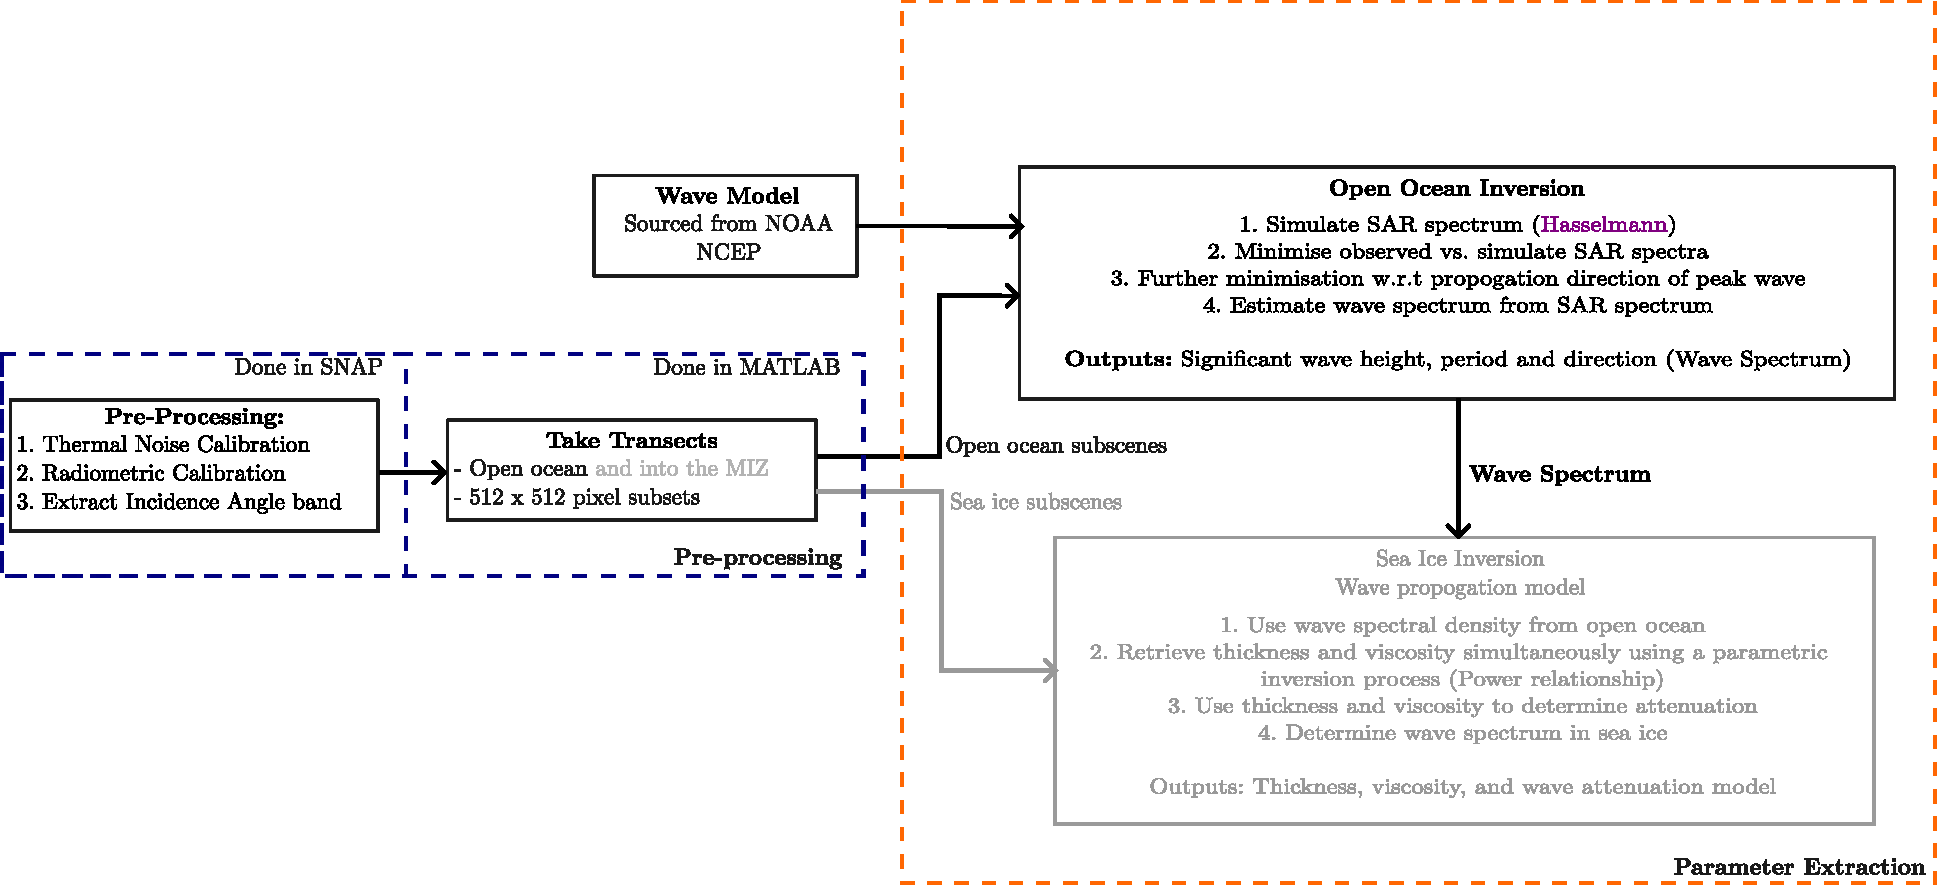
\includegraphics[page=1,width=.9\linewidth]{Figures/PipelineDesign/overall_project.pdf}
%    %\end{tabular}
%  \caption{Test}
%  \label{fig:Test}
% \end{figure}


This chapter begins by providing an overview of the entire pipeline - part of which falls outside of the scope of this project, however, this context is relevant in terms of giving context to the desired results for this project in the context of the broader goals of this pipeline. Each subsequent section will unpack the four main sub-modules within the pipeline in a respective section. Each of these sections will further break down the sub-module into smaller blocks which make up the sub-module. The use of block diagrams allows the process the be understood in terms of the flow of the pipeline, and block diagrams are used throughout this chapter to break down higher-level processes. The variable and function names utilised in this chapter, match those used in the \textsc{Matlab} pipeline.

\section{Overview} \label{sec:systemDesign.overview}

As detailed in xxx, this project required wave parameter extraction for use in a sea ice parameter extraction pipeline. This entire system design is shown as a block diagram in Figure \ref{fig:systemDesign.wholeProject}. It is evident from Figure \ref{fig:systemDesign.wholeProject}, which parts of the \acs{sar} sea ice parameter are relevant to this project. A more detailed block diagram of the wave parameter extraction process is shown in Figure \ref{fig:systemDesign.scope} and within this pipeline, five main functional blocks were identified and are highlighted by five unique colours. [ADD WAVE SPECTRUM GENERATION PIECES]
% Will still change
\begin{figure}[H]
    \centering
    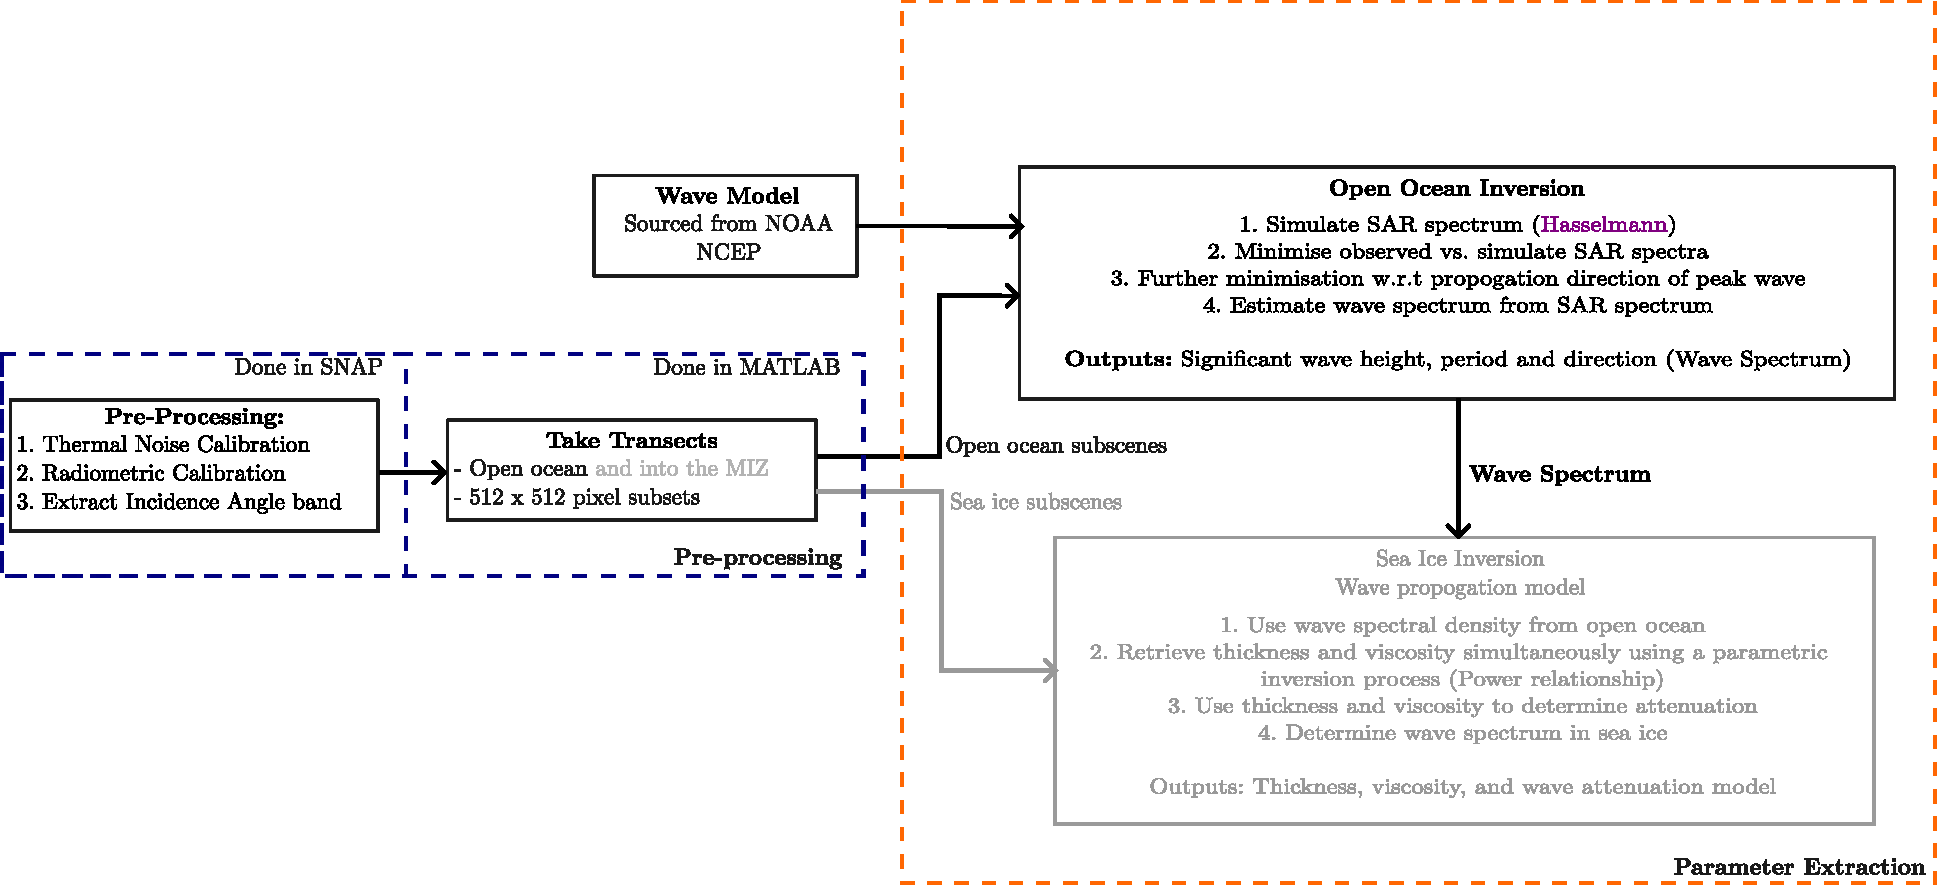
\includegraphics[width=.95\linewidth]{Figures/PipelineDesign/overall_project.pdf}
    \caption{Pipeline system design in the context of the entire parameter extraction process. The scope of this project is shown in black text, with parts of the pipeline outside of the scope, shown in grey.}
    \label{fig:systemDesign.wholeProject}
\end{figure}

% Word better and slim down - ADD DISCUSSION ON WAVE SPECTRUM GENERATION
The five functional blocks were identified as \textsc{pre-processing}, \textsc{metadata extraction}, \textsc{\acs{sar} spectrum calculation}, \textsc{wave spectrum generation}, and \textsc{inversion}. The \textsc{pre-processing} block involves the use of the \ac{snap} Toolbox developed by \ac{esa} as well as \textsc{Matlab}, developed by MathWorks Inc. The \textsc{pre-processing} block reads in a downloaded \acs{sar} Level-1 \ac{grd} data file and outputs a \textsc{Matlab} structure array\footnote{In \textsc{Matlab}, a structure array is a type of data that organises related data into groups. These groups are indexed using an associated field value which can hold any particular data type. More information on structure arrays can be found in the \href{https://www.mathworks.com/help/matlab/ref/struct.html}{\textsc{Matlab} documentation}. The rest of this report will refer to structure arrays simply as structures.} of \lstinline[columns=fixed]{n} equal-sized transects. These equal-sized transects can be input to the \textsc{inversion} block. The output \ac{netcdf} file from \acs{snap} is used to generate views of \acs{sar} data in \textsc{Matlab}, as well as storing the metadata for the \textsc{metadata extraction} block. The \ac{netcdf} file is read by the \textsc{metadata extraction} block and outputs the desired metadata values required for the \textsc{\acs{sar} spectrum calculation} block. The \textsc{\acs{sar} spectrum calculation} block reads in a wave spectrum sourced from \ac{ncep} and generates a \acs{sar} spectrum of the provided wave spectrum. This generated \acs{sar} spectrum is input to the \textsc{inversion} block along with the output of the \textsc{metadata extraction} block. The \textsc{inversion} block outputs the wave parameters from the input pre-processed \acs{sar} data.
% Will still change
\begin{figure}[H]
    \centering
    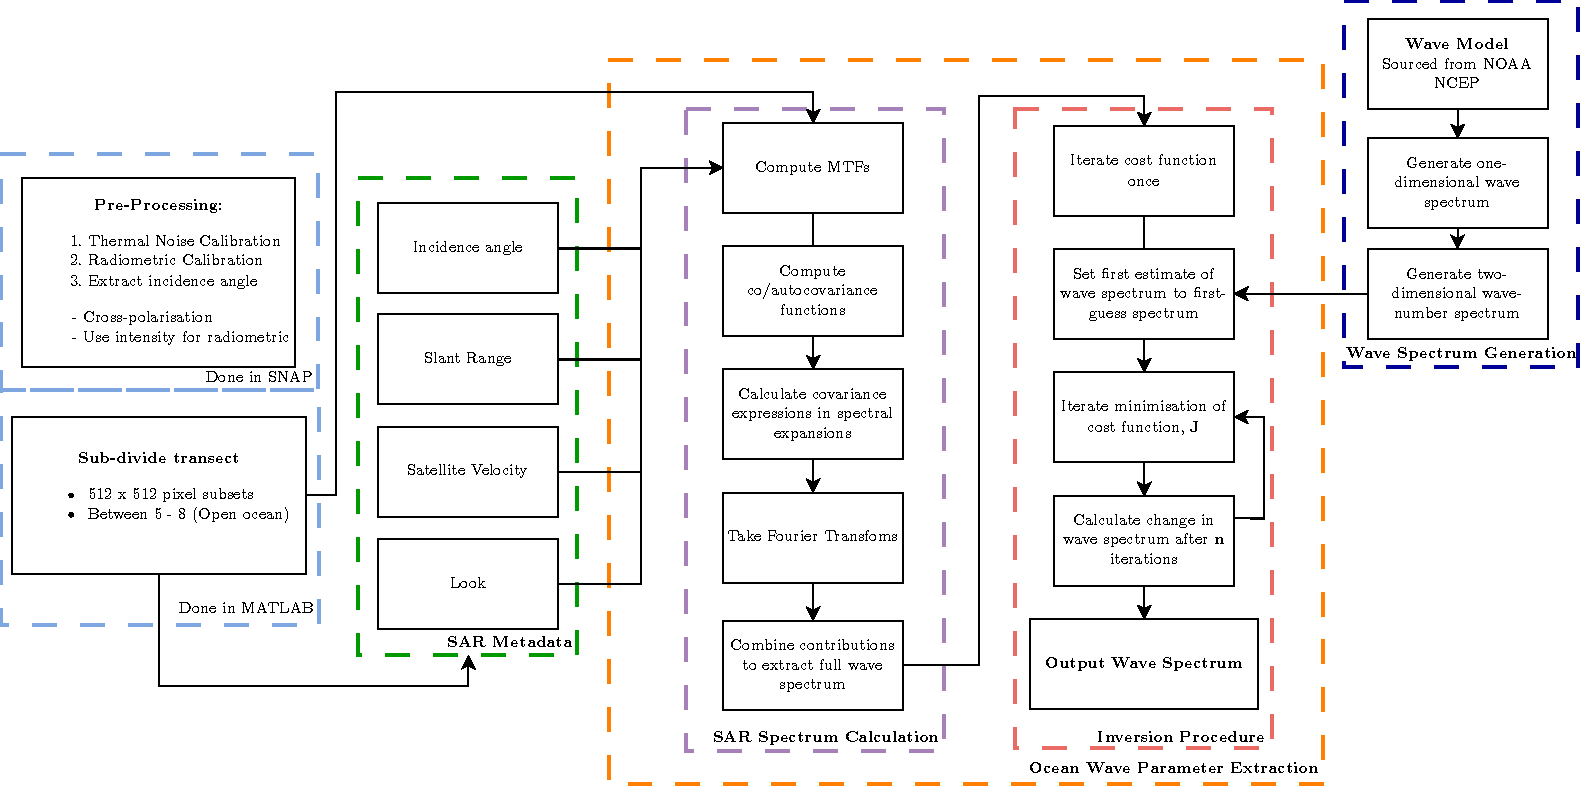
\includegraphics[width=.95\linewidth]{Figures/PipelineDesign/4022_pipeline.pdf}
    \caption{Pipeline system design for the scope of this project broken down further than the entire pipeline shown in Figure \ref{fig:systemDesign.wholeProject}. All the required metadata and external models are shown, along with the part of the process that they are required.}
    \label{fig:systemDesign.scope}
\end{figure}
%====================================================
% PRE-PROCESSING
%====================================================
\section{Pre-processing} \label{sec:systemDesign.preProcessing}


\subsection{Overview} \label{subsec:systemDesign.preProcessing.Overview}

The pre-processing block of the pipeline was designed in a hybrid manner, with part of the pre-processing done in the \ac{snap} toolbox developed by \ac{esa} prior to the use of \textsc{Matlab} tools. The pre-processing block was designed to have an overall function of reading in \ac{s1a} data, apply the desired pre-processing techniques to the \acs{sar} data, and take 512x512 pixel sized transects of this larger \acs{sar} data. The applied pre-processing techniques to calibrate \acs{sar} data for wave parameter extraction were on the recommendation of Giacomo De Carolis and Francesca De Santi of the \acs{irea}, however, discussion around the use of different processing techniques is presented in Chapter \ref{chap:discussion}. The design of this block was designed to keep pre-processing outside of the \textsc{Matlab} environment to a minimum, through the use of external tools. 

The pre-processing block had six notable stages: Thermal noise calibration of \acs{s1a} \acs{grd} data, radiometric calibration of these data, extraction of individual pixel incidence angle, exporting calibrated \acs{grd} data to a usable format for \textsc{Matlab}, reading in the exported data, and taking 512x512 pixel transects of the larger \acs{sar} data. The flow of this block of the pipeline is shown graphically in Figure \ref{fig:systemDesign.preProcessing.blockDiagram}.

\begin{figure}[H]
    \centering
    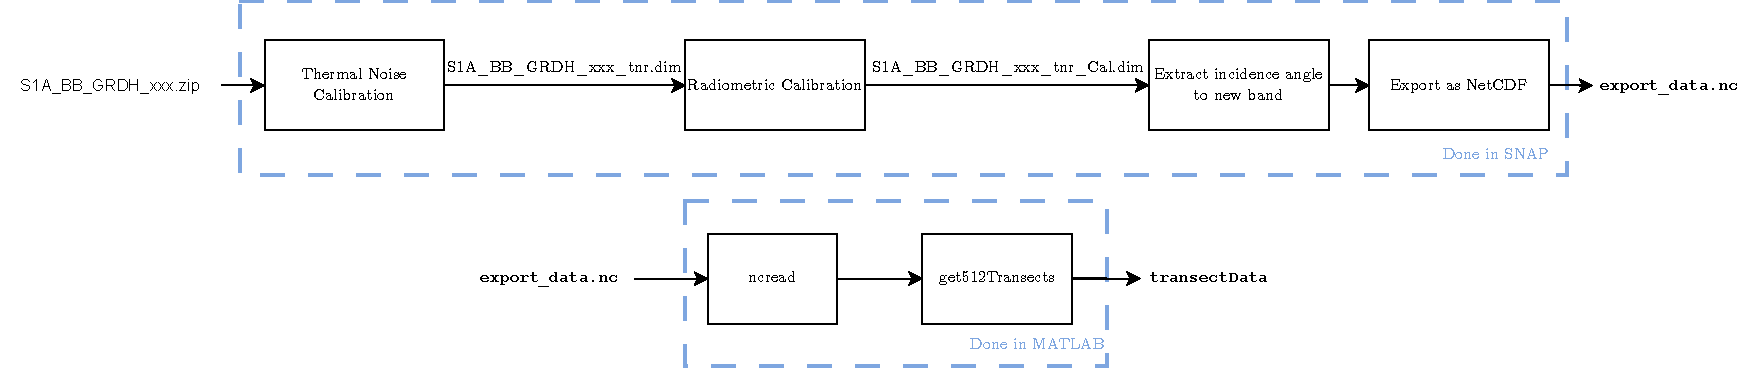
\includegraphics[width=.95\linewidth]{Figures/PipelineDesign/pre_processing.pdf}
    \caption{Block diagram depicting an expanded pre-processing sub-block of Figure \ref{fig:systemDesign.scope}}
    \label{fig:systemDesign.preProcessing.blockDiagram}
\end{figure}

\subsection{Thermal Noise Calibration} \label{subsec:systemDesign.preProcessing.thermalNoise}

After obtaining \acs{grd} \acs{sar} data from \href{scihub.copernicus.eu/dhus/#/home}{Copernicus SciHub}, the first sub-block of the pre-processing block was Thermal Noise Calibration. \acs{s1a} data contains large amounts of thermal noise and as such, \acs{snap} contains a built-in function called \lstinline{S-1 Thermal Noise Removal}. For this block, this function was implemented in \acs{snap} Desktop and is detailed in \href{https://github.com/JNSRYA006/sar-parameter-extraction-pipeline/blob/main/functions/[pipeline.mlx]}{\lstinline{pipeline.mlx}}.

\subsection{Radiometric Calibration} \label{subsec:systemDesign.preProcessing.radiometric}

After removing thermal noise from \acs{grd} \acs{sar} data, the second sub-block of the pre-processing block was Radiometric Calibration. \acs{snap} contains a built-in function called \lstinline{Calibrate} within the \lstinline{Radiometric} block of functions. For this block, this function was implemented in \acs{snap} Desktop and is detailed in \href{https://github.com/JNSRYA006/sar-parameter-extraction-pipeline/blob/main/functions/[pipeline.mlx]}{\lstinline{pipeline.mlx}}.

\subsection{Incidence Angle Extraction} \label{subsec:systemDesign.preProcessing.incidenceAngle}

Due to the fact that the incidence angle varies for each pixel in \acs{sar} data, this exact per-pixel incidence angle is required in order to calculate Equations \ref{eq:hh.rar.Tt_k}, \ref{eq:hh.motion.Tv_k}, which form part of the co and autocovariance functions described in Section \ref{subsec:theory.hasselmann.sarImaging}. In order to achieve this, multiple approaches were investigated. 

Firstly, the metadata file from \acs{s1a} \acs{grd} data was found to contain near and far-look incidence angles. The initial idea to extract individual pixel incidence angle values was to use \textsc{Matlab}'s built-in \lstinline{linspace} function which creates an evenly spaced vector over the range of values. This was an incorrect implementation as the incidence angle is not a linear relation to the latitude and longitude of an image. Furthermore, this method meant that each longitude of the image contained the same incidence angle value, and only the latitude of the image changed.

Secondly, a second type of metadata from \acs{s1a} \acs{grd} data was investigated. This metadata was in the form of a tie-point grid, which provided a 4x4 matrix of incidence angle data, using \lstinline{linspace} on this metadata resulted in a per-pixel incidence angle value which changed in latitude, as well as longitude which is an improvement from the first method.

Finally, tie-point grid data was exported as a band using \acs{snap} Desktop. The way in which this is achieved is detailed in \href{https://github.com/JNSRYA006/sar-parameter-extraction-pipeline/blob/main/functions/[pipeline.mlx]}{\lstinline{pipeline.mlx}}. These data provide a pixel-by-pixel value of the incidence angle on the \acs{s1a} data. Exporting the tie-point grid as a band, allows this band to be imported in \textsc{Matlab} using the \lstinline{ncread} function discussed in Section \ref{subsec:systemDesign.preProcessing.importData}.

In order to decide which method to use, plots of these data were generated over a range of pixel values. Figure \ref{fig:systemDesign.preProcessing.incidence}.

\begin{figure}[H]
    \centering
    \begin{subfigure}{0.48\linewidth}
        \centering
        \resizebox{\linewidth}{!}{% This file was created by matlab2tikz.
%
%The latest updates can be retrieved from
%  http://www.mathworks.com/matlabcentral/fileexchange/22022-matlab2tikz-matlab2tikz
%where you can also make suggestions and rate matlab2tikz.
%
\begin{tikzpicture}

\begin{axis}[%
width=3.97in,
height=3.566in,
at={(0.666in,0.481in)},
scale only axis,
point meta min=31.6384754180908,
point meta max=34.2659797668457,
axis on top,
xmin=0.5,
xmax=4.5,
y dir=reverse,
ymin=0.5,
ymax=4.5,
axis background/.style={fill=white},
colormap={mymap}{[1pt] rgb(0pt)=(0.2422,0.1504,0.6603); rgb(1pt)=(0.2444,0.1534,0.6728); rgb(2pt)=(0.2464,0.1569,0.6847); rgb(3pt)=(0.2484,0.1607,0.6961); rgb(4pt)=(0.2503,0.1648,0.7071); rgb(5pt)=(0.2522,0.1689,0.7179); rgb(6pt)=(0.254,0.1732,0.7286); rgb(7pt)=(0.2558,0.1773,0.7393); rgb(8pt)=(0.2576,0.1814,0.7501); rgb(9pt)=(0.2594,0.1854,0.761); rgb(11pt)=(0.2628,0.1932,0.7828); rgb(12pt)=(0.2645,0.1972,0.7937); rgb(13pt)=(0.2661,0.2011,0.8043); rgb(14pt)=(0.2676,0.2052,0.8148); rgb(15pt)=(0.2691,0.2094,0.8249); rgb(16pt)=(0.2704,0.2138,0.8346); rgb(17pt)=(0.2717,0.2184,0.8439); rgb(18pt)=(0.2729,0.2231,0.8528); rgb(19pt)=(0.274,0.228,0.8612); rgb(20pt)=(0.2749,0.233,0.8692); rgb(21pt)=(0.2758,0.2382,0.8767); rgb(22pt)=(0.2766,0.2435,0.884); rgb(23pt)=(0.2774,0.2489,0.8908); rgb(24pt)=(0.2781,0.2543,0.8973); rgb(25pt)=(0.2788,0.2598,0.9035); rgb(26pt)=(0.2794,0.2653,0.9094); rgb(27pt)=(0.2798,0.2708,0.915); rgb(28pt)=(0.2802,0.2764,0.9204); rgb(29pt)=(0.2806,0.2819,0.9255); rgb(30pt)=(0.2809,0.2875,0.9305); rgb(31pt)=(0.2811,0.293,0.9352); rgb(32pt)=(0.2813,0.2985,0.9397); rgb(33pt)=(0.2814,0.304,0.9441); rgb(34pt)=(0.2814,0.3095,0.9483); rgb(35pt)=(0.2813,0.315,0.9524); rgb(36pt)=(0.2811,0.3204,0.9563); rgb(37pt)=(0.2809,0.3259,0.96); rgb(38pt)=(0.2807,0.3313,0.9636); rgb(39pt)=(0.2803,0.3367,0.967); rgb(40pt)=(0.2798,0.3421,0.9702); rgb(41pt)=(0.2791,0.3475,0.9733); rgb(42pt)=(0.2784,0.3529,0.9763); rgb(43pt)=(0.2776,0.3583,0.9791); rgb(44pt)=(0.2766,0.3638,0.9817); rgb(45pt)=(0.2754,0.3693,0.984); rgb(46pt)=(0.2741,0.3748,0.9862); rgb(47pt)=(0.2726,0.3804,0.9881); rgb(48pt)=(0.271,0.386,0.9898); rgb(49pt)=(0.2691,0.3916,0.9912); rgb(50pt)=(0.267,0.3973,0.9924); rgb(51pt)=(0.2647,0.403,0.9935); rgb(52pt)=(0.2621,0.4088,0.9946); rgb(53pt)=(0.2591,0.4145,0.9955); rgb(54pt)=(0.2556,0.4203,0.9965); rgb(55pt)=(0.2517,0.4261,0.9974); rgb(56pt)=(0.2473,0.4319,0.9983); rgb(57pt)=(0.2424,0.4378,0.9991); rgb(58pt)=(0.2369,0.4437,0.9996); rgb(59pt)=(0.2311,0.4497,0.9995); rgb(60pt)=(0.225,0.4559,0.9985); rgb(61pt)=(0.2189,0.462,0.9968); rgb(62pt)=(0.2128,0.4682,0.9948); rgb(63pt)=(0.2066,0.4743,0.9926); rgb(64pt)=(0.2006,0.4803,0.9906); rgb(65pt)=(0.195,0.4861,0.9887); rgb(66pt)=(0.1903,0.4919,0.9867); rgb(67pt)=(0.1869,0.4975,0.9844); rgb(68pt)=(0.1847,0.503,0.9819); rgb(69pt)=(0.1831,0.5084,0.9793); rgb(70pt)=(0.1818,0.5138,0.9766); rgb(71pt)=(0.1806,0.5191,0.9738); rgb(72pt)=(0.1795,0.5244,0.9709); rgb(73pt)=(0.1785,0.5296,0.9677); rgb(74pt)=(0.1778,0.5349,0.9641); rgb(75pt)=(0.1773,0.5401,0.9602); rgb(76pt)=(0.1768,0.5452,0.956); rgb(77pt)=(0.1764,0.5504,0.9516); rgb(78pt)=(0.1755,0.5554,0.9473); rgb(79pt)=(0.174,0.5605,0.9432); rgb(80pt)=(0.1716,0.5655,0.9393); rgb(81pt)=(0.1686,0.5705,0.9357); rgb(82pt)=(0.1649,0.5755,0.9323); rgb(83pt)=(0.161,0.5805,0.9289); rgb(84pt)=(0.1573,0.5854,0.9254); rgb(85pt)=(0.154,0.5902,0.9218); rgb(86pt)=(0.1513,0.595,0.9182); rgb(87pt)=(0.1492,0.5997,0.9147); rgb(88pt)=(0.1475,0.6043,0.9113); rgb(89pt)=(0.1461,0.6089,0.908); rgb(90pt)=(0.1446,0.6135,0.905); rgb(91pt)=(0.1429,0.618,0.9022); rgb(92pt)=(0.1408,0.6226,0.8998); rgb(93pt)=(0.1383,0.6272,0.8975); rgb(94pt)=(0.1354,0.6317,0.8953); rgb(95pt)=(0.1321,0.6363,0.8932); rgb(96pt)=(0.1288,0.6408,0.891); rgb(97pt)=(0.1253,0.6453,0.8887); rgb(98pt)=(0.1219,0.6497,0.8862); rgb(99pt)=(0.1185,0.6541,0.8834); rgb(100pt)=(0.1152,0.6584,0.8804); rgb(101pt)=(0.1119,0.6627,0.877); rgb(102pt)=(0.1085,0.6669,0.8734); rgb(103pt)=(0.1048,0.671,0.8695); rgb(104pt)=(0.1009,0.675,0.8653); rgb(105pt)=(0.0964,0.6789,0.8609); rgb(106pt)=(0.0914,0.6828,0.8562); rgb(107pt)=(0.0855,0.6865,0.8513); rgb(108pt)=(0.0789,0.6902,0.8462); rgb(109pt)=(0.0713,0.6938,0.8409); rgb(110pt)=(0.0628,0.6972,0.8355); rgb(111pt)=(0.0535,0.7006,0.8299); rgb(112pt)=(0.0433,0.7039,0.8242); rgb(113pt)=(0.0328,0.7071,0.8183); rgb(114pt)=(0.0234,0.7103,0.8124); rgb(115pt)=(0.0155,0.7133,0.8064); rgb(116pt)=(0.0091,0.7163,0.8003); rgb(117pt)=(0.0046,0.7192,0.7941); rgb(118pt)=(0.0019,0.722,0.7878); rgb(119pt)=(0.0009,0.7248,0.7815); rgb(120pt)=(0.0018,0.7275,0.7752); rgb(121pt)=(0.0046,0.7301,0.7688); rgb(122pt)=(0.0094,0.7327,0.7623); rgb(123pt)=(0.0162,0.7352,0.7558); rgb(124pt)=(0.0253,0.7376,0.7492); rgb(125pt)=(0.0369,0.74,0.7426); rgb(126pt)=(0.0504,0.7423,0.7359); rgb(127pt)=(0.0638,0.7446,0.7292); rgb(128pt)=(0.077,0.7468,0.7224); rgb(129pt)=(0.0899,0.7489,0.7156); rgb(130pt)=(0.1023,0.751,0.7088); rgb(131pt)=(0.1141,0.7531,0.7019); rgb(132pt)=(0.1252,0.7552,0.695); rgb(133pt)=(0.1354,0.7572,0.6881); rgb(134pt)=(0.1448,0.7593,0.6812); rgb(135pt)=(0.1532,0.7614,0.6741); rgb(136pt)=(0.1609,0.7635,0.6671); rgb(137pt)=(0.1678,0.7656,0.6599); rgb(138pt)=(0.1741,0.7678,0.6527); rgb(139pt)=(0.1799,0.7699,0.6454); rgb(140pt)=(0.1853,0.7721,0.6379); rgb(141pt)=(0.1905,0.7743,0.6303); rgb(142pt)=(0.1954,0.7765,0.6225); rgb(143pt)=(0.2003,0.7787,0.6146); rgb(144pt)=(0.2061,0.7808,0.6065); rgb(145pt)=(0.2118,0.7828,0.5983); rgb(146pt)=(0.2178,0.7849,0.5899); rgb(147pt)=(0.2244,0.7869,0.5813); rgb(148pt)=(0.2318,0.7887,0.5725); rgb(149pt)=(0.2401,0.7905,0.5636); rgb(150pt)=(0.2491,0.7922,0.5546); rgb(151pt)=(0.2589,0.7937,0.5454); rgb(152pt)=(0.2695,0.7951,0.536); rgb(153pt)=(0.2809,0.7964,0.5266); rgb(154pt)=(0.2929,0.7975,0.517); rgb(155pt)=(0.3052,0.7985,0.5074); rgb(156pt)=(0.3176,0.7994,0.4975); rgb(157pt)=(0.3301,0.8002,0.4876); rgb(158pt)=(0.3424,0.8009,0.4774); rgb(159pt)=(0.3548,0.8016,0.4669); rgb(160pt)=(0.3671,0.8021,0.4563); rgb(161pt)=(0.3795,0.8026,0.4454); rgb(162pt)=(0.3921,0.8029,0.4344); rgb(163pt)=(0.405,0.8031,0.4233); rgb(164pt)=(0.4184,0.803,0.4122); rgb(165pt)=(0.4322,0.8028,0.4013); rgb(166pt)=(0.4463,0.8024,0.3904); rgb(167pt)=(0.4608,0.8018,0.3797); rgb(168pt)=(0.4753,0.8011,0.3691); rgb(169pt)=(0.4899,0.8002,0.3586); rgb(170pt)=(0.5044,0.7993,0.348); rgb(171pt)=(0.5187,0.7982,0.3374); rgb(172pt)=(0.5329,0.797,0.3267); rgb(173pt)=(0.547,0.7957,0.3159); rgb(175pt)=(0.5748,0.7929,0.2941); rgb(176pt)=(0.5886,0.7913,0.2833); rgb(177pt)=(0.6024,0.7896,0.2726); rgb(178pt)=(0.6161,0.7878,0.2622); rgb(179pt)=(0.6297,0.7859,0.2521); rgb(180pt)=(0.6433,0.7839,0.2423); rgb(181pt)=(0.6567,0.7818,0.2329); rgb(182pt)=(0.6701,0.7796,0.2239); rgb(183pt)=(0.6833,0.7773,0.2155); rgb(184pt)=(0.6963,0.775,0.2075); rgb(185pt)=(0.7091,0.7727,0.1998); rgb(186pt)=(0.7218,0.7703,0.1924); rgb(187pt)=(0.7344,0.7679,0.1852); rgb(188pt)=(0.7468,0.7654,0.1782); rgb(189pt)=(0.759,0.7629,0.1717); rgb(190pt)=(0.771,0.7604,0.1658); rgb(191pt)=(0.7829,0.7579,0.1608); rgb(192pt)=(0.7945,0.7554,0.157); rgb(193pt)=(0.806,0.7529,0.1546); rgb(194pt)=(0.8172,0.7505,0.1535); rgb(195pt)=(0.8281,0.7481,0.1536); rgb(196pt)=(0.8389,0.7457,0.1546); rgb(197pt)=(0.8495,0.7435,0.1564); rgb(198pt)=(0.86,0.7413,0.1587); rgb(199pt)=(0.8703,0.7392,0.1615); rgb(200pt)=(0.8804,0.7372,0.165); rgb(201pt)=(0.8903,0.7353,0.1695); rgb(202pt)=(0.9,0.7336,0.1749); rgb(203pt)=(0.9093,0.7321,0.1815); rgb(204pt)=(0.9184,0.7308,0.189); rgb(205pt)=(0.9272,0.7298,0.1973); rgb(206pt)=(0.9357,0.729,0.2061); rgb(207pt)=(0.944,0.7285,0.2151); rgb(208pt)=(0.9523,0.7284,0.2237); rgb(209pt)=(0.9606,0.7285,0.2312); rgb(210pt)=(0.9689,0.7292,0.2373); rgb(211pt)=(0.977,0.7304,0.2418); rgb(212pt)=(0.9842,0.733,0.2446); rgb(213pt)=(0.99,0.7365,0.2429); rgb(214pt)=(0.9946,0.7407,0.2394); rgb(215pt)=(0.9966,0.7458,0.2351); rgb(216pt)=(0.9971,0.7513,0.2309); rgb(217pt)=(0.9972,0.7569,0.2267); rgb(218pt)=(0.9971,0.7626,0.2224); rgb(219pt)=(0.9969,0.7683,0.2181); rgb(220pt)=(0.9966,0.774,0.2138); rgb(221pt)=(0.9962,0.7798,0.2095); rgb(222pt)=(0.9957,0.7856,0.2053); rgb(223pt)=(0.9949,0.7915,0.2012); rgb(224pt)=(0.9938,0.7974,0.1974); rgb(225pt)=(0.9923,0.8034,0.1939); rgb(226pt)=(0.9906,0.8095,0.1906); rgb(227pt)=(0.9885,0.8156,0.1875); rgb(228pt)=(0.9861,0.8218,0.1846); rgb(229pt)=(0.9835,0.828,0.1817); rgb(230pt)=(0.9807,0.8342,0.1787); rgb(231pt)=(0.9778,0.8404,0.1757); rgb(232pt)=(0.9748,0.8467,0.1726); rgb(233pt)=(0.972,0.8529,0.1695); rgb(234pt)=(0.9694,0.8591,0.1665); rgb(235pt)=(0.9671,0.8654,0.1636); rgb(236pt)=(0.9651,0.8716,0.1608); rgb(237pt)=(0.9634,0.8778,0.1582); rgb(238pt)=(0.9619,0.884,0.1557); rgb(239pt)=(0.9608,0.8902,0.1532); rgb(240pt)=(0.9601,0.8963,0.1507); rgb(241pt)=(0.9596,0.9023,0.148); rgb(242pt)=(0.9595,0.9084,0.145); rgb(243pt)=(0.9597,0.9143,0.1418); rgb(244pt)=(0.9601,0.9203,0.1382); rgb(245pt)=(0.9608,0.9262,0.1344); rgb(246pt)=(0.9618,0.932,0.1304); rgb(247pt)=(0.9629,0.9379,0.1261); rgb(248pt)=(0.9642,0.9437,0.1216); rgb(249pt)=(0.9657,0.9494,0.1168); rgb(250pt)=(0.9674,0.9552,0.1116); rgb(251pt)=(0.9692,0.9609,0.1061); rgb(252pt)=(0.9711,0.9667,0.1001); rgb(253pt)=(0.973,0.9724,0.0938); rgb(254pt)=(0.9749,0.9782,0.0872); rgb(255pt)=(0.9769,0.9839,0.0805)},
colorbar,
colorbar style={ylabel style={font=\color{white!15!black}}, ylabel={$\text{Incidence Angle, }\theta\text{ [degrees]}$}}
]
\addplot [forget plot] graphics [xmin=0.5, xmax=4.5, ymin=0.5, ymax=4.5] {4_tiePoint_incidence-1.png};
\end{axis}
\end{tikzpicture}%}
        \caption{Second implemented method to obtain incidence angle. 4x4 tie-point grid.}
        \label{fig:systemDesign.preProcessing.incidence.4_tie}
    \end{subfigure}   
    \begin{subfigure}{0.48\linewidth}
        \centering    
        \resizebox{\linewidth}{!}{% This file was created by matlab2tikz.
%
%The latest updates can be retrieved from
%  http://www.mathworks.com/matlabcentral/fileexchange/22022-matlab2tikz-matlab2tikz
%where you can also make suggestions and rate matlab2tikz.
%
\begin{tikzpicture}

\begin{axis}[%
width=3.927in,
height=3.566in,
at={(0.659in,0.481in)},
scale only axis,
point meta min=31.5272483825684,
point meta max=34.3737106323242,
axis on top,
xmin=0.5,
xmax=2001.5,
xlabel style={font=\color{white!15!black}},
xlabel={Longitude [pixels]},
y dir=reverse,
ymin=0.5,
ymax=2001.5,
ylabel style={font=\color{white!15!black}},
ylabel={Latitude [pixels]},
axis background/.style={fill=white},
colormap={mymap}{[1pt] rgb(0pt)=(0.2422,0.1504,0.6603); rgb(1pt)=(0.2444,0.1534,0.6728); rgb(2pt)=(0.2464,0.1569,0.6847); rgb(3pt)=(0.2484,0.1607,0.6961); rgb(4pt)=(0.2503,0.1648,0.7071); rgb(5pt)=(0.2522,0.1689,0.7179); rgb(6pt)=(0.254,0.1732,0.7286); rgb(7pt)=(0.2558,0.1773,0.7393); rgb(8pt)=(0.2576,0.1814,0.7501); rgb(9pt)=(0.2594,0.1854,0.761); rgb(11pt)=(0.2628,0.1932,0.7828); rgb(12pt)=(0.2645,0.1972,0.7937); rgb(13pt)=(0.2661,0.2011,0.8043); rgb(14pt)=(0.2676,0.2052,0.8148); rgb(15pt)=(0.2691,0.2094,0.8249); rgb(16pt)=(0.2704,0.2138,0.8346); rgb(17pt)=(0.2717,0.2184,0.8439); rgb(18pt)=(0.2729,0.2231,0.8528); rgb(19pt)=(0.274,0.228,0.8612); rgb(20pt)=(0.2749,0.233,0.8692); rgb(21pt)=(0.2758,0.2382,0.8767); rgb(22pt)=(0.2766,0.2435,0.884); rgb(23pt)=(0.2774,0.2489,0.8908); rgb(24pt)=(0.2781,0.2543,0.8973); rgb(25pt)=(0.2788,0.2598,0.9035); rgb(26pt)=(0.2794,0.2653,0.9094); rgb(27pt)=(0.2798,0.2708,0.915); rgb(28pt)=(0.2802,0.2764,0.9204); rgb(29pt)=(0.2806,0.2819,0.9255); rgb(30pt)=(0.2809,0.2875,0.9305); rgb(31pt)=(0.2811,0.293,0.9352); rgb(32pt)=(0.2813,0.2985,0.9397); rgb(33pt)=(0.2814,0.304,0.9441); rgb(34pt)=(0.2814,0.3095,0.9483); rgb(35pt)=(0.2813,0.315,0.9524); rgb(36pt)=(0.2811,0.3204,0.9563); rgb(37pt)=(0.2809,0.3259,0.96); rgb(38pt)=(0.2807,0.3313,0.9636); rgb(39pt)=(0.2803,0.3367,0.967); rgb(40pt)=(0.2798,0.3421,0.9702); rgb(41pt)=(0.2791,0.3475,0.9733); rgb(42pt)=(0.2784,0.3529,0.9763); rgb(43pt)=(0.2776,0.3583,0.9791); rgb(44pt)=(0.2766,0.3638,0.9817); rgb(45pt)=(0.2754,0.3693,0.984); rgb(46pt)=(0.2741,0.3748,0.9862); rgb(47pt)=(0.2726,0.3804,0.9881); rgb(48pt)=(0.271,0.386,0.9898); rgb(49pt)=(0.2691,0.3916,0.9912); rgb(50pt)=(0.267,0.3973,0.9924); rgb(51pt)=(0.2647,0.403,0.9935); rgb(52pt)=(0.2621,0.4088,0.9946); rgb(53pt)=(0.2591,0.4145,0.9955); rgb(54pt)=(0.2556,0.4203,0.9965); rgb(55pt)=(0.2517,0.4261,0.9974); rgb(56pt)=(0.2473,0.4319,0.9983); rgb(57pt)=(0.2424,0.4378,0.9991); rgb(58pt)=(0.2369,0.4437,0.9996); rgb(59pt)=(0.2311,0.4497,0.9995); rgb(60pt)=(0.225,0.4559,0.9985); rgb(61pt)=(0.2189,0.462,0.9968); rgb(62pt)=(0.2128,0.4682,0.9948); rgb(63pt)=(0.2066,0.4743,0.9926); rgb(64pt)=(0.2006,0.4803,0.9906); rgb(65pt)=(0.195,0.4861,0.9887); rgb(66pt)=(0.1903,0.4919,0.9867); rgb(67pt)=(0.1869,0.4975,0.9844); rgb(68pt)=(0.1847,0.503,0.9819); rgb(69pt)=(0.1831,0.5084,0.9793); rgb(70pt)=(0.1818,0.5138,0.9766); rgb(71pt)=(0.1806,0.5191,0.9738); rgb(72pt)=(0.1795,0.5244,0.9709); rgb(73pt)=(0.1785,0.5296,0.9677); rgb(74pt)=(0.1778,0.5349,0.9641); rgb(75pt)=(0.1773,0.5401,0.9602); rgb(76pt)=(0.1768,0.5452,0.956); rgb(77pt)=(0.1764,0.5504,0.9516); rgb(78pt)=(0.1755,0.5554,0.9473); rgb(79pt)=(0.174,0.5605,0.9432); rgb(80pt)=(0.1716,0.5655,0.9393); rgb(81pt)=(0.1686,0.5705,0.9357); rgb(82pt)=(0.1649,0.5755,0.9323); rgb(83pt)=(0.161,0.5805,0.9289); rgb(84pt)=(0.1573,0.5854,0.9254); rgb(85pt)=(0.154,0.5902,0.9218); rgb(86pt)=(0.1513,0.595,0.9182); rgb(87pt)=(0.1492,0.5997,0.9147); rgb(88pt)=(0.1475,0.6043,0.9113); rgb(89pt)=(0.1461,0.6089,0.908); rgb(90pt)=(0.1446,0.6135,0.905); rgb(91pt)=(0.1429,0.618,0.9022); rgb(92pt)=(0.1408,0.6226,0.8998); rgb(93pt)=(0.1383,0.6272,0.8975); rgb(94pt)=(0.1354,0.6317,0.8953); rgb(95pt)=(0.1321,0.6363,0.8932); rgb(96pt)=(0.1288,0.6408,0.891); rgb(97pt)=(0.1253,0.6453,0.8887); rgb(98pt)=(0.1219,0.6497,0.8862); rgb(99pt)=(0.1185,0.6541,0.8834); rgb(100pt)=(0.1152,0.6584,0.8804); rgb(101pt)=(0.1119,0.6627,0.877); rgb(102pt)=(0.1085,0.6669,0.8734); rgb(103pt)=(0.1048,0.671,0.8695); rgb(104pt)=(0.1009,0.675,0.8653); rgb(105pt)=(0.0964,0.6789,0.8609); rgb(106pt)=(0.0914,0.6828,0.8562); rgb(107pt)=(0.0855,0.6865,0.8513); rgb(108pt)=(0.0789,0.6902,0.8462); rgb(109pt)=(0.0713,0.6938,0.8409); rgb(110pt)=(0.0628,0.6972,0.8355); rgb(111pt)=(0.0535,0.7006,0.8299); rgb(112pt)=(0.0433,0.7039,0.8242); rgb(113pt)=(0.0328,0.7071,0.8183); rgb(114pt)=(0.0234,0.7103,0.8124); rgb(115pt)=(0.0155,0.7133,0.8064); rgb(116pt)=(0.0091,0.7163,0.8003); rgb(117pt)=(0.0046,0.7192,0.7941); rgb(118pt)=(0.0019,0.722,0.7878); rgb(119pt)=(0.0009,0.7248,0.7815); rgb(120pt)=(0.0018,0.7275,0.7752); rgb(121pt)=(0.0046,0.7301,0.7688); rgb(122pt)=(0.0094,0.7327,0.7623); rgb(123pt)=(0.0162,0.7352,0.7558); rgb(124pt)=(0.0253,0.7376,0.7492); rgb(125pt)=(0.0369,0.74,0.7426); rgb(126pt)=(0.0504,0.7423,0.7359); rgb(127pt)=(0.0638,0.7446,0.7292); rgb(128pt)=(0.077,0.7468,0.7224); rgb(129pt)=(0.0899,0.7489,0.7156); rgb(130pt)=(0.1023,0.751,0.7088); rgb(131pt)=(0.1141,0.7531,0.7019); rgb(132pt)=(0.1252,0.7552,0.695); rgb(133pt)=(0.1354,0.7572,0.6881); rgb(134pt)=(0.1448,0.7593,0.6812); rgb(135pt)=(0.1532,0.7614,0.6741); rgb(136pt)=(0.1609,0.7635,0.6671); rgb(137pt)=(0.1678,0.7656,0.6599); rgb(138pt)=(0.1741,0.7678,0.6527); rgb(139pt)=(0.1799,0.7699,0.6454); rgb(140pt)=(0.1853,0.7721,0.6379); rgb(141pt)=(0.1905,0.7743,0.6303); rgb(142pt)=(0.1954,0.7765,0.6225); rgb(143pt)=(0.2003,0.7787,0.6146); rgb(144pt)=(0.2061,0.7808,0.6065); rgb(145pt)=(0.2118,0.7828,0.5983); rgb(146pt)=(0.2178,0.7849,0.5899); rgb(147pt)=(0.2244,0.7869,0.5813); rgb(148pt)=(0.2318,0.7887,0.5725); rgb(149pt)=(0.2401,0.7905,0.5636); rgb(150pt)=(0.2491,0.7922,0.5546); rgb(151pt)=(0.2589,0.7937,0.5454); rgb(152pt)=(0.2695,0.7951,0.536); rgb(153pt)=(0.2809,0.7964,0.5266); rgb(154pt)=(0.2929,0.7975,0.517); rgb(155pt)=(0.3052,0.7985,0.5074); rgb(156pt)=(0.3176,0.7994,0.4975); rgb(157pt)=(0.3301,0.8002,0.4876); rgb(158pt)=(0.3424,0.8009,0.4774); rgb(159pt)=(0.3548,0.8016,0.4669); rgb(160pt)=(0.3671,0.8021,0.4563); rgb(161pt)=(0.3795,0.8026,0.4454); rgb(162pt)=(0.3921,0.8029,0.4344); rgb(163pt)=(0.405,0.8031,0.4233); rgb(164pt)=(0.4184,0.803,0.4122); rgb(165pt)=(0.4322,0.8028,0.4013); rgb(166pt)=(0.4463,0.8024,0.3904); rgb(167pt)=(0.4608,0.8018,0.3797); rgb(168pt)=(0.4753,0.8011,0.3691); rgb(169pt)=(0.4899,0.8002,0.3586); rgb(170pt)=(0.5044,0.7993,0.348); rgb(171pt)=(0.5187,0.7982,0.3374); rgb(172pt)=(0.5329,0.797,0.3267); rgb(173pt)=(0.547,0.7957,0.3159); rgb(175pt)=(0.5748,0.7929,0.2941); rgb(176pt)=(0.5886,0.7913,0.2833); rgb(177pt)=(0.6024,0.7896,0.2726); rgb(178pt)=(0.6161,0.7878,0.2622); rgb(179pt)=(0.6297,0.7859,0.2521); rgb(180pt)=(0.6433,0.7839,0.2423); rgb(181pt)=(0.6567,0.7818,0.2329); rgb(182pt)=(0.6701,0.7796,0.2239); rgb(183pt)=(0.6833,0.7773,0.2155); rgb(184pt)=(0.6963,0.775,0.2075); rgb(185pt)=(0.7091,0.7727,0.1998); rgb(186pt)=(0.7218,0.7703,0.1924); rgb(187pt)=(0.7344,0.7679,0.1852); rgb(188pt)=(0.7468,0.7654,0.1782); rgb(189pt)=(0.759,0.7629,0.1717); rgb(190pt)=(0.771,0.7604,0.1658); rgb(191pt)=(0.7829,0.7579,0.1608); rgb(192pt)=(0.7945,0.7554,0.157); rgb(193pt)=(0.806,0.7529,0.1546); rgb(194pt)=(0.8172,0.7505,0.1535); rgb(195pt)=(0.8281,0.7481,0.1536); rgb(196pt)=(0.8389,0.7457,0.1546); rgb(197pt)=(0.8495,0.7435,0.1564); rgb(198pt)=(0.86,0.7413,0.1587); rgb(199pt)=(0.8703,0.7392,0.1615); rgb(200pt)=(0.8804,0.7372,0.165); rgb(201pt)=(0.8903,0.7353,0.1695); rgb(202pt)=(0.9,0.7336,0.1749); rgb(203pt)=(0.9093,0.7321,0.1815); rgb(204pt)=(0.9184,0.7308,0.189); rgb(205pt)=(0.9272,0.7298,0.1973); rgb(206pt)=(0.9357,0.729,0.2061); rgb(207pt)=(0.944,0.7285,0.2151); rgb(208pt)=(0.9523,0.7284,0.2237); rgb(209pt)=(0.9606,0.7285,0.2312); rgb(210pt)=(0.9689,0.7292,0.2373); rgb(211pt)=(0.977,0.7304,0.2418); rgb(212pt)=(0.9842,0.733,0.2446); rgb(213pt)=(0.99,0.7365,0.2429); rgb(214pt)=(0.9946,0.7407,0.2394); rgb(215pt)=(0.9966,0.7458,0.2351); rgb(216pt)=(0.9971,0.7513,0.2309); rgb(217pt)=(0.9972,0.7569,0.2267); rgb(218pt)=(0.9971,0.7626,0.2224); rgb(219pt)=(0.9969,0.7683,0.2181); rgb(220pt)=(0.9966,0.774,0.2138); rgb(221pt)=(0.9962,0.7798,0.2095); rgb(222pt)=(0.9957,0.7856,0.2053); rgb(223pt)=(0.9949,0.7915,0.2012); rgb(224pt)=(0.9938,0.7974,0.1974); rgb(225pt)=(0.9923,0.8034,0.1939); rgb(226pt)=(0.9906,0.8095,0.1906); rgb(227pt)=(0.9885,0.8156,0.1875); rgb(228pt)=(0.9861,0.8218,0.1846); rgb(229pt)=(0.9835,0.828,0.1817); rgb(230pt)=(0.9807,0.8342,0.1787); rgb(231pt)=(0.9778,0.8404,0.1757); rgb(232pt)=(0.9748,0.8467,0.1726); rgb(233pt)=(0.972,0.8529,0.1695); rgb(234pt)=(0.9694,0.8591,0.1665); rgb(235pt)=(0.9671,0.8654,0.1636); rgb(236pt)=(0.9651,0.8716,0.1608); rgb(237pt)=(0.9634,0.8778,0.1582); rgb(238pt)=(0.9619,0.884,0.1557); rgb(239pt)=(0.9608,0.8902,0.1532); rgb(240pt)=(0.9601,0.8963,0.1507); rgb(241pt)=(0.9596,0.9023,0.148); rgb(242pt)=(0.9595,0.9084,0.145); rgb(243pt)=(0.9597,0.9143,0.1418); rgb(244pt)=(0.9601,0.9203,0.1382); rgb(245pt)=(0.9608,0.9262,0.1344); rgb(246pt)=(0.9618,0.932,0.1304); rgb(247pt)=(0.9629,0.9379,0.1261); rgb(248pt)=(0.9642,0.9437,0.1216); rgb(249pt)=(0.9657,0.9494,0.1168); rgb(250pt)=(0.9674,0.9552,0.1116); rgb(251pt)=(0.9692,0.9609,0.1061); rgb(252pt)=(0.9711,0.9667,0.1001); rgb(253pt)=(0.973,0.9724,0.0938); rgb(254pt)=(0.9749,0.9782,0.0872); rgb(255pt)=(0.9769,0.9839,0.0805)},
colorbar,
colorbar style={ylabel style={font=\color{white!15!black}}, ylabel={$\text{Incidence Angle, }\theta\text{ [degrees]}$}}
]
\addplot [forget plot] graphics [xmin=0.5, xmax=2001.5, ymin=0.5, ymax=2001.5] {Figures/PipelineDesign/linspcae_incidence-1.png};
\end{axis}
\end{tikzpicture}%}
        \caption{Second implemented method to obtain incidence angle. \lstinline{linspace} of 4x4 tie-point grid.}
        \label{fig:systemDesign.preProcessing.incidence.4_tie.linspace}        
    \end{subfigure}
    \subcaptionbox{Third implemented method to obtain incidence angle. Exported band of incidence angle tie-point grid.\label{fig:systemDesign.preProcessing.incidence.pixel_tie}}[0.48\linewidth]{
        \resizebox{\linewidth}{!}{% This file was created by matlab2tikz.
%
%The latest updates can be retrieved from
%  http://www.mathworks.com/matlabcentral/fileexchange/22022-matlab2tikz-matlab2tikz
%where you can also make suggestions and rate matlab2tikz.
%
\begin{tikzpicture}

\begin{axis}[%
width=3.927in,
height=3.566in,
at={(0.659in,0.481in)},
scale only axis,
point meta min=31.9302501678467,
point meta max=33.291748046875,
axis on top,
xmin=0.5,
xmax=2001.5,
xlabel style={font=\color{white!15!black}},
xlabel={Longitude [pixels]},
y dir=reverse,
ymin=0.5,
ymax=2001.5,
ylabel style={font=\color{white!15!black}},
ylabel={Latitude [pixels]},
axis background/.style={fill=white},
colormap={mymap}{[1pt] rgb(0pt)=(0.2422,0.1504,0.6603); rgb(1pt)=(0.2444,0.1534,0.6728); rgb(2pt)=(0.2464,0.1569,0.6847); rgb(3pt)=(0.2484,0.1607,0.6961); rgb(4pt)=(0.2503,0.1648,0.7071); rgb(5pt)=(0.2522,0.1689,0.7179); rgb(6pt)=(0.254,0.1732,0.7286); rgb(7pt)=(0.2558,0.1773,0.7393); rgb(8pt)=(0.2576,0.1814,0.7501); rgb(9pt)=(0.2594,0.1854,0.761); rgb(11pt)=(0.2628,0.1932,0.7828); rgb(12pt)=(0.2645,0.1972,0.7937); rgb(13pt)=(0.2661,0.2011,0.8043); rgb(14pt)=(0.2676,0.2052,0.8148); rgb(15pt)=(0.2691,0.2094,0.8249); rgb(16pt)=(0.2704,0.2138,0.8346); rgb(17pt)=(0.2717,0.2184,0.8439); rgb(18pt)=(0.2729,0.2231,0.8528); rgb(19pt)=(0.274,0.228,0.8612); rgb(20pt)=(0.2749,0.233,0.8692); rgb(21pt)=(0.2758,0.2382,0.8767); rgb(22pt)=(0.2766,0.2435,0.884); rgb(23pt)=(0.2774,0.2489,0.8908); rgb(24pt)=(0.2781,0.2543,0.8973); rgb(25pt)=(0.2788,0.2598,0.9035); rgb(26pt)=(0.2794,0.2653,0.9094); rgb(27pt)=(0.2798,0.2708,0.915); rgb(28pt)=(0.2802,0.2764,0.9204); rgb(29pt)=(0.2806,0.2819,0.9255); rgb(30pt)=(0.2809,0.2875,0.9305); rgb(31pt)=(0.2811,0.293,0.9352); rgb(32pt)=(0.2813,0.2985,0.9397); rgb(33pt)=(0.2814,0.304,0.9441); rgb(34pt)=(0.2814,0.3095,0.9483); rgb(35pt)=(0.2813,0.315,0.9524); rgb(36pt)=(0.2811,0.3204,0.9563); rgb(37pt)=(0.2809,0.3259,0.96); rgb(38pt)=(0.2807,0.3313,0.9636); rgb(39pt)=(0.2803,0.3367,0.967); rgb(40pt)=(0.2798,0.3421,0.9702); rgb(41pt)=(0.2791,0.3475,0.9733); rgb(42pt)=(0.2784,0.3529,0.9763); rgb(43pt)=(0.2776,0.3583,0.9791); rgb(44pt)=(0.2766,0.3638,0.9817); rgb(45pt)=(0.2754,0.3693,0.984); rgb(46pt)=(0.2741,0.3748,0.9862); rgb(47pt)=(0.2726,0.3804,0.9881); rgb(48pt)=(0.271,0.386,0.9898); rgb(49pt)=(0.2691,0.3916,0.9912); rgb(50pt)=(0.267,0.3973,0.9924); rgb(51pt)=(0.2647,0.403,0.9935); rgb(52pt)=(0.2621,0.4088,0.9946); rgb(53pt)=(0.2591,0.4145,0.9955); rgb(54pt)=(0.2556,0.4203,0.9965); rgb(55pt)=(0.2517,0.4261,0.9974); rgb(56pt)=(0.2473,0.4319,0.9983); rgb(57pt)=(0.2424,0.4378,0.9991); rgb(58pt)=(0.2369,0.4437,0.9996); rgb(59pt)=(0.2311,0.4497,0.9995); rgb(60pt)=(0.225,0.4559,0.9985); rgb(61pt)=(0.2189,0.462,0.9968); rgb(62pt)=(0.2128,0.4682,0.9948); rgb(63pt)=(0.2066,0.4743,0.9926); rgb(64pt)=(0.2006,0.4803,0.9906); rgb(65pt)=(0.195,0.4861,0.9887); rgb(66pt)=(0.1903,0.4919,0.9867); rgb(67pt)=(0.1869,0.4975,0.9844); rgb(68pt)=(0.1847,0.503,0.9819); rgb(69pt)=(0.1831,0.5084,0.9793); rgb(70pt)=(0.1818,0.5138,0.9766); rgb(71pt)=(0.1806,0.5191,0.9738); rgb(72pt)=(0.1795,0.5244,0.9709); rgb(73pt)=(0.1785,0.5296,0.9677); rgb(74pt)=(0.1778,0.5349,0.9641); rgb(75pt)=(0.1773,0.5401,0.9602); rgb(76pt)=(0.1768,0.5452,0.956); rgb(77pt)=(0.1764,0.5504,0.9516); rgb(78pt)=(0.1755,0.5554,0.9473); rgb(79pt)=(0.174,0.5605,0.9432); rgb(80pt)=(0.1716,0.5655,0.9393); rgb(81pt)=(0.1686,0.5705,0.9357); rgb(82pt)=(0.1649,0.5755,0.9323); rgb(83pt)=(0.161,0.5805,0.9289); rgb(84pt)=(0.1573,0.5854,0.9254); rgb(85pt)=(0.154,0.5902,0.9218); rgb(86pt)=(0.1513,0.595,0.9182); rgb(87pt)=(0.1492,0.5997,0.9147); rgb(88pt)=(0.1475,0.6043,0.9113); rgb(89pt)=(0.1461,0.6089,0.908); rgb(90pt)=(0.1446,0.6135,0.905); rgb(91pt)=(0.1429,0.618,0.9022); rgb(92pt)=(0.1408,0.6226,0.8998); rgb(93pt)=(0.1383,0.6272,0.8975); rgb(94pt)=(0.1354,0.6317,0.8953); rgb(95pt)=(0.1321,0.6363,0.8932); rgb(96pt)=(0.1288,0.6408,0.891); rgb(97pt)=(0.1253,0.6453,0.8887); rgb(98pt)=(0.1219,0.6497,0.8862); rgb(99pt)=(0.1185,0.6541,0.8834); rgb(100pt)=(0.1152,0.6584,0.8804); rgb(101pt)=(0.1119,0.6627,0.877); rgb(102pt)=(0.1085,0.6669,0.8734); rgb(103pt)=(0.1048,0.671,0.8695); rgb(104pt)=(0.1009,0.675,0.8653); rgb(105pt)=(0.0964,0.6789,0.8609); rgb(106pt)=(0.0914,0.6828,0.8562); rgb(107pt)=(0.0855,0.6865,0.8513); rgb(108pt)=(0.0789,0.6902,0.8462); rgb(109pt)=(0.0713,0.6938,0.8409); rgb(110pt)=(0.0628,0.6972,0.8355); rgb(111pt)=(0.0535,0.7006,0.8299); rgb(112pt)=(0.0433,0.7039,0.8242); rgb(113pt)=(0.0328,0.7071,0.8183); rgb(114pt)=(0.0234,0.7103,0.8124); rgb(115pt)=(0.0155,0.7133,0.8064); rgb(116pt)=(0.0091,0.7163,0.8003); rgb(117pt)=(0.0046,0.7192,0.7941); rgb(118pt)=(0.0019,0.722,0.7878); rgb(119pt)=(0.0009,0.7248,0.7815); rgb(120pt)=(0.0018,0.7275,0.7752); rgb(121pt)=(0.0046,0.7301,0.7688); rgb(122pt)=(0.0094,0.7327,0.7623); rgb(123pt)=(0.0162,0.7352,0.7558); rgb(124pt)=(0.0253,0.7376,0.7492); rgb(125pt)=(0.0369,0.74,0.7426); rgb(126pt)=(0.0504,0.7423,0.7359); rgb(127pt)=(0.0638,0.7446,0.7292); rgb(128pt)=(0.077,0.7468,0.7224); rgb(129pt)=(0.0899,0.7489,0.7156); rgb(130pt)=(0.1023,0.751,0.7088); rgb(131pt)=(0.1141,0.7531,0.7019); rgb(132pt)=(0.1252,0.7552,0.695); rgb(133pt)=(0.1354,0.7572,0.6881); rgb(134pt)=(0.1448,0.7593,0.6812); rgb(135pt)=(0.1532,0.7614,0.6741); rgb(136pt)=(0.1609,0.7635,0.6671); rgb(137pt)=(0.1678,0.7656,0.6599); rgb(138pt)=(0.1741,0.7678,0.6527); rgb(139pt)=(0.1799,0.7699,0.6454); rgb(140pt)=(0.1853,0.7721,0.6379); rgb(141pt)=(0.1905,0.7743,0.6303); rgb(142pt)=(0.1954,0.7765,0.6225); rgb(143pt)=(0.2003,0.7787,0.6146); rgb(144pt)=(0.2061,0.7808,0.6065); rgb(145pt)=(0.2118,0.7828,0.5983); rgb(146pt)=(0.2178,0.7849,0.5899); rgb(147pt)=(0.2244,0.7869,0.5813); rgb(148pt)=(0.2318,0.7887,0.5725); rgb(149pt)=(0.2401,0.7905,0.5636); rgb(150pt)=(0.2491,0.7922,0.5546); rgb(151pt)=(0.2589,0.7937,0.5454); rgb(152pt)=(0.2695,0.7951,0.536); rgb(153pt)=(0.2809,0.7964,0.5266); rgb(154pt)=(0.2929,0.7975,0.517); rgb(155pt)=(0.3052,0.7985,0.5074); rgb(156pt)=(0.3176,0.7994,0.4975); rgb(157pt)=(0.3301,0.8002,0.4876); rgb(158pt)=(0.3424,0.8009,0.4774); rgb(159pt)=(0.3548,0.8016,0.4669); rgb(160pt)=(0.3671,0.8021,0.4563); rgb(161pt)=(0.3795,0.8026,0.4454); rgb(162pt)=(0.3921,0.8029,0.4344); rgb(163pt)=(0.405,0.8031,0.4233); rgb(164pt)=(0.4184,0.803,0.4122); rgb(165pt)=(0.4322,0.8028,0.4013); rgb(166pt)=(0.4463,0.8024,0.3904); rgb(167pt)=(0.4608,0.8018,0.3797); rgb(168pt)=(0.4753,0.8011,0.3691); rgb(169pt)=(0.4899,0.8002,0.3586); rgb(170pt)=(0.5044,0.7993,0.348); rgb(171pt)=(0.5187,0.7982,0.3374); rgb(172pt)=(0.5329,0.797,0.3267); rgb(173pt)=(0.547,0.7957,0.3159); rgb(175pt)=(0.5748,0.7929,0.2941); rgb(176pt)=(0.5886,0.7913,0.2833); rgb(177pt)=(0.6024,0.7896,0.2726); rgb(178pt)=(0.6161,0.7878,0.2622); rgb(179pt)=(0.6297,0.7859,0.2521); rgb(180pt)=(0.6433,0.7839,0.2423); rgb(181pt)=(0.6567,0.7818,0.2329); rgb(182pt)=(0.6701,0.7796,0.2239); rgb(183pt)=(0.6833,0.7773,0.2155); rgb(184pt)=(0.6963,0.775,0.2075); rgb(185pt)=(0.7091,0.7727,0.1998); rgb(186pt)=(0.7218,0.7703,0.1924); rgb(187pt)=(0.7344,0.7679,0.1852); rgb(188pt)=(0.7468,0.7654,0.1782); rgb(189pt)=(0.759,0.7629,0.1717); rgb(190pt)=(0.771,0.7604,0.1658); rgb(191pt)=(0.7829,0.7579,0.1608); rgb(192pt)=(0.7945,0.7554,0.157); rgb(193pt)=(0.806,0.7529,0.1546); rgb(194pt)=(0.8172,0.7505,0.1535); rgb(195pt)=(0.8281,0.7481,0.1536); rgb(196pt)=(0.8389,0.7457,0.1546); rgb(197pt)=(0.8495,0.7435,0.1564); rgb(198pt)=(0.86,0.7413,0.1587); rgb(199pt)=(0.8703,0.7392,0.1615); rgb(200pt)=(0.8804,0.7372,0.165); rgb(201pt)=(0.8903,0.7353,0.1695); rgb(202pt)=(0.9,0.7336,0.1749); rgb(203pt)=(0.9093,0.7321,0.1815); rgb(204pt)=(0.9184,0.7308,0.189); rgb(205pt)=(0.9272,0.7298,0.1973); rgb(206pt)=(0.9357,0.729,0.2061); rgb(207pt)=(0.944,0.7285,0.2151); rgb(208pt)=(0.9523,0.7284,0.2237); rgb(209pt)=(0.9606,0.7285,0.2312); rgb(210pt)=(0.9689,0.7292,0.2373); rgb(211pt)=(0.977,0.7304,0.2418); rgb(212pt)=(0.9842,0.733,0.2446); rgb(213pt)=(0.99,0.7365,0.2429); rgb(214pt)=(0.9946,0.7407,0.2394); rgb(215pt)=(0.9966,0.7458,0.2351); rgb(216pt)=(0.9971,0.7513,0.2309); rgb(217pt)=(0.9972,0.7569,0.2267); rgb(218pt)=(0.9971,0.7626,0.2224); rgb(219pt)=(0.9969,0.7683,0.2181); rgb(220pt)=(0.9966,0.774,0.2138); rgb(221pt)=(0.9962,0.7798,0.2095); rgb(222pt)=(0.9957,0.7856,0.2053); rgb(223pt)=(0.9949,0.7915,0.2012); rgb(224pt)=(0.9938,0.7974,0.1974); rgb(225pt)=(0.9923,0.8034,0.1939); rgb(226pt)=(0.9906,0.8095,0.1906); rgb(227pt)=(0.9885,0.8156,0.1875); rgb(228pt)=(0.9861,0.8218,0.1846); rgb(229pt)=(0.9835,0.828,0.1817); rgb(230pt)=(0.9807,0.8342,0.1787); rgb(231pt)=(0.9778,0.8404,0.1757); rgb(232pt)=(0.9748,0.8467,0.1726); rgb(233pt)=(0.972,0.8529,0.1695); rgb(234pt)=(0.9694,0.8591,0.1665); rgb(235pt)=(0.9671,0.8654,0.1636); rgb(236pt)=(0.9651,0.8716,0.1608); rgb(237pt)=(0.9634,0.8778,0.1582); rgb(238pt)=(0.9619,0.884,0.1557); rgb(239pt)=(0.9608,0.8902,0.1532); rgb(240pt)=(0.9601,0.8963,0.1507); rgb(241pt)=(0.9596,0.9023,0.148); rgb(242pt)=(0.9595,0.9084,0.145); rgb(243pt)=(0.9597,0.9143,0.1418); rgb(244pt)=(0.9601,0.9203,0.1382); rgb(245pt)=(0.9608,0.9262,0.1344); rgb(246pt)=(0.9618,0.932,0.1304); rgb(247pt)=(0.9629,0.9379,0.1261); rgb(248pt)=(0.9642,0.9437,0.1216); rgb(249pt)=(0.9657,0.9494,0.1168); rgb(250pt)=(0.9674,0.9552,0.1116); rgb(251pt)=(0.9692,0.9609,0.1061); rgb(252pt)=(0.9711,0.9667,0.1001); rgb(253pt)=(0.973,0.9724,0.0938); rgb(254pt)=(0.9749,0.9782,0.0872); rgb(255pt)=(0.9769,0.9839,0.0805)},
colorbar,
colorbar style={ylabel style={font=\color{white!15!black}}, ylabel={$\text{Incidence Angle, }\theta\text{ [degrees]}$}}
]
\addplot [forget plot] graphics [xmin=0.5, xmax=2001.5, ymin=0.5, ymax=2001.5] {pixel_tiePoint_incidence-1.png};
\end{axis}
\end{tikzpicture}%}
    }
        \subcaptionbox{Difference between Figures \ref{fig:systemDesign.preProcessing.incidence.4_tie.linspace} and \ref{fig:systemDesign.preProcessing.incidence.pixel_tie}.\label{fig:systemDesign.preProcessing.incidence.difference}}[0.48\linewidth]{
        \resizebox{\linewidth}{!}{% This file was created by matlab2tikz.
%
%The latest updates can be retrieved from
%  http://www.mathworks.com/matlabcentral/fileexchange/22022-matlab2tikz-matlab2tikz
%where you can also make suggestions and rate matlab2tikz.
%
\begin{tikzpicture}

\begin{axis}[%
width=3.927in,
height=3.566in,
at={(0.659in,0.481in)},
scale only axis,
point meta min=0,
point meta max=1.1480598449707,
axis on top,
xmin=0.5,
xmax=2001.5,
xlabel style={font=\color{white!15!black}},
xlabel={Longitude [pixels]},
y dir=reverse,
ymin=0.5,
ymax=2001.5,
ylabel style={font=\color{white!15!black}},
ylabel={Latitude [pixels]},
axis background/.style={fill=white},
colormap={mymap}{[1pt] rgb(0pt)=(0.2422,0.1504,0.6603); rgb(1pt)=(0.2444,0.1534,0.6728); rgb(2pt)=(0.2464,0.1569,0.6847); rgb(3pt)=(0.2484,0.1607,0.6961); rgb(4pt)=(0.2503,0.1648,0.7071); rgb(5pt)=(0.2522,0.1689,0.7179); rgb(6pt)=(0.254,0.1732,0.7286); rgb(7pt)=(0.2558,0.1773,0.7393); rgb(8pt)=(0.2576,0.1814,0.7501); rgb(9pt)=(0.2594,0.1854,0.761); rgb(11pt)=(0.2628,0.1932,0.7828); rgb(12pt)=(0.2645,0.1972,0.7937); rgb(13pt)=(0.2661,0.2011,0.8043); rgb(14pt)=(0.2676,0.2052,0.8148); rgb(15pt)=(0.2691,0.2094,0.8249); rgb(16pt)=(0.2704,0.2138,0.8346); rgb(17pt)=(0.2717,0.2184,0.8439); rgb(18pt)=(0.2729,0.2231,0.8528); rgb(19pt)=(0.274,0.228,0.8612); rgb(20pt)=(0.2749,0.233,0.8692); rgb(21pt)=(0.2758,0.2382,0.8767); rgb(22pt)=(0.2766,0.2435,0.884); rgb(23pt)=(0.2774,0.2489,0.8908); rgb(24pt)=(0.2781,0.2543,0.8973); rgb(25pt)=(0.2788,0.2598,0.9035); rgb(26pt)=(0.2794,0.2653,0.9094); rgb(27pt)=(0.2798,0.2708,0.915); rgb(28pt)=(0.2802,0.2764,0.9204); rgb(29pt)=(0.2806,0.2819,0.9255); rgb(30pt)=(0.2809,0.2875,0.9305); rgb(31pt)=(0.2811,0.293,0.9352); rgb(32pt)=(0.2813,0.2985,0.9397); rgb(33pt)=(0.2814,0.304,0.9441); rgb(34pt)=(0.2814,0.3095,0.9483); rgb(35pt)=(0.2813,0.315,0.9524); rgb(36pt)=(0.2811,0.3204,0.9563); rgb(37pt)=(0.2809,0.3259,0.96); rgb(38pt)=(0.2807,0.3313,0.9636); rgb(39pt)=(0.2803,0.3367,0.967); rgb(40pt)=(0.2798,0.3421,0.9702); rgb(41pt)=(0.2791,0.3475,0.9733); rgb(42pt)=(0.2784,0.3529,0.9763); rgb(43pt)=(0.2776,0.3583,0.9791); rgb(44pt)=(0.2766,0.3638,0.9817); rgb(45pt)=(0.2754,0.3693,0.984); rgb(46pt)=(0.2741,0.3748,0.9862); rgb(47pt)=(0.2726,0.3804,0.9881); rgb(48pt)=(0.271,0.386,0.9898); rgb(49pt)=(0.2691,0.3916,0.9912); rgb(50pt)=(0.267,0.3973,0.9924); rgb(51pt)=(0.2647,0.403,0.9935); rgb(52pt)=(0.2621,0.4088,0.9946); rgb(53pt)=(0.2591,0.4145,0.9955); rgb(54pt)=(0.2556,0.4203,0.9965); rgb(55pt)=(0.2517,0.4261,0.9974); rgb(56pt)=(0.2473,0.4319,0.9983); rgb(57pt)=(0.2424,0.4378,0.9991); rgb(58pt)=(0.2369,0.4437,0.9996); rgb(59pt)=(0.2311,0.4497,0.9995); rgb(60pt)=(0.225,0.4559,0.9985); rgb(61pt)=(0.2189,0.462,0.9968); rgb(62pt)=(0.2128,0.4682,0.9948); rgb(63pt)=(0.2066,0.4743,0.9926); rgb(64pt)=(0.2006,0.4803,0.9906); rgb(65pt)=(0.195,0.4861,0.9887); rgb(66pt)=(0.1903,0.4919,0.9867); rgb(67pt)=(0.1869,0.4975,0.9844); rgb(68pt)=(0.1847,0.503,0.9819); rgb(69pt)=(0.1831,0.5084,0.9793); rgb(70pt)=(0.1818,0.5138,0.9766); rgb(71pt)=(0.1806,0.5191,0.9738); rgb(72pt)=(0.1795,0.5244,0.9709); rgb(73pt)=(0.1785,0.5296,0.9677); rgb(74pt)=(0.1778,0.5349,0.9641); rgb(75pt)=(0.1773,0.5401,0.9602); rgb(76pt)=(0.1768,0.5452,0.956); rgb(77pt)=(0.1764,0.5504,0.9516); rgb(78pt)=(0.1755,0.5554,0.9473); rgb(79pt)=(0.174,0.5605,0.9432); rgb(80pt)=(0.1716,0.5655,0.9393); rgb(81pt)=(0.1686,0.5705,0.9357); rgb(82pt)=(0.1649,0.5755,0.9323); rgb(83pt)=(0.161,0.5805,0.9289); rgb(84pt)=(0.1573,0.5854,0.9254); rgb(85pt)=(0.154,0.5902,0.9218); rgb(86pt)=(0.1513,0.595,0.9182); rgb(87pt)=(0.1492,0.5997,0.9147); rgb(88pt)=(0.1475,0.6043,0.9113); rgb(89pt)=(0.1461,0.6089,0.908); rgb(90pt)=(0.1446,0.6135,0.905); rgb(91pt)=(0.1429,0.618,0.9022); rgb(92pt)=(0.1408,0.6226,0.8998); rgb(93pt)=(0.1383,0.6272,0.8975); rgb(94pt)=(0.1354,0.6317,0.8953); rgb(95pt)=(0.1321,0.6363,0.8932); rgb(96pt)=(0.1288,0.6408,0.891); rgb(97pt)=(0.1253,0.6453,0.8887); rgb(98pt)=(0.1219,0.6497,0.8862); rgb(99pt)=(0.1185,0.6541,0.8834); rgb(100pt)=(0.1152,0.6584,0.8804); rgb(101pt)=(0.1119,0.6627,0.877); rgb(102pt)=(0.1085,0.6669,0.8734); rgb(103pt)=(0.1048,0.671,0.8695); rgb(104pt)=(0.1009,0.675,0.8653); rgb(105pt)=(0.0964,0.6789,0.8609); rgb(106pt)=(0.0914,0.6828,0.8562); rgb(107pt)=(0.0855,0.6865,0.8513); rgb(108pt)=(0.0789,0.6902,0.8462); rgb(109pt)=(0.0713,0.6938,0.8409); rgb(110pt)=(0.0628,0.6972,0.8355); rgb(111pt)=(0.0535,0.7006,0.8299); rgb(112pt)=(0.0433,0.7039,0.8242); rgb(113pt)=(0.0328,0.7071,0.8183); rgb(114pt)=(0.0234,0.7103,0.8124); rgb(115pt)=(0.0155,0.7133,0.8064); rgb(116pt)=(0.0091,0.7163,0.8003); rgb(117pt)=(0.0046,0.7192,0.7941); rgb(118pt)=(0.0019,0.722,0.7878); rgb(119pt)=(0.0009,0.7248,0.7815); rgb(120pt)=(0.0018,0.7275,0.7752); rgb(121pt)=(0.0046,0.7301,0.7688); rgb(122pt)=(0.0094,0.7327,0.7623); rgb(123pt)=(0.0162,0.7352,0.7558); rgb(124pt)=(0.0253,0.7376,0.7492); rgb(125pt)=(0.0369,0.74,0.7426); rgb(126pt)=(0.0504,0.7423,0.7359); rgb(127pt)=(0.0638,0.7446,0.7292); rgb(128pt)=(0.077,0.7468,0.7224); rgb(129pt)=(0.0899,0.7489,0.7156); rgb(130pt)=(0.1023,0.751,0.7088); rgb(131pt)=(0.1141,0.7531,0.7019); rgb(132pt)=(0.1252,0.7552,0.695); rgb(133pt)=(0.1354,0.7572,0.6881); rgb(134pt)=(0.1448,0.7593,0.6812); rgb(135pt)=(0.1532,0.7614,0.6741); rgb(136pt)=(0.1609,0.7635,0.6671); rgb(137pt)=(0.1678,0.7656,0.6599); rgb(138pt)=(0.1741,0.7678,0.6527); rgb(139pt)=(0.1799,0.7699,0.6454); rgb(140pt)=(0.1853,0.7721,0.6379); rgb(141pt)=(0.1905,0.7743,0.6303); rgb(142pt)=(0.1954,0.7765,0.6225); rgb(143pt)=(0.2003,0.7787,0.6146); rgb(144pt)=(0.2061,0.7808,0.6065); rgb(145pt)=(0.2118,0.7828,0.5983); rgb(146pt)=(0.2178,0.7849,0.5899); rgb(147pt)=(0.2244,0.7869,0.5813); rgb(148pt)=(0.2318,0.7887,0.5725); rgb(149pt)=(0.2401,0.7905,0.5636); rgb(150pt)=(0.2491,0.7922,0.5546); rgb(151pt)=(0.2589,0.7937,0.5454); rgb(152pt)=(0.2695,0.7951,0.536); rgb(153pt)=(0.2809,0.7964,0.5266); rgb(154pt)=(0.2929,0.7975,0.517); rgb(155pt)=(0.3052,0.7985,0.5074); rgb(156pt)=(0.3176,0.7994,0.4975); rgb(157pt)=(0.3301,0.8002,0.4876); rgb(158pt)=(0.3424,0.8009,0.4774); rgb(159pt)=(0.3548,0.8016,0.4669); rgb(160pt)=(0.3671,0.8021,0.4563); rgb(161pt)=(0.3795,0.8026,0.4454); rgb(162pt)=(0.3921,0.8029,0.4344); rgb(163pt)=(0.405,0.8031,0.4233); rgb(164pt)=(0.4184,0.803,0.4122); rgb(165pt)=(0.4322,0.8028,0.4013); rgb(166pt)=(0.4463,0.8024,0.3904); rgb(167pt)=(0.4608,0.8018,0.3797); rgb(168pt)=(0.4753,0.8011,0.3691); rgb(169pt)=(0.4899,0.8002,0.3586); rgb(170pt)=(0.5044,0.7993,0.348); rgb(171pt)=(0.5187,0.7982,0.3374); rgb(172pt)=(0.5329,0.797,0.3267); rgb(173pt)=(0.547,0.7957,0.3159); rgb(175pt)=(0.5748,0.7929,0.2941); rgb(176pt)=(0.5886,0.7913,0.2833); rgb(177pt)=(0.6024,0.7896,0.2726); rgb(178pt)=(0.6161,0.7878,0.2622); rgb(179pt)=(0.6297,0.7859,0.2521); rgb(180pt)=(0.6433,0.7839,0.2423); rgb(181pt)=(0.6567,0.7818,0.2329); rgb(182pt)=(0.6701,0.7796,0.2239); rgb(183pt)=(0.6833,0.7773,0.2155); rgb(184pt)=(0.6963,0.775,0.2075); rgb(185pt)=(0.7091,0.7727,0.1998); rgb(186pt)=(0.7218,0.7703,0.1924); rgb(187pt)=(0.7344,0.7679,0.1852); rgb(188pt)=(0.7468,0.7654,0.1782); rgb(189pt)=(0.759,0.7629,0.1717); rgb(190pt)=(0.771,0.7604,0.1658); rgb(191pt)=(0.7829,0.7579,0.1608); rgb(192pt)=(0.7945,0.7554,0.157); rgb(193pt)=(0.806,0.7529,0.1546); rgb(194pt)=(0.8172,0.7505,0.1535); rgb(195pt)=(0.8281,0.7481,0.1536); rgb(196pt)=(0.8389,0.7457,0.1546); rgb(197pt)=(0.8495,0.7435,0.1564); rgb(198pt)=(0.86,0.7413,0.1587); rgb(199pt)=(0.8703,0.7392,0.1615); rgb(200pt)=(0.8804,0.7372,0.165); rgb(201pt)=(0.8903,0.7353,0.1695); rgb(202pt)=(0.9,0.7336,0.1749); rgb(203pt)=(0.9093,0.7321,0.1815); rgb(204pt)=(0.9184,0.7308,0.189); rgb(205pt)=(0.9272,0.7298,0.1973); rgb(206pt)=(0.9357,0.729,0.2061); rgb(207pt)=(0.944,0.7285,0.2151); rgb(208pt)=(0.9523,0.7284,0.2237); rgb(209pt)=(0.9606,0.7285,0.2312); rgb(210pt)=(0.9689,0.7292,0.2373); rgb(211pt)=(0.977,0.7304,0.2418); rgb(212pt)=(0.9842,0.733,0.2446); rgb(213pt)=(0.99,0.7365,0.2429); rgb(214pt)=(0.9946,0.7407,0.2394); rgb(215pt)=(0.9966,0.7458,0.2351); rgb(216pt)=(0.9971,0.7513,0.2309); rgb(217pt)=(0.9972,0.7569,0.2267); rgb(218pt)=(0.9971,0.7626,0.2224); rgb(219pt)=(0.9969,0.7683,0.2181); rgb(220pt)=(0.9966,0.774,0.2138); rgb(221pt)=(0.9962,0.7798,0.2095); rgb(222pt)=(0.9957,0.7856,0.2053); rgb(223pt)=(0.9949,0.7915,0.2012); rgb(224pt)=(0.9938,0.7974,0.1974); rgb(225pt)=(0.9923,0.8034,0.1939); rgb(226pt)=(0.9906,0.8095,0.1906); rgb(227pt)=(0.9885,0.8156,0.1875); rgb(228pt)=(0.9861,0.8218,0.1846); rgb(229pt)=(0.9835,0.828,0.1817); rgb(230pt)=(0.9807,0.8342,0.1787); rgb(231pt)=(0.9778,0.8404,0.1757); rgb(232pt)=(0.9748,0.8467,0.1726); rgb(233pt)=(0.972,0.8529,0.1695); rgb(234pt)=(0.9694,0.8591,0.1665); rgb(235pt)=(0.9671,0.8654,0.1636); rgb(236pt)=(0.9651,0.8716,0.1608); rgb(237pt)=(0.9634,0.8778,0.1582); rgb(238pt)=(0.9619,0.884,0.1557); rgb(239pt)=(0.9608,0.8902,0.1532); rgb(240pt)=(0.9601,0.8963,0.1507); rgb(241pt)=(0.9596,0.9023,0.148); rgb(242pt)=(0.9595,0.9084,0.145); rgb(243pt)=(0.9597,0.9143,0.1418); rgb(244pt)=(0.9601,0.9203,0.1382); rgb(245pt)=(0.9608,0.9262,0.1344); rgb(246pt)=(0.9618,0.932,0.1304); rgb(247pt)=(0.9629,0.9379,0.1261); rgb(248pt)=(0.9642,0.9437,0.1216); rgb(249pt)=(0.9657,0.9494,0.1168); rgb(250pt)=(0.9674,0.9552,0.1116); rgb(251pt)=(0.9692,0.9609,0.1061); rgb(252pt)=(0.9711,0.9667,0.1001); rgb(253pt)=(0.973,0.9724,0.0938); rgb(254pt)=(0.9749,0.9782,0.0872); rgb(255pt)=(0.9769,0.9839,0.0805)},
colorbar,
colorbar style={ylabel style={font=\color{white!15!black}}, ylabel={$\text{Difference in }\theta\text{ [degrees]}$}}
]
\addplot [forget plot] graphics [xmin=0.5, xmax=2001.5, ymin=0.5, ymax=2001.5] {Figures/PipelineDesign/difference_incidence-1.png};
\end{axis}
\end{tikzpicture}%}
    }   
    \caption{Comparison of incidence angle data from 28-Jul-2023 at 34.78S, 16.77E. The second two methods discussed in Section \ref{subsec:systemDesign.preProcessing.incidenceAngle} are shown visually as a coloured image corresponding to associated incidence angle values, as indicated in the respective colour bars.}
    \label{fig:systemDesign.preProcessing.incidence}
\end{figure}

% Disucssion of plots (Look in ClickUp)


\subsection{\acs{netcdf} Export} \label{subsec:systemDesign.preProcessing.exportNetCDF}
% Discuss why netcdf
\acs{snap} Desktop allows a multitude of export options for pre-processed data. The choice of export data type was narrowed down to data formats which contained metadata, as well as the \acs{sar} data. A list of these formats is shown below.

\begin{itemize}
    \item GeoTIFF
    \item BEAM-DIMAP
    \item \ac{envi}
    \item \ac{hdf}5
    \item \ac{netcdf}4
\end{itemize}

In order to decide which file format to export data as from \acs{snap} Desktop, an analysis of the compatibility of each file format with \textsc{Matlab} was done and the following was found.

A GeoTIFF file can be read into \textsc{Matlab} using the \lstinline{readgeoraster} function built into the Mapping Toolbox provided by \textsc{Matlab}. BEAM-DIMAP is a file format used by \acs{snap} products, and cannot be imported to \textsc{Matlab}. An \ac{envi} file can be read into \textsc{Matlab} to extract metadata using the \lstinline{enviinfo} function built into the Image Processing Toolbox by \textsc{Matlab}. A \acs{hdf}5 file can be displayed and read in \textsc{Matlab} using a variety of functions built into \textsc{Matlab} such as the \lstinline{h5disp} and \lstinline{h5read} functions. Finally, a \acs{netcdf}4 file can, as with \acs{hdf}5 files, be displayed and read in \textsc{Matlab} using a variety of functions built into \textsc{Matlab}.

Of the 5 export file types, only BEAM-DIMAP cannot be read into \textsc{Matlab}. Due to the desire to only use built-in \textsc{Matlab} functions and not make use of external toolboxes, this left \acs{hdf}5 and \acs{netcdf}4 as the two file types to be chosen from. Both file formats are able to be loaded as a structure in \textsc{Matlab}, and as such are both desirable choices. However, exporting \acs{sar} data from \acs{snap} was faster when exporting as \acs{netcdf} as opposed to \acs{hdf}. Furthermore, \acs{ncep} data was downloaded as a \acs{netcdf} file, and in order to keep consistency, \acs{netcdf} was chosen as the file type to export from \acs{snap} Desktop.

\subsection{Matlab Data Import} \label{subsec:systemDesign.preProcessing.importData}

The first sub-block in the \textsc{Matlab} implementation of the pre-processing block was called \lstinline{ncread}. As discussed in Section \ref{subsec:systemDesign.preProcessing.exportNetCDF}, the \acs{netcdf} file format was used for all imported data into \textsc{Matlab}. The \href{https://www.mathworks.com/help/Matlab/ref/ncread.html}{\lstinline{ncread}} \textsc{Matlab} function was used to import the exported data from \acs{snap} Desktop.

In order to access different bands within the \acs{netcdf} file, different variable names were used as a second input parameter to the \href{https://www.mathworks.com/help/Matlab/ref/ncread.html}{\lstinline{ncread}} functions. Listing \ref{code:netCDFImport} details the required variable names to extract the two bands of interest required for each subsequent block, and sub-block in Figure \ref{fig:systemDesign.scope}.

\begin{lstlisting}[caption={\textsc{Matlab} code used to import all desired bands from exported \acs{netcdf} data from \acs{snap} Desktop.},label={code:netCDFImport}]
filepath = "D:\UCT\EEE4022S\Data\CPT\export_data.nc";
VV = ncread(filepath,'Sigma0_VV'); % Intensity VV pre-processed data
th = ncread(filepath,'Incidence_Angle'); % Incidence Angle band
\end{lstlisting}

By utilising \href{https://www.mathworks.com/help/Matlab/ref/ncread.html}{\lstinline{ncread}} to extract data, this assigns both \lstinline{VV} and \lstinline{th} variables to a nxm sized matrix, where n and m respectively represent the size of the \acs{sar} data in terms of cross-range and range directions. The extraction of metadata is detailed in Section \ref{subsec:systemDesign.metadata.import}.



\subsection{Take Transects and Subdivide Data} \label{subsec:systemDesign.preProcessing.transects}

The most important part of the pre-processing for wave parameter extraction for use in sea ice parameter extraction is the ability to 'follow' the flow of ocean waves into the \acs{miz}. To achieve this, transects of a fixed size are taken of open ocean scenes as well as sea ice scenes. This allows the way in which ocean waves propagate through sea ice to be studied, and due to this, sea ice parameters are able to be extracted using the models described in Section \ref{subsec:litReview.sarCharac.seaIceWaveModelling}. As per \cite{Wadhams2004,DeSanti2018} the size of these transects should be 512x512 pixels in size. Taking transects of a larger image in \textsc{Matlab} is relatively straightforward, however, these transects need to be able to be taken at an angle to follow the direction of the visible ocean waves. If the ocean wave direction is not followed, this could cause issues in determining the way in which ocean waves are attenuated in the \acs{miz}. Along with this, the transect needs to start at a certain location of the whole scene. Due to the fact that latitude and longitude are not encoded in the \acs{s1a} \ac{grd} data, it was decided that a pixel starting position would be used to determine the starting position.

Due to the way in which \textsc{Matlab} indexes arrays, which is counter-intuitive to other programming languages, with the initial index being given a value of \textsc{1}, a check that the start location of the first transect was a valid index in the imported sarData needed to be conducted. This was achieved using a simple \lstinline{if} statement. The way in which angled transects were designed to be taken is visually represented in Figure \ref{fig:systemDesign.transects}. 


\begin{figure}[H]
    \centering
    \includegraphics[width=.65\linewidth]{Figures/PipelineDesign/transects_w_SAR.pdf}
    \caption{Implemented geometry for taking transects of full \acs{sar} scene.}
    \label{fig:systemDesign.transects}
\end{figure}

$\theta$, in Figure \ref{fig:systemDesign.transects}, represents the user-supplied angle at which to take the $n$ number of 512x512 transects measured clockwise from the +$x$-axis. $x_{1},y_{1}$ represent the user-supplied pixel starting location at which transects should be taken from. The \href{https://github.com/JNSRYA006/sar-parameter-extraction-pipeline/blob/main/functions/preprocess/get512Transects.m}{\lstinline{get512Transects}} function was designed to incorporate all of these design decisions, and as a result, takes in the full scene of \acs{sar} data, the top left $x$ and $y$ coordinates, as well as the user-defined angle, $\theta$ and number of transects, $n$. \href{https://github.com/JNSRYA006/sar-parameter-extraction-pipeline/blob/main/functions/preprocess/get512Transects.m}{\lstinline{get512Transects}} returns a 512x512x$n$ array of the transects of the full scene, along with a $n$x4 matrix of the corner pixel values of each transect. As well as using the \href{https://github.com/JNSRYA006/sar-parameter-extraction-pipeline/blob/main/functions/preprocess/get512Transects.m}{\lstinline{get512Transects}} function to take transects of the \acs{sar} image, the function can also be used to take transects of the \lstinline{th} variable determined in Listing \ref{code:netCDFImport}. The returned variable for \lstinline{th} follows the same form as discussed above for \acs{sar} data.

In order to annotate the transects, the \href{https://github.com/JNSRYA006/sar-parameter-extraction-pipeline/blob/main/functions/preprocess/annotate512Transects.m}{\lstinline{annotate512Transects}} function was designed which allowed the user to control the colour of the transect outline, as well as text colour and need for a background on the text colour. Using both the \href{https://github.com/JNSRYA006/sar-parameter-extraction-pipeline/blob/main/functions/preprocess/get512Transects.m}{\lstinline{get512Transects}} and \href{https://github.com/JNSRYA006/sar-parameter-extraction-pipeline/blob/main/functions/preprocess/annotate512Transects.m}{\lstinline{annotate512Transects}} functions allowed the plots in Figure \ref{fig:systemDesign.transectSample} to be generated. The ability to view individual transects is desired to be able to follow the direction of waves within the \acs{sar} scene.

\begin{figure}[H]
    \centering
    \begin{subfigure}{0.65\linewidth}
        \centering
        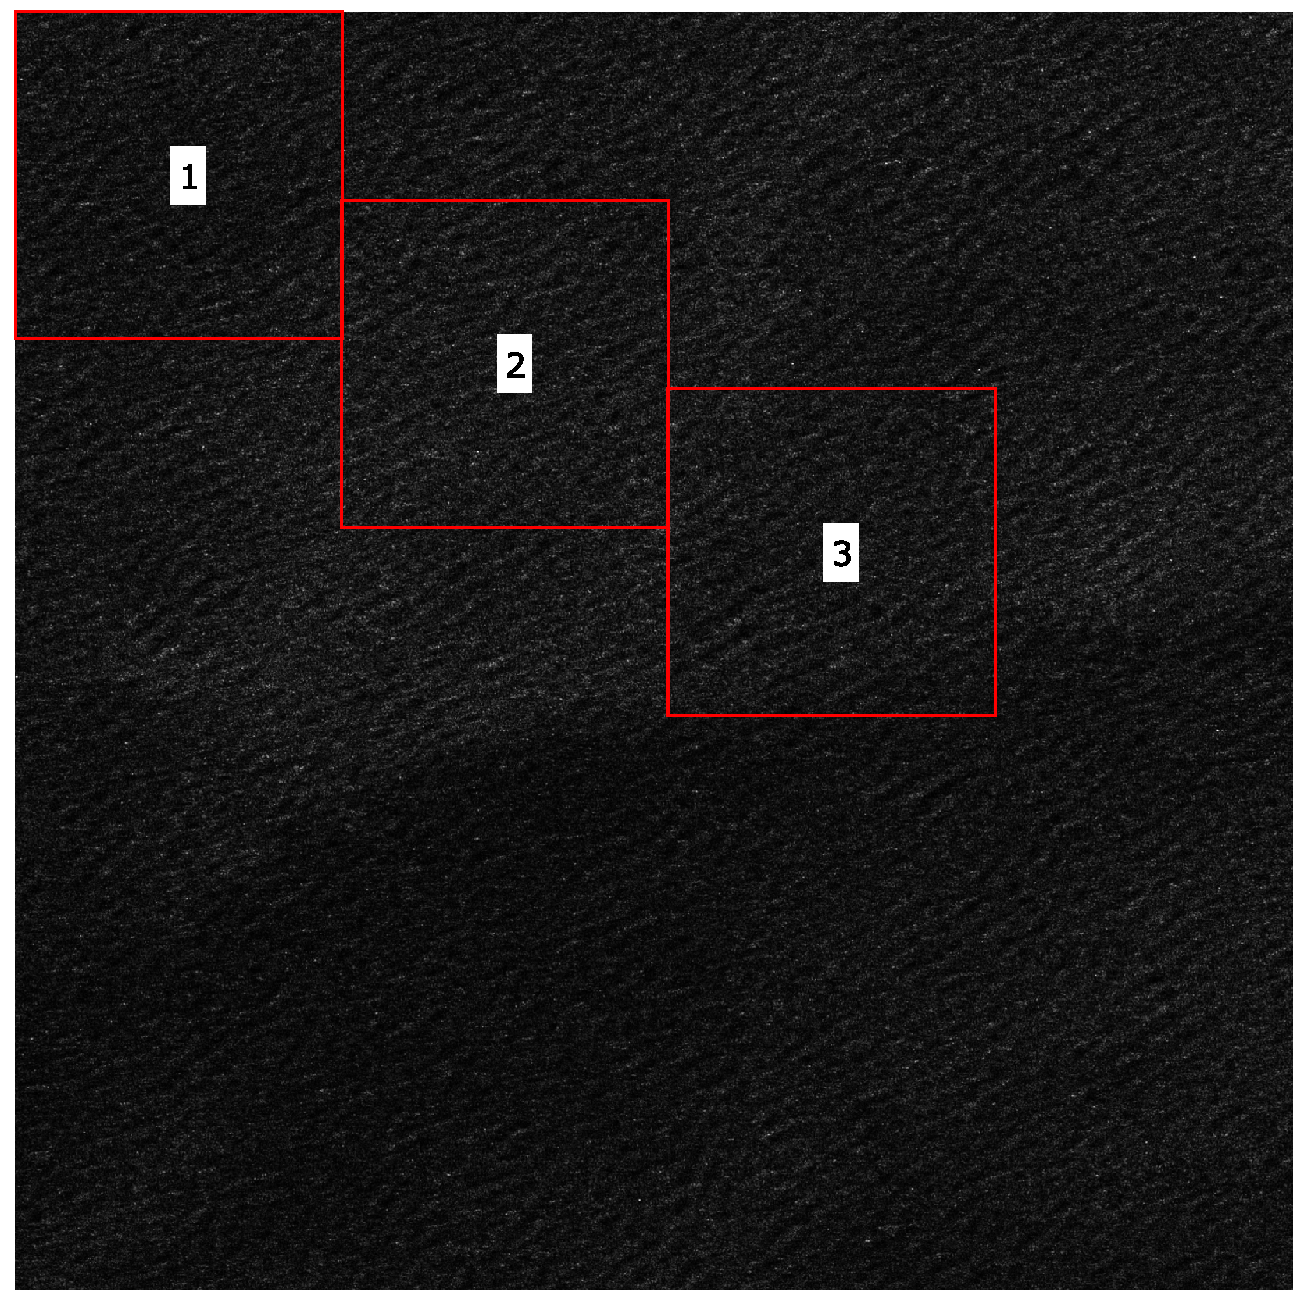
\includegraphics[width=\linewidth]{Figures/PipelineDesign/VVSceneWTransects.pdf}
        \caption{Full \acs{s1a} VV scene.}
        \label{fig:systemDesign.transectSample.full}
    \end{subfigure}   
    \begin{subfigure}{0.95\linewidth}
        \centering    
        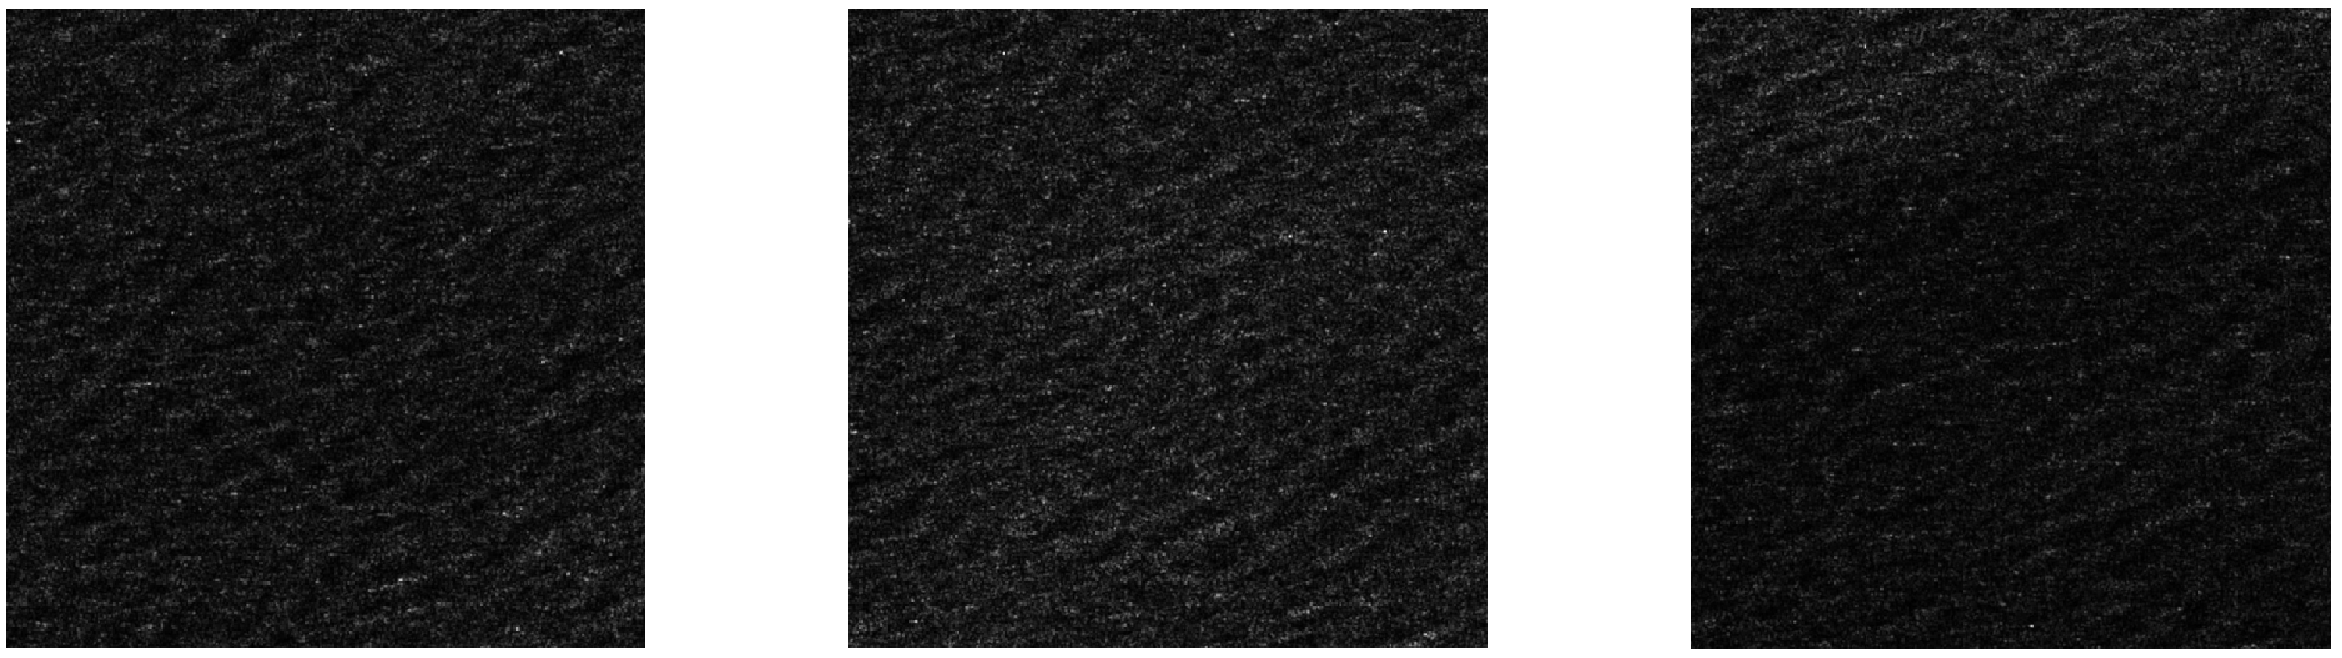
\includegraphics[width=\linewidth]{Figures/PipelineDesign/VVAllTransects.pdf}
        \caption{Transects 1 through 3 of Figure \ref{fig:systemDesign.transectSample.full} taken at 30$\degree$.}
        \label{fig:systemDesign.transectSample.all}        
    \end{subfigure}
    \caption{\acs{s1a} Intensity VV data, pre-processed according to Section \ref{sec:systemDesign.preProcessing}, from 28-Jul-2023 at 34.78\,S, 16.77\,E with transects at 30$\degree$ for $x_{1},y_{1} = 1,1$ displayed and labelled. Respective individual transects are shown.}
    \label{fig:systemDesign.transectSample}
\end{figure}
% Including geometry
% \begin{figure}[H]
%     \centering
%     \begin{subfigure}{0.48\linewidth}
%         \centering
%         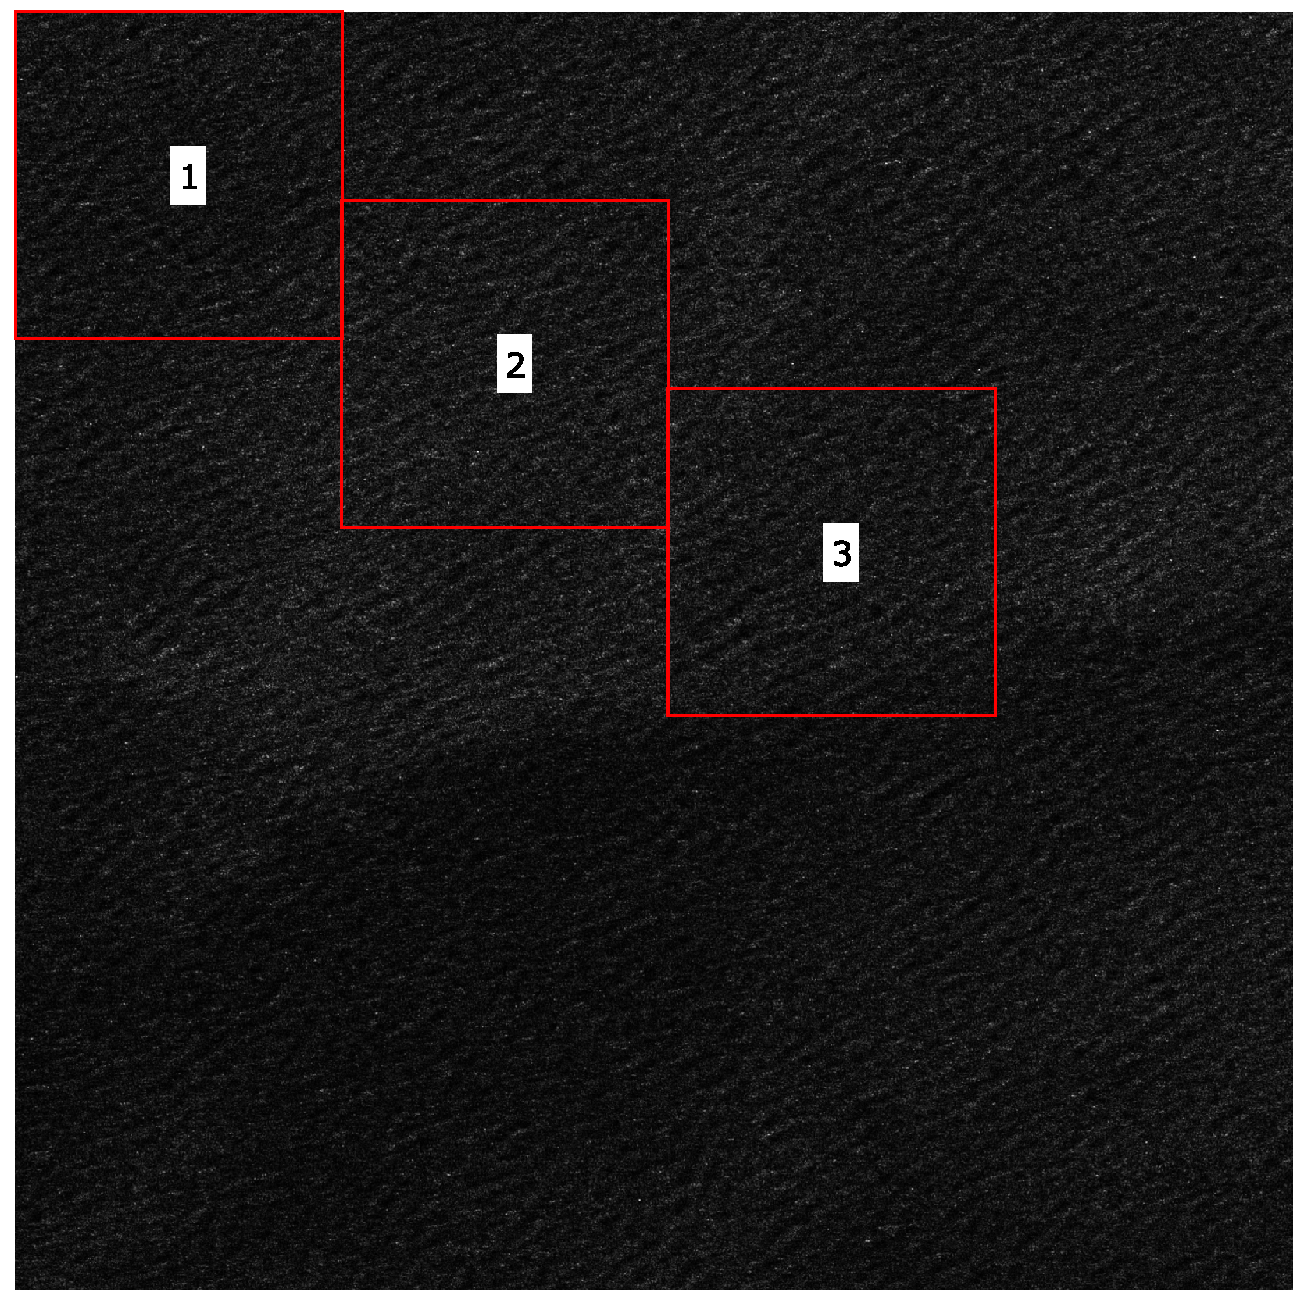
\includegraphics[width=\linewidth]{Figures/PipelineDesign/VVSceneWTransects.pdf}
%         \caption{Full \acs{s1a} VV scene.}
%         \label{fig:systemDesign.transectSample.full}
%     \end{subfigure}   
%     \begin{subfigure}{0.48\linewidth}
%         \centering
%         \includegraphics[width=\linewidth]{Figures/PipelineDesign/transects_w_SAR.pdf}
%         \caption{Full \acs{s1a} VV scene.}
%         \label{fig:systemDesign.transectSample.full}
%     \end{subfigure}    
%     \begin{subfigure}{0.95\linewidth}
%         \centering    
%         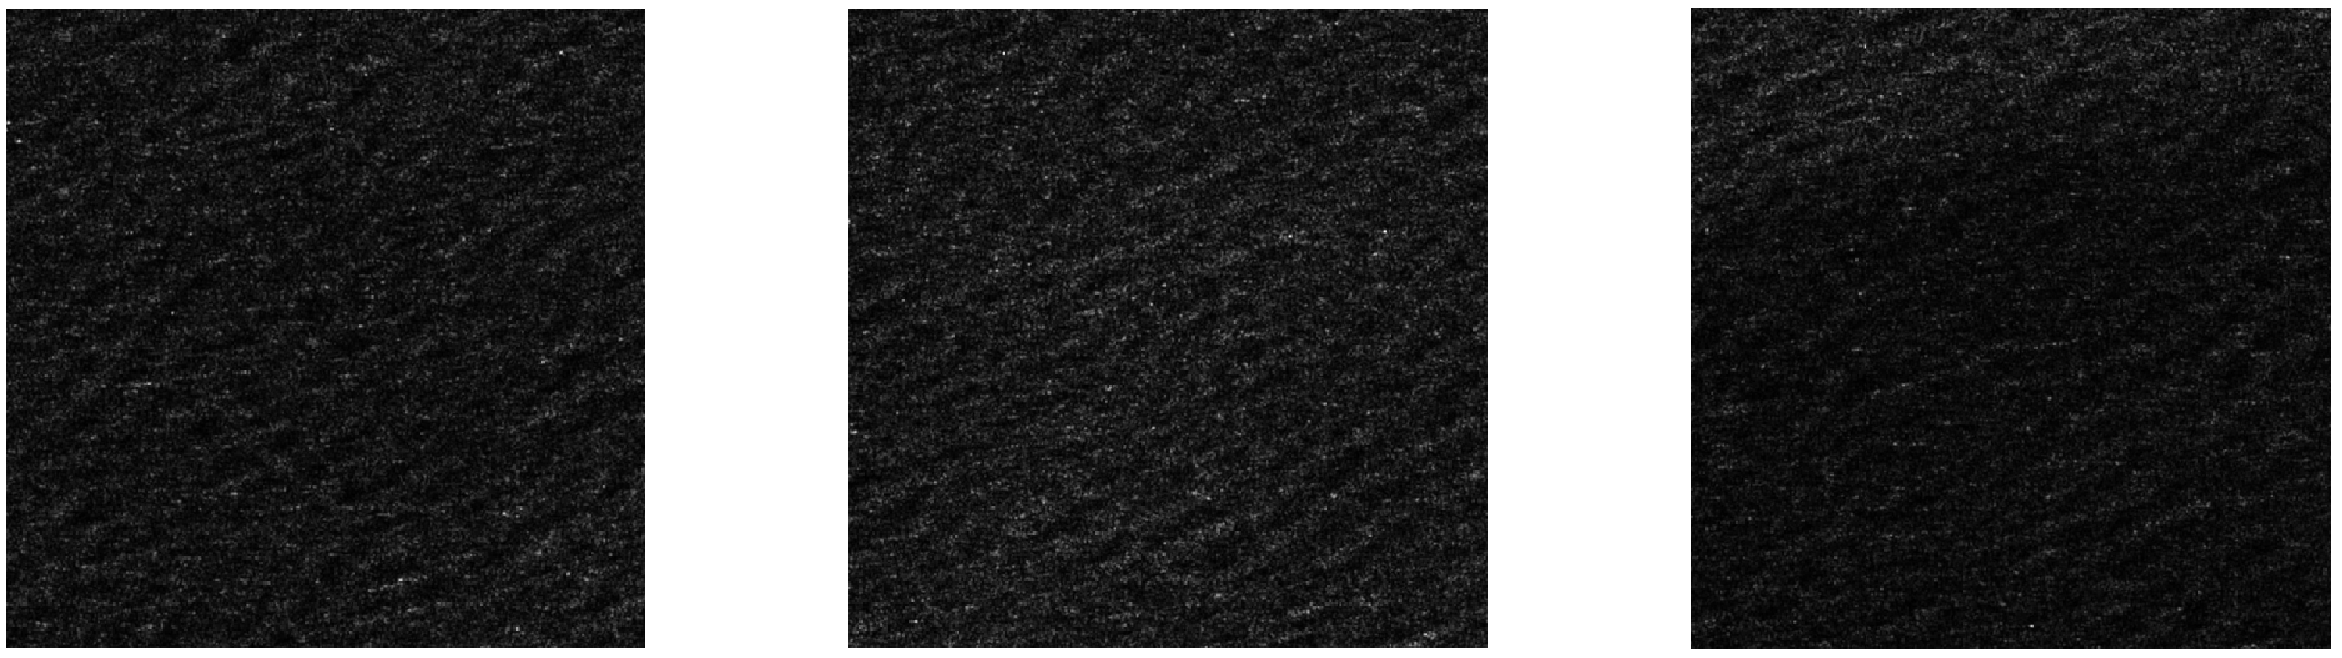
\includegraphics[width=\linewidth]{Figures/PipelineDesign/VVAllTransects.pdf}
%         \caption{Transects 1 through 3 of Figure \ref{fig:systemDesign.transectSample.full} taken at 30$\degree$.}
%         \label{fig:systemDesign.transectSample.all}        
%     \end{subfigure}
%     \caption{\acs{s1a} Intensity VV data, pre-processed according to Section \ref{sec:systemDesign.preProcessing}, from 28-Jul-2023 at 34.78\,S, 16.77\,E with transects at 30$\degree$ for $x_{1},y_{1} = 1,1$ displayed and labelled. Respective individual transects are shown.}
%     \label{fig:systemDesign.transectSample}
% \end{figure}

%====================================================
% METADATA EXTRACTION
%====================================================
\section{Metadata Extraction} \label{sec:systemDesign.metadata}

\subsection{Overview} \label{subsec:systemDesign.metadata.overview}

\begin{figure}[H]
    \centering
    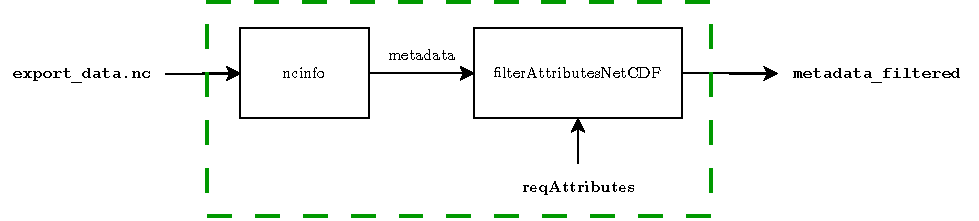
\includegraphics[width=.85\linewidth]{Figures/PipelineDesign/metadataExtraction.pdf}
    \caption{Block diagram depicting an expanded metadata extraction sub-block of Figure \ref{fig:systemDesign.scope}}
    \label{fig:systemDesign.metadata.blockDiagram}
\end{figure}

\subsection{Data Import} \label{subsec:systemDesign.metadata.import}

The first sub-block of the metadata extraction block was called \lstinline{ncinfo}. As discussed in Section \ref{subsec:systemDesign.preProcessing.exportNetCDF}, the \acs{netcdf} file format was used for importing data into \textsc{Matlab}. The \href{https://www.mathworks.com/help/Matlab/ref/ncinfo.html}{\lstinline{ncinfo}} \textsc{Matlab} function was used to import the exported data from \acs{snap} Desktop.

In order to access the exported metadata within the \acs{netcdf} file the \href{https://www.mathworks.com/help/Matlab/ref/ncinfo.html}{\lstinline{ncinfo}} \textsc{Matlab} function was used. Listing \ref{code:netCDFImport} details the required variable name to extract the metadata for the subsequent sub-block in Figure \ref{fig:systemDesign.metadata.blockDiagram}.

\begin{lstlisting}[caption={\textsc{Matlab} code used to import metadata from exported \acs{netcdf} data from \acs{snap} Desktop.},label={code:netCDFImport.metadata}]
filepath = "D:\UCT\EEE4022S\Data\CPT\export_data.nc";
metadata = ncinfo(filepath,'metadata'); % Extract all metadata
\end{lstlisting}

Using \href{https://www.mathworks.com/help/Matlab/ref/ncinfo.html}{\lstinline{ncinfo}} to extract metadata, assigns the \lstinline{metadata} variable to a $1$x$1$ structure with all desired metadata in the \texttt{Attributes} field which can be parsed to the \href{https://github.com/JNSRYA006/sar-parameter-extraction-pipeline/blob/main/functions/preprocess/annotate512Transects.m}{\lstinline{filterAttributesNetCDF}} sub-block.


\subsection{Filter Attributes} \label{subsec:systemDesign.metadata.filter}

The \href{https://github.com/JNSRYA006/sar-parameter-extraction-pipeline/blob/main/functions/preprocess/annotate512Transects.m}{\lstinline{filterAttributesNetCDF}} block takes in a structure containing metadata, as well as a list of strings of the desired attributes to keep from all metadata values. Exact attribute names can be found in Table \ref{tab:ap.metadataVals} in Appendix \ref{ap:metadata}. The function outputs a \texttt{1xlength(reqAttributes)} structure with two columns: \texttt{Name} and \texttt{Value}. Additional metadata formatting functions are discussed in Section \ref{sec:systemDesign.sarSpectrum} and \ref{sec:systemDesign.inversion} when required by respective \acp{mtf}.

%====================================================
% WAVE SPECTRUM GENERATION
%====================================================
\section{Wave Spectrum Generation} \label{sec:systemDesign.waveSpectrum}



\subsection{Overview} \label{subsec:systemDesign.waveSpectrum.Overview}

\begin{figure}[H]
    \centering
    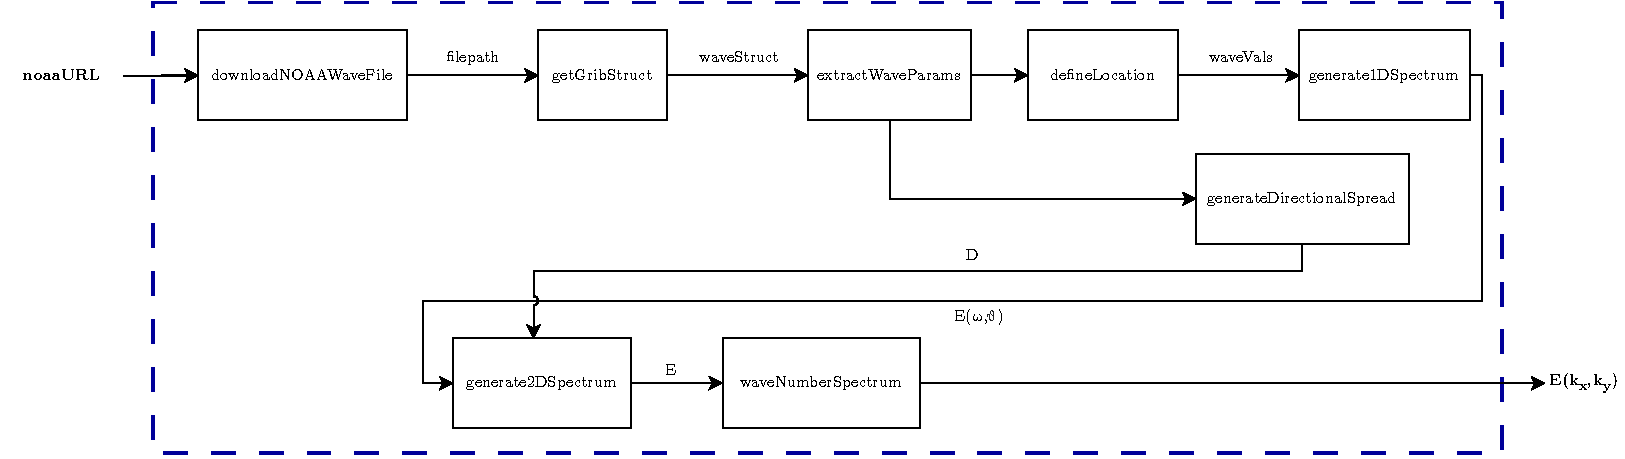
\includegraphics[width=.95\linewidth]{Figures/PipelineDesign/wave_spectrum.pdf}
    \caption{Block diagram depicting an expanded wave spectrum generation sub-block of Figure \ref{fig:systemDesign.scope}.}
    \label{fig:systemDesign.wavesSpectrum.blockDiagram}
\end{figure}

\subsection{Wave Data Download} \label{subsec:systemDesign.waveSpectrum.download}

\subsection{GRIB2 to \acs{netcdf} Conversion} \label{subsec:systemDesign.waveSpectrum.toNetCDF}

\subsection{Defining Location} \label{subsec:systemDesign.defineLocation}

The \textsc{defineLocation} sub-block in Figure \ref{fig:systemDesign.wavesSpectrum.blockDiagram} is vital to the generation of wave spectra due to the limitation of the resolution of \acs{ncep} wave data. \acs{ncep} wave data had 0.25\,degree resolution in both latitude and longitude directions, and due to the fact that the region of interest, the CSIR directional wave buoy located at $34.20400000\degree$\,S, $18.28666944\degree$\,E is not located at the points available in \acs{ncep} wave data, a grid of latitude and longitude coordinates needed to be generated surrounding the point of interest. 

This was achieved in \textsc{Matlab} using the \href{https://github.com/JNSRYA006/sar-parameter-extraction-pipeline/blob/main/functions/waveSpectra/generateSingleJONSWAP.m}{\lstinline{createLatLonGrid}} function which creates two arrays of length 3, with the three closest latitude and longitude values based on the provided latitude, longitude and resolution of wave data. This allows surrounding wave data to be extracted as detailed in Section \ref{subsec:systemDesign.waveSpectrum.parameters}. A sample output of running Listing \ref{code:latLonExtract.grid} is shown in Listing \ref{output:latLonExtract.grid}.

\begin{lstlisting}[caption={\textsc{Matlab} code used to define grid values of latitude and longitude.},label={code:latLonExtract.grid}]
latitude = 34.20400000;     % Input latitude
longitude = -18.28666944;   % Input longitude
resolution = 0.25;          % Resolution in degrees
[grid_lat, grid_lon] = createLatLonGrid(latitude, longitude, resolution);
\end{lstlisting}

\lstinputlisting[float=h,frame=tb,caption=\textsc{Matlab} output of Listing \ref{code:latLonExtract.grid}.,label={output:latLonExtract.grid}]{Figures/PipelineDesign/latLonGrid.txt}

Listing \ref{output:latLonExtract.grid} displays a 1x3 array where the centre value represents the closest value to the given \lstinline{latitude} and \lstinline{longitude} in Listing \ref{code:latLonExtract.grid}. These arrays are used in the \textsc{extractWaveParams} sub-block to define the location over which to extract wave parameters and this process is discussed in Section \ref{subsec:systemDesign.waveSpectrum.parameters}.


\subsection{Wave Parameter Extraction} \label{subsec:systemDesign.waveSpectrum.parameters}
% Intro to structures and why we want these values

When examining the latitude and longitude values obtained from \acs{ncep}, it was noted that these data points contained decimal points of order $10^{-6}$. This proved an issue when trying to index the original downloaded wave data to access a subset of these data using the code snippet depicted in Listing \ref{code:latLonExtract.initial}. This code resulted in none of the desired data being found.

\begin{lstlisting}[caption={Initial implementation of \textsc{Matlab} code to extract wave parameters at certain geographical location.},label={code:latLonExtract.initial}]
lonVal = 45.25;
lonIndex = find(lon == lonVal);
\end{lstlisting}

In order to mitigate this, an investigation into the resolution of decimal degrees was conducted in order to match the spatial resolution of wave data to the corresponding \acs{sar} resolution. It was found that 5 decimal places allowed a worst-case resolution of 1.11\,m \cite{decimalDegreesWikipedia}. In the case of \acs{s1a}, such resolution is adequate, due to the satellite's highest spatial resolution of 9x9\,m resolution for \acs{grd} data \cite{sentinel1ProductDef}. Using this information, it was decided to update the code in Listing \ref{code:latLonExtract.initial} to the code seen in Listing \ref{code:latLonExtract.round} to allow accurate indexing of spatial coordinates without loss of spatial resolution.

\begin{lstlisting}[caption={Updated implementation of \textsc{Matlab} code to extract wave parameters at certain geographical location.},label={code:latLonExtract.round}]
lonVal = 45.25;
lonIndex = find(round(lon,5) == lonVal);
\end{lstlisting}


%\subsection{Location Definition} \label{subsec:systemDesign.waveSpectrum.defineLoc}
% Put in 1D wave spectrum Generation

\subsection{One Dimensional Wave Spectrum} \label{subsec:systemDesign.waveSpectrum.1DSpectrum}

Whilst the generation of a one-dimensional wave spectrum is only represented by one sub-block in Figure \ref{fig:systemDesign.wavesSpectrum.blockDiagram}, the generation of this spectrum is vital to forming the foundation of the two-dimensional wave spectrum which is used as a first-guess wave spectrum when minimising the cost function described in Equation \ref{eq:hh.inversion.J}. As discussed in Section \ref{subsec:theory.waves.modelling}, the most widely used wave model is the \acs{jonswap} model, and implementing this spectrum required a careful approach in order to ensure accurate modelling of waves was done using the downloaded wave data detailed in Section \ref{subsec:systemDesign.waveSpectrum.download}.

In order to construct a \acs{jonswap} wave model, $E(\omega)$, the equations detailed in Section \ref{subsec:theory.waves.modelling} were implemented in \textsc{Matlab} as outlined in the pseudocode given in Algorithm \ref{alg:jonswap} where $H_{1/3}$ and $w_{peak}$ are wave parameters as detailed in Section \ref{subsec:theory.waves.modelling} and $\omega$ is the range of frequencies over which to generate the wave spectrum for. as well as defining which geographical coordinate to construct the wave spectrum for. 
%% Mention how we know what gamma value to use


\begin{figure}[H]
  \vspace{0.5cm}
  \centering
  \captionsetup{type=figure}
  \begin{minipage}{.75\linewidth}
    \begin{algorithm}[H]
      \caption{\acs{jonswap} wave spectrum generation\label{alg:jonswap}}

      \DontPrintSemicolon
      \SetAlgoLined
      \SetKwInOut{Input}{input}\SetKwInOut{Output}{output}\SetKwInOut{Parameter}{parameter}

      \Input{Wave parameters, $H_{1/3}$, $\omega_{peak}$ \\ Frequency range, $\omega$}
      \Output{\acs{jonswap} wave spectrum, $E(\omega)$}
      \Parameter{Peak enhancement factor, $\gamma$} % What is parameter

      \BlankLine
          \Begin{
          $g \leftarrow 9.81$\;
          $\alpha \leftarrow 0.2 \cdot H_{1/3}^{2} \cdot \frac{\omega_{peak}^{4}}{g^{2}}$ \;
          \If{$\gamma < 1$ or $\gamma > 7$}{
            % \If{$\gamma \neq 0$}{
            %     %\textbf{Display} warning message: "Warning: gamma value in wave_spectrum function outside validity range, using DNV formula"\;
            % }
            $k \leftarrow \frac{2\pi}{\omega_{0} \cdot \sqrt{H_{s}}}$\;
           \If{$k \leq 3.6$}{
                $\gamma \leftarrow 5$\;
           }
           \eIf{$k \leq 5$}{
                $\gamma \leftarrow \exp(5.75 - 1.15 \cdot k)$\;
           }{
                $\gamma \leftarrow 1$\;
           }
          }
        \For{$k$ in $1$ to $\text{length}(\omega)$}{
        \If{$\omega(k) < \omega_{peak}$}{
        $\sigma \leftarrow 0.07$\;
    }
    \Else{
        $\sigma \leftarrow 0.09$\;
    }
    
    $E1 \leftarrow \alpha \cdot g^2 \cdot (\omega(k)^{-5}) \cdot \exp\left(-\frac{5}{4} \cdot \left ( \frac{\omega_{peak}}{\omega(k)}\right)^4\right)$\;
    $\text{exponent} \leftarrow  \exp\left(- \frac{(\omega(k) - \omega_0)^2}{2 \cdot (\sigma \cdot \omega_0)^2}\right) $ \;
    $E2 \leftarrow \gamma^{\text{exponent}}$\;
    
    $E \leftarrow E1 \cdot E2$\;
}
        }
      \vspace{0.5cm}
    \end{algorithm}
  \end{minipage}
\end{figure}


Extending Algorithm \ref{alg:jonswap} to allow multiple spectra to be calculated at multiple latitudes and longitudes allowed the validity of the spectrum generation to be validated as plotting multiple wave spectra on the same set of axes allowed the way in which the wave spectra change as they approach the shore to be determined. This analysis is discussed in Section xxx and example plots obtained using the \href{https://github.com/JNSRYA006/sar-parameter-extraction-pipeline/blob/main/functions/waveSpectra/generateSingleJONSWAP.m}{\lstinline{generateSingleJONSWAP}} and \href{https://github.com/JNSRYA006/sar-parameter-extraction-pipeline/blob/main/functions/waveSpectra/generateMultipleJONSWAP.m}{\lstinline{generateMultipleJONSWAP}} functions are shown in Figure \ref{fig:systemDesign.1DSampleWaveSpectrum}. 

% \begin{figure}[H]
% \centering
% \begin{subfigure}{0.48\linewidth} % Use \begin{subfigure} instead of \begin{subfigure}
%     \resizebox{\linewidth}{!}{% This file was created by matlab2tikz.
%
%The latest updates can be retrieved from
%  http://www.mathworks.com/matlabcentral/fileexchange/22022-matlab2tikz-matlab2tikz
%where you can also make suggestions and rate matlab2tikz.
%
\definecolor{mycolor1}{rgb}{0.00000,0.44700,0.74100}%
%
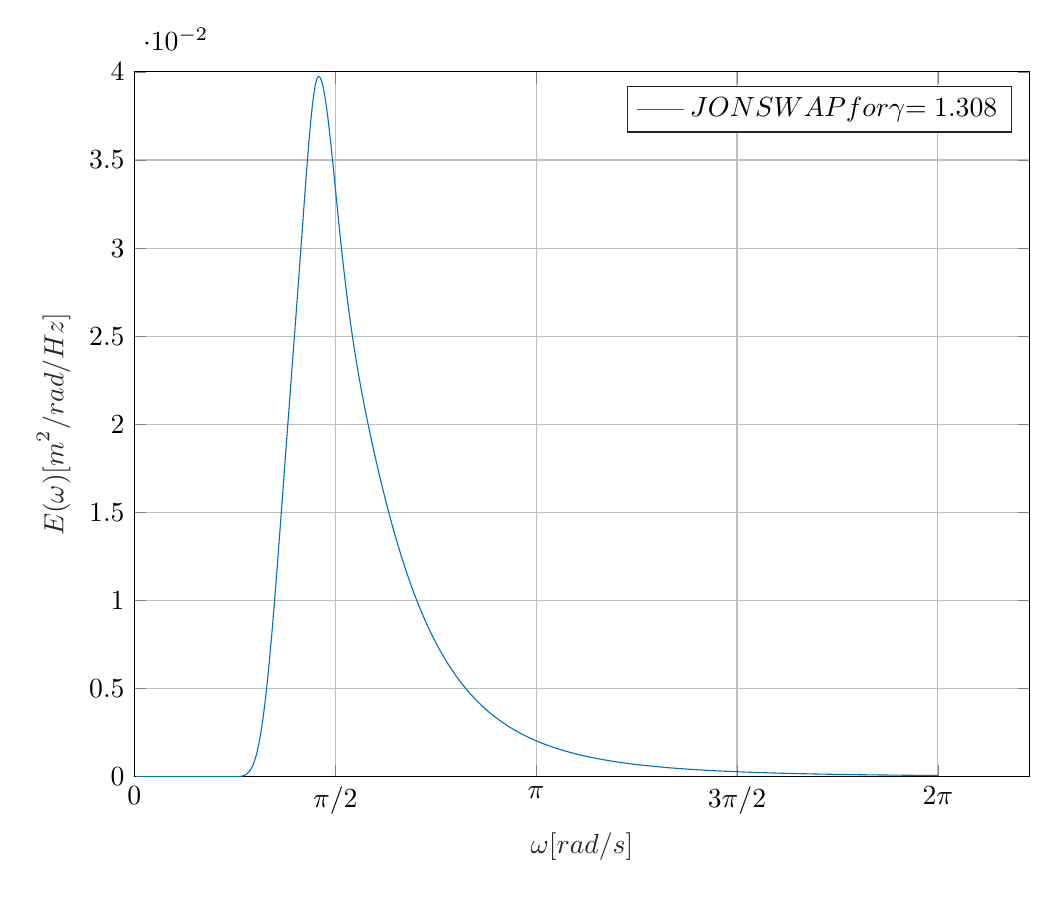
\begin{tikzpicture}

\begin{axis}[%
width=4.476in,
height=3.524in,
at={(0.803in,0.523in)},
scale only axis,
unbounded coords=jump,
xmin=0,
xmax=7,
xtick={0,1.5707963267949,3.14159265358979,4.71238898038469,6.28318530717959},
xticklabels={{0},{$\pi\text{/2}$},{$\pi$},{$\text{3}\pi\text{/2}$},{$\text{2}\pi$}},
xlabel style={font=\color{white!15!black}},
xlabel={$\omega\text{ [rad/s]}$},
ymin=0,
ymax=0.04,
ylabel style={font=\color{white!15!black}},
ylabel={$\text{E(}\omega\text{) [m}^\text{2}\text{/rad/Hz]}$},
axis background/.style={fill=white},
title style={font=\bfseries},
%title={$\text{One-dimensional wave spectrum, E(}\omega\text{) at -34S, 17.25E}$},
xmajorgrids,
ymajorgrids,
legend style={legend cell align=left, align=left, draw=white!15!black}
]
\addplot [color=mycolor1]
  table[row sep=crcr]{%
0	nan\\
0.0122958616578857	0\\
0.0245917233157714	0\\
0.0368875849736571	0\\
0.0491834466315427	0\\
0.0614793082894284	0\\
0.0737751699473141	0\\
0.0860710316051998	0\\
0.0983668932630855	0\\
0.110662754920971	0\\
0.122958616578857	0\\
0.135254478236743	0\\
0.147550339894628	0\\
0.159846201552514	0\\
0.1721420632104	0\\
0.184437924868285	0\\
0.196733786526171	0\\
0.209029648184057	0\\
0.221325509841942	0\\
0.233621371499828	0\\
0.245917233157714	0\\
0.258213094815599	0\\
0.270508956473485	0\\
0.282804818131371	0\\
0.295100679789256	5.41302879763333e-307\\
0.307396541447142	1.4351658983951e-260\\
0.319692403105028	1.39801651640755e-222\\
0.331988264762914	2.95955173493782e-191\\
0.344284126420799	3.06617261869068e-165\\
0.356579988078685	1.71585454184354e-143\\
0.368875849736571	3.36115162791715e-125\\
0.381171711394456	9.99471845091621e-110\\
0.393467573052342	1.44074967318733e-96\\
0.405763434710228	2.54134308132756e-85\\
0.418059296368113	1.15384979645612e-75\\
0.430355158025999	2.46010694641464e-67\\
0.442651019683885	4.01707121559874e-60\\
0.45494688134177	7.49671131280128e-54\\
0.467242742999656	2.22288404307939e-48\\
0.479538604657542	1.3753760835859e-43\\
0.491834466315427	2.22745866619101e-39\\
0.504130327973313	1.14105811314078e-35\\
0.516426189631199	2.16730148431401e-32\\
0.528722051289085	1.74501685936915e-29\\
0.54101791294697	6.67054290550385e-27\\
0.553313774604856	1.33294088654399e-24\\
0.565609636262742	1.51145852287043e-22\\
0.577905497920627	1.0433270916913e-20\\
0.590201359578513	4.65664898554377e-19\\
0.602497221236399	1.41551545559892e-17\\
0.614793082894284	3.06504085545376e-16\\
0.62708894455217	4.91508596715723e-15\\
0.639384806210056	6.03782647089776e-14\\
0.651680667867941	5.85166582657271e-13\\
0.663976529525827	4.59100381164424e-12\\
0.676272391183713	2.98235025750544e-11\\
0.688568252841599	1.63618607596188e-10\\
0.700864114499484	7.71435740175365e-10\\
0.71315997615737	3.17422780050511e-09\\
0.725455837815256	1.15545266932238e-08\\
0.737751699473141	3.76593918002615e-08\\
0.750047561131027	1.11082567474578e-07\\
0.762343422788913	2.99365257438456e-07\\
0.774639284446798	7.43398794457705e-07\\
0.786935146104684	1.71393732492197e-06\\
0.79923100776257	3.6936978163335e-06\\
0.811526869420455	7.48610717182671e-06\\
0.823822731078341	1.43464290828625e-05\\
0.836118592736227	2.61246562604755e-05\\
0.848414454394112	4.54036148623333e-05\\
0.860710316051998	7.56117606150625e-05\\
0.873006177709884	0.000121089372916668\\
0.88530203936777	0.000187089786772187\\
0.897597901025655	0.000279703606526386\\
0.909893762683541	0.000405702450085907\\
0.922189624341426	0.000572308176547121\\
0.934485485999312	0.000786902195884214\\
0.946781347657198	0.00105669606424971\\
0.959077209315084	0.00138838834019309\\
0.971373070972969	0.00178783338397504\\
0.983668932630855	0.00225974569705202\\
0.995964794288741	0.00280745915996462\\
1.00826065594663	0.00343275496464683\\
1.02055651760451	0.00413576600873186\\
1.0328523792624	0.00491495977802167\\
1.04514824092028	0.00576719685342651\\
1.05744410257817	0.00668785847600663\\
1.06973996423605	0.00767103419145496\\
1.08203582589394	0.00870975936699404\\
1.09433168755183	0.0097962920536587\\
1.10662754920971	0.0109224188636112\\
1.1189234108676	0.0120797798007726\\
1.13121927252548	0.0132602018978306\\
1.14351513418337	0.0144560307440969\\
1.15581099584125	0.0156604473784329\\
1.16810685749914	0.0168677556407375\\
1.18040271915703	0.0180736222488931\\
1.19269858081491	0.0192752491472963\\
1.2049944424728	0.0204714557558278\\
1.21729030413068	0.0216626483564445\\
1.22958616578857	0.0228506556097147\\
1.24188202744645	0.0240384135360737\\
1.25417788910434	0.0252294904939306\\
1.26647375076223	0.0264274529344006\\
1.27876961242011	0.0276350862726403\\
1.291065474078	0.0288535024756524\\
1.30336133573588	0.0300811872588852\\
1.31565719739377	0.0313130648442189\\
1.32795305905165	0.0325396852882558\\
1.34024892070954	0.0337466641153829\\
1.35254478236743	0.0349145188355605\\
1.36484064402531	0.0360190415875961\\
1.3771365056832	0.0370323108877261\\
1.38943236734108	0.0379243714742074\\
1.40172822899897	0.0386655021114703\\
1.41402409065685	0.0392288631897149\\
1.42631995231474	0.0395931988386078\\
1.43861581397263	0.0397451987880671\\
1.45091167563051	0.0397009837064543\\
1.4632075372884	0.0395060933162202\\
1.47550339894628	0.0391703952648501\\
1.48779926060417	0.0387059506556059\\
1.50009512226205	0.0381276193041899\\
1.51239098391994	0.0374522472133023\\
1.52468684557783	0.0366977905296433\\
1.53698270723571	0.0358824534634019\\
1.5492785688936	0.0350239067515314\\
1.56157443055148	0.0341386357865274\\
1.57387029220937	0.033241447182027\\
1.58616615386725	0.0323451427488864\\
1.59846201552514	0.0314603532066003\\
1.61075787718303	0.0305955119179262\\
1.62305373884091	0.0297569418708591\\
1.6353496004988	0.0289490265523619\\
1.64764546215668	0.0281744362672717\\
1.65994132381457	0.0274343846835443\\
1.67223718547245	0.0267288948374096\\
1.68453304713034	0.0260570586376697\\
1.69682890878822	0.0254172784703886\\
1.70912477044611	0.0248074834845985\\
1.721420632104	0.024225316400738\\
1.73371649376188	0.023668289227364\\
1.74601235541977	0.0231339081746281\\
1.75830821707765	0.0226197694201764\\
1.77060407873554	0.0221236283185714\\
1.78289994039342	0.0216434452374737\\
1.79519580205131	0.0211774115218765\\
1.8074916637092	0.0207239591846428\\
1.81978752536708	0.0202817578397189\\
1.83208338702497	0.0198497021705522\\
1.84437924868285	0.0194268928954684\\
1.85667511034074	0.0190126137886203\\
1.86897097199862	0.0186063068732881\\
1.88126683365651	0.0182075474549375\\
1.8935626953144	0.0178160202313337\\
1.90585855697228	0.0174314973270267\\
1.91815441863017	0.0170538187637728\\
1.93045028028805	0.0166828756042898\\
1.94274614194594	0.0163185957954444\\
1.95504200360382	0.0159609325850235\\
1.96733786526171	0.0156098552867384\\
1.9796337269196	0.015265342112225\\
1.99192958857748	0.0149273747670556\\
2.00422545023537	0.0145959345109985\\
2.01652131189325	0.0142709994027779\\
2.02881717355114	0.0139525424796016\\
2.04111303520902	0.0136405306563983\\
2.05340889686691	0.0133349241651845\\
2.0657047585248	0.0130356763886258\\
2.07800062018268	0.0127427339721329\\
2.09029648184057	0.0124560371249502\\
2.10259234349845	0.0121755200424896\\
2.11488820515634	0.0119011113998192\\
2.12718406681422	0.0116327348801607\\
2.13947992847211	0.011370309712995\\
2.15177579012999	0.0111137512044894\\
2.16407165178788	0.0108629712489418\\
2.17636751344577	0.0106178788142673\\
2.18866337510365	0.0103783803976124\\
2.20095923676154	0.0101443804493013\\
2.21325509841942	0.00991578176473845\\
2.22555096007731	0.00969248584482827\\
2.2378468217352	0.00947439322604724\\
2.25014268339308	0.00926140378164897\\
2.26243854505097	0.0090534169956585\\
2.27473440670885	0.00885033221138453\\
2.28703026836674	0.00865204885617913\\
2.29932613002462	0.00845846664413426\\
2.31162199168251	0.00826948575833719\\
2.3239178533404	0.00808500701422663\\
2.33621371499828	0.00790493200550391\\
2.34850957665617	0.00772916323396475\\
2.36080543831405	0.00755760422452847\\
2.37310129997194	0.00739015962665654\\
2.38539716162982	0.00722673530327022\\
2.39769302328771	0.00706723840819925\\
2.40998888494559	0.00691157745312068\\
2.42228474660348	0.0067596623648772\\
2.43458060826137	0.00661140453400037\\
2.44687646991925	0.00646671685520286\\
2.45917233157714	0.00632551376054758\\
2.47146819323502	0.00618771124594853\\
2.48376405489291	0.00605322689160874\\
2.49605991655079	0.00592197987695489\\
2.50835577820868	0.00579389099058502\\
2.52065163986657	0.00566888263570622\\
2.53294750152445	0.00554687883150177\\
2.54524336318234	0.00542780521083287\\
2.55753922484022	0.00531158901464808\\
2.56983508649811	0.00519815908344373\\
2.58213094815599	0.00508744584609102\\
2.59442680981388	0.00497938130631981\\
2.60672267147177	0.00487389902712567\\
2.61901853312965	0.00477093411334424\\
2.63131439478754	0.00467042319261705\\
2.64361025644542	0.00457230439495386\\
2.65590611810331	0.00447651733107909\\
2.66820197976119	0.00438300306973388\\
2.68049784141908	0.00429170411409041\\
2.69279370307697	0.00420256437742111\\
2.70508956473485	0.00411552915815301\\
2.71738542639274	0.00403054511442532\\
2.72968128805062	0.00394756023825787\\
2.74197714970851	0.00386652382942774\\
2.75427301136639	0.00378738646914243\\
2.76656887302428	0.00371009999358922\\
2.77886473468217	0.00363461746743274\\
2.79116059634005	0.00356089315732546\\
2.80345645799794	0.00348888250548924\\
2.81575231965582	0.00341854210342006\\
2.82804818131371	0.00334982966576232\\
2.84034404297159	0.00328270400439414\\
2.85263990462948	0.00321712500276036\\
2.86493576628737	0.00315305359048552\\
2.87723162794525	0.00309045171829528\\
2.88952748960314	0.00302928233327117\\
2.90182335126102	0.0029695093544601\\
2.91411921291891	0.00291109764885714\\
2.92641507457679	0.00285401300777748\\
2.93871093623468	0.00279822212363068\\
2.95100679789256	0.00274369256710825\\
2.96330265955045	0.00269039276479353\\
2.97559852120834	0.00263829197720089\\
2.98789438286622	0.00258736027724954\\
3.00019024452411	0.00253756852917576\\
3.01248610618199	0.00248888836788607\\
3.02478196783988	0.00244129217875227\\
3.03707782949776	0.00239475307784859\\
3.04937369115565	0.00234924489262979\\
3.06166955281354	0.0023047421430484\\
3.07396541447142	0.0022612200231083\\
3.08626127612931	0.00221865438285134\\
3.09855713778719	0.00217702171077273\\
3.11085299944508	0.00213629911666074\\
3.12314886110296	0.00209646431485547\\
3.13544472276085	0.00205749560792113\\
3.14774058441874	0.00201937187072593\\
3.16003644607662	0.00198207253492326\\
3.17233230773451	0.00194557757382764\\
3.18462816939239	0.00190986748767868\\
3.19692403105028	0.00187492328928602\\
3.20921989270816	0.00184072649004824\\
3.22151575436605	0.00180725908633834\\
3.23381161602394	0.00177450354624858\\
3.24610747768182	0.00174244279668723\\
3.25840333933971	0.00171106021081969\\
3.27069920099759	0.0016803395958467\\
3.28299506265548	0.00165026518111192\\
3.29529092431336	0.00162082160653164\\
3.30758678597125	0.00159199391133908\\
3.31988264762914	0.00156376752313587\\
3.33217850928702	0.00153612824724346\\
3.34447437094491	0.00150906225634721\\
3.35677023260279	0.00148255608042589\\
3.36906609426068	0.00145659659695957\\
3.38136195591856	0.00143117102140895\\
3.39365781757645	0.00140626689795909\\
3.40595367923434	0.00138187209052092\\
3.41824954089222	0.00135797477398379\\
3.43054540255011	0.00133456342571239\\
3.44284126420799	0.00131162681728186\\
3.45513712586588	0.00128915400644448\\
3.46743298752376	0.00126713432932197\\
3.47972884918165	0.00124555739281723\\
3.49202471083954	0.00122441306723957\\
3.50432057249742	0.00120369147913769\\
3.51661643415531	0.00118338300433464\\
3.52891229581319	0.00116347826115928\\
3.54120815747108	0.00114396810386871\\
3.55350401912896	0.00112484361625655\\
3.56579988078685	0.0011060961054416\\
3.57809574244473	0.00108771709583218\\
3.59039160410262	0.00106969832326091\\
3.60268746576051	0.00105203172928534\\
3.61498332741839	0.00103470945564963\\
3.62727918907628	0.0010177238389028\\
3.63957505073416	0.00100106740516895\\
3.65187091239205	0.000984732865065375\\
3.66416677404994	0.000968713108764074\\
3.67646263570782	0.00095300120119279\\
3.68875849736571	0.00093759037737141\\
3.70105435902359	0.000922474037879949\\
3.71335022068148	0.000907645744454282\\
3.72564608233936	0.000893099215705966\\
3.73794194399725	0.000878828322962575\\
3.75023780565513	0.000864827086225059\\
3.76253366731302	0.000851089670238769\\
3.77482952897091	0.000837610380674829\\
3.78712539062879	0.000824383660418703\\
3.79942125228668	0.000811404085962812\\
3.81171711394456	0.00079866636390022\\
3.82401297560245	0.000786165327516438\\
3.83630883726033	0.000773895933476511\\
3.84860469891822	0.000761853258604621\\
3.86090056057611	0.000750032496753526\\
3.87319642223399	0.000738428955761214\\
3.88549228389188	0.000727038054492271\\
3.89778814554976	0.000715855319961465\\
3.91008400720765	0.000704876384537197\\
3.92237986886553	0.000694096983222478\\
3.93467573052342	0.000683512951011199\\
3.94697159218131	0.000673120220317491\\
3.95926745383919	0.000662914818476088\\
3.97156331549708	0.000652892865311599\\
3.98385917715496	0.000643050570774724\\
3.99615503881285	0.000633384232643455\\
4.00845090047073	0.000623890234287399\\
4.02074676212862	0.000614565042493382\\
4.03304262378651	0.000605405205350579\\
4.04533848544439	0.000596407350193436\\
4.05763434710228	0.000587568181600735\\
4.06993020876016	0.000578884479449159\\
4.08222607041805	0.00057035309701982\\
4.09452193207593	0.000561970959156189\\
4.10681779373382	0.000553735060471986\\
4.1191136553917	0.000545642463607562\\
4.13140951704959	0.000537690297533413\\
4.14370537870748	0.00052987575589945\\
4.15600124036536	0.000522196095428724\\
4.16829710202325	0.000514648634354346\\
4.18059296368113	0.00050723075089834\\
4.19288882533902	0.00049993988179127\\
4.2051846869969	0.000492773520831441\\
4.21748054865479	0.00048572921748257\\
4.22977641031268	0.000478804575508837\\
4.24207227197056	0.000471997251646233\\
4.25436813362845	0.000465304954309197\\
4.26666399528633	0.000458725442331523\\
4.27895985694422	0.000452256523740597\\
4.29125571860211	0.000445896054563984\\
4.30355158025999	0.000439641937667487\\
4.31584744191788	0.000433492121623766\\
4.32814330357576	0.000427444599610678\\
4.34043916523365	0.000421497408338488\\
4.35273502689153	0.000415648627005148\\
4.36503088854942	0.000409896376278856\\
4.37732675020731	0.000404238817307136\\
4.38962261186519	0.000398674150751693\\
4.40191847352308	0.000393200615848326\\
4.41421433518096	0.000387816489491206\\
4.42651019683885	0.000382520085340833\\
4.43880605849673	0.000377309752955029\\
4.45110192015462	0.000372183876942308\\
4.46339778181251	0.000367140876137024\\
4.47569364347039	0.000362179202795692\\
4.48798950512828	0.000357297341813879\\
4.50028536678616	0.000352493809963128\\
4.51258122844405	0.000347767155147345\\
4.52487709010193	0.000343115955678117\\
4.53717295175982	0.000338538819568452\\
4.5494688134177	0.000334034383844427\\
4.56176467507559	0.000329601313874257\\
4.57406053673348	0.000325238302714321\\
4.58635639839136	0.000320944070471665\\
4.59865226004925	0.000316717363682552\\
4.61094812170713	0.000312556954706612\\
4.62324398336502	0.00030846164113618\\
4.6355398450229	0.000304430245220401\\
4.64783570668079	0.000300461613303707\\
4.66013156833868	0.000296554615278295\\
4.67242742999656	0.000292708144050196\\
4.68472329165445	0.000288921115018604\\
4.69701915331233	0.000285192465568094\\
4.70931501497022	0.000281521154573383\\
4.7216108766281	0.000277906161916305\\
4.73390673828599	0.000274346488014674\\
4.74620259994388	0.000270841153362717\\
4.75849846160176	0.000267389198082769\\
4.77079432325965	0.000263989681487935\\
4.78309018491753	0.000260641681655428\\
4.79538604657542	0.000257344295010299\\
4.8076819082333	0.000254096635919287\\
4.81997776989119	0.000250897836294526\\
4.83227363154908	0.000247747045206839\\
4.84456949320696	0.000244643428508389\\
4.85686535486485	0.000241586168464416\\
4.86916121652273	0.000238574463393844\\
4.88145707818062	0.000235607527318515\\
4.8937529398385	0.000232684589620834\\
4.90604880149639	0.000229804894709597\\
4.91834466315427	0.000226967701693801\\
4.93064052481216	0.000224172284064218\\
4.94293638647005	0.000221417929382543\\
4.95523224812793	0.000218703938977918\\
4.96752810978582	0.000216029627650631\\
4.9798239714437	0.000213394323382829\\
4.99211983310159	0.000210797367056043\\
5.00441569475948	0.000208238112175362\\
5.01671155641736	0.000205715924600084\\
5.02900741807525	0.000203230182280682\\
5.04130327973313	0.000200780275001916\\
5.05359914139102	0.000198365604131947\\
5.0658950030489	0.000195985582377289\\
5.07819086470679	0.00019363963354346\\
5.09048672636467	0.000191327192301187\\
5.10278258802256	0.000189047703958018\\
5.11507844968045	0.000186800624235214\\
5.12737431133833	0.00018458541904979\\
5.13967017299622	0.000182401564301559\\
5.1519660346541	0.000180248545665076\\
5.16426189631199	0.000178125858386348\\
5.17655775796987	0.000176033007084189\\
5.18885361962776	0.000173969505556115\\
5.20114948128565	0.000171934876588657\\
5.21344534294353	0.000169928651771981\\
5.22574120460142	0.000167950371318724\\
5.2380370662593	0.000165999583886923\\
5.25033292791719	0.000164075846406948\\
5.26262878957507	0.000162178723912337\\
5.27492465123296	0.000160307789374435\\
5.28722051289085	0.000158462623540752\\
5.29951637454873	0.000156642814776941\\
5.31181223620662	0.000154847958912307\\
5.3241080978645	0.000153077659088771\\
5.33640395952239	0.000151331525613192\\
5.34869982118027	0.000149609175812981\\
5.36099568283816	0.000147910233894908\\
5.37329154449605	0.000146234330807043\\
5.38558740615393	0.000144581104103749\\
5.39788326781182	0.000142950197813643\\
5.4101791294697	0.000141341262310475\\
5.42247499112759	0.000139753954186838\\
5.43477085278547	0.000138187936130644\\
5.44706671444336	0.000136642876804307\\
5.45936257610125	0.000135118450726565\\
5.47165843775913	0.000133614338156872\\
5.48395429941702	0.00013213022498231\\
5.4962501610749	0.00013066580260695\\
5.50854602273279	0.000129220767843618\\
5.52084188439067	0.000127794822807993\\
5.53313774604856	0.000126387674814993\\
5.54543360770645	0.000124999036277395\\
5.55772946936433	0.000123628624606628\\
5.57002533102222	0.000122276162115703\\
5.5823211926801	0.00012094137592421\\
5.59461705433799	0.000119623997865353\\
5.60691291599587	0.000118323764394966\\
5.61920877765376	0.00011704041650246\\
5.63150463931164	0.000115773699623671\\
5.64380050096953	0.000114523363555545\\
5.65609636262742	0.000113289162372638\\
5.6683922242853	0.00011207085434537\\
5.68068808594319	0.000110868201860007\\
5.69298394760107	0.000109680971340328\\
5.70527980925896	0.00010850893317093\\
5.71757567091684	0.000107351861622146\\
5.72987153257473	0.000106209534776526\\
5.74216739423262	0.000105081734456864\\
5.7544632558905	0.000103968246155711\\
5.76675911754839	0.000102868858966361\\
5.77905497920627	0.000101783365515268\\
5.79135084086416	0.000100711561895862\\
5.80364670252204	9.96532476037344e-05\\
5.81594256417993	9.86082254731543e-05\\
5.82823842583782	9.75763016149018e-05\\
5.8405342874957	9.65572853553714e-05\\
5.85283014915359	9.55509891769276e-05\\
5.86512601081147	9.455722865948e-05\\
5.87742187246936	9.35758224232536e-05\\
5.88971773412724	9.26065920727251e-05\\
5.90201359578513	9.16493621417014e-05\\
5.91430945744302	9.07039600395125e-05\\
5.9266053191009	8.97702159982964e-05\\
5.93890118075879	8.88479630213512e-05\\
5.95119704241667	8.79370368325295e-05\\
5.96349290407456	8.70372758266536e-05\\
5.97578876573244	8.61485210209284e-05\\
5.98808462739033	8.5270616007331e-05\\
6.00038048904822	8.4403406905953e-05\\
6.0126763507061	8.35467423192785e-05\\
6.02497221236399	8.27004732873734e-05\\
6.03726807402187	8.18644532439695e-05\\
6.04956393567976	8.10385379734214e-05\\
6.06185979733764	8.02225855685183e-05\\
6.07415565899553	7.94164563891332e-05\\
6.08645152065342	7.86200130216882e-05\\
6.0987473823113	7.78331202394225e-05\\
6.11104324396919	7.70556449634419e-05\\
6.12333910562707	7.62874562245356e-05\\
6.13563496728496	7.55284251257423e-05\\
6.14793082894284	7.4778424805651e-05\\
6.16022669060073	7.40373304024179e-05\\
6.17252255225862	7.33050190184887e-05\\
6.1848184139165	7.25813696860062e-05\\
6.19711427557439	7.18662633328921e-05\\
6.20941013723227	7.11595827495877e-05\\
6.22170599889016	7.04612125564384e-05\\
6.23400186054804	6.97710391717103e-05\\
6.24629772220593	6.90889507802242e-05\\
6.25859358386381	6.84148373025936e-05\\
6.2708894455217	6.77485903650559e-05\\
6.28318530717959	6.70901032698821e-05\\
};
\addlegendentry{$\text{JONSWAP for }\gamma\text{ = 1.308}$}

\end{axis}
\end{tikzpicture}%}
%     \caption{\acs{jonswap} spectrum at -34S, 17.25E}
%     \label{fig:systemDesign.1DSampleWaveSpectrumSingle}   
% \end{subfigure}
% \begin{subfigure}{0.48\linewidth} % Use \begin{subfigure} instead of \begin{subfigure}
%     \resizebox{\linewidth}{!}{% This file was created by matlab2tikz.
%
%The latest updates can be retrieved from
%  http://www.mathworks.com/matlabcentral/fileexchange/22022-matlab2tikz-matlab2tikz
%where you can also make suggestions and rate matlab2tikz.
%
\definecolor{mycolor1}{rgb}{0.00000,0.44700,0.74100}%
\definecolor{mycolor2}{rgb}{0.85000,0.32500,0.09800}%
\definecolor{mycolor3}{rgb}{0.92900,0.69400,0.12500}%
%
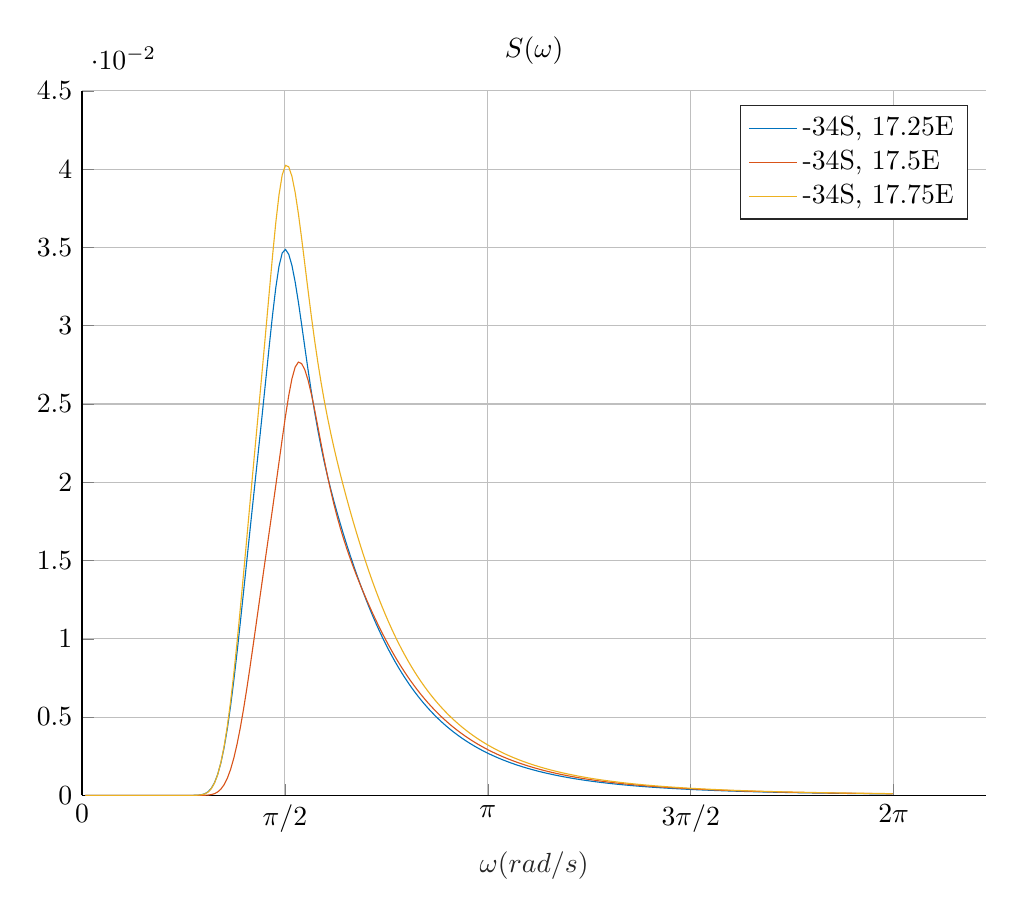
\begin{tikzpicture}

\begin{axis}[%
width=4.521in,
height=3.522in,
at={(0.758in,0.525in)},
scale only axis,
unbounded coords=jump,
xmin=0,
xmax=7,
xtick={0,1.5707963267949,3.14159265358979,4.71238898038469,6.28318530717959},
xticklabels={{0},{$\pi\text{/2}$},{$\pi$},{$\text{3}\pi\text{/2}$},{$\text{2}\pi$}},
xlabel style={font=\color{white!15!black}},
xlabel={$\omega\text{ (rad/s)}$},
ymin=0,
ymax=0.045,
axis background/.style={fill=white},
title style={font=\bfseries},
title={$\text{S(}\omega\text{)}$},
axis x line*=bottom,
axis y line*=left,
xmajorgrids,
ymajorgrids,
legend style={legend cell align=left, align=left, draw=white!15!black}
]
\addplot [color=mycolor1]
  table[row sep=crcr]{%
0	nan\\
0.025	0\\
0.05	0\\
0.075	0\\
0.1	0\\
0.125	0\\
0.15	0\\
0.175	0\\
0.2	0\\
0.225	0\\
0.25	0\\
0.275	0\\
0.3	0\\
0.325	1.42005336164696e-294\\
0.35	9.69071650364021e-219\\
0.375	8.9429723835081e-166\\
0.4	6.86905098134045e-128\\
0.425	3.20255852046391e-100\\
0.45	1.21756251134366e-79\\
0.475	4.39413653830271e-64\\
0.5	3.75253612752824e-52\\
0.525	6.98108061469795e-43\\
0.55	1.34803558535101e-35\\
0.575	8.25367875478129e-30\\
0.6	3.60599202847064e-25\\
0.625	2.04313512836628e-21\\
0.65	2.34443210340736e-18\\
0.675	7.62728076531269e-16\\
0.7	9.0949466938071e-14\\
0.725	4.84481568023764e-12\\
0.75	1.34483165611122e-10\\
0.775	2.19505591732068e-09\\
0.8	2.318044183753e-08\\
0.825	1.70916497388674e-07\\
0.85	9.35389155141354e-07\\
0.875	3.992162425786e-06\\
0.9	1.3831886598667e-05\\
0.925	4.02052989185634e-05\\
0.95	0.000100727994773396\\
0.975	0.000222425310970658\\
1	0.000441006963165027\\
1.025	0.000797372567629214\\
1.05	0.00133190077564372\\
1.075	0.00207790756217197\\
1.1	0.0030559080662334\\
1.125	0.00426997806642068\\
1.15	0.00570684818691764\\
1.175	0.00733769741253571\\
1.2	0.00912215841757366\\
1.225	0.0110138541085512\\
1.25	0.0129667569467849\\
1.275	0.0149416351893377\\
1.3	0.0169116910403878\\
1.325	0.0188662030491418\\
1.35	0.0208107258820418\\
1.375	0.0227624442046733\\
1.4	0.024739866260253\\
1.425	0.0267473331406231\\
1.45	0.0287569318401041\\
1.475	0.0306932991380638\\
1.5	0.0324296209170312\\
1.525	0.0338033021382225\\
1.55	0.0346538234111679\\
1.575	0.0348755540522296\\
1.6	0.034570350289043\\
1.625	0.0338501254944236\\
1.65	0.0327954806171921\\
1.675	0.0315056626382637\\
1.7	0.0300819498206769\\
1.725	0.0286138559462538\\
1.75	0.0271707317717678\\
1.775	0.0257990589714608\\
1.8	0.0245241456527203\\
1.825	0.023354359682383\\
1.85	0.0222862257976691\\
1.875	0.0213092374401057\\
1.9	0.0204097709626139\\
1.925	0.0195738934373654\\
1.95	0.0187891077675736\\
1.975	0.0180452135986114\\
2	0.017334517187952\\
2.025	0.0166516250019896\\
2.05	0.0159930233551372\\
2.075	0.0153565957251796\\
2.1	0.0147411745392796\\
2.125	0.0141461760752534\\
2.15	0.0135713317070127\\
2.175	0.0130165072391482\\
2.2	0.0124815922977106\\
2.225	0.0119664399539165\\
2.25	0.0114708393086541\\
2.275	0.0109945079204131\\
2.3	0.0105370950733649\\
2.325	0.0100981902094815\\
2.35	0.00967733322006807\\
2.375	0.00927402482938858\\
2.4	0.00888773622319186\\
2.425	0.00851791758658041\\
2.45	0.00816400547937364\\
2.475	0.00782542910107779\\
2.5	0.00750161554792925\\
2.525	0.00719199417862887\\
2.55	0.00689600020308854\\
2.575	0.00661307759957541\\
2.6	0.00634268145463997\\
2.625	0.00608427980914861\\
2.65	0.00583735508339847\\
2.675	0.00560140514493138\\
2.7	0.00537594407431956\\
2.725	0.00516050267681694\\
2.75	0.00495462878127661\\
2.775	0.00475788736203881\\
2.8	0.00456986051451048\\
2.825	0.00439014731080689\\
2.85	0.00421836355803606\\
2.875	0.00405414147851078\\
2.9	0.00389712932831215\\
2.925	0.00374699096814987\\
2.95	0.00360340539831963\\
2.975	0.00346606626770631\\
3	0.00333468136518456\\
3.025	0.00320897210039438\\
3.05	0.00308867297968838\\
3.075	0.00297353108203495\\
3.1	0.00286330553879531\\
3.125	0.0027577670205521\\
3.15	0.00265669723353696\\
3.175	0.00255988842766866\\
3.2	0.00246714291775922\\
3.225	0.00237827261906212\\
3.25	0.0022930985980135\\
3.275	0.0022114506387469\\
3.3	0.00213316682573592\\
3.325	0.002058093142732\\
3.35	0.00198608308800986\\
3.375	0.00191699730580667\\
3.4	0.00185070323373864\\
3.425	0.0017870747658966\\
3.45	0.00172599193125724\\
3.475	0.0016673405869969\\
3.5	0.00161101212625658\\
3.525	0.00155690319987984\\
3.55	0.00150491545162645\\
3.575	0.00145495526635325\\
3.6	0.00140693353064837\\
3.625	0.00136076540540445\\
3.65	0.00131637010982037\\
3.675	0.00127367071632743\\
3.7	0.00123259395594611\\
3.725	0.00119307003359064\\
3.75	0.00115503245285207\\
3.775	0.00111841784980484\\
3.8	0.00108316583539729\\
3.825	0.00104921884600218\\
3.85	0.00101652200171983\\
3.875	0.000985022972042542\\
3.9	0.000954671848505669\\
3.925	0.000925421023966832\\
3.95	0.000897225078170812\\
3.975	0.000870040669273467\\
4	0.000843826431013326\\
4.025	0.000818542875234467\\
4.05	0.000794152299478739\\
4.075	0.000770618699379366\\
4.1	0.000747907685601413\\
4.125	0.00072598640508757\\
4.15	0.000704823466380049\\
4.175	0.000684388868801333\\
4.2	0.000664653935287829\\
4.225	0.000645591248681324\\
4.25	0.000627174591293489\\
4.275	0.000609378887568506\\
4.3	0.000592180149678229\\
4.325	0.000575555425893253\\
4.35	0.000559482751581628\\
4.375	0.000543941102695051\\
4.4	0.000528910351609916\\
4.425	0.000514371225197852\\
4.45	0.00050030526500717\\
4.475	0.000486694789443137\\
4.5	0.000473522857841097\\
4.525	0.000460773236332246\\
4.55	0.000448430365407371\\
4.575	0.000436479329088995\\
4.6	0.000424905825627315\\
4.625	0.000413696139639911\\
4.65	0.000402837115619594\\
4.675	0.00039231613273888\\
4.7	0.000382121080883498\\
4.725	0.000372240337850987\\
4.75	0.000362662747653968\\
4.775	0.000353377599870921\\
4.8	0.000344374609990426\\
4.825	0.000335643900697739\\
4.85	0.00032717598405536\\
4.875	0.000318961744531857\\
4.9	0.00031099242283565\\
4.925	0.00030325960051285\\
4.95	0.000295755185270374\\
4.975	0.000288471396987688\\
5	0.000281400754382471\\
5.025	0.000274536062297339\\
5.05	0.000267870399576535\\
5.075	0.000261397107503122\\
5.1	0.000255109778768796\\
5.125	0.000249002246949895\\
5.15	0.00024306857646458\\
5.175	0.00023730305298748\\
5.2	0.000231700174299331\\
5.225	0.000226254641550318\\
5.25	0.000220961350916936\\
5.275	0.000215815385633239\\
5.3	0.000210812008378337\\
5.325	0.000205946654002934\\
5.35	0.00020121492257859\\
5.375	0.000196612572754239\\
5.4	0.000192135515405258\\
5.425	0.000187779807561172\\
5.45	0.000183541646598761\\
5.475	0.000179417364688014\\
5.5	0.00017540342347901\\
5.525	0.000171496409018418\\
5.55	0.000167693026884859\\
5.575	0.000163990097532923\\
5.6	0.000160384551836145\\
5.625	0.000156873426819724\\
5.65	0.000153453861574227\\
5.675	0.000150123093341946\\
5.7	0.000146878453768014\\
5.725	0.000143717365308734\\
5.75	0.000140637337789977\\
5.775	0.000137635965108847\\
5.8	0.000134710922072129\\
5.825	0.000131859961365367\\
5.85	0.000129080910646709\\
5.875	0.000126371669759938\\
5.9	0.000123730208061383\\
5.925	0.000121154561855647\\
5.95	0.000118642831935349\\
5.975	0.000116193181220273\\
6	0.000113803832491587\\
6.025	0.000111473066216942\\
6.05	0.000109199218462497\\
6.075	0.0001069806788881\\
6.1	0.000104815888822006\\
6.125	0.00010270333941171\\
6.15	0.00010064156984762\\
6.175	9.86291656564363e-05\\
6.2	9.6664757061278e-05\\
6.225	9.47470174056977e-05\\
6.25	9.28746616388853e-05\\
6.275	9.10464448594679e-05\\
};
\addlegendentry{-34S, 17.25E}

\addplot [color=mycolor2]
  table[row sep=crcr]{%
0	nan\\
0.025	0\\
0.05	0\\
0.075	0\\
0.1	0\\
0.125	0\\
0.15	0\\
0.175	0\\
0.2	0\\
0.225	0\\
0.25	0\\
0.275	0\\
0.3	0\\
0.325	0\\
0.35	1.26023267647914e-286\\
0.375	2.80742285912933e-217\\
0.4	1.15423998900674e-167\\
0.425	2.02107405553599e-131\\
0.45	1.86868682798001e-104\\
0.475	4.60933261613972e-84\\
0.5	2.03972418249546e-68\\
0.525	2.95770419372233e-56\\
0.55	1.08420372141137e-46\\
0.575	4.33261982135442e-39\\
0.6	5.456411602635e-33\\
0.625	4.73344201009094e-28\\
0.65	5.06909418436034e-24\\
0.675	1.04097764795055e-20\\
0.7	5.73696575837785e-18\\
0.725	1.09945034203276e-15\\
0.75	8.96335746326885e-14\\
0.775	3.64148162149331e-12\\
0.8	8.35526718958735e-11\\
0.825	1.19633700827992e-09\\
0.85	1.15810736686838e-08\\
0.875	8.08654278258996e-08\\
0.9	4.29299536041855e-07\\
0.925	1.80902487165885e-06\\
0.95	6.26901238836794e-06\\
0.975	1.83968816376402e-05\\
1	4.68435036975908e-05\\
1.025	0.000105618141111768\\
1.05	0.000214491975607496\\
1.075	0.00039801373348157\\
1.1	0.000683074350356013\\
1.125	0.00109544992319851\\
1.15	0.00165608058393325\\
1.175	0.00237789566863525\\
1.2	0.00326380259088047\\
1.225	0.00430613787663511\\
1.25	0.00548756612480977\\
1.275	0.00678319436113273\\
1.3	0.00816356824501939\\
1.325	0.00959819824379329\\
1.35	0.0110592615026501\\
1.375	0.0125250754399833\\
1.4	0.0139828198446664\\
1.425	0.0154298383453943\\
1.45	0.0168727769517118\\
1.475	0.0183239297541959\\
1.5	0.0197945427154998\\
1.525	0.0212855292348837\\
1.55	0.0227771232238175\\
1.575	0.024220397078593\\
1.6	0.025534878235119\\
1.625	0.0266165814609852\\
1.65	0.0273581368724443\\
1.675	0.0276770000818049\\
1.7	0.0275833999522577\\
1.725	0.0271818788239301\\
1.75	0.0265186664780573\\
1.775	0.0256534183300569\\
1.8	0.0246525017591413\\
1.825	0.0235799191422533\\
1.85	0.0224904397870587\\
1.875	0.0214258032666902\\
1.9	0.0204138477111174\\
1.925	0.0194697984451437\\
1.95	0.018598775052583\\
1.975	0.0177987019024249\\
2	0.0170630604722376\\
2.025	0.0163831735039183\\
2.05	0.0157499034661201\\
2.075	0.0151547729166714\\
2.1	0.014590585459376\\
2.125	0.0140516591638456\\
2.15	0.0135337916850206\\
2.175	0.0130340662708612\\
2.2	0.0125505870788108\\
2.225	0.0120822068115636\\
2.25	0.0116282848604332\\
2.275	0.0111884935818449\\
2.3	0.0107626757535855\\
2.325	0.0103507476456819\\
2.35	0.00995263835606977\\
2.375	0.00956825553525624\\
2.4	0.0091974688856081\\
2.425	0.00884010476596546\\
2.45	0.00849594718027154\\
2.475	0.00816474205062672\\
2.5	0.00784620287710813\\
2.525	0.00754001670322758\\
2.55	0.00724584982183879\\
2.575	0.0069633529616554\\
2.6	0.00669216586397174\\
2.625	0.00643192124669612\\
2.65	0.00618224819389387\\
2.675	0.00594277502531034\\
2.7	0.0057131317041495\\
2.725	0.00549295183938544\\
2.75	0.0052818743344847\\
2.775	0.00507954472926916\\
2.8	0.00488561627650024\\
2.825	0.00469975078992987\\
2.85	0.00452161929615261\\
2.875	0.00435090251862525\\
2.9	0.00418729121867897\\
2.925	0.00403048641520384\\
2.95	0.00388019950189915\\
2.975	0.00373615227852256\\
3	0.0035980769104014\\
3.025	0.00346571582856031\\
3.05	0.00333882158114276\\
3.075	0.00321715664533266\\
3.1	0.00310049320769479\\
3.125	0.00298861291972608\\
3.15	0.0028813066344269\\
3.175	0.00277837412884385\\
3.2	0.00267962381678971\\
3.225	0.00258487245529692\\
3.25	0.00249394484779872\\
3.275	0.00240667354654354\\
3.3	0.00232289855632688\\
3.325	0.00224246704126027\\
3.35	0.00216523303598307\\
3.375	0.00209105716245309\\
3.4	0.00201980635322011\\
3.425	0.00195135358188871\\
3.45	0.00188557760130722\\
3.475	0.00182236268987647\\
3.5	0.00176159840624955\\
3.525	0.00170317935259158\\
3.55	0.00164700494648186\\
3.575	0.00159297920146885\\
3.6	0.00154101051622856\\
3.625	0.00149101147222802\\
3.65	0.00144289863975526\\
3.675	0.00139659239214496\\
3.7	0.00135201672800377\\
3.725	0.00130909910121911\\
3.75	0.00126777025852065\\
3.775	0.00122796408435271\\
3.8	0.00118961745280866\\
3.825	0.0011526700863741\\
3.85	0.00111706442122358\\
3.875	0.00108274547881604\\
3.9	0.00104966074353589\\
3.925	0.00101776004613\\
3.95	0.000986995452695311\\
3.975	0.000957321158977109\\
4	0.000928693389743984\\
4.025	0.000901070303012172\\
4.05	0.00087441189889893\\
4.075	0.000848679932891865\\
4.1	0.000823837833328658\\
4.125	0.000799850622889165\\
4.15	0.000776684843909516\\
4.175	0.000754308487335397\\
4.2	0.000732690925139254\\
4.225	0.00071180284603352\\
4.25	0.000691616194319279\\
4.275	0.000672104111716823\\
4.3	0.000653240882031504\\
4.325	0.000635001878514975\\
4.35	0.000617363513788385\\
4.375	0.000600303192200394\\
4.4	0.000583799264498874\\
4.425	0.000567830984701015\\
4.45	0.000552378469052105\\
4.475	0.000537422656968618\\
4.5	0.000522945273866384\\
4.525	0.000508928795779506\\
4.55	0.000495356415680393\\
4.575	0.000482212011415744\\
4.6	0.000469480115177603\\
4.625	0.000457145884432692\\
4.65	0.000445195074237066\\
4.675	0.000433614010866887\\
4.7	0.000422389566699595\\
4.725	0.000411509136283105\\
4.75	0.00040096061353386\\
4.775	0.000390732370007556\\
4.8	0.000380813234189267\\
4.825	0.000371192471752395\\
4.85	0.00036185976673847\\
4.875	0.000352805203612288\\
4.9	0.000344019250149185\\
4.925	0.000335492741113491\\
4.95	0.000327216862689266\\
4.975	0.00031918313762644\\
5	0.000311383411067363\\
5.025	0.000303809837020525\\
5.05	0.000296454865449958\\
5.075	0.000289311229950392\\
5.1	0.000282371935979781\\
5.125	0.000275630249622258\\
5.15	0.000269079686855942\\
5.175	0.000262714003301329\\
5.2	0.000256527184427196\\
5.225	0.000250513436192167\\
5.25	0.000244667176101139\\
5.275	0.000238983024656838\\
5.3	0.00023345579718778\\
5.325	0.000228080496034818\\
5.35	0.00022285230307938\\
5.375	0.000217766572597321\\
5.4	0.000212818824423142\\
5.425	0.000208004737410049\\
5.45	0.000203320143172094\\
5.475	0.000198761020095262\\
5.5	0.000194323487605085\\
5.525	0.000190003800678903\\
5.55	0.000185798344591546\\
5.575	0.0001817036298837\\
5.6	0.000177716287542785\\
5.625	0.000173833064386663\\
5.65	0.000170050818640933\\
5.675	0.000166366515701071\\
5.7	0.000162777224071048\\
5.725	0.000159280111470487\\
5.75	0.000155872441102805\\
5.775	0.00015255156807712\\
5.8	0.000149314935977091\\
5.825	0.000146160073570145\\
5.85	0.000143084591650881\\
5.875	0.000140086180012724\\
5.9	0.000137162604542187\\
5.925	0.00013431170443036\\
5.95	0.000131531389496509\\
5.975	0.000128819637618891\\
6	0.000126174492268132\\
6.025	0.000123594060138733\\
6.05	0.000121076508874462\\
6.075	0.000118620064883601\\
6.1	0.000116223011240188\\
6.125	0.000113883685667597\\
6.15	0.000111600478600932\\
6.175	0.000109371831324898\\
6.2	0.000107196234183959\\
6.225	0.00010507222486173\\
6.25	0.000102998386726699\\
6.275	0.000100973347241493\\
};
\addlegendentry{-34S, 17.5E}

\addplot [color=mycolor3]
  table[row sep=crcr]{%
0	nan\\
0.025	0\\
0.05	0\\
0.075	0\\
0.1	0\\
0.125	0\\
0.15	0\\
0.175	0\\
0.2	0\\
0.225	0\\
0.25	0\\
0.275	0\\
0.3	0\\
0.325	1.49573667592596e-303\\
0.35	2.148573662073e-225\\
0.375	8.33785234495679e-171\\
0.4	9.30998869890327e-132\\
0.425	3.07207158880382e-103\\
0.45	5.01615962468727e-82\\
0.475	5.45692363436569e-66\\
0.5	1.08782968852277e-53\\
0.525	3.91542246530494e-44\\
0.55	1.2716840031826e-36\\
0.575	1.17811897743907e-30\\
0.6	7.18212069375741e-26\\
0.625	5.33305819746509e-22\\
0.65	7.63589441221615e-19\\
0.675	2.98196059701626e-16\\
0.7	4.13833034124592e-14\\
0.725	2.5027180663031e-12\\
0.75	7.72999196701863e-11\\
0.775	1.38104961459637e-09\\
0.8	1.57502639157227e-08\\
0.825	1.24027554360623e-07\\
0.85	7.1825072203688e-07\\
0.875	3.2187155473984e-06\\
0.9	1.16338718113163e-05\\
0.925	3.50842077335756e-05\\
0.95	9.07700718860931e-05\\
0.975	0.000206166698585062\\
1	0.000419032780629747\\
1.025	0.000774401660351231\\
1.05	0.00131882680679421\\
1.075	0.00209318776868747\\
1.1	0.00312584275908264\\
1.125	0.00442772013557049\\
1.15	0.00599029039989321\\
1.175	0.00778660183359747\\
1.2	0.0097749774387692\\
1.225	0.0119046705561462\\
1.25	0.0141227037332481\\
1.275	0.0163811070720872\\
1.3	0.0186436606483951\\
1.325	0.0208909684677246\\
1.35	0.0231223633245111\\
1.375	0.0253530262249572\\
1.4	0.0276050871321468\\
1.425	0.0298925565261425\\
1.45	0.0322018575792722\\
1.475	0.0344725673287299\\
1.5	0.0365863053381163\\
1.525	0.0383736087062321\\
1.55	0.0396454550321488\\
1.575	0.0402452485471469\\
1.6	0.0401539638676773\\
1.625	0.0395490660936761\\
1.65	0.0385152150392158\\
1.675	0.0371565129428598\\
1.7	0.0355884357595386\\
1.725	0.0339203941053349\\
1.75	0.0322431575724281\\
1.775	0.0306226898333693\\
1.8	0.0290997323691527\\
1.825	0.0276932862559982\\
1.85	0.0264059702610086\\
1.875	0.0252296678023576\\
1.9	0.0241504849138941\\
1.925	0.0231525689791915\\
1.95	0.0222207009975581\\
1.975	0.0213417869863468\\
2	0.0205054786325439\\
2.025	0.0197041853100472\\
2.05	0.0189327236462702\\
2.075	0.0181878053954434\\
2.1	0.0174675057015827\\
2.125	0.0167707958725189\\
2.15	0.0160971772728413\\
2.175	0.0154464202509344\\
2.2	0.0148183937961057\\
2.225	0.0142129646523082\\
2.25	0.0136299447766893\\
2.275	0.0130690696992787\\
2.3	0.0125299949942411\\
2.325	0.0120123023161753\\
2.35	0.0115155097342195\\
2.375	0.0110390833637192\\
2.4	0.0105824487311461\\
2.425	0.0101450011510305\\
2.45	0.00972611485417802\\
2.475	0.00932515083920924\\
2.5	0.00894146352588536\\
2.525	0.00857440632950231\\
2.55	0.00822333628467067\\
2.575	0.00788761784167735\\
2.6	0.00756662594800827\\
2.625	0.00725974851549507\\
2.65	0.00696638836165109\\
2.675	0.00668596470274658\\
2.7	0.00641791426623908\\
2.725	0.00616169208133314\\
2.75	0.00591677199862555\\
2.775	0.00568264698291187\\
2.8	0.00545882921719133\\
2.825	0.00524485005062108\\
2.85	0.00504025981855343\\
2.875	0.00484462755876389\\
2.9	0.00465754064447483\\
2.925	0.00447860435173599\\
2.95	0.00430744137608403\\
2.975	0.00414369131111809\\
3	0.00398701009965316\\
3.025	0.00383706946640841\\
3.05	0.00369355633971974\\
3.075	0.00355617226850245\\
3.1	0.00342463283960685\\
3.125	0.00329866709978065\\
3.15	0.00317801698565853\\
3.175	0.00306243676452249\\
3.2	0.00295169248800053\\
3.225	0.00284556146038299\\
3.25	0.00274383172282255\\
3.275	0.00264630155433588\\
3.3	0.00255277899023282\\
3.325	0.00246308135835478\\
3.35	0.00237703483330125\\
3.375	0.00229447400865611\\
3.4	0.00221524148708787\\
3.425	0.00213918748808702\\
3.45	0.0020661694730141\\
3.475	0.00199605178706156\\
3.5	0.00192870531767768\\
3.525	0.00186400716895944\\
3.55	0.00180184035149109\\
3.575	0.0017420934870847\\
3.6	0.00168466052786584\\
3.625	0.00162944048914185\\
3.65	0.00157633719548902\\
3.675	0.00152525903949878\\
3.7	0.00147611875263043\\
3.725	0.00142883318762777\\
3.75	0.00138332311196976\\
3.775	0.00133951301183934\\
3.8	0.00129733090611022\\
3.825	0.00125670816986785\\
3.85	0.00121757936699805\\
3.875	0.00117988209139457\\
3.9	0.0011435568163541\\
3.925	0.00110854675174597\\
3.95	0.00107479770856054\\
3.975	0.00104225797045861\\
4	0.00101087817196079\\
4.025	0.000980611182932889\\
4.05	0.000951411999039423\\
4.075	0.000923237637853515\\
4.1	0.000896047040326375\\
4.125	0.000869800977334618\\
4.15	0.000844461961037666\\
4.175	0.00081999416079119\\
4.2	0.00079636332337555\\
4.225	0.0007735366973107\\
4.25	0.000751482961040929\\
4.275	0.000730172154784186\\
4.3	0.00070957561585156\\
4.325	0.000689665917252831\\
4.35	0.000670416809413786\\
4.375	0.000651803164840335\\
4.4	0.00063380092557331\\
4.425	0.000616387053286225\\
4.45	0.000599539481886243\\
4.475	0.000583237072486152\\
4.5	0.000567459570622309\\
4.525	0.000552187565600256\\
4.55	0.000537402451856175\\
4.575	0.000523086392228377\\
4.6	0.000509222283038769\\
4.625	0.000495793720889704\\
4.65	0.0004827849710867\\
4.675	0.000470180937602431\\
4.7	0.000457967134501922\\
4.725	0.000446129658753259\\
4.75	0.000434655164352212\\
4.775	0.000423530837693024\\
4.8	0.000412744374121312\\
4.825	0.000402283955608434\\
4.85	0.000392138229489995\\
4.875	0.000382296288214212\\
4.9	0.000372747650048773\\
4.925	0.0003634822406976\\
4.95	0.000354490375781512\\
4.975	0.000345762744139224\\
5	0.000337290391907467\\
5.025	0.000329064707341189\\
5.05	0.000321077406336869\\
5.075	0.000313320518623927\\
5.1	0.000305786374591078\\
5.125	0.00029846759271621\\
5.15	0.000291357067570003\\
5.175	0.000284447958365119\\
5.2	0.000277733678024187\\
5.225	0.00027120788274128\\
5.25	0.000264864462012833\\
5.275	0.000258697529115247\\
5.3	0.00025270141200757\\
5.325	0.000246870644638762\\
5.35	0.000241199958640123\\
5.375	0.000235684275384439\\
5.4	0.000230318698394357\\
5.425	0.000225098506083375\\
5.45	0.000220019144813699\\
5.475	0.000215076222255996\\
5.5	0.000210265501036841\\
5.525	0.000205582892660366\\
5.55	0.000201024451691296\\
5.575	0.000196586370187196\\
5.6	0.000192264972368376\\
5.625	0.000188056709514442\\
5.65	0.000183958155077063\\
5.675	0.000179965999999028\\
5.7	0.000176077048230128\\
5.725	0.000172288212430912\\
5.75	0.000168596509855768\\
5.775	0.000164999058407206\\
5.8	0.000161493072853616\\
5.825	0.000158075861203155\\
5.85	0.000154744821226762\\
5.875	0.000151497437123637\\
5.9	0.000148331276322856\\
5.925	0.00014524398641507\\
5.95	0.000142233292208548\\
5.975	0.000139296992904088\\
6	0.000136432959383577\\
6.025	0.00013363913160723\\
6.05	0.000130913516114776\\
6.075	0.000128254183626067\\
6.1	0.000125659266736817\\
6.125	0.000123126957705375\\
6.15	0.000120655506326589\\
6.175	0.000118243217889077\\
6.2	0.000115888451212299\\
6.225	0.000113589616760073\\
6.25	0.000111345174827275\\
6.275	0.000109153633796632\\
};
\addlegendentry{-34S, 17.75E}

\end{axis}
\end{tikzpicture}%}
%     \caption{\acs{jonswap} spectrum at multiple geographical locations}
%     \label{fig:systemDesign.1DSampleWaveSpectrumMultiple}  
% \end{subfigure}
% \caption{One-dimensional \acs{jonswap}, E($\omega$), wave spectra generated using \acs{ncep} wave data}
% \label{fig:systemDesign.1DSampleWaveSpectrum}
% \end{figure}

\begin{figure} [H]
    \centering
    \subcaptionbox{\acs{jonswap} spectrum at -34S, 17.25E\label{fig:systemDesign.1DSampleWaveSpectrumSingle}}[0.48\linewidth]{
        \resizebox{\linewidth}{!}{% This file was created by matlab2tikz.
%
%The latest updates can be retrieved from
%  http://www.mathworks.com/matlabcentral/fileexchange/22022-matlab2tikz-matlab2tikz
%where you can also make suggestions and rate matlab2tikz.
%
\definecolor{mycolor1}{rgb}{0.00000,0.44700,0.74100}%
%
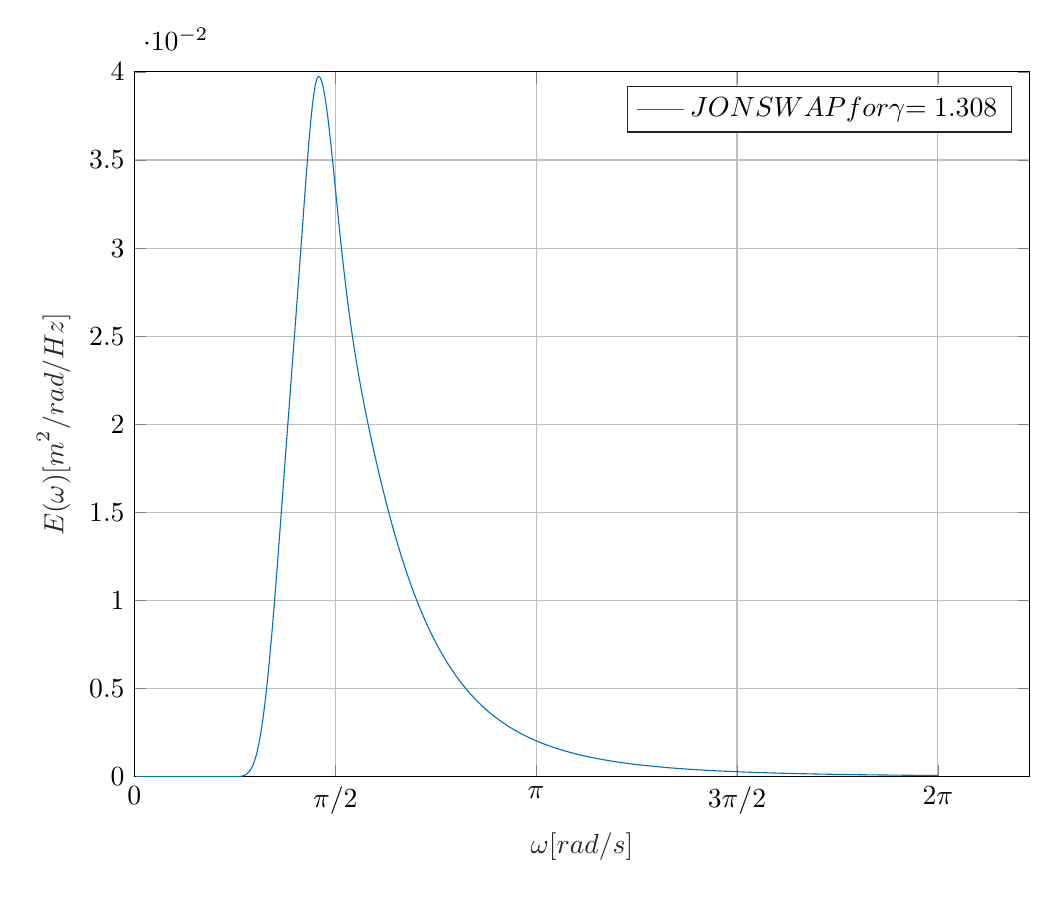
\begin{tikzpicture}

\begin{axis}[%
width=4.476in,
height=3.524in,
at={(0.803in,0.523in)},
scale only axis,
unbounded coords=jump,
xmin=0,
xmax=7,
xtick={0,1.5707963267949,3.14159265358979,4.71238898038469,6.28318530717959},
xticklabels={{0},{$\pi\text{/2}$},{$\pi$},{$\text{3}\pi\text{/2}$},{$\text{2}\pi$}},
xlabel style={font=\color{white!15!black}},
xlabel={$\omega\text{ [rad/s]}$},
ymin=0,
ymax=0.04,
ylabel style={font=\color{white!15!black}},
ylabel={$\text{E(}\omega\text{) [m}^\text{2}\text{/rad/Hz]}$},
axis background/.style={fill=white},
title style={font=\bfseries},
%title={$\text{One-dimensional wave spectrum, E(}\omega\text{) at -34S, 17.25E}$},
xmajorgrids,
ymajorgrids,
legend style={legend cell align=left, align=left, draw=white!15!black}
]
\addplot [color=mycolor1]
  table[row sep=crcr]{%
0	nan\\
0.0122958616578857	0\\
0.0245917233157714	0\\
0.0368875849736571	0\\
0.0491834466315427	0\\
0.0614793082894284	0\\
0.0737751699473141	0\\
0.0860710316051998	0\\
0.0983668932630855	0\\
0.110662754920971	0\\
0.122958616578857	0\\
0.135254478236743	0\\
0.147550339894628	0\\
0.159846201552514	0\\
0.1721420632104	0\\
0.184437924868285	0\\
0.196733786526171	0\\
0.209029648184057	0\\
0.221325509841942	0\\
0.233621371499828	0\\
0.245917233157714	0\\
0.258213094815599	0\\
0.270508956473485	0\\
0.282804818131371	0\\
0.295100679789256	5.41302879763333e-307\\
0.307396541447142	1.4351658983951e-260\\
0.319692403105028	1.39801651640755e-222\\
0.331988264762914	2.95955173493782e-191\\
0.344284126420799	3.06617261869068e-165\\
0.356579988078685	1.71585454184354e-143\\
0.368875849736571	3.36115162791715e-125\\
0.381171711394456	9.99471845091621e-110\\
0.393467573052342	1.44074967318733e-96\\
0.405763434710228	2.54134308132756e-85\\
0.418059296368113	1.15384979645612e-75\\
0.430355158025999	2.46010694641464e-67\\
0.442651019683885	4.01707121559874e-60\\
0.45494688134177	7.49671131280128e-54\\
0.467242742999656	2.22288404307939e-48\\
0.479538604657542	1.3753760835859e-43\\
0.491834466315427	2.22745866619101e-39\\
0.504130327973313	1.14105811314078e-35\\
0.516426189631199	2.16730148431401e-32\\
0.528722051289085	1.74501685936915e-29\\
0.54101791294697	6.67054290550385e-27\\
0.553313774604856	1.33294088654399e-24\\
0.565609636262742	1.51145852287043e-22\\
0.577905497920627	1.0433270916913e-20\\
0.590201359578513	4.65664898554377e-19\\
0.602497221236399	1.41551545559892e-17\\
0.614793082894284	3.06504085545376e-16\\
0.62708894455217	4.91508596715723e-15\\
0.639384806210056	6.03782647089776e-14\\
0.651680667867941	5.85166582657271e-13\\
0.663976529525827	4.59100381164424e-12\\
0.676272391183713	2.98235025750544e-11\\
0.688568252841599	1.63618607596188e-10\\
0.700864114499484	7.71435740175365e-10\\
0.71315997615737	3.17422780050511e-09\\
0.725455837815256	1.15545266932238e-08\\
0.737751699473141	3.76593918002615e-08\\
0.750047561131027	1.11082567474578e-07\\
0.762343422788913	2.99365257438456e-07\\
0.774639284446798	7.43398794457705e-07\\
0.786935146104684	1.71393732492197e-06\\
0.79923100776257	3.6936978163335e-06\\
0.811526869420455	7.48610717182671e-06\\
0.823822731078341	1.43464290828625e-05\\
0.836118592736227	2.61246562604755e-05\\
0.848414454394112	4.54036148623333e-05\\
0.860710316051998	7.56117606150625e-05\\
0.873006177709884	0.000121089372916668\\
0.88530203936777	0.000187089786772187\\
0.897597901025655	0.000279703606526386\\
0.909893762683541	0.000405702450085907\\
0.922189624341426	0.000572308176547121\\
0.934485485999312	0.000786902195884214\\
0.946781347657198	0.00105669606424971\\
0.959077209315084	0.00138838834019309\\
0.971373070972969	0.00178783338397504\\
0.983668932630855	0.00225974569705202\\
0.995964794288741	0.00280745915996462\\
1.00826065594663	0.00343275496464683\\
1.02055651760451	0.00413576600873186\\
1.0328523792624	0.00491495977802167\\
1.04514824092028	0.00576719685342651\\
1.05744410257817	0.00668785847600663\\
1.06973996423605	0.00767103419145496\\
1.08203582589394	0.00870975936699404\\
1.09433168755183	0.0097962920536587\\
1.10662754920971	0.0109224188636112\\
1.1189234108676	0.0120797798007726\\
1.13121927252548	0.0132602018978306\\
1.14351513418337	0.0144560307440969\\
1.15581099584125	0.0156604473784329\\
1.16810685749914	0.0168677556407375\\
1.18040271915703	0.0180736222488931\\
1.19269858081491	0.0192752491472963\\
1.2049944424728	0.0204714557558278\\
1.21729030413068	0.0216626483564445\\
1.22958616578857	0.0228506556097147\\
1.24188202744645	0.0240384135360737\\
1.25417788910434	0.0252294904939306\\
1.26647375076223	0.0264274529344006\\
1.27876961242011	0.0276350862726403\\
1.291065474078	0.0288535024756524\\
1.30336133573588	0.0300811872588852\\
1.31565719739377	0.0313130648442189\\
1.32795305905165	0.0325396852882558\\
1.34024892070954	0.0337466641153829\\
1.35254478236743	0.0349145188355605\\
1.36484064402531	0.0360190415875961\\
1.3771365056832	0.0370323108877261\\
1.38943236734108	0.0379243714742074\\
1.40172822899897	0.0386655021114703\\
1.41402409065685	0.0392288631897149\\
1.42631995231474	0.0395931988386078\\
1.43861581397263	0.0397451987880671\\
1.45091167563051	0.0397009837064543\\
1.4632075372884	0.0395060933162202\\
1.47550339894628	0.0391703952648501\\
1.48779926060417	0.0387059506556059\\
1.50009512226205	0.0381276193041899\\
1.51239098391994	0.0374522472133023\\
1.52468684557783	0.0366977905296433\\
1.53698270723571	0.0358824534634019\\
1.5492785688936	0.0350239067515314\\
1.56157443055148	0.0341386357865274\\
1.57387029220937	0.033241447182027\\
1.58616615386725	0.0323451427488864\\
1.59846201552514	0.0314603532066003\\
1.61075787718303	0.0305955119179262\\
1.62305373884091	0.0297569418708591\\
1.6353496004988	0.0289490265523619\\
1.64764546215668	0.0281744362672717\\
1.65994132381457	0.0274343846835443\\
1.67223718547245	0.0267288948374096\\
1.68453304713034	0.0260570586376697\\
1.69682890878822	0.0254172784703886\\
1.70912477044611	0.0248074834845985\\
1.721420632104	0.024225316400738\\
1.73371649376188	0.023668289227364\\
1.74601235541977	0.0231339081746281\\
1.75830821707765	0.0226197694201764\\
1.77060407873554	0.0221236283185714\\
1.78289994039342	0.0216434452374737\\
1.79519580205131	0.0211774115218765\\
1.8074916637092	0.0207239591846428\\
1.81978752536708	0.0202817578397189\\
1.83208338702497	0.0198497021705522\\
1.84437924868285	0.0194268928954684\\
1.85667511034074	0.0190126137886203\\
1.86897097199862	0.0186063068732881\\
1.88126683365651	0.0182075474549375\\
1.8935626953144	0.0178160202313337\\
1.90585855697228	0.0174314973270267\\
1.91815441863017	0.0170538187637728\\
1.93045028028805	0.0166828756042898\\
1.94274614194594	0.0163185957954444\\
1.95504200360382	0.0159609325850235\\
1.96733786526171	0.0156098552867384\\
1.9796337269196	0.015265342112225\\
1.99192958857748	0.0149273747670556\\
2.00422545023537	0.0145959345109985\\
2.01652131189325	0.0142709994027779\\
2.02881717355114	0.0139525424796016\\
2.04111303520902	0.0136405306563983\\
2.05340889686691	0.0133349241651845\\
2.0657047585248	0.0130356763886258\\
2.07800062018268	0.0127427339721329\\
2.09029648184057	0.0124560371249502\\
2.10259234349845	0.0121755200424896\\
2.11488820515634	0.0119011113998192\\
2.12718406681422	0.0116327348801607\\
2.13947992847211	0.011370309712995\\
2.15177579012999	0.0111137512044894\\
2.16407165178788	0.0108629712489418\\
2.17636751344577	0.0106178788142673\\
2.18866337510365	0.0103783803976124\\
2.20095923676154	0.0101443804493013\\
2.21325509841942	0.00991578176473845\\
2.22555096007731	0.00969248584482827\\
2.2378468217352	0.00947439322604724\\
2.25014268339308	0.00926140378164897\\
2.26243854505097	0.0090534169956585\\
2.27473440670885	0.00885033221138453\\
2.28703026836674	0.00865204885617913\\
2.29932613002462	0.00845846664413426\\
2.31162199168251	0.00826948575833719\\
2.3239178533404	0.00808500701422663\\
2.33621371499828	0.00790493200550391\\
2.34850957665617	0.00772916323396475\\
2.36080543831405	0.00755760422452847\\
2.37310129997194	0.00739015962665654\\
2.38539716162982	0.00722673530327022\\
2.39769302328771	0.00706723840819925\\
2.40998888494559	0.00691157745312068\\
2.42228474660348	0.0067596623648772\\
2.43458060826137	0.00661140453400037\\
2.44687646991925	0.00646671685520286\\
2.45917233157714	0.00632551376054758\\
2.47146819323502	0.00618771124594853\\
2.48376405489291	0.00605322689160874\\
2.49605991655079	0.00592197987695489\\
2.50835577820868	0.00579389099058502\\
2.52065163986657	0.00566888263570622\\
2.53294750152445	0.00554687883150177\\
2.54524336318234	0.00542780521083287\\
2.55753922484022	0.00531158901464808\\
2.56983508649811	0.00519815908344373\\
2.58213094815599	0.00508744584609102\\
2.59442680981388	0.00497938130631981\\
2.60672267147177	0.00487389902712567\\
2.61901853312965	0.00477093411334424\\
2.63131439478754	0.00467042319261705\\
2.64361025644542	0.00457230439495386\\
2.65590611810331	0.00447651733107909\\
2.66820197976119	0.00438300306973388\\
2.68049784141908	0.00429170411409041\\
2.69279370307697	0.00420256437742111\\
2.70508956473485	0.00411552915815301\\
2.71738542639274	0.00403054511442532\\
2.72968128805062	0.00394756023825787\\
2.74197714970851	0.00386652382942774\\
2.75427301136639	0.00378738646914243\\
2.76656887302428	0.00371009999358922\\
2.77886473468217	0.00363461746743274\\
2.79116059634005	0.00356089315732546\\
2.80345645799794	0.00348888250548924\\
2.81575231965582	0.00341854210342006\\
2.82804818131371	0.00334982966576232\\
2.84034404297159	0.00328270400439414\\
2.85263990462948	0.00321712500276036\\
2.86493576628737	0.00315305359048552\\
2.87723162794525	0.00309045171829528\\
2.88952748960314	0.00302928233327117\\
2.90182335126102	0.0029695093544601\\
2.91411921291891	0.00291109764885714\\
2.92641507457679	0.00285401300777748\\
2.93871093623468	0.00279822212363068\\
2.95100679789256	0.00274369256710825\\
2.96330265955045	0.00269039276479353\\
2.97559852120834	0.00263829197720089\\
2.98789438286622	0.00258736027724954\\
3.00019024452411	0.00253756852917576\\
3.01248610618199	0.00248888836788607\\
3.02478196783988	0.00244129217875227\\
3.03707782949776	0.00239475307784859\\
3.04937369115565	0.00234924489262979\\
3.06166955281354	0.0023047421430484\\
3.07396541447142	0.0022612200231083\\
3.08626127612931	0.00221865438285134\\
3.09855713778719	0.00217702171077273\\
3.11085299944508	0.00213629911666074\\
3.12314886110296	0.00209646431485547\\
3.13544472276085	0.00205749560792113\\
3.14774058441874	0.00201937187072593\\
3.16003644607662	0.00198207253492326\\
3.17233230773451	0.00194557757382764\\
3.18462816939239	0.00190986748767868\\
3.19692403105028	0.00187492328928602\\
3.20921989270816	0.00184072649004824\\
3.22151575436605	0.00180725908633834\\
3.23381161602394	0.00177450354624858\\
3.24610747768182	0.00174244279668723\\
3.25840333933971	0.00171106021081969\\
3.27069920099759	0.0016803395958467\\
3.28299506265548	0.00165026518111192\\
3.29529092431336	0.00162082160653164\\
3.30758678597125	0.00159199391133908\\
3.31988264762914	0.00156376752313587\\
3.33217850928702	0.00153612824724346\\
3.34447437094491	0.00150906225634721\\
3.35677023260279	0.00148255608042589\\
3.36906609426068	0.00145659659695957\\
3.38136195591856	0.00143117102140895\\
3.39365781757645	0.00140626689795909\\
3.40595367923434	0.00138187209052092\\
3.41824954089222	0.00135797477398379\\
3.43054540255011	0.00133456342571239\\
3.44284126420799	0.00131162681728186\\
3.45513712586588	0.00128915400644448\\
3.46743298752376	0.00126713432932197\\
3.47972884918165	0.00124555739281723\\
3.49202471083954	0.00122441306723957\\
3.50432057249742	0.00120369147913769\\
3.51661643415531	0.00118338300433464\\
3.52891229581319	0.00116347826115928\\
3.54120815747108	0.00114396810386871\\
3.55350401912896	0.00112484361625655\\
3.56579988078685	0.0011060961054416\\
3.57809574244473	0.00108771709583218\\
3.59039160410262	0.00106969832326091\\
3.60268746576051	0.00105203172928534\\
3.61498332741839	0.00103470945564963\\
3.62727918907628	0.0010177238389028\\
3.63957505073416	0.00100106740516895\\
3.65187091239205	0.000984732865065375\\
3.66416677404994	0.000968713108764074\\
3.67646263570782	0.00095300120119279\\
3.68875849736571	0.00093759037737141\\
3.70105435902359	0.000922474037879949\\
3.71335022068148	0.000907645744454282\\
3.72564608233936	0.000893099215705966\\
3.73794194399725	0.000878828322962575\\
3.75023780565513	0.000864827086225059\\
3.76253366731302	0.000851089670238769\\
3.77482952897091	0.000837610380674829\\
3.78712539062879	0.000824383660418703\\
3.79942125228668	0.000811404085962812\\
3.81171711394456	0.00079866636390022\\
3.82401297560245	0.000786165327516438\\
3.83630883726033	0.000773895933476511\\
3.84860469891822	0.000761853258604621\\
3.86090056057611	0.000750032496753526\\
3.87319642223399	0.000738428955761214\\
3.88549228389188	0.000727038054492271\\
3.89778814554976	0.000715855319961465\\
3.91008400720765	0.000704876384537197\\
3.92237986886553	0.000694096983222478\\
3.93467573052342	0.000683512951011199\\
3.94697159218131	0.000673120220317491\\
3.95926745383919	0.000662914818476088\\
3.97156331549708	0.000652892865311599\\
3.98385917715496	0.000643050570774724\\
3.99615503881285	0.000633384232643455\\
4.00845090047073	0.000623890234287399\\
4.02074676212862	0.000614565042493382\\
4.03304262378651	0.000605405205350579\\
4.04533848544439	0.000596407350193436\\
4.05763434710228	0.000587568181600735\\
4.06993020876016	0.000578884479449159\\
4.08222607041805	0.00057035309701982\\
4.09452193207593	0.000561970959156189\\
4.10681779373382	0.000553735060471986\\
4.1191136553917	0.000545642463607562\\
4.13140951704959	0.000537690297533413\\
4.14370537870748	0.00052987575589945\\
4.15600124036536	0.000522196095428724\\
4.16829710202325	0.000514648634354346\\
4.18059296368113	0.00050723075089834\\
4.19288882533902	0.00049993988179127\\
4.2051846869969	0.000492773520831441\\
4.21748054865479	0.00048572921748257\\
4.22977641031268	0.000478804575508837\\
4.24207227197056	0.000471997251646233\\
4.25436813362845	0.000465304954309197\\
4.26666399528633	0.000458725442331523\\
4.27895985694422	0.000452256523740597\\
4.29125571860211	0.000445896054563984\\
4.30355158025999	0.000439641937667487\\
4.31584744191788	0.000433492121623766\\
4.32814330357576	0.000427444599610678\\
4.34043916523365	0.000421497408338488\\
4.35273502689153	0.000415648627005148\\
4.36503088854942	0.000409896376278856\\
4.37732675020731	0.000404238817307136\\
4.38962261186519	0.000398674150751693\\
4.40191847352308	0.000393200615848326\\
4.41421433518096	0.000387816489491206\\
4.42651019683885	0.000382520085340833\\
4.43880605849673	0.000377309752955029\\
4.45110192015462	0.000372183876942308\\
4.46339778181251	0.000367140876137024\\
4.47569364347039	0.000362179202795692\\
4.48798950512828	0.000357297341813879\\
4.50028536678616	0.000352493809963128\\
4.51258122844405	0.000347767155147345\\
4.52487709010193	0.000343115955678117\\
4.53717295175982	0.000338538819568452\\
4.5494688134177	0.000334034383844427\\
4.56176467507559	0.000329601313874257\\
4.57406053673348	0.000325238302714321\\
4.58635639839136	0.000320944070471665\\
4.59865226004925	0.000316717363682552\\
4.61094812170713	0.000312556954706612\\
4.62324398336502	0.00030846164113618\\
4.6355398450229	0.000304430245220401\\
4.64783570668079	0.000300461613303707\\
4.66013156833868	0.000296554615278295\\
4.67242742999656	0.000292708144050196\\
4.68472329165445	0.000288921115018604\\
4.69701915331233	0.000285192465568094\\
4.70931501497022	0.000281521154573383\\
4.7216108766281	0.000277906161916305\\
4.73390673828599	0.000274346488014674\\
4.74620259994388	0.000270841153362717\\
4.75849846160176	0.000267389198082769\\
4.77079432325965	0.000263989681487935\\
4.78309018491753	0.000260641681655428\\
4.79538604657542	0.000257344295010299\\
4.8076819082333	0.000254096635919287\\
4.81997776989119	0.000250897836294526\\
4.83227363154908	0.000247747045206839\\
4.84456949320696	0.000244643428508389\\
4.85686535486485	0.000241586168464416\\
4.86916121652273	0.000238574463393844\\
4.88145707818062	0.000235607527318515\\
4.8937529398385	0.000232684589620834\\
4.90604880149639	0.000229804894709597\\
4.91834466315427	0.000226967701693801\\
4.93064052481216	0.000224172284064218\\
4.94293638647005	0.000221417929382543\\
4.95523224812793	0.000218703938977918\\
4.96752810978582	0.000216029627650631\\
4.9798239714437	0.000213394323382829\\
4.99211983310159	0.000210797367056043\\
5.00441569475948	0.000208238112175362\\
5.01671155641736	0.000205715924600084\\
5.02900741807525	0.000203230182280682\\
5.04130327973313	0.000200780275001916\\
5.05359914139102	0.000198365604131947\\
5.0658950030489	0.000195985582377289\\
5.07819086470679	0.00019363963354346\\
5.09048672636467	0.000191327192301187\\
5.10278258802256	0.000189047703958018\\
5.11507844968045	0.000186800624235214\\
5.12737431133833	0.00018458541904979\\
5.13967017299622	0.000182401564301559\\
5.1519660346541	0.000180248545665076\\
5.16426189631199	0.000178125858386348\\
5.17655775796987	0.000176033007084189\\
5.18885361962776	0.000173969505556115\\
5.20114948128565	0.000171934876588657\\
5.21344534294353	0.000169928651771981\\
5.22574120460142	0.000167950371318724\\
5.2380370662593	0.000165999583886923\\
5.25033292791719	0.000164075846406948\\
5.26262878957507	0.000162178723912337\\
5.27492465123296	0.000160307789374435\\
5.28722051289085	0.000158462623540752\\
5.29951637454873	0.000156642814776941\\
5.31181223620662	0.000154847958912307\\
5.3241080978645	0.000153077659088771\\
5.33640395952239	0.000151331525613192\\
5.34869982118027	0.000149609175812981\\
5.36099568283816	0.000147910233894908\\
5.37329154449605	0.000146234330807043\\
5.38558740615393	0.000144581104103749\\
5.39788326781182	0.000142950197813643\\
5.4101791294697	0.000141341262310475\\
5.42247499112759	0.000139753954186838\\
5.43477085278547	0.000138187936130644\\
5.44706671444336	0.000136642876804307\\
5.45936257610125	0.000135118450726565\\
5.47165843775913	0.000133614338156872\\
5.48395429941702	0.00013213022498231\\
5.4962501610749	0.00013066580260695\\
5.50854602273279	0.000129220767843618\\
5.52084188439067	0.000127794822807993\\
5.53313774604856	0.000126387674814993\\
5.54543360770645	0.000124999036277395\\
5.55772946936433	0.000123628624606628\\
5.57002533102222	0.000122276162115703\\
5.5823211926801	0.00012094137592421\\
5.59461705433799	0.000119623997865353\\
5.60691291599587	0.000118323764394966\\
5.61920877765376	0.00011704041650246\\
5.63150463931164	0.000115773699623671\\
5.64380050096953	0.000114523363555545\\
5.65609636262742	0.000113289162372638\\
5.6683922242853	0.00011207085434537\\
5.68068808594319	0.000110868201860007\\
5.69298394760107	0.000109680971340328\\
5.70527980925896	0.00010850893317093\\
5.71757567091684	0.000107351861622146\\
5.72987153257473	0.000106209534776526\\
5.74216739423262	0.000105081734456864\\
5.7544632558905	0.000103968246155711\\
5.76675911754839	0.000102868858966361\\
5.77905497920627	0.000101783365515268\\
5.79135084086416	0.000100711561895862\\
5.80364670252204	9.96532476037344e-05\\
5.81594256417993	9.86082254731543e-05\\
5.82823842583782	9.75763016149018e-05\\
5.8405342874957	9.65572853553714e-05\\
5.85283014915359	9.55509891769276e-05\\
5.86512601081147	9.455722865948e-05\\
5.87742187246936	9.35758224232536e-05\\
5.88971773412724	9.26065920727251e-05\\
5.90201359578513	9.16493621417014e-05\\
5.91430945744302	9.07039600395125e-05\\
5.9266053191009	8.97702159982964e-05\\
5.93890118075879	8.88479630213512e-05\\
5.95119704241667	8.79370368325295e-05\\
5.96349290407456	8.70372758266536e-05\\
5.97578876573244	8.61485210209284e-05\\
5.98808462739033	8.5270616007331e-05\\
6.00038048904822	8.4403406905953e-05\\
6.0126763507061	8.35467423192785e-05\\
6.02497221236399	8.27004732873734e-05\\
6.03726807402187	8.18644532439695e-05\\
6.04956393567976	8.10385379734214e-05\\
6.06185979733764	8.02225855685183e-05\\
6.07415565899553	7.94164563891332e-05\\
6.08645152065342	7.86200130216882e-05\\
6.0987473823113	7.78331202394225e-05\\
6.11104324396919	7.70556449634419e-05\\
6.12333910562707	7.62874562245356e-05\\
6.13563496728496	7.55284251257423e-05\\
6.14793082894284	7.4778424805651e-05\\
6.16022669060073	7.40373304024179e-05\\
6.17252255225862	7.33050190184887e-05\\
6.1848184139165	7.25813696860062e-05\\
6.19711427557439	7.18662633328921e-05\\
6.20941013723227	7.11595827495877e-05\\
6.22170599889016	7.04612125564384e-05\\
6.23400186054804	6.97710391717103e-05\\
6.24629772220593	6.90889507802242e-05\\
6.25859358386381	6.84148373025936e-05\\
6.2708894455217	6.77485903650559e-05\\
6.28318530717959	6.70901032698821e-05\\
};
\addlegendentry{$\text{JONSWAP for }\gamma\text{ = 1.308}$}

\end{axis}
\end{tikzpicture}%}
    }
    \subcaptionbox{\acs{jonswap} spectrum at multiple geographical locations\label{fig:systemDesign.1DSampleWaveSpectrumMultiple}}[0.48\linewidth]{
        \resizebox{\linewidth}{!}{% This file was created by matlab2tikz.
%
%The latest updates can be retrieved from
%  http://www.mathworks.com/matlabcentral/fileexchange/22022-matlab2tikz-matlab2tikz
%where you can also make suggestions and rate matlab2tikz.
%
\definecolor{mycolor1}{rgb}{0.00000,0.44700,0.74100}%
\definecolor{mycolor2}{rgb}{0.85000,0.32500,0.09800}%
\definecolor{mycolor3}{rgb}{0.92900,0.69400,0.12500}%
%
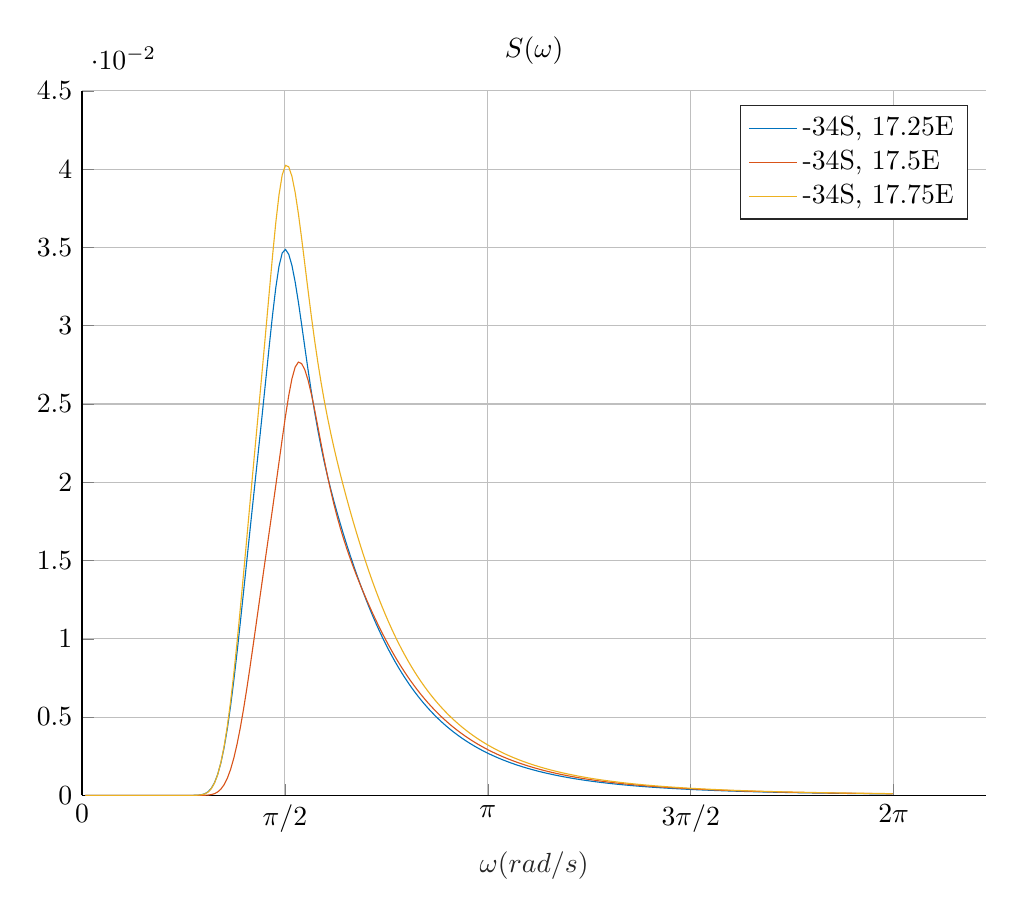
\begin{tikzpicture}

\begin{axis}[%
width=4.521in,
height=3.522in,
at={(0.758in,0.525in)},
scale only axis,
unbounded coords=jump,
xmin=0,
xmax=7,
xtick={0,1.5707963267949,3.14159265358979,4.71238898038469,6.28318530717959},
xticklabels={{0},{$\pi\text{/2}$},{$\pi$},{$\text{3}\pi\text{/2}$},{$\text{2}\pi$}},
xlabel style={font=\color{white!15!black}},
xlabel={$\omega\text{ (rad/s)}$},
ymin=0,
ymax=0.045,
axis background/.style={fill=white},
title style={font=\bfseries},
title={$\text{S(}\omega\text{)}$},
axis x line*=bottom,
axis y line*=left,
xmajorgrids,
ymajorgrids,
legend style={legend cell align=left, align=left, draw=white!15!black}
]
\addplot [color=mycolor1]
  table[row sep=crcr]{%
0	nan\\
0.025	0\\
0.05	0\\
0.075	0\\
0.1	0\\
0.125	0\\
0.15	0\\
0.175	0\\
0.2	0\\
0.225	0\\
0.25	0\\
0.275	0\\
0.3	0\\
0.325	1.42005336164696e-294\\
0.35	9.69071650364021e-219\\
0.375	8.9429723835081e-166\\
0.4	6.86905098134045e-128\\
0.425	3.20255852046391e-100\\
0.45	1.21756251134366e-79\\
0.475	4.39413653830271e-64\\
0.5	3.75253612752824e-52\\
0.525	6.98108061469795e-43\\
0.55	1.34803558535101e-35\\
0.575	8.25367875478129e-30\\
0.6	3.60599202847064e-25\\
0.625	2.04313512836628e-21\\
0.65	2.34443210340736e-18\\
0.675	7.62728076531269e-16\\
0.7	9.0949466938071e-14\\
0.725	4.84481568023764e-12\\
0.75	1.34483165611122e-10\\
0.775	2.19505591732068e-09\\
0.8	2.318044183753e-08\\
0.825	1.70916497388674e-07\\
0.85	9.35389155141354e-07\\
0.875	3.992162425786e-06\\
0.9	1.3831886598667e-05\\
0.925	4.02052989185634e-05\\
0.95	0.000100727994773396\\
0.975	0.000222425310970658\\
1	0.000441006963165027\\
1.025	0.000797372567629214\\
1.05	0.00133190077564372\\
1.075	0.00207790756217197\\
1.1	0.0030559080662334\\
1.125	0.00426997806642068\\
1.15	0.00570684818691764\\
1.175	0.00733769741253571\\
1.2	0.00912215841757366\\
1.225	0.0110138541085512\\
1.25	0.0129667569467849\\
1.275	0.0149416351893377\\
1.3	0.0169116910403878\\
1.325	0.0188662030491418\\
1.35	0.0208107258820418\\
1.375	0.0227624442046733\\
1.4	0.024739866260253\\
1.425	0.0267473331406231\\
1.45	0.0287569318401041\\
1.475	0.0306932991380638\\
1.5	0.0324296209170312\\
1.525	0.0338033021382225\\
1.55	0.0346538234111679\\
1.575	0.0348755540522296\\
1.6	0.034570350289043\\
1.625	0.0338501254944236\\
1.65	0.0327954806171921\\
1.675	0.0315056626382637\\
1.7	0.0300819498206769\\
1.725	0.0286138559462538\\
1.75	0.0271707317717678\\
1.775	0.0257990589714608\\
1.8	0.0245241456527203\\
1.825	0.023354359682383\\
1.85	0.0222862257976691\\
1.875	0.0213092374401057\\
1.9	0.0204097709626139\\
1.925	0.0195738934373654\\
1.95	0.0187891077675736\\
1.975	0.0180452135986114\\
2	0.017334517187952\\
2.025	0.0166516250019896\\
2.05	0.0159930233551372\\
2.075	0.0153565957251796\\
2.1	0.0147411745392796\\
2.125	0.0141461760752534\\
2.15	0.0135713317070127\\
2.175	0.0130165072391482\\
2.2	0.0124815922977106\\
2.225	0.0119664399539165\\
2.25	0.0114708393086541\\
2.275	0.0109945079204131\\
2.3	0.0105370950733649\\
2.325	0.0100981902094815\\
2.35	0.00967733322006807\\
2.375	0.00927402482938858\\
2.4	0.00888773622319186\\
2.425	0.00851791758658041\\
2.45	0.00816400547937364\\
2.475	0.00782542910107779\\
2.5	0.00750161554792925\\
2.525	0.00719199417862887\\
2.55	0.00689600020308854\\
2.575	0.00661307759957541\\
2.6	0.00634268145463997\\
2.625	0.00608427980914861\\
2.65	0.00583735508339847\\
2.675	0.00560140514493138\\
2.7	0.00537594407431956\\
2.725	0.00516050267681694\\
2.75	0.00495462878127661\\
2.775	0.00475788736203881\\
2.8	0.00456986051451048\\
2.825	0.00439014731080689\\
2.85	0.00421836355803606\\
2.875	0.00405414147851078\\
2.9	0.00389712932831215\\
2.925	0.00374699096814987\\
2.95	0.00360340539831963\\
2.975	0.00346606626770631\\
3	0.00333468136518456\\
3.025	0.00320897210039438\\
3.05	0.00308867297968838\\
3.075	0.00297353108203495\\
3.1	0.00286330553879531\\
3.125	0.0027577670205521\\
3.15	0.00265669723353696\\
3.175	0.00255988842766866\\
3.2	0.00246714291775922\\
3.225	0.00237827261906212\\
3.25	0.0022930985980135\\
3.275	0.0022114506387469\\
3.3	0.00213316682573592\\
3.325	0.002058093142732\\
3.35	0.00198608308800986\\
3.375	0.00191699730580667\\
3.4	0.00185070323373864\\
3.425	0.0017870747658966\\
3.45	0.00172599193125724\\
3.475	0.0016673405869969\\
3.5	0.00161101212625658\\
3.525	0.00155690319987984\\
3.55	0.00150491545162645\\
3.575	0.00145495526635325\\
3.6	0.00140693353064837\\
3.625	0.00136076540540445\\
3.65	0.00131637010982037\\
3.675	0.00127367071632743\\
3.7	0.00123259395594611\\
3.725	0.00119307003359064\\
3.75	0.00115503245285207\\
3.775	0.00111841784980484\\
3.8	0.00108316583539729\\
3.825	0.00104921884600218\\
3.85	0.00101652200171983\\
3.875	0.000985022972042542\\
3.9	0.000954671848505669\\
3.925	0.000925421023966832\\
3.95	0.000897225078170812\\
3.975	0.000870040669273467\\
4	0.000843826431013326\\
4.025	0.000818542875234467\\
4.05	0.000794152299478739\\
4.075	0.000770618699379366\\
4.1	0.000747907685601413\\
4.125	0.00072598640508757\\
4.15	0.000704823466380049\\
4.175	0.000684388868801333\\
4.2	0.000664653935287829\\
4.225	0.000645591248681324\\
4.25	0.000627174591293489\\
4.275	0.000609378887568506\\
4.3	0.000592180149678229\\
4.325	0.000575555425893253\\
4.35	0.000559482751581628\\
4.375	0.000543941102695051\\
4.4	0.000528910351609916\\
4.425	0.000514371225197852\\
4.45	0.00050030526500717\\
4.475	0.000486694789443137\\
4.5	0.000473522857841097\\
4.525	0.000460773236332246\\
4.55	0.000448430365407371\\
4.575	0.000436479329088995\\
4.6	0.000424905825627315\\
4.625	0.000413696139639911\\
4.65	0.000402837115619594\\
4.675	0.00039231613273888\\
4.7	0.000382121080883498\\
4.725	0.000372240337850987\\
4.75	0.000362662747653968\\
4.775	0.000353377599870921\\
4.8	0.000344374609990426\\
4.825	0.000335643900697739\\
4.85	0.00032717598405536\\
4.875	0.000318961744531857\\
4.9	0.00031099242283565\\
4.925	0.00030325960051285\\
4.95	0.000295755185270374\\
4.975	0.000288471396987688\\
5	0.000281400754382471\\
5.025	0.000274536062297339\\
5.05	0.000267870399576535\\
5.075	0.000261397107503122\\
5.1	0.000255109778768796\\
5.125	0.000249002246949895\\
5.15	0.00024306857646458\\
5.175	0.00023730305298748\\
5.2	0.000231700174299331\\
5.225	0.000226254641550318\\
5.25	0.000220961350916936\\
5.275	0.000215815385633239\\
5.3	0.000210812008378337\\
5.325	0.000205946654002934\\
5.35	0.00020121492257859\\
5.375	0.000196612572754239\\
5.4	0.000192135515405258\\
5.425	0.000187779807561172\\
5.45	0.000183541646598761\\
5.475	0.000179417364688014\\
5.5	0.00017540342347901\\
5.525	0.000171496409018418\\
5.55	0.000167693026884859\\
5.575	0.000163990097532923\\
5.6	0.000160384551836145\\
5.625	0.000156873426819724\\
5.65	0.000153453861574227\\
5.675	0.000150123093341946\\
5.7	0.000146878453768014\\
5.725	0.000143717365308734\\
5.75	0.000140637337789977\\
5.775	0.000137635965108847\\
5.8	0.000134710922072129\\
5.825	0.000131859961365367\\
5.85	0.000129080910646709\\
5.875	0.000126371669759938\\
5.9	0.000123730208061383\\
5.925	0.000121154561855647\\
5.95	0.000118642831935349\\
5.975	0.000116193181220273\\
6	0.000113803832491587\\
6.025	0.000111473066216942\\
6.05	0.000109199218462497\\
6.075	0.0001069806788881\\
6.1	0.000104815888822006\\
6.125	0.00010270333941171\\
6.15	0.00010064156984762\\
6.175	9.86291656564363e-05\\
6.2	9.6664757061278e-05\\
6.225	9.47470174056977e-05\\
6.25	9.28746616388853e-05\\
6.275	9.10464448594679e-05\\
};
\addlegendentry{-34S, 17.25E}

\addplot [color=mycolor2]
  table[row sep=crcr]{%
0	nan\\
0.025	0\\
0.05	0\\
0.075	0\\
0.1	0\\
0.125	0\\
0.15	0\\
0.175	0\\
0.2	0\\
0.225	0\\
0.25	0\\
0.275	0\\
0.3	0\\
0.325	0\\
0.35	1.26023267647914e-286\\
0.375	2.80742285912933e-217\\
0.4	1.15423998900674e-167\\
0.425	2.02107405553599e-131\\
0.45	1.86868682798001e-104\\
0.475	4.60933261613972e-84\\
0.5	2.03972418249546e-68\\
0.525	2.95770419372233e-56\\
0.55	1.08420372141137e-46\\
0.575	4.33261982135442e-39\\
0.6	5.456411602635e-33\\
0.625	4.73344201009094e-28\\
0.65	5.06909418436034e-24\\
0.675	1.04097764795055e-20\\
0.7	5.73696575837785e-18\\
0.725	1.09945034203276e-15\\
0.75	8.96335746326885e-14\\
0.775	3.64148162149331e-12\\
0.8	8.35526718958735e-11\\
0.825	1.19633700827992e-09\\
0.85	1.15810736686838e-08\\
0.875	8.08654278258996e-08\\
0.9	4.29299536041855e-07\\
0.925	1.80902487165885e-06\\
0.95	6.26901238836794e-06\\
0.975	1.83968816376402e-05\\
1	4.68435036975908e-05\\
1.025	0.000105618141111768\\
1.05	0.000214491975607496\\
1.075	0.00039801373348157\\
1.1	0.000683074350356013\\
1.125	0.00109544992319851\\
1.15	0.00165608058393325\\
1.175	0.00237789566863525\\
1.2	0.00326380259088047\\
1.225	0.00430613787663511\\
1.25	0.00548756612480977\\
1.275	0.00678319436113273\\
1.3	0.00816356824501939\\
1.325	0.00959819824379329\\
1.35	0.0110592615026501\\
1.375	0.0125250754399833\\
1.4	0.0139828198446664\\
1.425	0.0154298383453943\\
1.45	0.0168727769517118\\
1.475	0.0183239297541959\\
1.5	0.0197945427154998\\
1.525	0.0212855292348837\\
1.55	0.0227771232238175\\
1.575	0.024220397078593\\
1.6	0.025534878235119\\
1.625	0.0266165814609852\\
1.65	0.0273581368724443\\
1.675	0.0276770000818049\\
1.7	0.0275833999522577\\
1.725	0.0271818788239301\\
1.75	0.0265186664780573\\
1.775	0.0256534183300569\\
1.8	0.0246525017591413\\
1.825	0.0235799191422533\\
1.85	0.0224904397870587\\
1.875	0.0214258032666902\\
1.9	0.0204138477111174\\
1.925	0.0194697984451437\\
1.95	0.018598775052583\\
1.975	0.0177987019024249\\
2	0.0170630604722376\\
2.025	0.0163831735039183\\
2.05	0.0157499034661201\\
2.075	0.0151547729166714\\
2.1	0.014590585459376\\
2.125	0.0140516591638456\\
2.15	0.0135337916850206\\
2.175	0.0130340662708612\\
2.2	0.0125505870788108\\
2.225	0.0120822068115636\\
2.25	0.0116282848604332\\
2.275	0.0111884935818449\\
2.3	0.0107626757535855\\
2.325	0.0103507476456819\\
2.35	0.00995263835606977\\
2.375	0.00956825553525624\\
2.4	0.0091974688856081\\
2.425	0.00884010476596546\\
2.45	0.00849594718027154\\
2.475	0.00816474205062672\\
2.5	0.00784620287710813\\
2.525	0.00754001670322758\\
2.55	0.00724584982183879\\
2.575	0.0069633529616554\\
2.6	0.00669216586397174\\
2.625	0.00643192124669612\\
2.65	0.00618224819389387\\
2.675	0.00594277502531034\\
2.7	0.0057131317041495\\
2.725	0.00549295183938544\\
2.75	0.0052818743344847\\
2.775	0.00507954472926916\\
2.8	0.00488561627650024\\
2.825	0.00469975078992987\\
2.85	0.00452161929615261\\
2.875	0.00435090251862525\\
2.9	0.00418729121867897\\
2.925	0.00403048641520384\\
2.95	0.00388019950189915\\
2.975	0.00373615227852256\\
3	0.0035980769104014\\
3.025	0.00346571582856031\\
3.05	0.00333882158114276\\
3.075	0.00321715664533266\\
3.1	0.00310049320769479\\
3.125	0.00298861291972608\\
3.15	0.0028813066344269\\
3.175	0.00277837412884385\\
3.2	0.00267962381678971\\
3.225	0.00258487245529692\\
3.25	0.00249394484779872\\
3.275	0.00240667354654354\\
3.3	0.00232289855632688\\
3.325	0.00224246704126027\\
3.35	0.00216523303598307\\
3.375	0.00209105716245309\\
3.4	0.00201980635322011\\
3.425	0.00195135358188871\\
3.45	0.00188557760130722\\
3.475	0.00182236268987647\\
3.5	0.00176159840624955\\
3.525	0.00170317935259158\\
3.55	0.00164700494648186\\
3.575	0.00159297920146885\\
3.6	0.00154101051622856\\
3.625	0.00149101147222802\\
3.65	0.00144289863975526\\
3.675	0.00139659239214496\\
3.7	0.00135201672800377\\
3.725	0.00130909910121911\\
3.75	0.00126777025852065\\
3.775	0.00122796408435271\\
3.8	0.00118961745280866\\
3.825	0.0011526700863741\\
3.85	0.00111706442122358\\
3.875	0.00108274547881604\\
3.9	0.00104966074353589\\
3.925	0.00101776004613\\
3.95	0.000986995452695311\\
3.975	0.000957321158977109\\
4	0.000928693389743984\\
4.025	0.000901070303012172\\
4.05	0.00087441189889893\\
4.075	0.000848679932891865\\
4.1	0.000823837833328658\\
4.125	0.000799850622889165\\
4.15	0.000776684843909516\\
4.175	0.000754308487335397\\
4.2	0.000732690925139254\\
4.225	0.00071180284603352\\
4.25	0.000691616194319279\\
4.275	0.000672104111716823\\
4.3	0.000653240882031504\\
4.325	0.000635001878514975\\
4.35	0.000617363513788385\\
4.375	0.000600303192200394\\
4.4	0.000583799264498874\\
4.425	0.000567830984701015\\
4.45	0.000552378469052105\\
4.475	0.000537422656968618\\
4.5	0.000522945273866384\\
4.525	0.000508928795779506\\
4.55	0.000495356415680393\\
4.575	0.000482212011415744\\
4.6	0.000469480115177603\\
4.625	0.000457145884432692\\
4.65	0.000445195074237066\\
4.675	0.000433614010866887\\
4.7	0.000422389566699595\\
4.725	0.000411509136283105\\
4.75	0.00040096061353386\\
4.775	0.000390732370007556\\
4.8	0.000380813234189267\\
4.825	0.000371192471752395\\
4.85	0.00036185976673847\\
4.875	0.000352805203612288\\
4.9	0.000344019250149185\\
4.925	0.000335492741113491\\
4.95	0.000327216862689266\\
4.975	0.00031918313762644\\
5	0.000311383411067363\\
5.025	0.000303809837020525\\
5.05	0.000296454865449958\\
5.075	0.000289311229950392\\
5.1	0.000282371935979781\\
5.125	0.000275630249622258\\
5.15	0.000269079686855942\\
5.175	0.000262714003301329\\
5.2	0.000256527184427196\\
5.225	0.000250513436192167\\
5.25	0.000244667176101139\\
5.275	0.000238983024656838\\
5.3	0.00023345579718778\\
5.325	0.000228080496034818\\
5.35	0.00022285230307938\\
5.375	0.000217766572597321\\
5.4	0.000212818824423142\\
5.425	0.000208004737410049\\
5.45	0.000203320143172094\\
5.475	0.000198761020095262\\
5.5	0.000194323487605085\\
5.525	0.000190003800678903\\
5.55	0.000185798344591546\\
5.575	0.0001817036298837\\
5.6	0.000177716287542785\\
5.625	0.000173833064386663\\
5.65	0.000170050818640933\\
5.675	0.000166366515701071\\
5.7	0.000162777224071048\\
5.725	0.000159280111470487\\
5.75	0.000155872441102805\\
5.775	0.00015255156807712\\
5.8	0.000149314935977091\\
5.825	0.000146160073570145\\
5.85	0.000143084591650881\\
5.875	0.000140086180012724\\
5.9	0.000137162604542187\\
5.925	0.00013431170443036\\
5.95	0.000131531389496509\\
5.975	0.000128819637618891\\
6	0.000126174492268132\\
6.025	0.000123594060138733\\
6.05	0.000121076508874462\\
6.075	0.000118620064883601\\
6.1	0.000116223011240188\\
6.125	0.000113883685667597\\
6.15	0.000111600478600932\\
6.175	0.000109371831324898\\
6.2	0.000107196234183959\\
6.225	0.00010507222486173\\
6.25	0.000102998386726699\\
6.275	0.000100973347241493\\
};
\addlegendentry{-34S, 17.5E}

\addplot [color=mycolor3]
  table[row sep=crcr]{%
0	nan\\
0.025	0\\
0.05	0\\
0.075	0\\
0.1	0\\
0.125	0\\
0.15	0\\
0.175	0\\
0.2	0\\
0.225	0\\
0.25	0\\
0.275	0\\
0.3	0\\
0.325	1.49573667592596e-303\\
0.35	2.148573662073e-225\\
0.375	8.33785234495679e-171\\
0.4	9.30998869890327e-132\\
0.425	3.07207158880382e-103\\
0.45	5.01615962468727e-82\\
0.475	5.45692363436569e-66\\
0.5	1.08782968852277e-53\\
0.525	3.91542246530494e-44\\
0.55	1.2716840031826e-36\\
0.575	1.17811897743907e-30\\
0.6	7.18212069375741e-26\\
0.625	5.33305819746509e-22\\
0.65	7.63589441221615e-19\\
0.675	2.98196059701626e-16\\
0.7	4.13833034124592e-14\\
0.725	2.5027180663031e-12\\
0.75	7.72999196701863e-11\\
0.775	1.38104961459637e-09\\
0.8	1.57502639157227e-08\\
0.825	1.24027554360623e-07\\
0.85	7.1825072203688e-07\\
0.875	3.2187155473984e-06\\
0.9	1.16338718113163e-05\\
0.925	3.50842077335756e-05\\
0.95	9.07700718860931e-05\\
0.975	0.000206166698585062\\
1	0.000419032780629747\\
1.025	0.000774401660351231\\
1.05	0.00131882680679421\\
1.075	0.00209318776868747\\
1.1	0.00312584275908264\\
1.125	0.00442772013557049\\
1.15	0.00599029039989321\\
1.175	0.00778660183359747\\
1.2	0.0097749774387692\\
1.225	0.0119046705561462\\
1.25	0.0141227037332481\\
1.275	0.0163811070720872\\
1.3	0.0186436606483951\\
1.325	0.0208909684677246\\
1.35	0.0231223633245111\\
1.375	0.0253530262249572\\
1.4	0.0276050871321468\\
1.425	0.0298925565261425\\
1.45	0.0322018575792722\\
1.475	0.0344725673287299\\
1.5	0.0365863053381163\\
1.525	0.0383736087062321\\
1.55	0.0396454550321488\\
1.575	0.0402452485471469\\
1.6	0.0401539638676773\\
1.625	0.0395490660936761\\
1.65	0.0385152150392158\\
1.675	0.0371565129428598\\
1.7	0.0355884357595386\\
1.725	0.0339203941053349\\
1.75	0.0322431575724281\\
1.775	0.0306226898333693\\
1.8	0.0290997323691527\\
1.825	0.0276932862559982\\
1.85	0.0264059702610086\\
1.875	0.0252296678023576\\
1.9	0.0241504849138941\\
1.925	0.0231525689791915\\
1.95	0.0222207009975581\\
1.975	0.0213417869863468\\
2	0.0205054786325439\\
2.025	0.0197041853100472\\
2.05	0.0189327236462702\\
2.075	0.0181878053954434\\
2.1	0.0174675057015827\\
2.125	0.0167707958725189\\
2.15	0.0160971772728413\\
2.175	0.0154464202509344\\
2.2	0.0148183937961057\\
2.225	0.0142129646523082\\
2.25	0.0136299447766893\\
2.275	0.0130690696992787\\
2.3	0.0125299949942411\\
2.325	0.0120123023161753\\
2.35	0.0115155097342195\\
2.375	0.0110390833637192\\
2.4	0.0105824487311461\\
2.425	0.0101450011510305\\
2.45	0.00972611485417802\\
2.475	0.00932515083920924\\
2.5	0.00894146352588536\\
2.525	0.00857440632950231\\
2.55	0.00822333628467067\\
2.575	0.00788761784167735\\
2.6	0.00756662594800827\\
2.625	0.00725974851549507\\
2.65	0.00696638836165109\\
2.675	0.00668596470274658\\
2.7	0.00641791426623908\\
2.725	0.00616169208133314\\
2.75	0.00591677199862555\\
2.775	0.00568264698291187\\
2.8	0.00545882921719133\\
2.825	0.00524485005062108\\
2.85	0.00504025981855343\\
2.875	0.00484462755876389\\
2.9	0.00465754064447483\\
2.925	0.00447860435173599\\
2.95	0.00430744137608403\\
2.975	0.00414369131111809\\
3	0.00398701009965316\\
3.025	0.00383706946640841\\
3.05	0.00369355633971974\\
3.075	0.00355617226850245\\
3.1	0.00342463283960685\\
3.125	0.00329866709978065\\
3.15	0.00317801698565853\\
3.175	0.00306243676452249\\
3.2	0.00295169248800053\\
3.225	0.00284556146038299\\
3.25	0.00274383172282255\\
3.275	0.00264630155433588\\
3.3	0.00255277899023282\\
3.325	0.00246308135835478\\
3.35	0.00237703483330125\\
3.375	0.00229447400865611\\
3.4	0.00221524148708787\\
3.425	0.00213918748808702\\
3.45	0.0020661694730141\\
3.475	0.00199605178706156\\
3.5	0.00192870531767768\\
3.525	0.00186400716895944\\
3.55	0.00180184035149109\\
3.575	0.0017420934870847\\
3.6	0.00168466052786584\\
3.625	0.00162944048914185\\
3.65	0.00157633719548902\\
3.675	0.00152525903949878\\
3.7	0.00147611875263043\\
3.725	0.00142883318762777\\
3.75	0.00138332311196976\\
3.775	0.00133951301183934\\
3.8	0.00129733090611022\\
3.825	0.00125670816986785\\
3.85	0.00121757936699805\\
3.875	0.00117988209139457\\
3.9	0.0011435568163541\\
3.925	0.00110854675174597\\
3.95	0.00107479770856054\\
3.975	0.00104225797045861\\
4	0.00101087817196079\\
4.025	0.000980611182932889\\
4.05	0.000951411999039423\\
4.075	0.000923237637853515\\
4.1	0.000896047040326375\\
4.125	0.000869800977334618\\
4.15	0.000844461961037666\\
4.175	0.00081999416079119\\
4.2	0.00079636332337555\\
4.225	0.0007735366973107\\
4.25	0.000751482961040929\\
4.275	0.000730172154784186\\
4.3	0.00070957561585156\\
4.325	0.000689665917252831\\
4.35	0.000670416809413786\\
4.375	0.000651803164840335\\
4.4	0.00063380092557331\\
4.425	0.000616387053286225\\
4.45	0.000599539481886243\\
4.475	0.000583237072486152\\
4.5	0.000567459570622309\\
4.525	0.000552187565600256\\
4.55	0.000537402451856175\\
4.575	0.000523086392228377\\
4.6	0.000509222283038769\\
4.625	0.000495793720889704\\
4.65	0.0004827849710867\\
4.675	0.000470180937602431\\
4.7	0.000457967134501922\\
4.725	0.000446129658753259\\
4.75	0.000434655164352212\\
4.775	0.000423530837693024\\
4.8	0.000412744374121312\\
4.825	0.000402283955608434\\
4.85	0.000392138229489995\\
4.875	0.000382296288214212\\
4.9	0.000372747650048773\\
4.925	0.0003634822406976\\
4.95	0.000354490375781512\\
4.975	0.000345762744139224\\
5	0.000337290391907467\\
5.025	0.000329064707341189\\
5.05	0.000321077406336869\\
5.075	0.000313320518623927\\
5.1	0.000305786374591078\\
5.125	0.00029846759271621\\
5.15	0.000291357067570003\\
5.175	0.000284447958365119\\
5.2	0.000277733678024187\\
5.225	0.00027120788274128\\
5.25	0.000264864462012833\\
5.275	0.000258697529115247\\
5.3	0.00025270141200757\\
5.325	0.000246870644638762\\
5.35	0.000241199958640123\\
5.375	0.000235684275384439\\
5.4	0.000230318698394357\\
5.425	0.000225098506083375\\
5.45	0.000220019144813699\\
5.475	0.000215076222255996\\
5.5	0.000210265501036841\\
5.525	0.000205582892660366\\
5.55	0.000201024451691296\\
5.575	0.000196586370187196\\
5.6	0.000192264972368376\\
5.625	0.000188056709514442\\
5.65	0.000183958155077063\\
5.675	0.000179965999999028\\
5.7	0.000176077048230128\\
5.725	0.000172288212430912\\
5.75	0.000168596509855768\\
5.775	0.000164999058407206\\
5.8	0.000161493072853616\\
5.825	0.000158075861203155\\
5.85	0.000154744821226762\\
5.875	0.000151497437123637\\
5.9	0.000148331276322856\\
5.925	0.00014524398641507\\
5.95	0.000142233292208548\\
5.975	0.000139296992904088\\
6	0.000136432959383577\\
6.025	0.00013363913160723\\
6.05	0.000130913516114776\\
6.075	0.000128254183626067\\
6.1	0.000125659266736817\\
6.125	0.000123126957705375\\
6.15	0.000120655506326589\\
6.175	0.000118243217889077\\
6.2	0.000115888451212299\\
6.225	0.000113589616760073\\
6.25	0.000111345174827275\\
6.275	0.000109153633796632\\
};
\addlegendentry{-34S, 17.75E}

\end{axis}
\end{tikzpicture}%}
    }
    \caption{One-dimensional \acs{jonswap} wave spectra, E($\omega$), generated using \acs{ncep} wave data.}
    \label{fig:systemDesign.1DSampleWaveSpectrum}
\end{figure}

\subsection{Two Dimensional Wave Spectrum} \label{subsec:systemDesign.waveSpectrum.2DSpectrum}

In order to extend the one-dimensional wave spectrum into a two-dimensional wave spectrum, a directional distribution function needed to be applied to the one-dimensional wave spectrum. This is represented in Figure \ref{fig:systemDesign.wavesSpectrum.blockDiagram} with the \lstinline{generateDirectionalSpread} block which takes in the significant wave height obtained from \acs{ncep} as well as the whole range of directions over which to define the directional spreading function. The calculation of the directional distribution function followed the definition of the $\cos^2(\theta)$ as detailed in Equations \ref{eq:directionalDistributionFunc}, \ref{eq:directionalDistributionFunc.A2}, \ref{eq:directionalDistributionFunc.sigTh} in Section \ref{subsec:theory.waves.modelling}. A plot of the directional distribution function generated using the \href{https://github.com/JNSRYA006/sar-parameter-extraction-pipeline/blob/main/functions/waveSpectra/generateDirectionalDistribution.m}{\lstinline{generateDirectionalSpread}} function is shown in Figure \ref{fig:systemDesign.direcDistributionFunction}.



% \begin{figure}[H]
%   \vspace{0.5cm}
%   \centering
%   \captionsetup{type=figure}
%   \begin{minipage}{.75\linewidth}
%     \begin{algorithm}[H]
%       \caption{Generation of a directional distribution function using the $\cos^2 \theta$ model\label{alg:cos2}}

%       \DontPrintSemicolon
%       \SetAlgoLined
%       \SetKwInOut{Input}{input}\SetKwInOut{Output}{output}\SetKwInOut{Parameter}{parameter}
%       \SetKwRepeat{Do}{do}{while}

%       \Input{Wave parameters, $T_{1/3}$, $\omega_{peak}$ \\ Frequency range, $\omega$ \\ Number of pixels, $n$}
%       \Output{Directional distribution function, $D(\theta)$}
%       %\Parameter{Peak enhancement factor, $\gamma$} % What is parameter

%       \BlankLine
%           \Begin{
%             \For{$i$ in $1$ to $\text{length}(\omega)$}{
%                 \eIf{$\omega(i) \geq \omega_{peak}$}{
%                     $\sigma_{\theta} \leftarrow 26.9 \cdot \left( \frac{\omega(i)}{\omega_{peak}}  \right)^{0.68}$\;
%                 }{
%                     $\sigma_{\theta} \leftarrow 26.9 \cdot \left( \frac{\omega(i)}{\omega_{peak}}  \right)^{-1.05}$\;
%                 }
                    
%             }
%             $s \leftarrow \frac{2}{\sigma_{\theta}^2} - 1$\;
%             $low \leftarrow \theta_{wave} - \pi$\;
%             $high \leftarrow \theta_{wave} + \pi$\;
%             $L \leftarrow low + \text{remainder}(\theta_{wave} - low,1/n)$\;
%             $H \leftarrow high - \text{remainder}(\theta_{wave} + high,1/n)$\;
%             $\theta \leftarrow \text{transpose}(L:n:H)$\;
%             \For{$j$ in $1$ to $\text{length}(\theta)$}{
%                 $A_{2} \leftarrow \frac{\Gamma(s(j)+1)}{\Gamma(s(j)+0.5) \cdot \sqrt{2\pi}} $\;
%                 $D = \text{abs}\left( A_{2} \cdot \left( 0.5 \cdot (\theta_{wave} - \theta(j) \right)^{2 \cdot s(j)}   \right)$\;
                    
%             }            

%         }
%       \vspace{0.5cm}
%     \end{algorithm}
%   \end{minipage}
% \end{figure}


\begin{figure}[H]
    \centering
    \resizebox{0.48\linewidth}{!}{% This file was created by matlab2tikz.
%
%The latest updates can be retrieved from
%  http://www.mathworks.com/matlabcentral/fileexchange/22022-matlab2tikz-matlab2tikz
%where you can also make suggestions and rate matlab2tikz.
%
\definecolor{mycolor1}{rgb}{0.00000,0.44700,0.74100}%
\definecolor{mycolor2}{rgb}{0.85000,0.32500,0.09800}%
%
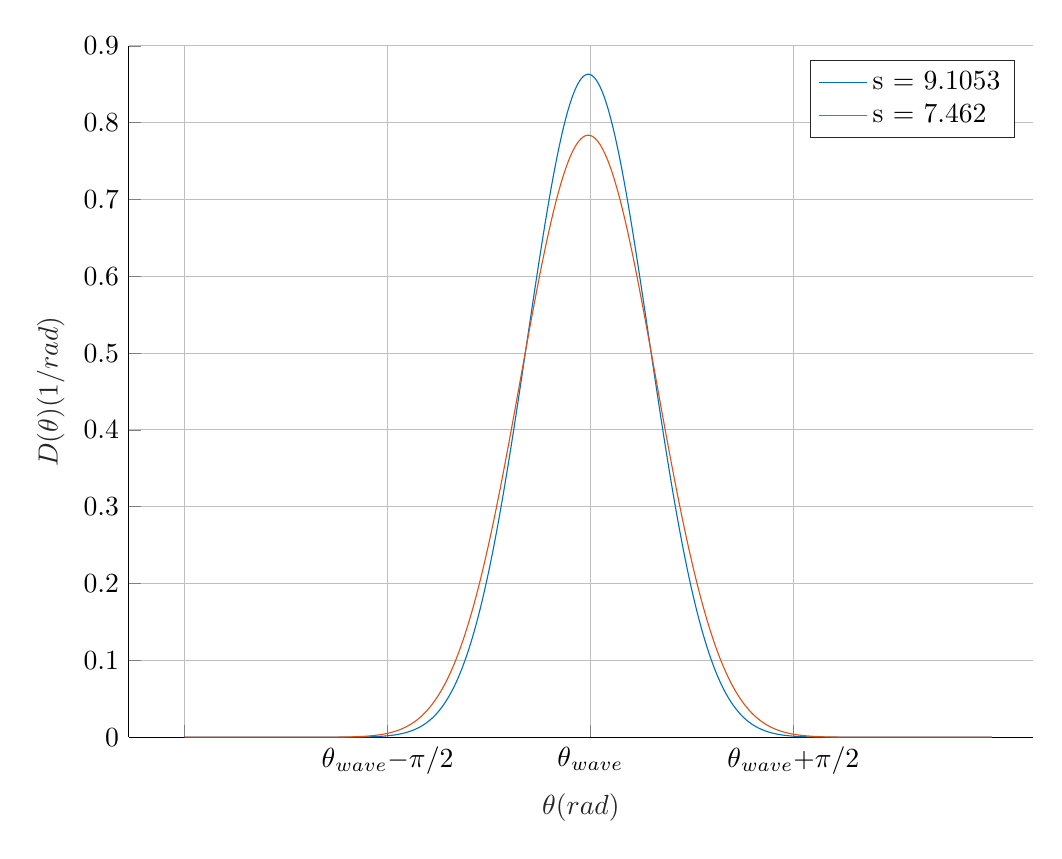
\begin{tikzpicture}

\begin{axis}[%
width=4.521in,
height=3.457in,
at={(0.758in,0.59in)},
scale only axis,
xmin=2,
xmax=9,
xtick={2.43247763855852,4.00327396535342,5.57407029214831,7.14486661894321},
xticklabels={{},{$\theta{}_{\text{wave}}\text{-}\pi\text{/2}$},{$\theta{}_{\text{wave}}$},{$\theta{}_{\text{wave}}\text{+}\pi\text{/2}$},{}},
xlabel style={font=\color{white!15!black}},
xlabel={$\theta\text{ (rad)}$},
ymin=0,
ymax=0.9,
ylabel style={font=\color{white!15!black}},
ylabel={$\text{D(}\theta\text{) (1/rad)}$},
axis background/.style={fill=white},
axis x line*=bottom,
axis y line*=left,
xmajorgrids,
ymajorgrids,
legend style={legend cell align=left, align=left, draw=white!15!black}
]
\addplot [color=mycolor1]
  table[row sep=crcr]{%
2.43247763855852	1.089904700123e-38\\
2.44470855832369	2.53928259637907e-34\\
2.45693947808885	1.59156982988422e-31\\
2.46917039785402	1.83553658139019e-29\\
2.48140131761919	7.89830854723131e-28\\
2.49363223738435	1.78097072613875e-26\\
2.50586315714952	2.54382636355025e-25\\
2.51809407691468	2.58652941526749e-24\\
2.53032499667985	2.02198059976341e-23\\
2.54255591644502	1.28197460650498e-22\\
2.55478683621018	6.85175917206531e-22\\
2.56701775597535	3.17735388940589e-21\\
2.57924867574052	1.30695963905769e-20\\
2.59147959550568	4.85180422302725e-20\\
2.60371051527085	1.64809000025001e-19\\
2.61594143503602	5.18026355870015e-19\\
2.62817235480118	1.52057306273369e-18\\
2.64040327456635	4.20017263999632e-18\\
2.65263419433151	1.09880994880626e-17\\
2.66486511409668	2.73742798874594e-17\\
2.67709603386185	6.52462467175746e-17\\
2.68932695362701	1.49386216186298e-16\\
2.70155787339218	3.29706380201836e-16\\
2.71378879315735	7.03613963297035e-16\\
2.72601971292251	1.45579369423918e-15\\
2.73825063268768	2.92722375793218e-15\\
2.75048155245284	5.73217896169244e-15\\
2.76271247221801	1.09524054371345e-14\\
2.77494339198318	2.04530626825874e-14\\
2.78717431174834	3.73874347540462e-14\\
2.79940523151351	6.69895012022819e-14\\
2.81163615127868	1.17798773683289e-13\\
2.82386707104384	2.03524962338879e-13\\
2.83609799080901	3.45846983681081e-13\\
2.84832891057418	5.78559138809039e-13\\
2.86055983033934	9.53636543450673e-13\\
2.87279075010451	1.55000403852659e-12\\
2.88502166986967	2.48607266817198e-12\\
2.89725258963484	3.93747358144406e-12\\
2.90948350940001	6.16189306796198e-12\\
2.92171442916517	9.53352117999145e-12\\
2.93394534893034	1.45904021804709e-11\\
2.94617626869551	2.20989561873611e-11\\
2.95840718846067	3.3141173155911e-11\\
2.97063810822584	4.92315159616555e-11\\
2.98286902799101	7.2472470913339e-11\\
2.99509994775617	1.05760023538176e-10\\
3.00733086752134	1.5305319791094e-10\\
3.0195617872865	2.19725274167878e-10\\
3.03179270705167	3.13018499338631e-10\\
3.04402362681684	4.42629153682584e-10\\
3.056254546582	6.21455866100742e-10\\
3.06848546634717	8.66551242044003e-10\\
3.08071638611234	1.20032534711118e-09\\
3.0929473058775	1.65205956887244e-09\\
3.10517822564267	2.25980106693913e-09\\
3.11740914540784	3.07272164500771e-09\\
3.129640065173	4.15404068650485e-09\\
3.14187098493817	5.58463005556968e-09\\
3.15410190470333	7.46743986538493e-09\\
3.1663328244685	9.93290806380005e-09\\
3.17856374423367	1.31455442080147e-08\\
3.19079466399883	1.73119089397122e-08\\
3.203025583764	2.26902458893821e-08\\
3.21525650352917	2.96020624076673e-08\\
3.22748742329433	3.84460000279712e-08\\
3.2397183430595	4.97143853023211e-08\\
3.25194926282466	6.401290702062e-08\\
3.26418018258983	8.20839272216927e-08\\
3.276411102355	1.04834001228712e-07\\
3.28864202212016	1.3336625657815e-07\\
3.30087294188533	1.6901836253135e-07\\
3.3131038616505	2.1340691121039e-07\\
3.32533478141566	2.68479128605085e-07\\
3.33756570118083	3.36572939038789e-07\\
3.349796620946	4.20486520395098e-07\\
3.36202754071116	5.23558609679019e-07\\
3.37425846047633	6.49760949435104e-07\\
3.38648938024149	8.03804405218241e-07\\
3.39872030000666	9.9126043267386e-07\\
3.41095121977183	1.21869972970344e-06\\
3.42318213953699	1.49385007443386e-06\\
3.43541305930216	1.82577552292645e-06\\
3.44764397906733	2.22507932128013e-06\\
3.45987489883249	2.70413307439155e-06\\
3.47210581859766	3.27733490738067e-06\\
3.48433673836283	3.96139955466092e-06\\
3.49656765812799	4.77568351475553e-06\\
3.50879857789316	5.74254861499264e-06\\
3.52102949765832	6.88776753772059e-06\\
3.53326041742349	8.24097506707168e-06\\
3.54549133718866	9.83616902075938e-06\\
3.55772225695382	1.17122650329346e-05\\
3.56995317671899	1.39137095495686e-05\\
3.58218409648416	1.6491155584785e-05\\
3.59441501624932	1.95022059624773e-05\\
3.60664593601449	2.30122289296466e-05\\
3.61887685577966	2.70952511732616e-05\\
3.63110777554482	3.18349333979574e-05\\
3.64333869530999	3.73256337242982e-05\\
3.65556961507515	4.36735642432158e-05\\
3.66780053484032	5.09980461080916e-05\\
3.68003145460549	5.94328685580818e-05\\
3.69226237437065	6.91277572410574e-05\\
3.70449329413582	8.02499571380708e-05\\
3.71672421390099	9.29859352798267e-05\\
3.72895513366615	0.000107543208285418\\
3.74118605343132	0.000124152299540766\\
3.75341697319648	0.000143068830565172\\
3.76564789296165	0.000164575750785491\\
3.77787881272682	0.000188985709545296\\
3.79010973249198	0.00021664357371777\\
3.80234065225715	0.000247929093762941\\
3.81457157202232	0.000283259720469646\\
3.82680249178748	0.00032309357394776\\
3.83903341155265	0.000367932565684954\\
3.85126433131782	0.000418325673652905\\
3.86349525108298	0.00047487236953937\\
3.87572617084815	0.000538226196194485\\
3.88795709061331	0.000609098492311888\\
3.90018801037848	0.000688262260218591\\
3.91241893014365	0.000776556171423222\\
3.92464984990881	0.000874888703272368\\
3.93688076967398	0.000984242398691782\\
3.94911168943915	0.00110567823954744\\
3.96134260920431	0.00124034012265378\\
3.97357352896948	0.00138945942588997\\
3.98580444873465	0.00155435965026386\\
3.99803536849981	0.00173646112209527\\
4.01026628826498	0.00193728573778349\\
4.02249720803014	0.00215846173188521\\
4.03472812779531	0.0024017284474701\\
4.04695904756048	0.00266894108595086\\
4.05918996732564	0.00296207541181323\\
4.07142088709081	0.00328323238591374\\
4.08365180685598	0.00363464269927725\\
4.09588272662114	0.00401867117763011\\
4.10811364638631	0.00443782102525945\\
4.12034456615148	0.0048947378752084\\
4.13257548591664	0.00539221361132012\\
4.14480640568181	0.00593318992623899\\
4.15703732544697	0.00652076157818838\\
4.16926824521214	0.00715817930818094\\
4.18149916497731	0.0078488523782974\\
4.19373008474247	0.00859635069081267\\
4.20596100450764	0.00940440644726175\\
4.21819192427281	0.0102769153060473\\
4.23042284403797	0.0112179369969052\\
4.24265376380314	0.0122316953504761\\
4.2548846835683	0.0133225777014083\\
4.26711560333347	0.0144951336238293\\
4.27934652309864	0.015754072958708\\
4.2915774428638	0.0171042630935826\\
4.30380836262897	0.0185507254563609\\
4.31603928239414	0.0200986311864302\\
4.3282702021593	0.0217532959481353\\
4.34050112192447	0.0235201738538139\\
4.35273204168964	0.0254048504660168\\
4.3649629614548	0.0274130348512846\\
4.37719388121997	0.0295505506609144\\
4.38942480098513	0.0318233262175123\\
4.4016557207503	0.034237383589802\\
4.41388664051547	0.0367988266421261\\
4.42611756028063	0.0395138280493386\\
4.4383484800458	0.042388615272323\\
4.45057939981097	0.0454294554941748\\
4.46281031957613	0.0486426395221425\\
4.4750412393413	0.0520344646657083\\
4.48727215910647	0.0556112166066892\\
4.49950307887163	0.059379150282928\\
4.5117339986368	0.0633444698129998\\
4.52396491840196	0.0675133074953516\\
4.53619583816713	0.071891701921398\\
4.5484267579323	0.0764855752482734\\
4.56065767769746	0.0813007096831768\\
4.57288859746263	0.0863427232374697\\
4.5851195172278	0.0916170448149217\\
4.59735043699296	0.0971288887046322\\
4.60958135675813	0.102883228555228\\
4.6218122765233	0.108884770912838\\
4.63404319628846	0.115137928411087\\
4.64627411605363	0.121646792706865\\
4.65850503581879	0.128415107260893\\
4.67073595558396	0.135446240067051\\
4.68296687534913	0.142743156439056\\
4.69519779511429	0.150308391967322\\
4.70742871487946	0.158144025762638\\
4.71965963464463	0.166251654106676\\
4.73189055440979	0.174632364632223\\
4.74412147417496	0.183286711158344\\
4.75635239394012	0.19221468930753\\
4.76858331370529	0.201415713033033\\
4.78081423347046	0.210888592185237\\
4.79304515323562	0.220631511245834\\
4.80527607300079	0.230642009357888\\
4.81750699276596	0.240916961778501\\
4.82973791253112	0.251452562878718\\
4.84196883229629	0.262244310812547\\
4.85419975206146	0.273286993973526\\
4.86643067182662	0.284574679353054\\
4.87866159159179	0.296100702909849\\
4.89089251135695	0.307857662054329\\
4.90312343112212	0.319837410345392\\
4.91535435088729	0.332031054490213\\
4.92758527065245	0.344428953730004\\
4.93981619041762	0.357020721686517\\
4.95204711018279	0.369795230735216\\
4.96427802994795	0.382740618961685\\
4.97650894971312	0.395844299747883\\
4.98873986947829	0.409092974024493\\
5.00097078924345	0.422472645214716\\
5.01320170900862	0.435968636883634\\
5.02543262877378	0.44956561309568\\
5.03766354853895	0.463247601470846\\
5.04989446830412	0.476998018918176\\
5.06212538806928	0.490799700012788\\
5.07435630783445	0.504634927970285\\
5.08658722759962	0.518485468159996\\
5.09881814736478	0.532332604086056\\
5.11104906712995	0.546157175753047\\
5.12327998689512	0.559939620320764\\
5.13551090666028	0.573660014940697\\
5.14774182642545	0.587298121655282\\
5.15997274619061	0.600833434229615\\
5.17220366595578	0.614245226774552\\
5.18443458572095	0.627512604009786\\
5.19666550548611	0.640614553005649\\
5.20889642525128	0.65352999623334\\
5.22112734501645	0.666237845744731\\
5.23335826478161	0.678717058295186\\
5.24558918454678	0.690946691215927\\
5.25782010431194	0.702905958836296\\
5.27005102407711	0.714574289251113\\
5.28228194384228	0.725931381223957\\
5.29451286360744	0.736957261013889\\
5.30674378337261	0.747632338910731\\
5.31897470313778	0.757937465262686\\
5.33120562290294	0.767853985779705\\
5.34343654266811	0.777363795896745\\
5.35566746243328	0.786449393982793\\
5.36789838219844	0.79509393318432\\
5.38012930196361	0.803281271695678\\
5.39236022172877	0.810996021253778\\
5.40459114149394	0.81822359366034\\
5.41682206125911	0.82495024514177\\
5.42905298102427	0.831163118364635\\
5.44128390078944	0.836850281933412\\
5.45351482055461	0.842000767206822\\
5.46574574031977	0.846604602279557\\
5.47797666008494	0.850652842987464\\
5.49020757985011	0.854137600806248\\
5.50243849961527	0.857052067526427\\
5.51466941938044	0.859390536600541\\
5.5269003391456	0.861148421072488\\
5.53913125891077	0.862322268013074\\
5.55136217867594	0.862909769400657\\
5.5635930984411	0.862909769400657\\
5.57582401820627	0.862322268013074\\
5.58805493797144	0.861148421072488\\
5.6002858577366	0.859390536600541\\
5.61251677750177	0.857052067526427\\
5.62474769726694	0.854137600806248\\
5.6369786170321	0.850652842987464\\
5.64920953679727	0.846604602279557\\
5.66144045656243	0.842000767206822\\
5.6736713763276	0.836850281933412\\
5.68590229609277	0.831163118364635\\
5.69813321585793	0.82495024514177\\
5.7103641356231	0.81822359366034\\
5.72259505538827	0.810996021253778\\
5.73482597515343	0.803281271695678\\
5.7470568949186	0.79509393318432\\
5.75928781468376	0.786449393982793\\
5.77151873444893	0.777363795896745\\
5.7837496542141	0.767853985779705\\
5.79598057397926	0.757937465262686\\
5.80821149374443	0.747632338910731\\
5.8204424135096	0.736957261013889\\
5.83267333327476	0.725931381223957\\
5.84490425303993	0.714574289251113\\
5.8571351728051	0.702905958836296\\
5.86936609257026	0.690946691215927\\
5.88159701233543	0.678717058295186\\
5.89382793210059	0.666237845744731\\
5.90605885186576	0.65352999623334\\
5.91828977163093	0.640614553005649\\
5.93052069139609	0.627512604009786\\
5.94275161116126	0.614245226774552\\
5.95498253092643	0.600833434229615\\
5.96721345069159	0.587298121655282\\
5.97944437045676	0.573660014940697\\
5.99167529022193	0.559939620320764\\
6.00390620998709	0.546157175753047\\
6.01613712975226	0.532332604086056\\
6.02836804951742	0.518485468159996\\
6.04059896928259	0.504634927970285\\
6.05282988904776	0.490799700012788\\
6.06506080881292	0.476998018918176\\
6.07729172857809	0.463247601470846\\
6.08952264834326	0.44956561309568\\
6.10175356810842	0.435968636883634\\
6.11398448787359	0.422472645214716\\
6.12621540763875	0.409092974024493\\
6.13844632740392	0.395844299747883\\
6.15067724716909	0.382740618961685\\
6.16290816693425	0.369795230735216\\
6.17513908669942	0.357020721686517\\
6.18737000646459	0.344428953730004\\
6.19960092622975	0.332031054490213\\
6.21183184599492	0.319837410345392\\
6.22406276576009	0.307857662054329\\
6.23629368552525	0.296100702909849\\
6.24852460529042	0.284574679353054\\
6.26075552505558	0.273286993973526\\
6.27298644482075	0.262244310812547\\
6.28521736458592	0.251452562878718\\
6.29744828435108	0.240916961778501\\
6.30967920411625	0.230642009357888\\
6.32191012388142	0.220631511245834\\
6.33414104364658	0.210888592185237\\
6.34637196341175	0.201415713033033\\
6.35860288317692	0.19221468930753\\
6.37083380294208	0.183286711158344\\
6.38306472270725	0.174632364632223\\
6.39529564247241	0.166251654106676\\
6.40752656223758	0.158144025762638\\
6.41975748200275	0.150308391967322\\
6.43198840176791	0.142743156439056\\
6.44421932153308	0.135446240067051\\
6.45645024129825	0.128415107260893\\
6.46868116106341	0.121646792706865\\
6.48091208082858	0.115137928411087\\
6.49314300059375	0.108884770912838\\
6.50537392035891	0.102883228555228\\
6.51760484012408	0.097128888704632\\
6.52983575988924	0.0916170448149217\\
6.54206667965441	0.0863427232374697\\
6.55429759941958	0.0813007096831768\\
6.56652851918474	0.0764855752482734\\
6.57875943894991	0.0718917019213976\\
6.59099035871508	0.0675133074953516\\
6.60322127848024	0.0633444698130001\\
6.61545219824541	0.059379150282928\\
6.62768311801057	0.0556112166066892\\
6.63991403777574	0.052034464665708\\
6.65214495754091	0.0486426395221425\\
6.66437587730607	0.045429455494175\\
6.67660679707124	0.042388615272323\\
6.68883771683641	0.0395138280493386\\
6.70106863660157	0.036798826642126\\
6.71329955636674	0.034237383589802\\
6.72553047613191	0.0318233262175125\\
6.73776139589707	0.0295505506609144\\
6.74999231566224	0.0274130348512846\\
6.76222323542741	0.0254048504660166\\
6.77445415519257	0.0235201738538139\\
6.78668507495774	0.0217532959481353\\
6.7989159947229	0.0200986311864302\\
6.81114691448807	0.0185507254563609\\
6.82337783425324	0.0171042630935825\\
6.8356087540184	0.015754072958708\\
6.84783967378357	0.0144951336238293\\
6.86007059354874	0.0133225777014083\\
6.8723015133139	0.0122316953504761\\
6.88453243307907	0.0112179369969052\\
6.89676335284423	0.0102769153060473\\
6.9089942726094	0.00940440644726175\\
6.92122519237457	0.00859635069081267\\
6.93345611213973	0.0078488523782974\\
6.9456870319049	0.00715817930818094\\
6.95791795167007	0.00652076157818838\\
6.97014887143523	0.00593318992623899\\
6.9823797912004	0.00539221361132012\\
6.99461071096557	0.0048947378752084\\
7.00684163073073	0.00443782102525945\\
7.0190725504959	0.00401867117763011\\
7.03130347026106	0.00363464269927725\\
7.04353439002623	0.00328323238591374\\
7.0557653097914	0.00296207541181323\\
7.06799622955656	0.00266894108595086\\
7.08022714932173	0.0024017284474701\\
7.0924580690869	0.00215846173188521\\
7.10468898885206	0.00193728573778349\\
7.11691990861723	0.00173646112209527\\
7.12915082838239	0.00155435965026386\\
7.14138174814756	0.00138945942588997\\
7.15361266791273	0.00124034012265378\\
7.16584358767789	0.00110567823954744\\
7.17807450744306	0.000984242398691782\\
7.19030542720823	0.000874888703272368\\
7.20253634697339	0.000776556171423222\\
7.21476726673856	0.000688262260218591\\
7.22699818650373	0.000609098492311891\\
7.23922910626889	0.000538226196194485\\
7.25146002603406	0.00047487236953937\\
7.26369094579923	0.000418325673652904\\
7.27592186556439	0.000367932565684954\\
7.28815278532956	0.000323093573947761\\
7.30038370509472	0.000283259720469646\\
7.31261462485989	0.000247929093762941\\
7.32484554462506	0.000216643573717768\\
7.33707646439022	0.000188985709545296\\
7.34930738415539	0.000164575750785491\\
7.36153830392056	0.000143068830565172\\
7.37376922368572	0.000124152299540766\\
7.38600014345089	0.000107543208285418\\
7.39823106321605	9.29859352798267e-05\\
7.41046198298122	8.02499571380708e-05\\
7.42269290274639	6.91277572410574e-05\\
7.43492382251155	5.94328685580818e-05\\
7.44715474227672	5.09980461080919e-05\\
7.45938566204189	4.36735642432158e-05\\
7.47161658180705	3.73256337242982e-05\\
7.48384750157222	3.18349333979574e-05\\
7.49607842133739	2.70952511732616e-05\\
7.50830934110255	2.30122289296467e-05\\
7.52054026086772	1.95022059624773e-05\\
7.53277118063288	1.6491155584785e-05\\
7.54500210039805	1.39137095495685e-05\\
7.55723302016322	1.17122650329346e-05\\
7.56946393992838	9.83616902075941e-06\\
7.58169485969355	8.24097506707168e-06\\
7.59392577945872	6.88776753772059e-06\\
7.60615669922388	5.7425486149926e-06\\
7.61838761898905	4.77568351475553e-06\\
7.63061853875421	3.96139955466092e-06\\
7.64284945851938	3.27733490738067e-06\\
7.65508037828455	2.70413307439155e-06\\
7.66731129804971	2.22507932128011e-06\\
7.67954221781488	1.82577552292645e-06\\
7.69177313758005	1.49385007443386e-06\\
7.70400405734521	1.21869972970344e-06\\
7.71623497711038	9.9126043267386e-07\\
7.72846589687555	8.03804405218248e-07\\
7.74069681664071	6.49760949435104e-07\\
7.75292773640588	5.23558609679019e-07\\
7.76515865617105	4.20486520395094e-07\\
7.77738957593621	3.36572939038789e-07\\
7.78962049570138	2.68479128605087e-07\\
7.80185141546654	2.1340691121039e-07\\
7.81408233523171	1.6901836253135e-07\\
7.82631325499688	1.33366256578149e-07\\
7.83854417476204	1.04834001228712e-07\\
7.85077509452721	8.20839272216935e-08\\
7.86300601429238	6.401290702062e-08\\
7.87523693405754	4.97143853023211e-08\\
7.88746785382271	3.84460000279708e-08\\
7.89969877358787	2.96020624076673e-08\\
7.91192969335304	2.26902458893823e-08\\
7.92416061311821	1.73119089397122e-08\\
7.93639153288337	1.31455442080147e-08\\
7.94862245264854	9.93290806379994e-09\\
7.96085337241371	7.46743986538493e-09\\
7.97308429217887	5.58463005556968e-09\\
7.98531521194404	4.15404068650485e-09\\
7.99754613170921	3.07272164500771e-09\\
8.00977705147437	2.25980106693916e-09\\
8.02200797123954	1.65205956887241e-09\\
8.0342388910047	1.20032534711116e-09\\
8.04646981076987	8.66551242043995e-10\\
8.05870073053504	6.21455866100742e-10\\
8.0709316503002	4.42629153682589e-10\\
8.08316257006537	3.13018499338639e-10\\
8.09539348983053	2.19725274167884e-10\\
8.1076244095957	1.53053197910938e-10\\
8.11985532936087	1.05760023538176e-10\\
8.13208624912603	7.24724709133401e-11\\
8.1443171688912	4.92315159616541e-11\\
8.15654808865637	3.31411731559101e-11\\
8.16877900842153	2.20989561873608e-11\\
8.1810099281867	1.45904021804709e-11\\
8.19324084795187	9.53352117999161e-12\\
8.20547176771703	6.16189306796218e-12\\
8.2177026874822	3.93747358144419e-12\\
8.22993360724737	2.48607266817194e-12\\
8.24216452701253	1.55000403852659e-12\\
8.2543954467777	9.53636543450691e-13\\
8.26662636654287	5.78559138809006e-13\\
8.27885728630803	3.45846983681068e-13\\
8.2910882060732	2.03524962338875e-13\\
8.30331912583836	1.17798773683289e-13\\
8.31555004560353	6.69895012022819e-14\\
8.3277809653687	3.7387434754047e-14\\
8.34001188513386	2.04530626825883e-14\\
8.35224280489903	1.09524054371353e-14\\
8.3644737246642	5.73217896169244e-15\\
8.37670464442936	2.92722375793218e-15\\
8.38893556419453	1.45579369423906e-15\\
8.4011664839597	7.03613963296996e-16\\
8.41339740372486	3.29706380201827e-16\\
8.42562832349003	1.49386216186298e-16\\
8.43785924325519	6.52462467175746e-17\\
8.45009016302036	2.73742798874603e-17\\
8.46232108278553	1.09880994880633e-17\\
8.47455200255069	4.20017263999677e-18\\
8.48678292231586	1.52057306273369e-18\\
8.49901384208103	5.18026355870015e-19\\
8.51124476184619	1.6480900002498e-19\\
8.52347568161136	4.8518042230268e-20\\
8.53570660137652	1.30695963905762e-20\\
8.54793752114169	3.17735388940572e-21\\
8.56016844090686	6.85175917206531e-22\\
8.57239936067202	1.28197460650506e-22\\
8.58463028043719	2.02198059976369e-23\\
8.59686120020235	2.58652941526811e-24\\
8.60909211996752	2.54382636355002e-25\\
8.62132303973269	1.78097072613875e-26\\
8.63355395949785	7.89830854723228e-28\\
8.64578487926302	1.83553658138963e-29\\
8.65801579902819	1.59156982988359e-31\\
8.67024671879335	2.53928259637836e-34\\
8.68247763855852	1.089904700123e-38\\
};
\addlegendentry{s = 9.1053}

\addplot [color=mycolor2]
  table[row sep=crcr]{%
2.43247763855852	6.84426576490762e-32\\
2.44470855832369	2.59684421254285e-28\\
2.45693947808885	5.09031053663978e-26\\
2.46917039785402	2.4920015713877e-24\\
2.48140131761919	5.43826588035286e-23\\
2.49363223738435	6.98835427276338e-22\\
2.50586315714952	6.17710002045318e-21\\
2.51809407691468	4.13268438829053e-20\\
2.53032499667985	2.22902345680389e-19\\
2.54255591644502	1.01264128317249e-18\\
2.55478683621018	3.99949011287495e-18\\
2.56701775597535	1.40612053604555e-17\\
2.57924867574052	4.48095383455307e-17\\
2.59147959550568	1.31281689597087e-16\\
2.60371051527085	3.57630246628581e-16\\
2.61594143503602	9.14199349977807e-16\\
2.62817235480118	2.2095053492284e-15\\
2.64040327456635	5.08062836848848e-15\\
2.65263419433151	1.11736601318794e-14\\
2.66486511409668	2.3608623304748e-14\\
2.67709603386185	4.8106644131395e-14\\
2.68932695362701	9.48489157915017e-14\\
2.70155787339218	1.8146713881386e-13\\
2.71378879315735	3.37746310525779e-13\\
2.72601971292251	6.12868709411088e-13\\
2.73825063268768	1.08636204918599e-12\\
2.75048155245284	1.88435858499321e-12\\
2.76271247221801	3.20335369153897e-12\\
2.77494339198318	5.34440567241069e-12\\
2.78717431174834	8.76168280267586e-12\\
2.79940523151351	1.41304848981191e-11\\
2.81163615127868	2.24413982423792e-11\\
2.82386707104384	3.51291454333504e-11\\
2.83609799080901	5.42470348910369e-11\\
2.84832891057418	8.27007764959723e-11\\
2.86055983033934	1.24558897500168e-10\\
2.87279075010451	1.85461163572134e-10\\
2.88502166986967	2.73151390714857e-10\\
2.89725258963484	3.98166942159013e-10\\
2.90948350940001	5.74724167815331e-10\\
2.92171442916517	8.21847200359553e-10\\
2.93394534893034	1.16479701946731e-09\\
2.94617626869551	1.63686869175496e-09\\
2.95840718846067	2.28163735540103e-09\\
2.97063810822584	3.15574802041381e-09\\
2.98286902799101	4.33236078072311e-09\\
2.99509994775617	5.90538177164993e-09\\
3.00733086752134	7.99463134969229e-09\\
3.0195617872865	1.07521247180757e-08\\
3.03179270705167	1.43696667696885e-08\\
3.04402362681684	1.90879924666974e-08\\
3.056254546582	2.52077168181265e-08\\
3.06848546634717	3.31023946421898e-08\\
3.08071638611234	4.32340299899673e-08\\
3.0929473058775	5.61714185304473e-08\\
3.10517822564267	7.26117535086908e-08\\
3.11740914540784	9.34059772254328e-08\\
3.129640065173	1.1958841546273e-07\\
3.14187098493817	1.52411291985674e-07\\
3.15410190470333	1.93384784244843e-07\\
3.1663328244685	2.44323349715085e-07\\
3.17856374423367	3.07399124922778e-07\\
3.19079466399883	3.85203276084701e-07\\
3.203025583764	4.8081626130983e-07\\
3.21525650352917	5.97888049354828e-07\\
3.22748742329433	7.4072942877584e-07\\
3.2397183430595	9.1441563372722e-07\\
3.25194926282466	1.12490360830653e-06\\
3.26418018258983	1.37916432985505e-06\\
3.276411102355	1.68533171254832e-06\\
3.28864202212016	2.05286971543832e-06\\
3.30087294188533	2.49275938325127e-06\\
3.3131038616505	3.01770765304587e-06\\
3.32533478141566	3.64237986456376e-06\\
3.33756570118083	4.3836580159508e-06\\
3.349796620946	5.26092690861487e-06\\
3.36202754071116	6.29639042435793e-06\\
3.37425846047633	7.51542027355113e-06\\
3.38648938024149	8.94693964391559e-06\\
3.39872030000666	1.06238442642619e-05\\
3.41095121977183	1.25834634751042e-05\\
3.42318213953699	1.48680639671076e-05\\
3.43541305930216	1.75253989075134e-05\\
3.44764397906733	2.06093052226282e-05\\
3.45987489883249	2.41803518397176e-05\\
3.47210581859766	2.83065417127732e-05\\
3.48433673836283	3.30640704621109e-05\\
3.49656765812799	3.853814444612e-05\\
3.50879857789316	4.48238610532197e-05\\
3.52102949765832	5.20271539516553e-05\\
3.53326041742349	6.02658059627537e-05\\
3.54549133718866	6.96705321281542e-05\\
3.55772225695382	8.03861354219498e-05\\
3.56995317671899	9.25727374132859e-05\\
3.58218409648416	0.000106407086012439\\
3.59441501624932	0.000122083942232593\\
3.60664593601449	0.000139817547669329\\
3.61887685577966	0.000159843174139253\\
3.63110777554482	0.0001824187566274\\
3.64333869530999	0.000207826610369319\\
3.65556961507515	0.000236375232537543\\
3.66780053484032	0.000268401188613145\\
3.68003145460549	0.000304271083100975\\
3.69226237437065	0.000344383613792176\\
3.70449329413582	0.000389171708289732\\
3.71672421390099	0.000439104740992663\\
3.72895513366615	0.000494690828182821\\
3.74118605343132	0.000556479198275778\\
3.75341697319648	0.000625062633685549\\
3.76564789296165	0.000701079980113047\\
3.77787881272682	0.000785218718402108\\
3.79010973249198	0.000878217593416764\\
3.80234065225715	0.000980869293681067\\
3.81457157202232	0.00109402317479147\\
3.82680249178748	0.0012185880188636\\
3.83903341155265	0.00135553482151384\\
3.85126433131782	0.00150589959710511\\
3.86349525108298	0.00167078619220823\\
3.87572617084815	0.00185136909645068\\
3.88795709061331	0.00204889623914627\\
3.90018801037848	0.00226469175932743\\
3.91241893014365	0.00250015873604099\\
3.92464984990881	0.00275678186502289\\
3.93688076967398	0.00303613006714268\\
3.94911168943915	0.00333985901331071\\
3.96134260920431	0.00366971354987211\\
3.97357352896948	0.00402753000788263\\
3.98580444873465	0.00441523837907145\\
3.99803536849981	0.00483486434075526\\
4.01026628826498	0.00528853111148142\\
4.02249720803014	0.00577846111874734\\
4.03472812779531	0.00630697745978007\\
4.04695904756048	0.00687650513606537\\
4.05918996732564	0.00748957204209489\\
4.07142088709081	0.00814880968866243\\
4.08365180685598	0.00885695364098502\\
4.09588272662114	0.00961684365196081\\
4.10811364638631	0.0104314234710082\\
4.12034456615148	0.0113037403091561\\
4.13257548591664	0.012236943941392\\
4.14480640568181	0.0132342854277081\\
4.15703732544697	0.0142991154348344\\
4.16926824521214	0.0154348821413079\\
4.18149916497731	0.0166451287092941\\
4.19373008474247	0.0179334903074723\\
4.20596100450764	0.0193036906702902\\
4.21819192427281	0.0207595381800227\\
4.23042284403797	0.0223049214593022\\
4.24265376380314	0.0239438044631396\\
4.2548846835683	0.0256802210609266\\
4.26711560333347	0.027518269100485\\
4.27934652309864	0.029462103947919\\
4.2915774428638	0.0315159314988248\\
4.30380836262897	0.0336840006582995\\
4.31603928239414	0.0359705952891977\\
4.3282702021593	0.0383800256301567\\
4.34050112192447	0.0409166191870887\\
4.35273204168964	0.0435847111040871\\
4.3649629614548	0.0463886340220073\\
4.37719388121997	0.0493327074353715\\
4.38942480098513	0.0524212265606736\\
4.4016557207503	0.0556584507316479\\
4.41388664051547	0.0590485913395698\\
4.42611756028063	0.0625957993392011\\
4.4383484800458	0.0663041523435348\\
4.45057939981097	0.0701776413330474\\
4.46281031957613	0.0742201570077034\\
4.4750412393413	0.0784354758124742\\
4.48727215910647	0.0828272456696125\\
4.49950307887163	0.0873989714533506\\
4.5117339986368	0.0921540002450668\\
4.52396491840196	0.0970955064092514\\
4.53619583816713	0.102226476532818\\
4.5484267579323	0.107549694272403\\
4.56065767769746	0.113067725156308\\
4.57288859746263	0.118782901389565\\
4.5851195172278	0.124697306712388\\
4.59735043699296	0.130812761363796\\
4.60958135675813	0.137130807203639\\
4.6218122765233	0.143652693047481\\
4.63404319628846	0.150379360269847\\
4.64627411605363	0.157311428732199\\
4.65850503581879	0.164449183092655\\
4.67073595558396	0.171792559554911\\
4.68296687534913	0.179341133113998\\
4.69519779511429	0.18709410535657\\
4.70742871487946	0.195050292873076\\
4.71965963464463	0.203208116338726\\
4.73189055440979	0.21156559031944\\
4.74412147417496	0.220120313857914\\
4.75635239394012	0.228869461893779\\
4.76858331370529	0.237809777570267\\
4.78081423347046	0.246937565478109\\
4.79304515323562	0.256248685885377\\
4.80527607300079	0.265738549999737\\
4.81750699276596	0.275402116307111\\
4.82973791253112	0.285233888028025\\
4.84196883229629	0.295227911729956\\
4.85419975206146	0.305377777130831\\
4.86643067182662	0.315676618125422\\
4.87866159159179	0.326117115062814\\
4.89089251135695	0.336691498299288\\
4.90312343112212	0.347391553047031\\
4.91535435088729	0.358208625534935\\
4.92758527065245	0.369133630493423\\
4.93981619041762	0.380157059970869\\
4.95204711018279	0.391268993484553\\
4.96427802994795	0.402459109504513\\
4.97650894971312	0.413716698263835\\
4.98873986947829	0.42503067588419\\
5.00097078924345	0.436389599800503\\
5.01320170900862	0.447781685463791\\
5.02543262877378	0.459194824296311\\
5.03766354853895	0.470616602868271\\
5.04989446830412	0.482034323260515\\
5.06212538806928	0.493435024572821\\
5.07435630783445	0.504805505532714\\
5.08658722759962	0.516132348155113\\
5.09881814736478	0.527401942398615\\
5.11104906712995	0.53860051175989\\
5.12327998689512	0.549714139743466\\
5.13551090666028	0.560728797140157\\
5.14774182642545	0.571630370043614\\
5.15997274619061	0.582404688530857\\
5.17220366595578	0.593037555929328\\
5.18443458572095	0.603514778589902\\
5.19666550548611	0.613822196082433\\
5.20889642525128	0.623945711727944\\
5.22112734501645	0.633871323379284\\
5.23335826478161	0.643585154360152\\
5.24558918454678	0.653073484470813\\
5.25782010431194	0.662322780967561\\
5.27005102407711	0.671319729422027\\
5.28228194384228	0.680051264365929\\
5.29451286360744	0.688504599626558\\
5.30674378337261	0.696667258258532\\
5.31897470313778	0.704527101977769\\
5.33120562290294	0.712072360004579\\
5.34343654266811	0.719291657223938\\
5.35566746243328	0.726174041572672\\
5.36789838219844	0.732709010565163\\
5.38012930196361	0.738886536871543\\
5.39236022172877	0.744697092864937\\
5.40459114149394	0.750131674057348\\
5.41682206125911	0.755181821347026\\
5.42905298102427	0.759839642003808\\
5.44128390078944	0.764097829322829\\
5.45351482055461	0.767949680881161\\
5.46574574031977	0.771389115336451\\
5.47797666008494	0.774410687711302\\
5.49020757985011	0.777009603112092\\
5.50243849961527	0.779181728836089\\
5.51466941938044	0.780923604826031\\
5.5269003391456	0.782232452436912\\
5.53913125891077	0.78310618148529\\
5.55136217867594	0.78354339555729\\
5.5635930984411	0.78354339555729\\
5.57582401820627	0.78310618148529\\
5.58805493797144	0.782232452436912\\
5.6002858577366	0.780923604826031\\
5.61251677750177	0.779181728836089\\
5.62474769726694	0.777009603112092\\
5.6369786170321	0.774410687711302\\
5.64920953679727	0.771389115336451\\
5.66144045656243	0.767949680881161\\
5.6736713763276	0.764097829322829\\
5.68590229609277	0.759839642003808\\
5.69813321585793	0.755181821347026\\
5.7103641356231	0.750131674057348\\
5.72259505538827	0.744697092864937\\
5.73482597515343	0.738886536871543\\
5.7470568949186	0.732709010565163\\
5.75928781468376	0.726174041572672\\
5.77151873444893	0.719291657223938\\
5.7837496542141	0.712072360004579\\
5.79598057397926	0.704527101977769\\
5.80821149374443	0.696667258258532\\
5.8204424135096	0.688504599626558\\
5.83267333327476	0.680051264365929\\
5.84490425303993	0.671319729422027\\
5.8571351728051	0.662322780967561\\
5.86936609257026	0.653073484470813\\
5.88159701233543	0.643585154360152\\
5.89382793210059	0.633871323379284\\
5.90605885186576	0.623945711727944\\
5.91828977163093	0.613822196082433\\
5.93052069139609	0.603514778589902\\
5.94275161116126	0.593037555929328\\
5.95498253092643	0.582404688530857\\
5.96721345069159	0.571630370043614\\
5.97944437045676	0.560728797140157\\
5.99167529022193	0.549714139743466\\
6.00390620998709	0.53860051175989\\
6.01613712975226	0.527401942398615\\
6.02836804951742	0.516132348155113\\
6.04059896928259	0.504805505532714\\
6.05282988904776	0.493435024572821\\
6.06506080881292	0.482034323260515\\
6.07729172857809	0.470616602868271\\
6.08952264834326	0.459194824296311\\
6.10175356810842	0.447781685463791\\
6.11398448787359	0.436389599800503\\
6.12621540763875	0.42503067588419\\
6.13844632740392	0.413716698263835\\
6.15067724716909	0.402459109504513\\
6.16290816693425	0.391268993484553\\
6.17513908669942	0.380157059970869\\
6.18737000646459	0.369133630493423\\
6.19960092622975	0.358208625534935\\
6.21183184599492	0.347391553047031\\
6.22406276576009	0.336691498299288\\
6.23629368552525	0.326117115062814\\
6.24852460529042	0.315676618125422\\
6.26075552505558	0.305377777130831\\
6.27298644482075	0.295227911729956\\
6.28521736458592	0.285233888028025\\
6.29744828435108	0.275402116307111\\
6.30967920411625	0.265738549999737\\
6.32191012388142	0.256248685885377\\
6.33414104364658	0.246937565478109\\
6.34637196341175	0.237809777570267\\
6.35860288317692	0.228869461893779\\
6.37083380294208	0.220120313857914\\
6.38306472270725	0.21156559031944\\
6.39529564247241	0.203208116338726\\
6.40752656223758	0.195050292873076\\
6.41975748200275	0.18709410535657\\
6.43198840176791	0.179341133113998\\
6.44421932153308	0.171792559554911\\
6.45645024129825	0.164449183092655\\
6.46868116106341	0.157311428732199\\
6.48091208082858	0.150379360269847\\
6.49314300059375	0.143652693047481\\
6.50537392035891	0.137130807203639\\
6.51760484012408	0.130812761363795\\
6.52983575988924	0.124697306712388\\
6.54206667965441	0.118782901389565\\
6.55429759941958	0.113067725156308\\
6.56652851918474	0.107549694272403\\
6.57875943894991	0.102226476532817\\
6.59099035871508	0.0970955064092514\\
6.60322127848024	0.0921540002450671\\
6.61545219824541	0.0873989714533506\\
6.62768311801057	0.0828272456696125\\
6.63991403777574	0.0784354758124739\\
6.65214495754091	0.0742201570077034\\
6.66437587730607	0.0701776413330477\\
6.67660679707124	0.0663041523435348\\
6.68883771683641	0.0625957993392011\\
6.70106863660157	0.0590485913395696\\
6.71329955636674	0.0556584507316479\\
6.72553047613191	0.0524212265606738\\
6.73776139589707	0.0493327074353715\\
6.74999231566224	0.0463886340220073\\
6.76222323542741	0.0435847111040868\\
6.77445415519257	0.0409166191870887\\
6.78668507495774	0.0383800256301567\\
6.7989159947229	0.0359705952891977\\
6.81114691448807	0.0336840006582995\\
6.82337783425324	0.0315159314988246\\
6.8356087540184	0.029462103947919\\
6.84783967378357	0.027518269100485\\
6.86007059354874	0.0256802210609266\\
6.8723015133139	0.0239438044631396\\
6.88453243307907	0.0223049214593022\\
6.89676335284423	0.0207595381800227\\
6.9089942726094	0.0193036906702902\\
6.92122519237457	0.0179334903074723\\
6.93345611213973	0.0166451287092941\\
6.9456870319049	0.0154348821413079\\
6.95791795167007	0.0142991154348344\\
6.97014887143523	0.0132342854277081\\
6.9823797912004	0.012236943941392\\
6.99461071096557	0.0113037403091561\\
7.00684163073073	0.0104314234710082\\
7.0190725504959	0.00961684365196081\\
7.03130347026106	0.00885695364098502\\
7.04353439002623	0.00814880968866243\\
7.0557653097914	0.00748957204209489\\
7.06799622955656	0.00687650513606537\\
7.08022714932173	0.00630697745978007\\
7.0924580690869	0.00577846111874734\\
7.10468898885206	0.00528853111148142\\
7.11691990861723	0.00483486434075526\\
7.12915082838239	0.00441523837907145\\
7.14138174814756	0.00402753000788263\\
7.15361266791273	0.00366971354987211\\
7.16584358767789	0.00333985901331072\\
7.17807450744306	0.00303613006714268\\
7.19030542720823	0.00275678186502289\\
7.20253634697339	0.00250015873604099\\
7.21476726673856	0.00226469175932743\\
7.22699818650373	0.00204889623914628\\
7.23922910626889	0.00185136909645068\\
7.25146002603406	0.00167078619220823\\
7.26369094579923	0.0015058995971051\\
7.27592186556439	0.00135553482151384\\
7.28815278532956	0.0012185880188636\\
7.30038370509472	0.00109402317479147\\
7.31261462485989	0.000980869293681067\\
7.32484554462506	0.00087821759341676\\
7.33707646439022	0.000785218718402108\\
7.34930738415539	0.000701079980113047\\
7.36153830392056	0.000625062633685549\\
7.37376922368572	0.000556479198275778\\
7.38600014345089	0.000494690828182819\\
7.39823106321605	0.000439104740992663\\
7.41046198298122	0.000389171708289732\\
7.42269290274639	0.000344383613792176\\
7.43492382251155	0.000304271083100975\\
7.44715474227672	0.000268401188613147\\
7.45938566204189	0.000236375232537543\\
7.47161658180705	0.000207826610369319\\
7.48384750157222	0.0001824187566274\\
7.49607842133739	0.000159843174139253\\
7.50830934110255	0.000139817547669329\\
7.52054026086772	0.000122083942232593\\
7.53277118063288	0.000106407086012439\\
7.54500210039805	9.25727374132854e-05\\
7.55723302016322	8.03861354219498e-05\\
7.56946393992838	6.96705321281544e-05\\
7.58169485969355	6.02658059627537e-05\\
7.59392577945872	5.20271539516553e-05\\
7.60615669922388	4.48238610532194e-05\\
7.61838761898905	3.853814444612e-05\\
7.63061853875421	3.30640704621109e-05\\
7.64284945851938	2.83065417127732e-05\\
7.65508037828455	2.41803518397176e-05\\
7.66731129804971	2.06093052226281e-05\\
7.67954221781488	1.75253989075134e-05\\
7.69177313758005	1.48680639671076e-05\\
7.70400405734521	1.25834634751042e-05\\
7.71623497711038	1.06238442642619e-05\\
7.72846589687555	8.94693964391566e-06\\
7.74069681664071	7.51542027355113e-06\\
7.75292773640588	6.29639042435793e-06\\
7.76515865617105	5.26092690861483e-06\\
7.77738957593621	4.3836580159508e-06\\
7.78962049570138	3.64237986456379e-06\\
7.80185141546654	3.01770765304587e-06\\
7.81408233523171	2.49275938325127e-06\\
7.82631325499688	2.05286971543831e-06\\
7.83854417476204	1.68533171254832e-06\\
7.85077509452721	1.37916432985506e-06\\
7.86300601429238	1.12490360830653e-06\\
7.87523693405754	9.1441563372722e-07\\
7.88746785382271	7.40729428775834e-07\\
7.89969877358787	5.97888049354828e-07\\
7.91192969335304	4.80816261309833e-07\\
7.92416061311821	3.85203276084701e-07\\
7.93639153288337	3.07399124922778e-07\\
7.94862245264854	2.44323349715083e-07\\
7.96085337241371	1.93384784244843e-07\\
7.97308429217887	1.52411291985674e-07\\
7.98531521194404	1.1958841546273e-07\\
7.99754613170921	9.34059772254328e-08\\
8.00977705147437	7.26117535086915e-08\\
8.02200797123954	5.61714185304463e-08\\
8.0342388910047	4.32340299899665e-08\\
8.04646981076987	3.31023946421896e-08\\
8.05870073053504	2.52077168181265e-08\\
8.0709316503002	1.90879924666976e-08\\
8.08316257006537	1.43696667696888e-08\\
8.09539348983053	1.07521247180759e-08\\
8.1076244095957	7.9946313496922e-09\\
8.11985532936087	5.90538177164993e-09\\
8.13208624912603	4.33236078072316e-09\\
8.1443171688912	3.15574802041373e-09\\
8.15654808865637	2.28163735540098e-09\\
8.16877900842153	1.63686869175494e-09\\
8.1810099281867	1.16479701946731e-09\\
8.19324084795187	8.21847200359564e-10\\
8.20547176771703	5.74724167815347e-10\\
8.2177026874822	3.98166942159023e-10\\
8.22993360724737	2.73151390714853e-10\\
8.24216452701253	1.85461163572134e-10\\
8.2543954467777	1.2455889750017e-10\\
8.26662636654287	8.27007764959685e-11\\
8.27885728630803	5.42470348910351e-11\\
8.2910882060732	3.51291454333498e-11\\
8.30331912583836	2.24413982423792e-11\\
8.31555004560353	1.41304848981191e-11\\
8.3277809653687	8.76168280267602e-12\\
8.34001188513386	5.34440567241089e-12\\
8.35224280489903	3.20335369153915e-12\\
8.3644737246642	1.88435858499321e-12\\
8.37670464442936	1.08636204918599e-12\\
8.38893556419453	6.12868709411049e-13\\
8.4011664839597	3.37746310525764e-13\\
8.41339740372486	1.81467138813855e-13\\
8.42562832349003	9.48489157915017e-14\\
8.43785924325519	4.8106644131395e-14\\
8.45009016302036	2.36086233047487e-14\\
8.46232108278553	1.11736601318801e-14\\
8.47455200255069	5.08062836848893e-15\\
8.48678292231586	2.2095053492284e-15\\
8.49901384208103	9.14199349977807e-16\\
8.51124476184619	3.57630246628543e-16\\
8.52347568161136	1.31281689597077e-16\\
8.53570660137652	4.48095383455288e-17\\
8.54793752114169	1.40612053604549e-17\\
8.56016844090686	3.99949011287495e-18\\
8.57239936067202	1.01264128317255e-18\\
8.58463028043719	2.22902345680415e-19\\
8.59686120020235	4.13268438829133e-20\\
8.60909211996752	6.17710002045272e-21\\
8.62132303973269	6.98835427276338e-22\\
8.63355395949785	5.43826588035341e-23\\
8.64578487926302	2.49200157138708e-24\\
8.65801579902819	5.09031053663813e-26\\
8.67024671879335	2.59684421254226e-28\\
8.68247763855852	6.84426576490762e-32\\
};
\addlegendentry{s = 7.462}

\end{axis}
\end{tikzpicture}%}
    \caption{Directional distribution function, $D(\theta)$, defined using the $\cos^2(\theta)$ model detailed in Section \ref{subsec:theory.waves.modelling}.}
    \label{fig:systemDesign.direcDistributionFunction}
\end{figure}

% Generate 2D spectrum from 1D eq
In accordance with Equation xx, the two-dimensional directional wave spectrum can be obtained by multiplying the one-dimensional wave spectrum, $E(\omega)$, with the directional distribution function, $D(\theta)$. This was achieved using the \href{https://github.com/JNSRYA006/sar-parameter-extraction-pipeline/blob/main/functions/waveSpectra/generate2DWaveSpectrum.m}{\lstinline{generate2DWaveSpectrum}} block, which took in the one-dimensional wave spectrum, and the directional distribution function and simply performed an element-wise multiplication using \textsc{Matlab}'s built-in 'dot' multiplication. This resulted in the two-dimensional wave spectrum shown in Figure \ref{fig:systemDesign.2DSampleWaveSpectrum}
% INCREASE SURF FONT SIZE
\begin{figure} [H]
    \centering
    \subcaptionbox{Contour plot of the two-dimensional wave spectrum, E($\omega,\theta$). \label{fig:systemDesign.2DSampleWaveSpectrumContour}}[0.48\linewidth]{
        \resizebox{\linewidth}{!}{% This file was created by matlab2tikz.
%
%The latest updates can be retrieved from
%  http://www.mathworks.com/matlabcentral/fileexchange/22022-matlab2tikz-matlab2tikz
%where you can also make suggestions and rate matlab2tikz.
%
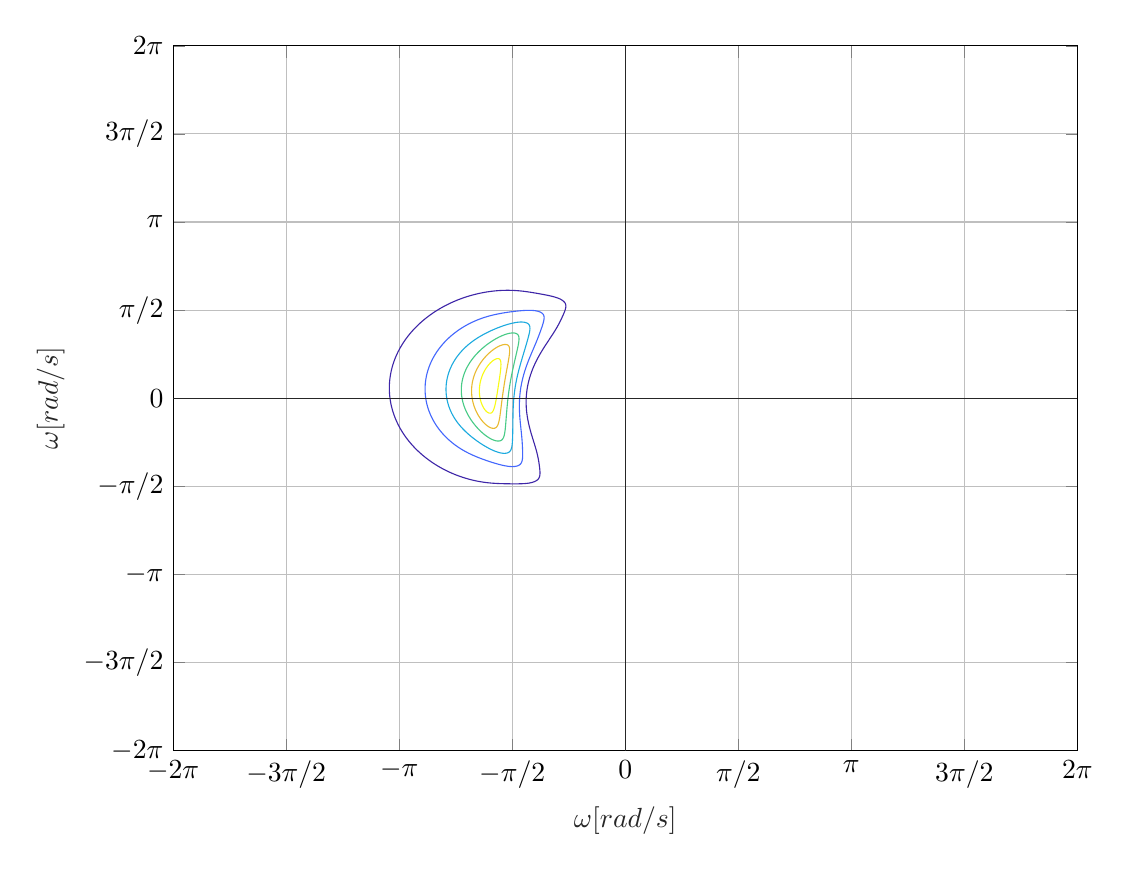
\begin{tikzpicture}

\begin{axis}[%
width=4.521in,
height=3.524in,
at={(0.758in,0.523in)},
scale only axis,
colormap={mymap}{[1pt] rgb(0pt)=(0.2422,0.1504,0.6603); rgb(1pt)=(0.2444,0.1534,0.6728); rgb(2pt)=(0.2464,0.1569,0.6847); rgb(3pt)=(0.2484,0.1607,0.6961); rgb(4pt)=(0.2503,0.1648,0.7071); rgb(5pt)=(0.2522,0.1689,0.7179); rgb(6pt)=(0.254,0.1732,0.7286); rgb(7pt)=(0.2558,0.1773,0.7393); rgb(8pt)=(0.2576,0.1814,0.7501); rgb(9pt)=(0.2594,0.1854,0.761); rgb(11pt)=(0.2628,0.1932,0.7828); rgb(12pt)=(0.2645,0.1972,0.7937); rgb(13pt)=(0.2661,0.2011,0.8043); rgb(14pt)=(0.2676,0.2052,0.8148); rgb(15pt)=(0.2691,0.2094,0.8249); rgb(16pt)=(0.2704,0.2138,0.8346); rgb(17pt)=(0.2717,0.2184,0.8439); rgb(18pt)=(0.2729,0.2231,0.8528); rgb(19pt)=(0.274,0.228,0.8612); rgb(20pt)=(0.2749,0.233,0.8692); rgb(21pt)=(0.2758,0.2382,0.8767); rgb(22pt)=(0.2766,0.2435,0.884); rgb(23pt)=(0.2774,0.2489,0.8908); rgb(24pt)=(0.2781,0.2543,0.8973); rgb(25pt)=(0.2788,0.2598,0.9035); rgb(26pt)=(0.2794,0.2653,0.9094); rgb(27pt)=(0.2798,0.2708,0.915); rgb(28pt)=(0.2802,0.2764,0.9204); rgb(29pt)=(0.2806,0.2819,0.9255); rgb(30pt)=(0.2809,0.2875,0.9305); rgb(31pt)=(0.2811,0.293,0.9352); rgb(32pt)=(0.2813,0.2985,0.9397); rgb(33pt)=(0.2814,0.304,0.9441); rgb(34pt)=(0.2814,0.3095,0.9483); rgb(35pt)=(0.2813,0.315,0.9524); rgb(36pt)=(0.2811,0.3204,0.9563); rgb(37pt)=(0.2809,0.3259,0.96); rgb(38pt)=(0.2807,0.3313,0.9636); rgb(39pt)=(0.2803,0.3367,0.967); rgb(40pt)=(0.2798,0.3421,0.9702); rgb(41pt)=(0.2791,0.3475,0.9733); rgb(42pt)=(0.2784,0.3529,0.9763); rgb(43pt)=(0.2776,0.3583,0.9791); rgb(44pt)=(0.2766,0.3638,0.9817); rgb(45pt)=(0.2754,0.3693,0.984); rgb(46pt)=(0.2741,0.3748,0.9862); rgb(47pt)=(0.2726,0.3804,0.9881); rgb(48pt)=(0.271,0.386,0.9898); rgb(49pt)=(0.2691,0.3916,0.9912); rgb(50pt)=(0.267,0.3973,0.9924); rgb(51pt)=(0.2647,0.403,0.9935); rgb(52pt)=(0.2621,0.4088,0.9946); rgb(53pt)=(0.2591,0.4145,0.9955); rgb(54pt)=(0.2556,0.4203,0.9965); rgb(55pt)=(0.2517,0.4261,0.9974); rgb(56pt)=(0.2473,0.4319,0.9983); rgb(57pt)=(0.2424,0.4378,0.9991); rgb(58pt)=(0.2369,0.4437,0.9996); rgb(59pt)=(0.2311,0.4497,0.9995); rgb(60pt)=(0.225,0.4559,0.9985); rgb(61pt)=(0.2189,0.462,0.9968); rgb(62pt)=(0.2128,0.4682,0.9948); rgb(63pt)=(0.2066,0.4743,0.9926); rgb(64pt)=(0.2006,0.4803,0.9906); rgb(65pt)=(0.195,0.4861,0.9887); rgb(66pt)=(0.1903,0.4919,0.9867); rgb(67pt)=(0.1869,0.4975,0.9844); rgb(68pt)=(0.1847,0.503,0.9819); rgb(69pt)=(0.1831,0.5084,0.9793); rgb(70pt)=(0.1818,0.5138,0.9766); rgb(71pt)=(0.1806,0.5191,0.9738); rgb(72pt)=(0.1795,0.5244,0.9709); rgb(73pt)=(0.1785,0.5296,0.9677); rgb(74pt)=(0.1778,0.5349,0.9641); rgb(75pt)=(0.1773,0.5401,0.9602); rgb(76pt)=(0.1768,0.5452,0.956); rgb(77pt)=(0.1764,0.5504,0.9516); rgb(78pt)=(0.1755,0.5554,0.9473); rgb(79pt)=(0.174,0.5605,0.9432); rgb(80pt)=(0.1716,0.5655,0.9393); rgb(81pt)=(0.1686,0.5705,0.9357); rgb(82pt)=(0.1649,0.5755,0.9323); rgb(83pt)=(0.161,0.5805,0.9289); rgb(84pt)=(0.1573,0.5854,0.9254); rgb(85pt)=(0.154,0.5902,0.9218); rgb(86pt)=(0.1513,0.595,0.9182); rgb(87pt)=(0.1492,0.5997,0.9147); rgb(88pt)=(0.1475,0.6043,0.9113); rgb(89pt)=(0.1461,0.6089,0.908); rgb(90pt)=(0.1446,0.6135,0.905); rgb(91pt)=(0.1429,0.618,0.9022); rgb(92pt)=(0.1408,0.6226,0.8998); rgb(93pt)=(0.1383,0.6272,0.8975); rgb(94pt)=(0.1354,0.6317,0.8953); rgb(95pt)=(0.1321,0.6363,0.8932); rgb(96pt)=(0.1288,0.6408,0.891); rgb(97pt)=(0.1253,0.6453,0.8887); rgb(98pt)=(0.1219,0.6497,0.8862); rgb(99pt)=(0.1185,0.6541,0.8834); rgb(100pt)=(0.1152,0.6584,0.8804); rgb(101pt)=(0.1119,0.6627,0.877); rgb(102pt)=(0.1085,0.6669,0.8734); rgb(103pt)=(0.1048,0.671,0.8695); rgb(104pt)=(0.1009,0.675,0.8653); rgb(105pt)=(0.0964,0.6789,0.8609); rgb(106pt)=(0.0914,0.6828,0.8562); rgb(107pt)=(0.0855,0.6865,0.8513); rgb(108pt)=(0.0789,0.6902,0.8462); rgb(109pt)=(0.0713,0.6938,0.8409); rgb(110pt)=(0.0628,0.6972,0.8355); rgb(111pt)=(0.0535,0.7006,0.8299); rgb(112pt)=(0.0433,0.7039,0.8242); rgb(113pt)=(0.0328,0.7071,0.8183); rgb(114pt)=(0.0234,0.7103,0.8124); rgb(115pt)=(0.0155,0.7133,0.8064); rgb(116pt)=(0.0091,0.7163,0.8003); rgb(117pt)=(0.0046,0.7192,0.7941); rgb(118pt)=(0.0019,0.722,0.7878); rgb(119pt)=(0.0009,0.7248,0.7815); rgb(120pt)=(0.0018,0.7275,0.7752); rgb(121pt)=(0.0046,0.7301,0.7688); rgb(122pt)=(0.0094,0.7327,0.7623); rgb(123pt)=(0.0162,0.7352,0.7558); rgb(124pt)=(0.0253,0.7376,0.7492); rgb(125pt)=(0.0369,0.74,0.7426); rgb(126pt)=(0.0504,0.7423,0.7359); rgb(127pt)=(0.0638,0.7446,0.7292); rgb(128pt)=(0.077,0.7468,0.7224); rgb(129pt)=(0.0899,0.7489,0.7156); rgb(130pt)=(0.1023,0.751,0.7088); rgb(131pt)=(0.1141,0.7531,0.7019); rgb(132pt)=(0.1252,0.7552,0.695); rgb(133pt)=(0.1354,0.7572,0.6881); rgb(134pt)=(0.1448,0.7593,0.6812); rgb(135pt)=(0.1532,0.7614,0.6741); rgb(136pt)=(0.1609,0.7635,0.6671); rgb(137pt)=(0.1678,0.7656,0.6599); rgb(138pt)=(0.1741,0.7678,0.6527); rgb(139pt)=(0.1799,0.7699,0.6454); rgb(140pt)=(0.1853,0.7721,0.6379); rgb(141pt)=(0.1905,0.7743,0.6303); rgb(142pt)=(0.1954,0.7765,0.6225); rgb(143pt)=(0.2003,0.7787,0.6146); rgb(144pt)=(0.2061,0.7808,0.6065); rgb(145pt)=(0.2118,0.7828,0.5983); rgb(146pt)=(0.2178,0.7849,0.5899); rgb(147pt)=(0.2244,0.7869,0.5813); rgb(148pt)=(0.2318,0.7887,0.5725); rgb(149pt)=(0.2401,0.7905,0.5636); rgb(150pt)=(0.2491,0.7922,0.5546); rgb(151pt)=(0.2589,0.7937,0.5454); rgb(152pt)=(0.2695,0.7951,0.536); rgb(153pt)=(0.2809,0.7964,0.5266); rgb(154pt)=(0.2929,0.7975,0.517); rgb(155pt)=(0.3052,0.7985,0.5074); rgb(156pt)=(0.3176,0.7994,0.4975); rgb(157pt)=(0.3301,0.8002,0.4876); rgb(158pt)=(0.3424,0.8009,0.4774); rgb(159pt)=(0.3548,0.8016,0.4669); rgb(160pt)=(0.3671,0.8021,0.4563); rgb(161pt)=(0.3795,0.8026,0.4454); rgb(162pt)=(0.3921,0.8029,0.4344); rgb(163pt)=(0.405,0.8031,0.4233); rgb(164pt)=(0.4184,0.803,0.4122); rgb(165pt)=(0.4322,0.8028,0.4013); rgb(166pt)=(0.4463,0.8024,0.3904); rgb(167pt)=(0.4608,0.8018,0.3797); rgb(168pt)=(0.4753,0.8011,0.3691); rgb(169pt)=(0.4899,0.8002,0.3586); rgb(170pt)=(0.5044,0.7993,0.348); rgb(171pt)=(0.5187,0.7982,0.3374); rgb(172pt)=(0.5329,0.797,0.3267); rgb(173pt)=(0.547,0.7957,0.3159); rgb(175pt)=(0.5748,0.7929,0.2941); rgb(176pt)=(0.5886,0.7913,0.2833); rgb(177pt)=(0.6024,0.7896,0.2726); rgb(178pt)=(0.6161,0.7878,0.2622); rgb(179pt)=(0.6297,0.7859,0.2521); rgb(180pt)=(0.6433,0.7839,0.2423); rgb(181pt)=(0.6567,0.7818,0.2329); rgb(182pt)=(0.6701,0.7796,0.2239); rgb(183pt)=(0.6833,0.7773,0.2155); rgb(184pt)=(0.6963,0.775,0.2075); rgb(185pt)=(0.7091,0.7727,0.1998); rgb(186pt)=(0.7218,0.7703,0.1924); rgb(187pt)=(0.7344,0.7679,0.1852); rgb(188pt)=(0.7468,0.7654,0.1782); rgb(189pt)=(0.759,0.7629,0.1717); rgb(190pt)=(0.771,0.7604,0.1658); rgb(191pt)=(0.7829,0.7579,0.1608); rgb(192pt)=(0.7945,0.7554,0.157); rgb(193pt)=(0.806,0.7529,0.1546); rgb(194pt)=(0.8172,0.7505,0.1535); rgb(195pt)=(0.8281,0.7481,0.1536); rgb(196pt)=(0.8389,0.7457,0.1546); rgb(197pt)=(0.8495,0.7435,0.1564); rgb(198pt)=(0.86,0.7413,0.1587); rgb(199pt)=(0.8703,0.7392,0.1615); rgb(200pt)=(0.8804,0.7372,0.165); rgb(201pt)=(0.8903,0.7353,0.1695); rgb(202pt)=(0.9,0.7336,0.1749); rgb(203pt)=(0.9093,0.7321,0.1815); rgb(204pt)=(0.9184,0.7308,0.189); rgb(205pt)=(0.9272,0.7298,0.1973); rgb(206pt)=(0.9357,0.729,0.2061); rgb(207pt)=(0.944,0.7285,0.2151); rgb(208pt)=(0.9523,0.7284,0.2237); rgb(209pt)=(0.9606,0.7285,0.2312); rgb(210pt)=(0.9689,0.7292,0.2373); rgb(211pt)=(0.977,0.7304,0.2418); rgb(212pt)=(0.9842,0.733,0.2446); rgb(213pt)=(0.99,0.7365,0.2429); rgb(214pt)=(0.9946,0.7407,0.2394); rgb(215pt)=(0.9966,0.7458,0.2351); rgb(216pt)=(0.9971,0.7513,0.2309); rgb(217pt)=(0.9972,0.7569,0.2267); rgb(218pt)=(0.9971,0.7626,0.2224); rgb(219pt)=(0.9969,0.7683,0.2181); rgb(220pt)=(0.9966,0.774,0.2138); rgb(221pt)=(0.9962,0.7798,0.2095); rgb(222pt)=(0.9957,0.7856,0.2053); rgb(223pt)=(0.9949,0.7915,0.2012); rgb(224pt)=(0.9938,0.7974,0.1974); rgb(225pt)=(0.9923,0.8034,0.1939); rgb(226pt)=(0.9906,0.8095,0.1906); rgb(227pt)=(0.9885,0.8156,0.1875); rgb(228pt)=(0.9861,0.8218,0.1846); rgb(229pt)=(0.9835,0.828,0.1817); rgb(230pt)=(0.9807,0.8342,0.1787); rgb(231pt)=(0.9778,0.8404,0.1757); rgb(232pt)=(0.9748,0.8467,0.1726); rgb(233pt)=(0.972,0.8529,0.1695); rgb(234pt)=(0.9694,0.8591,0.1665); rgb(235pt)=(0.9671,0.8654,0.1636); rgb(236pt)=(0.9651,0.8716,0.1608); rgb(237pt)=(0.9634,0.8778,0.1582); rgb(238pt)=(0.9619,0.884,0.1557); rgb(239pt)=(0.9608,0.8902,0.1532); rgb(240pt)=(0.9601,0.8963,0.1507); rgb(241pt)=(0.9596,0.9023,0.148); rgb(242pt)=(0.9595,0.9084,0.145); rgb(243pt)=(0.9597,0.9143,0.1418); rgb(244pt)=(0.9601,0.9203,0.1382); rgb(245pt)=(0.9608,0.9262,0.1344); rgb(246pt)=(0.9618,0.932,0.1304); rgb(247pt)=(0.9629,0.9379,0.1261); rgb(248pt)=(0.9642,0.9437,0.1216); rgb(249pt)=(0.9657,0.9494,0.1168); rgb(250pt)=(0.9674,0.9552,0.1116); rgb(251pt)=(0.9692,0.9609,0.1061); rgb(252pt)=(0.9711,0.9667,0.1001); rgb(253pt)=(0.973,0.9724,0.0938); rgb(254pt)=(0.9749,0.9782,0.0872); rgb(255pt)=(0.9769,0.9839,0.0805)},
xmin=-6.28314603007756,
xmax=6.28309740651393,
xtick={-6.28318530717959,-4.71238898038469,-3.14159265358979,-1.5707963267949,0,1.5707963267949,3.14159265358979,4.71238898038469,6.28318530717959},
xticklabels={{$\text{-2}\pi$},{$\text{-3}\pi\text{/2}$},{$\text{-}\pi$},{$\text{-}\pi\text{/2}$},{0},{$\pi\text{/2}$},{$\pi$},{$\text{3}\pi\text{/2}$},{$\text{2}\pi$}},
xlabel style={font=\color{white!15!black}},
xlabel={$\omega\text{ [rad/s]}$},
ymin=-6.28314777417338,
ymax=6.28317619871742,
ytick={-6.28318530717959,-4.71238898038469,-3.14159265358979,-1.5707963267949,0,1.5707963267949,3.14159265358979,4.71238898038469,6.28318530717959},
yticklabels={{$\text{-2}\pi$},{$\text{-3}\pi\text{/2}$},{$\text{-}\pi$},{$\text{-}\pi\text{/2}$},{0},{$\pi\text{/2}$},{$\pi$},{$\text{3}\pi\text{/2}$},{$\text{2}\pi$}},
ylabel style={font=\color{white!15!black}},
ylabel={$\omega\text{ [rad/s]}$},
axis background/.style={fill=white},
xmajorgrids,
ymajorgrids
]
\addplot[contour prepared, contour prepared format=matlab, contour/labels=false] table[row sep=crcr] {%
%
0.002	637\\
-1.33380377033487	0.3426608092345\\
-1.33477352645652	0.338200589309501\\
-1.33821270585278	0.321706580662239\\
-1.34151107603817	0.305193367398389\\
-1.34466788562761	0.288660947488467\\
-1.34768246180424	0.272109379090275\\
-1.35055421027367	0.255538774140962\\
-1.35328261530342	0.238949292124529\\
-1.35586723984878	0.222341133991142\\
-1.35830772576624	0.205714536205415\\
-1.36060379411608	0.18906976490145\\
-1.36275524555571	0.17240711012297\\
-1.36476196082554	0.155726880127302\\
-1.36662390132959	0.139029395732243\\
-1.36834110981288	0.122314984685085\\
-1.36991371113828	0.105583976033093\\
-1.37134191316538	0.0888366944747663\\
-1.37262600773451	0.0720734546710337\\
-1.37376637175912	0.0552945554953065\\
-1.37476346842998	0.0385002742009574\\
-1.37561784853516	0.021690860484297\\
-1.37633015189993	0.00486653042055352\\
-1.37690110895096	-0.0119725397503763\\
-1.37701688633944	-0.0165354975971162\\
-1.37730438439104	-0.0288256516213368\\
-1.37755439620993	-0.0456921785641399\\
-1.37766213312904	-0.0625720533921455\\
-1.37762865092655	-0.0794651848268223\\
-1.37745510204036	-0.0963715516561133\\
-1.3771427378601	-0.113291209996354\\
-1.37669291117647	-0.130224300879789\\
-1.37610707879531	-0.147171058199978\\
-1.37538680432427	-0.164131817049468\\
-1.37453376114066	-0.181107022486328\\
-1.37354973554934	-0.198097238768676\\
-1.37243663014026	-0.215103159099019\\
-1.37223465170278	-0.217842457089767\\
-1.37113567837666	-0.232115325144674\\
-1.3696943941691	-0.249140672368272\\
-1.36812650862225	-0.26618197804765\\
-1.36643433368436	-0.283240375632039\\
-1.36462031262093	-0.300317176807098\\
-1.36268702457165	-0.317413884712501\\
-1.36063718937859	-0.334532208020238\\
-1.36003651473398	-0.339240471753706\\
-1.35841092075788	-0.35165783107304\\
-1.35604658676595	-0.368800069228188\\
-1.3535707358613	-0.385966907258457\\
-1.35098659250334	-0.403160817481237\\
-1.34829754469627	-0.420384551766442\\
-1.34642532221971	-0.431898863951165\\
-1.34547680799732	-0.437631292403529\\
-1.34249461461347	-0.454891823894516\\
-1.33941480809917	-0.472188355688433\\
-1.33624137945805	-0.489524733794813\\
-1.33297851346562	-0.506905185809981\\
-1.33274690943558	-0.508089508189898\\
-1.32954417913089	-0.5243002700032\\
-1.32601947913864	-0.541742636052628\\
-1.32241532007497	-0.559239941788599\\
-1.31948253231791	-0.573176013798169\\
-1.3187186646266	-0.576790118861399\\
-1.31488120235764	-0.594374521929754\\
-1.31097628223918	-0.612028567300472\\
-1.30700943802328	-0.629759477833273\\
-1.30691519893558	-0.630166867370654\\
-1.302907117067	-0.647535675870102\\
-1.29874980496557	-0.665400174984221\\
-1.29510611019128	-0.680910323954787\\
-1.29453602270667	-0.683357837314606\\
-1.29021979984248	-0.701389462717174\\
-1.2858673315338	-0.719535912096496\\
-1.28412177178062	-0.726680042840624\\
-1.281449891487	-0.737787861867805\\
-1.2769858648245	-0.756162287346283\\
-1.27399636864361	-0.768378639100403\\
-1.2724901379804	-0.774675522109746\\
-1.26795511045561	-0.793331145256728\\
-1.26470125917161	-0.806688892706619\\
-1.26340942580894	-0.812155866348007\\
-1.25884798653392	-0.83115647807244\\
-1.25619997998464	-0.842142776807644\\
-1.25429436563514	-0.850359287306295\\
-1.2497551764179	-0.869780953839724\\
-1.24848093149283	-0.875154797117137\\
-1.2452475217892	-0.889446648227521\\
-1.2414920521638	-0.906071088823026\\
-1.24078469268454	-0.909380605879737\\
-1.23638466522186	-0.929612252892127\\
-1.23515760587245	-0.93518892329315\\
-1.23206539958765	-0.950173126744342\\
-1.22945486196052	-0.962739960857996\\
-1.22784100220404	-0.971093958108584\\
-1.22435830043796	-0.988920773676599\\
-1.22372941721472	-0.992410650456685\\
-1.21978903868883	-1.01391997081081\\
-1.21974852475607	-1.01416155351782\\
-1.21591486045942	-1.03638651677274\\
-1.2156451028612	-1.03791302685229\\
-1.21223557383554	-1.05911988489227\\
-1.21192123545224	-1.06101757987397\\
-1.2087163531784	-1.08239674465521\\
-1.20856772472476	-1.08335222935586\\
-1.20551057776999	-1.10503101373158\\
-1.20535583611267	-1.10624777601841\\
-1.20268970073309	-1.12614934659872\\
-1.20214405806683	-1.13069713872381\\
-1.20009562947419	-1.14676998303476\\
-1.19907114824053	-1.15576997679826\\
-1.19770789427389	-1.16694898814214\\
-1.19613029303319	-1.18149544613155\\
-1.19551710960793	-1.18672747755065\\
-1.1934861742896	-1.20614791361652\\
-1.19332094319731	-1.20791043250946\\
-1.19152695799846	-1.22526359054048\\
-1.19066553935182	-1.23507781183695\\
-1.18978865060865	-1.24402360561482\\
-1.18830390968088	-1.26241662853958\\
-1.18825628403867	-1.26313930383718\\
-1.18691800417853	-1.28049817962285\\
-1.18629155483068	-1.29236469937229\\
-1.18591794508369	-1.29814250409272\\
-1.1852328671308	-1.31536112629789\\
-1.1851686183741	-1.32327065384255\\
-1.18498277957444	-1.33208594970542\\
-1.18525823698267	-1.3482588816342\\
-1.18581195305693	-1.35702589406514\\
-1.18614592212834	-1.3638212793541\\
-1.18768865070698	-1.37873184044462\\
-1.19011776413731	-1.39287735960622\\
-1.19124184986666	-1.39737030717329\\
-1.19334098598791	-1.40627000806556\\
-1.19751391790386	-1.41883008980719\\
-1.20274597717673	-1.43049840415187\\
-1.20906773516658	-1.4412492105293\\
-1.21649996803566	-1.45106501576077\\
-1.22486636344562	-1.46009427186578\\
-1.23403211149889	-1.46845048650763\\
-1.24399521732254	-1.47613533933573\\
-1.25475078338273	-1.4831529539911\\
-1.26629067670984	-1.48951017829718\\
-1.27211083599194	-1.49223258891341\\
-1.27850277402109	-1.4952549940959\\
-1.29134999111473	-1.50040861080441\\
-1.30490289461769	-1.50495314705448\\
-1.31834565940368	-1.50869553349264\\
-1.31912425894472	-1.50891357794377\\
-1.33372439556158	-1.51241382891708\\
-1.34892526047593	-1.51538263077768\\
-1.35863182655818	-1.51694670073812\\
-1.36457043205211	-1.51789647364381\\
-1.38053042077181	-1.5200227187611\\
-1.39680507297971	-1.52170144082394\\
-1.39696438599327	-1.52171744193311\\
-1.41348249995175	-1.52315274299806\\
-1.43038734987245	-1.52422866765625\\
-1.43405387360719	-1.52442687314603\\
-1.44735344269695	-1.52509357164773\\
-1.46454497798467	-1.52570097306095\\
-1.47101593829984	-1.52588538611917\\
-1.48177504587045	-1.52614388549622\\
-1.4991002854163	-1.52641649013878\\
-1.50807490691303	-1.52651256432762\\
-1.51645165796054	-1.52656234790981\\
-1.53379172878338	-1.52661023978862\\
-1.54549996836913	-1.52659052718592\\
-1.55116724425076	-1.52655333618104\\
-1.56844021833381	-1.52645717976178\\
-1.58347770230082	-1.5262947406701\\
-1.58578540953402	-1.52625850715959\\
-1.60294538189012	-1.52606718622876\\
-1.62020616526266	-1.52576998911365\\
-1.62215505106354	-1.52574565626805\\
-1.63727538820281	-1.52548689075424\\
-1.65440533862511	-1.52511411982659\\
-1.66158266822145	-1.52496223631251\\
-1.67145235687821	-1.52470731635481\\
-1.68847326553815	-1.52423890017618\\
-1.70165301086125	-1.52381795335659\\
-1.70553588537426	-1.52367537043114\\
-1.72248399092196	-1.5230732037488\\
-1.73956060544542	-1.52232575254487\\
-1.74227208940327	-1.52220826925688\\
-1.75652603723699	-1.5215213186479\\
-1.77359229585788	-1.52056499266584\\
-1.78326738433217	-1.51997013361951\\
-1.79069002952191	-1.51947499891227\\
-1.807791450807	-1.51825283507302\\
-1.82437994930074	-1.51688316569975\\
-1.82505987078747	-1.5168231679581\\
-1.8422380046112	-1.5152787539652\\
-1.85961142469149	-1.51349652254105\\
-1.8654879747221	-1.51285905884883\\
-1.87699794894714	-1.51153884492293\\
-1.89449794635811	-1.50935737263774\\
-1.90638636341341	-1.5077524500389\\
-1.91212211892735	-1.50693874954633\\
-1.92977519091782	-1.50431156898298\\
-1.94696984741483	-1.50150992651384\\
-1.94764683172036	-1.50139450035006\\
-1.96547332256906	-1.49827994423101\\
-1.98353734667156	-1.49485345856393\\
-1.98720119762562	-1.49413579304075\\
-2.00161060456895	-1.49119253379537\\
-2.01986890941102	-1.48722538681842\\
-2.02701273070073	-1.48561315757561\\
-2.03819580661513	-1.48298672349645\\
-2.05665756369358	-1.47844642977252\\
-2.06637908148138	-1.47595872774779\\
-2.07523053296484	-1.47360512819731\\
-2.09390201258484	-1.4684612127646\\
-2.10528970415216	-1.46519968193683\\
-2.1127112651934	-1.46299347830426\\
-2.13159664919952	-1.45721656816329\\
-2.14373884884643	-1.4533655652298\\
-2.15063102951854	-1.4510986771761\\
-2.16973305894991	-1.44465970435088\\
-2.18172241640845	-1.44048585623636\\
-2.18898067787024	-1.43786710292144\\
-2.20830114133996	-1.43073663542132\\
-2.21923603496506	-1.42658866380844\\
-2.22774981884273	-1.4232431652152\\
-2.24728990260022	-1.41539085970857\\
-2.25627398791747	-1.41170015569743\\
-2.26692745676821	-1.4071680890056\\
-2.28668798321846	-1.39856224665837\\
-2.29282869040631	-1.395844423335\\
-2.30650240228333	-1.38957887720613\\
-2.32648398359807	-1.38018607919456\\
-2.3288904945179	-1.37904358366229\\
-2.34646351279213	-1.3704073979552\\
-2.36446670924627	-1.36132895204207\\
-2.36663440759355	-1.36019738140228\\
-2.38679981139848	-1.34957954360391\\
-2.39955391149271	-1.34272422200131\\
-2.40711359019177	-1.3385179014594\\
-2.42750052171295	-1.32701441418143\\
-2.43411641817072	-1.32323469763853\\
-2.44794628896913	-1.31505499455746\\
-2.46814078531236	-1.30287865277983\\
-2.46854916195112	-1.30262368969375\\
-2.48912208350876	-1.28971464346032\\
-2.50167232438764	-1.28170429441939\\
-2.50983637725632	-1.27630778302259\\
-2.53063059892903	-1.2623936386327\\
-2.53463270167027	-1.25969463061435\\
-2.55144584970834	-1.24794913501905\\
-2.56705037377305	-1.23688801008508\\
-2.57238675962465	-1.2329683509471\\
-2.59336709572771	-1.2174267409578\\
-2.59889883589263	-1.21329451389727\\
-2.61438901499981	-1.20130027402615\\
-2.63016860794098	-1.18893266261354\\
-2.63551590218029	-1.1845865167737\\
-2.65668152493692	-1.16725077623954\\
-2.6608450270032	-1.16381845541824\\
-2.67786924310461	-1.14925845438124\\
-2.69093003043213	-1.1379749846597\\
-2.69914165970013	-1.13061128090429\\
-2.72036781489233	-1.11140089135781\\
-2.72048823323872	-1.11128770306681\\
-2.7418019410154	-1.09119857454188\\
-2.74922407870954	-1.08414519005224\\
-2.7631782763247	-1.07036446939957\\
-2.77741700271703	-1.05619638097069\\
-2.78460832960549	-1.04875512597752\\
-2.80493904009684	-1.02757410301946\\
-2.80608167464572	-1.0263352400135\\
-2.8275325198398	-1.00300589385218\\
-2.831825205202	-0.998312755059816\\
-2.84900013831622	-0.978756462619915\\
-2.85803123006357	-0.968417321633299\\
-2.87048863409706	-0.953550712408937\\
-2.88353798323032	-0.937902791631222\\
-2.89198677832295	-0.927331736802929\\
-2.90833723648592	-0.906788008592872\\
-2.9134830107293	-0.9000348512292\\
-2.93242034200728	-0.87509157296048\\
-2.93496529745674	-0.871586382487255\\
-2.95577823946309	-0.842831893008895\\
-2.95642096300409	-0.841902229712263\\
-2.97782879617839	-0.81086923061309\\
-2.97840731899601	-0.810028826557607\\
-2.99918231287548	-0.778391182173486\\
-3.00029144748422	-0.776698690276023\\
-3.02047445390019	-0.744364893486053\\
-3.02141365011674	-0.742857969491236\\
-3.04168798065172	-0.708652016731418\\
-3.04176316914563	-0.708525029213819\\
-3.06134423722268	-0.673721657265687\\
-3.06278245620693	-0.671023848268553\\
-3.08013808474594	-0.63846424713997\\
-3.08374507294264	-0.63130739747794\\
-3.09813207675583	-0.602770956667018\\
-3.10455098707262	-0.58927377194273\\
-3.11531395546302	-0.566660283349672\\
-3.12517010930552	-0.544650203606057\\
-3.13167105818401	-0.530150923340542\\
-3.14556710753058	-0.497114246135458\\
-3.14719031229878	-0.493261811579683\\
-3.16190102751338	-0.456018334537941\\
-3.16562638818822	-0.445905568083812\\
-3.17577234788702	-0.418436192897103\\
-3.18531514645226	-0.390588991640703\\
-3.18877221984386	-0.380532208797057\\
-3.2009294556941	-0.342331045655535\\
-3.20450312213219	-0.330131906192935\\
-3.21223361282239	-0.303851986958284\\
-3.22263494740959	-0.265111380637191\\
-3.22305766968902	-0.263382604246667\\
-3.23221332977353	-0.226136890714222\\
-3.24066354561446	-0.187826517815322\\
-3.24085998823312	-0.186941188969602\\
-3.24867756434694	-0.147551726306425\\
-3.2555608225789	-0.107983878415952\\
-3.25684353445947	-0.0994731175747535\\
-3.26158780263414	-0.068261885169778\\
-3.26670440973305	-0.0284049073270457\\
-3.2706732259715	0.00942119897082582\\
-3.27090079528325	0.0115654940792259\\
-3.27424273387906	0.0516285408828632\\
-3.27666291805103	0.0917630004768339\\
-3.2781661905232	0.131947284539082\\
-3.27869069867452	0.167574078626668\\
-3.27876228271312	0.17216031419239\\
-3.27848304117757	0.21238291739915\\
-3.27729177076436	0.252592183700619\\
-3.27519214118657	0.292766967035528\\
-3.27218752717575	0.332886212646526\\
-3.26828101498857	0.372928921271804\\
-3.26347540814493	0.412874113609602\\
-3.25777323241834	0.45270079491122\\
-3.25117674009732	0.492387919558999\\
-3.2436879135352	0.531914355486025\\
-3.23530846800395	0.571258848293643\\
-3.22603985386614	0.610399984921595\\
-3.22488256147026	0.614838380493117\\
-3.21592315306899	0.649324211886015\\
-3.20493197492503	0.688005350916926\\
-3.19306186512015	0.726420616522495\\
-3.1803132393704	0.764547887789416\\
-3.17958358533786	0.766577024131902\\
-3.16675652051184	0.802382501756713\\
-3.15233273884628	0.839888672894605\\
-3.14032124637549	0.869084103314027\\
-3.13705657573745	0.877047791246738\\
-3.12098512694215	0.913854072832785\\
-3.10404832865723	0.950265460186812\\
-3.1036475113632	0.951078935671567\\
-3.08635206043308	0.986291975820569\\
-3.06862380715485	1.02030341983325\\
-3.06780312017673	1.02188260785811\\
-3.04851018137829	1.05705084426314\\
-3.03476726959839	1.0807474055559\\
-3.02840221398661	1.091750866943\\
-3.0075314198079	1.12597859253548\\
-3.00178774875189	1.13492847970793\\
-2.98591251709679	1.15971776453359\\
-2.96954094643865	1.18399694791244\\
-2.96352336526497	1.19293758963054\\
-2.94039909311335	1.22562932806308\\
-2.93790849427119	1.22898685142613\\
-2.91657339999626	1.25778504547498\\
-2.90681904674293	1.27032873142243\\
-2.89202383361381	1.28937312816664\\
-2.87620456576138	1.30878864050946\\
-2.86676758451465	1.32037828200889\\
-2.84602289833807	1.34468820443393\\
-2.84082138837284	1.35078534761887\\
-2.81623858082037	1.37829954469011\\
-2.81420154040621	1.3805792625636\\
-2.78692462167818	1.40974538384674\\
-2.78682146002901	1.40985091494824\\
-2.75901275439032	1.43827223746407\\
-2.75774294869357	1.4395134074572\\
-2.73046699424019	1.46613765339016\\
-2.72898808661643	1.46751879083579\\
-2.70130214778164	1.49332634212807\\
-2.70054080755833	1.49400555394434\\
-2.6723834947506	1.51907561756124\\
-2.67153861541808	1.51982631477632\\
-2.64449963011208	1.54282397756503\\
-2.64119593987839	1.54562554664915\\
-2.6168829800785	1.56536559813064\\
-2.61028233784138	1.57070560271864\\
-2.58952591165819	1.58678518676206\\
-2.57881097713904	1.5950507488694\\
-2.56242264173118	1.60715716865508\\
-2.5467946704432	1.6186449664643\\
-2.53556905899445	1.62654712452978\\
-2.51424588044896	1.64147190118439\\
-2.50896257499797	1.64501300028704\\
-2.48259060896231	1.66258902256939\\
-2.48118674774264	1.66352152937134\\
-2.45641248838467	1.67927619839032\\
-2.44766145938795	1.68479950806737\\
-2.43046866657707	1.69518622720126\\
-2.41364415874661	1.70526411532588\\
-2.40476089888489	1.71035587876686\\
-2.3792906632683	1.72481666442034\\
-2.37914683520104	1.72489806254338\\
-2.35397007090391	1.73852594830376\\
-2.34424624583649	1.74373192701007\\
-2.32888194726793	1.75159571643171\\
-2.30889019207357	1.7617025105977\\
-2.3040314212376	1.76404940676921\\
-2.27935808633347	1.77587049095181\\
-2.27313256265755	1.77882436879346\\
-2.25486990204671	1.78709652648392\\
-2.23697695249579	1.79507460866114\\
-2.23062298247922	1.79777692521564\\
-2.20655517434544	1.80789901767184\\
-2.20044140076034	1.81044116524135\\
-2.18265868259623	1.81748563759827\\
-2.16353950969483	1.82490829489166\\
-2.15901145801857	1.82658108258044\\
-2.13551045167285	1.83516628903193\\
-2.12629941882454	1.838472490533\\
-2.112207408851	1.84327764326536\\
-2.08915977458163	1.85093891800648\\
-2.08870257895218	1.85108974841044\\
-2.06619635291228	1.85812897926926\\
-2.05082105855665	1.86279515460594\\
-2.04349747463517	1.86489788179451\\
-2.0209638900936	1.8712378158724\\
-2.01262227267214	1.87353113079368\\
-1.99860616659806	1.8771658624219\\
-1.97649784472664	1.88269795914539\\
-1.97412361579805	1.88328311316974\\
-1.95448091447328	1.88783256889874\\
-1.93536101086507	1.89205441219837\\
-1.93275219241388	1.89259353847046\\
-1.91111299952527	1.89697914874195\\
-1.89634340286499	1.89982282229585\\
-1.88973330629793	1.90100666002045\\
-1.86849550878854	1.90468019851164\\
-1.85707111864858	1.90655618811261\\
-1.84746803061076	1.90801076201018\\
-1.82662310759037	1.91100454879168\\
-1.81755877647575	1.91223531204979\\
-1.80595209025673	1.91367141862897\\
-1.78549172454307	1.91601605299672\\
-1.77781945872281	1.91683858904778\\
-1.76518225901838	1.91804973890722\\
-1.74509810146095	1.91977441703644\\
-1.73786492526959	1.92034195386314\\
-1.72515581606128	1.92120321978653\\
-1.7054391484829	1.92233610964831\\
-1.69770609002513	1.92271913660016\\
-1.68586976944711	1.92318670236804\\
-1.66651103475671	1.92375539241169\\
-1.65735392683811	1.92394247200716\\
-1.64731977269227	1.9240534676828\\
-1.62830794176012	1.92408550095134\\
-1.61682102893426	1.92398462176302\\
-1.60949866254277	1.92385649612321\\
-1.59082041600941	1.92337999084361\\
-1.57612408731307	1.92282168421353\\
-1.57239456531479	1.92264988991494\\
-1.55403328857153	1.92169422932658\\
-1.53597675000327	1.92049187716094\\
-1.53529170604383	1.92044344449796\\
-1.5179231893188	1.91908696399778\\
-1.50015071575362	1.91745227387787\\
-1.49438563081179	1.91688236562137\\
-1.48245578210003	1.91562183147123\\
-1.46493772722321	1.91359045655563\\
-1.45344304942981	1.91214309554435\\
-1.4475829867142	1.91136858589926\\
-1.43028258832332	1.90897938317608\\
-1.41322830885901	1.90640546627749\\
-1.41255355788955	1.90630249013304\\
-1.39611353478174	1.90369866281861\\
-1.37921020938708	1.90082988520043\\
-1.37188192440098	1.89955040907582\\
-1.36234181413467	1.89783358340703\\
-1.34553569878798	1.89471489303237\\
-1.33152553855156	1.89200152978073\\
-1.3288635586692	1.89147255843694\\
-1.31209692326449	1.88814849705206\\
-1.29548958819838	1.88471377604861\\
-1.29168368870566	1.88393136092502\\
-1.27878017015461	1.88121436037117\\
-1.26213383189394	1.87763243800493\\
-1.25248529992287	1.87553921819574\\
-1.24547674217588	1.87398446836272\\
-1.22874715838979	1.87028376762103\\
-1.21399688584706	1.86694894907853\\
-1.21209783760763	1.86651035617322\\
-1.19525907840035	1.862705207409\\
-1.17854336513277	1.85882111357428\\
-1.1762929113667	1.85830897747106\\
-1.16164597433506	1.85490023193822\\
-1.14484305454912	1.85089688753658\\
-1.13932866568163	1.84958886822961\\
-1.12794982913076	1.84683108986059\\
-1.11111589210219	1.84267189355706\\
-1.10298996759032	1.84063675539362\\
-1.09429421111574	1.83841484617085\\
-1.07752797893784	1.8340408666134\\
-1.06713717779588	1.83123792721483\\
-1.06089459596859	1.82952401131657\\
-1.04433765917257	1.82485649956426\\
-1.03157570062672	1.82105446866756\\
-1.02806080591389	1.81999230254524\\
-1.01189349738673	1.81493763146805\\
-0.996187125767347	1.80962556327888\\
-0.996036153629859	1.80957223331089\\
-0.980624030848735	1.80408143340267\\
-0.965623735372455	1.79823051092359\\
-0.960079844330359	1.79589933613432\\
-0.951021203550605	1.79207771773713\\
-0.936958206654731	1.7855883266302\\
-0.923604844764281	1.77872512968347\\
-0.922900176675192	1.77832864070229\\
-0.910728591644439	1.771504719602\\
-0.898640262268715	1.7638754145227\\
-0.88738194356772	1.7558217810411\\
-0.881889236507284	1.75136959348846\\
-0.876880841381157	1.74734445350418\\
-0.867178012156423	1.73843162320654\\
-0.858393760096657	1.72906327049773\\
-0.850537610256617	1.71923467190313\\
-0.843615298459789	1.70894298302792\\
-0.837629161032846	1.69818704528771\\
-0.832737082699096	1.68688856364905\\
-0.829145554415491	1.67494513924751\\
-0.826830243854163	1.66236883848434\\
-0.825755346887875	1.64917741662605\\
-0.825826913623652	1.64003378897452\\
-0.8258005272396	1.63540243384605\\
-0.826795721057174	1.62108440696823\\
-0.828833458530242	1.60623339792869\\
-0.830120729850781	1.59955269967825\\
-0.831662149521551	1.59090451294034\\
-0.835230404026174	1.57512772100577\\
-0.837501728129215	1.5666080341554\\
-0.839440103920615	1.55893943238103\\
-0.844189500221604	1.5423746046662\\
-0.845922813579512	1.5368502733552\\
-0.849345857021678	1.52547092788446\\
-0.854763081981014	1.50892477318718\\
-0.854980750857842	1.50823401414988\\
-0.860785534033641	1.4907179575099\\
-0.863759141067658	1.48223539767271\\
-0.866923690705704	1.47290552053905\\
-0.872782261960909	1.45647300340408\\
-0.873360807861819	1.45479996461123\\
-0.879939879588364	1.43641535554624\\
-0.881776485690217	1.4314780460856\\
-0.886759161702969	1.41772082232991\\
-0.890734924685232	1.40718412148414\\
-0.893864767867771	1.3986839137694\\
-0.899666860992016	1.38355552656782\\
-0.901275567497596	1.37926691344571\\
-0.90858582890933	1.36056555340112\\
-0.909024743605615	1.35942021094903\\
-0.917136374364583	1.33908508651021\\
-0.917507381179975	1.33819211653684\\
-0.925691468872556	1.31818310192411\\
-0.926446928192233	1.31641410896791\\
-0.934788956079324	1.29662102212336\\
-0.935413070036892	1.29520204927206\\
-0.944408602514572	1.27452050268905\\
-0.944505258369335	1.27429542219498\\
-0.953434725891751	1.25433440882416\\
-0.954873384308848	1.25109326766593\\
-0.962484827750188	1.23460113337025\\
-0.966034016654586	1.22686827675078\\
-0.971550633823176	1.21527918009237\\
-0.978108521001773	1.20145593125112\\
-0.980623227466373	1.19632941403126\\
-0.989696193382362	1.17771863564899\\
-0.991168311614229	1.17467132068448\\
-0.99875956382757	1.15941194759597\\
-1.00529041513101	1.14629478602324\\
-1.00780285480927	1.14137649988248\\
-1.01681890271921	1.12358559631433\\
-1.02061891266818	1.11605550101539\\
-1.0257970625421	1.10601072812261\\
-1.03473486099796	1.08863414235541\\
-1.03728647565914	1.08362955477466\\
-1.04361563709882	1.07142469178551\\
-1.05244595397237	1.05437698655679\\
-1.05540268405607	1.04861702009367\\
-1.06120432026528	1.03745828562725\\
-1.0698989684878	1.02066691468875\\
-1.07512913275494	1.0105097512273\\
-1.0785193109233	1.00398347549546\\
-1.08705151320258	0.987387116565867\\
-1.09552127061168	0.97089370867354\\
-1.09665558601716	0.968651243523871\\
-1.10387396805564	0.954447856834633\\
-1.11214971044106	0.938079116489782\\
-1.12016291411669	0.922156528892013\\
-1.12035108776762	0.921783115022542\\
-1.12841011282781	0.905498976837339\\
-1.13639075003838	0.889274823583746\\
-1.14428933664352	0.873102326016048\\
-1.14588859206082	0.869772516506764\\
-1.1520430165271	0.856929681672789\\
-1.15969429940211	0.840786462014344\\
-1.16725536001457	0.824677768527519\\
-1.17421152934768	0.809689173257075\\
-1.17471741924612	0.808593575093074\\
-1.18200943232698	0.792482927931501\\
-1.18920410669748	0.776393884582376\\
-1.19629837967874	0.760321345544284\\
-1.20328928633098	0.744260627972841\\
-1.20557033784039	0.738916732464603\\
-1.2101200723641	0.728175013893875\\
-1.21681747048156	0.71208051609828\\
-1.22340588386298	0.695990110424124\\
-1.22988267385725	0.679900319964652\\
-1.23624529438796	0.663807978178095\\
-1.24076961988361	0.652130484994623\\
-1.24246984832688	0.647699031434758\\
-1.24852127178817	0.631555330146667\\
-1.25445434693468	0.615404985159949\\
-1.26026683678946	0.59924569147244\\
-1.2659565923156	0.583075377121127\\
-1.27152155106483	0.566892188360399\\
-1.27695973588558	0.550694475740822\\
-1.28141255165065	0.537089515739165\\
-1.28225846617846	0.534476284524183\\
-1.28737322871083	0.518219607921284\\
-1.29235886989593	0.501947572472124\\
-1.29721370584349	0.485659053502647\\
-1.30193613504759	0.46935307918412\\
-1.30652463743609	0.4530288202705\\
-1.31097777349305	0.436685580378418\\
-1.31529418345484	0.420322786766892\\
-1.3194725865804	0.403939981576609\\
-1.32351178049628	0.387536813491235\\
-1.32741064061679	0.371113029785475\\
-1.33116811963974	0.354668468726755\\
-1.33380377033487	0.3426608092345\\
0.004	477\\
-1.40289301724757	0.4570782214612\\
-1.40480313643949	0.448926769839541\\
-1.40881278447449	0.431290362523074\\
-1.41270432550652	0.413653237379415\\
-1.41647634874903	0.396013722746311\\
-1.42012755093527	0.378370287310666\\
-1.42365673558186	0.360721528712392\\
-1.42706281237677	0.343066162615315\\
-1.43034479669242	0.325403012200628\\
-1.43350180922503	0.307730998040602\\
-1.43653307576135	0.290049128312278\\
-1.43943792707413	0.272356489312633\\
-1.4422157989478	0.254652236238269\\
-1.44486623233612	0.236935584194034\\
-1.44738887365383	0.219205799396165\\
-1.44978347520429	0.201462190536488\\
-1.4520498957459	0.183704100275046\\
-1.45418810119978	0.165930896829147\\
-1.45619816550197	0.148141965627245\\
-1.45808027160345	0.130336700996426\\
-1.45983471262181	0.112514497852324\\
-1.46146189314858	0.0946747433602996\\
-1.46296233071684	0.0768168085364909\\
-1.46433665743385	0.0589400397569821\\
-1.46558562178425	0.0410437501427892\\
-1.46671009060943	0.0231272107876453\\
-1.4677110512694	0.0051896417946851\\
-1.46858961399398	-0.0127697969129597\\
-1.46934701443045	-0.0307520150439006\\
-1.46998461639568	-0.0487580016903045\\
-1.47050391484098	-0.0667888354191775\\
-1.4709065390389	-0.084845694744439\\
-1.47119425600145	-0.102929869023249\\
-1.47127197859804	-0.111301767139301\\
-1.47135822475778	-0.121041885520098\\
-1.47140066688314	-0.139182908260323\\
-1.47133293500748	-0.157355214827538\\
-1.47115735937226	-0.175560598516937\\
-1.47087642728686	-0.193801023825119\\
-1.47049278811405	-0.212078640776806\\
-1.47004083999772	-0.229140710955615\\
-1.47000785192379	-0.230395579588149\\
-1.46940593425718	-0.248751193319851\\
-1.46870913373212	-0.267150966412052\\
-1.46792077795142	-0.285597898900327\\
-1.46704438511688	-0.304095259074019\\
-1.46642253176214	-0.315931387094136\\
-1.4660775822431	-0.322645263599949\\
-1.46501894882136	-0.341250299839751\\
-1.46388322178909	-0.359916728935316\\
-1.46267473524851	-0.378649064949987\\
-1.46212385695528	-0.386570630077389\\
-1.46139215035271	-0.397450597552837\\
-1.46004146899642	-0.416326738845358\\
-1.4586319783442	-0.435284305600589\\
-1.45773397973048	-0.446764391287745\\
-1.4571681376989	-0.454329221932156\\
-1.45565500538952	-0.473467976196844\\
-1.45409968191069	-0.492708163763648\\
-1.45352111182474	-0.499511308188635\\
-1.45251228906655	-0.512058986689056\\
-1.45089767382231	-0.531528441238247\\
-1.44961877892196	-0.546631693371703\\
-1.44926353608476	-0.551126064392956\\
-1.44762461794383	-0.570864804618507\\
-1.44608782811217	-0.5893392506996\\
-1.44597955824309	-0.590752089154586\\
-1.44435269742884	-0.61080638296486\\
-1.44292493893398	-0.628486066329034\\
-1.44273786317282	-0.631034477563052\\
-1.44116011302421	-0.651457220368721\\
-1.44012988959148	-0.664727622377075\\
-1.43961748164417	-0.672084641566875\\
-1.43812590133659	-0.692935636374576\\
-1.43770843607101	-0.698570057098682\\
-1.43669359631553	-0.714026615345123\\
-1.43561238268834	-0.730403344678537\\
-1.43532590780318	-0.735373438794811\\
-1.43403294359219	-0.756995273814107\\
-1.43381014545064	-0.760551096029653\\
-1.432815631831	-0.778907428257888\\
-1.43223989527434	-0.789276605622717\\
-1.43167861504755	-0.801127886870346\\
-1.43090882934607	-0.8167923388101\\
-1.43062453721801	-0.823674359381228\\
-1.42977134366891	-0.843272643691664\\
-1.42965305779065	-0.846563580748139\\
-1.42879214915846	-0.868857814294376\\
-1.42876250962302	-0.869812118834747\\
-1.42795248154353	-0.893437920801515\\
-1.4279441254051	-0.893657247294449\\
-1.42723105100591	-0.917465112282433\\
-1.42722147236624	-0.917748451249759\\
-1.42662995847484	-0.941181007169448\\
-1.42661846118493	-0.94192721316287\\
-1.42617778725346	-0.963981865743211\\
-1.42615481747276	-0.966873508644421\\
-1.42590323711498	-0.986149385940222\\
-1.42591512862031	-0.992381423232568\\
-1.42585741264777	-1.00766034404795\\
-1.42602216577506	-1.01856909044425\\
-1.42610916442545	-1.02847088139369\\
-1.42667079879367	-1.04561795696473\\
-1.42674547604395	-1.04851881521269\\
-1.42777321091564	-1.06776249641821\\
-1.42833006063586	-1.07393205601025\\
-1.42932827658204	-1.08610843269233\\
-1.43158195851526	-1.10344414687746\\
-1.43171115331548	-1.10414062727174\\
-1.43445444484878	-1.11975150328863\\
-1.43825048136474	-1.13486694948939\\
-1.43948973617137	-1.13848599537405\\
-1.44289797870745	-1.14877385186875\\
-1.44856518648739	-1.16136702689952\\
-1.45533896313692	-1.17257851888777\\
-1.46325124939962	-1.18236844601049\\
-1.47232375206481	-1.19070970475565\\
-1.48237226123206	-1.19783230312606\\
-1.4932559284614	-1.20391210717618\\
-1.50497266952351	-1.20895171931457\\
-1.51751736750922	-1.21295752861184\\
-1.53088152514865	-1.21594014492158\\
-1.53886250420796	-1.21707947324914\\
-1.54498214337563	-1.21794216608051\\
-1.55975558374624	-1.21900208216515\\
-1.57527259559208	-1.2191099251183\\
-1.58049900711226	-1.21888633826321\\
-1.59135427075322	-1.21835467736937\\
-1.60803151169497	-1.2167493204816\\
-1.61671751496045	-1.21557671625025\\
-1.62521679240875	-1.21435395677267\\
-1.64285666072755	-1.21121988867286\\
-1.65048617617872	-1.20965396151219\\
-1.66088003948987	-1.20740592231273\\
-1.6792795974765	-1.20295159247551\\
-1.68286512412901	-1.20202507363746\\
-1.69789256591521	-1.19795089859922\\
-1.71439036367187	-1.1931489574159\\
-1.71681399860834	-1.19241022366692\\
-1.73583238416074	-1.18643969391552\\
-1.74541713652761	-1.18332005064716\\
-1.7550159005079	-1.18005402238138\\
-1.77432574670599	-1.1733044435636\\
-1.77610908234329	-1.17267897740181\\
-1.79360411497162	-1.16627229929439\\
-1.80669334103429	-1.16139437116624\\
-1.81296665357212	-1.15895527288437\\
-1.83231074242664	-1.15141200040994\\
-1.83721548984431	-1.1495046288491\\
-1.85159559261053	-1.14367509465542\\
-1.86777176023652	-1.13707526711328\\
-1.87089871953631	-1.1357460342129\\
-1.89008983135478	-1.12766972858189\\
-1.89844760253784	-1.12415847432999\\
-1.90923767207969	-1.11943836442424\\
-1.92837207380752	-1.11105344073632\\
-1.92916962261002	-1.11070900274855\\
-1.94735533148465	-1.10253545646985\\
-1.96006723489351	-1.09679959280658\\
-1.96634251077231	-1.09385368939063\\
-1.98526277344658	-1.0850092852671\\
-1.99098969831074	-1.08234209004085\\
-2.00411740678121	-1.07598361828701\\
-2.02189254878543	-1.06731376739263\\
-2.02299701737616	-1.06675360717404\\
-2.04177186133449	-1.05730184348235\\
-2.05277422277557	-1.05171629040143\\
-2.06057845727203	-1.047597532664\\
-2.07938774776716	-1.03761673108607\\
-2.08344675816262	-1.03545838917759\\
-2.09816509580812	-1.02732362976329\\
-2.1138664267213	-1.01852930696097\\
-2.11701368689205	-1.01669696785451\\
-2.13584151964263	-1.00569344822212\\
-2.14394933582232	-1.00090158620332\\
-2.15471820016036	-0.994285846119603\\
-2.17356481295736	-0.982531003004992\\
-2.17368358400323	-0.982453985996557\\
-2.19262092102009	-0.970129099490548\\
-2.20273049566105	-0.963445212760157\\
-2.21165503740114	-0.957309722165191\\
-2.2307793297871	-0.943965729298611\\
-2.23129948166262	-0.94360052647242\\
-2.2499009702008	-0.930016342708363\\
-2.25931288630099	-0.92303781199914\\
-2.26912165086324	-0.91547011310571\\
-2.28666646118749	-0.901737499081505\\
-2.28843637677023	-0.900295276587094\\
-2.30777527433762	-0.884407415028213\\
-2.31339259344663	-0.87973713798557\\
-2.32718467599392	-0.86779342000335\\
-2.33944278348991	-0.857042090913672\\
-2.34667787015808	-0.85042823319461\\
-2.3647957924586	-0.833669323370121\\
-2.36624689288049	-0.832269363341326\\
-2.38584152877291	-0.813219171530362\\
-2.38947625047901	-0.80965182124472\\
-2.4054860410045	-0.793250818112325\\
-2.41345743639199	-0.785003866860584\\
-2.42518743588227	-0.772325978028938\\
-2.43672471395163	-0.759744338838448\\
-2.44493518334559	-0.750381464256848\\
-2.45927538228261	-0.73389586472161\\
-2.46471809394064	-0.727346029251328\\
-2.48110655713338	-0.707480591197991\\
-2.48452421003506	-0.703138933324037\\
-2.50221498255189	-0.680520173713046\\
-2.50434065865832	-0.677668254517605\\
-2.52259689388215	-0.653035792644587\\
-2.52415345938418	-0.650828877858519\\
-2.54224792182653	-0.625048188644544\\
-2.54394727861728	-0.622500084564543\\
-2.56116302854551	-0.596577711252668\\
-2.56370511889986	-0.592542639028305\\
-2.57933646809703	-0.567644376219738\\
-2.58340792818156	-0.560795241148427\\
-2.59676176482737	-0.538267928114372\\
-2.60303410905166	-0.527070170925745\\
-2.61343170453832	-0.508467905725321\\
-2.6225589012253	-0.491147897000852\\
-2.6293383343295	-0.478263708523036\\
-2.64195360137184	-0.452770344883178\\
-2.64447296793455	-0.447674663032004\\
-2.65884980262788	-0.41672378859242\\
-2.66114582523919	-0.411446742108948\\
-2.6724678385785	-0.38543089181169\\
-2.68007458919374	-0.366668490180009\\
-2.68529173390795	-0.353811018822586\\
-2.69732519209685	-0.321885366036844\\
-2.69869707242289	-0.317961051328002\\
-2.70860384063035	-0.289678106894899\\
-2.71684354589751	-0.264074584868731\\
-2.71906112356806	-0.257201755737577\\
-2.72875058297766	-0.224481781608322\\
-2.73435716294224	-0.20363781180911\\
-2.73762542766405	-0.191533800213464\\
-2.74571388517468	-0.158379880688624\\
-2.75095556832279	-0.13429759382239\\
-2.75298170159569	-0.125037709811038\\
-2.75946971220295	-0.0915290047196792\\
-2.76511700088567	-0.0578712303998124\\
-2.76606104376571	-0.0512803207326323\\
-2.76998819579822	-0.0240858210997696\\
-2.77403732846566	0.00980864731335968\\
-2.77725529662796	0.0437920002510728\\
-2.77822037435307	0.0574722761907536\\
-2.77967898691048	0.0778449570738967\\
-2.78129567752285	0.111948080365887\\
-2.78208812148861	0.146081089084037\\
-2.78206035678846	0.180224234053999\\
-2.78121611928005	0.214357921738674\\
-2.77955885040667	0.248462679211089\\
-2.77792620146996	0.271003123517126\\
-2.77709623452238	0.282519580551971\\
-2.77382876792618	0.316509188001702\\
-2.76975019253775	0.350411145372805\\
-2.76486286361633	0.384205875266057\\
-2.76293770657068	0.395590575443009\\
-2.7591776887019	0.417875086604141\\
-2.75269879585176	0.451399778546161\\
-2.74542320877246	0.484759742643519\\
-2.7373522027535	0.517935245370084\\
-2.72848679567673	0.550906366202645\\
-2.71882774883525	0.583652961764914\\
-2.71257881858926	0.603098386618587\\
-2.70839662728965	0.616159420296469\\
-2.6972103999452	0.648409876320859\\
-2.68523780561513	0.680376850675254\\
-2.67497279178927	0.705863961624189\\
-2.67249247179322	0.712042903274457\\
-2.65902346108135	0.74340089096622\\
-2.64477307311698	0.774414662768509\\
-2.64060851858631	0.782929776009349\\
-2.62980462815178	0.805081699953139\\
-2.61408360690009	0.835371219849708\\
-2.60803780095856	0.846354702062413\\
-2.59764748078957	0.865274164599054\\
-2.58047406200448	0.89476239984468\\
-2.57668968087743	0.900913163250656\\
-2.56261251030878	0.923831853261537\\
-2.54628034599713	0.948958122603006\\
-2.54401685206223	0.952445083567747\\
-2.52475471224096	0.980605719059256\\
-2.51663693135893	0.991858932032776\\
-2.50479721333183	1.00828182602103\\
-2.48762788918636	1.03087002562022\\
-2.48414578483534	1.03545193447014\\
-2.46283832879931	1.06210980988523\\
-2.45918226887893	1.06646255697924\\
-2.44088051420332	1.08823644795024\\
-2.43123868597472	1.09914507638632\\
-2.41826400853722	1.11380611887897\\
-2.40375105925987	1.12941152069258\\
-2.39500183402942	1.13880210778766\\
-2.37668606364767	1.15751940836816\\
-2.37110631776905	1.16320745499023\\
-2.35001568507033	1.18368787932607\\
-2.34658910226407	1.1870048902542\\
-2.32371638176618	1.20810441965031\\
-2.32146116135759	1.21017676827288\\
-2.2977684054413	1.23093024568067\\
-2.29573282432065	1.23270500722418\\
-2.27215524503087	1.25230465154004\\
-2.26941381169359	1.25457103307544\\
-2.2468631648541	1.27234854824778\\
-2.24251328731375	1.27575573327867\\
-2.22188081554086	1.29116736730663\\
-2.21503993192241	1.29623942469975\\
-2.19719890094881	1.30885346098434\\
-2.18700204474734	1.31600184203925\\
-2.17280988789562	1.32548810125274\\
-2.15840768043331	1.33502215461331\\
-2.14870774826014	1.34114315659077\\
-2.12926482952923	1.35327902111056\\
-2.12488772511551	1.3558825085587\\
-2.10133392223667	1.3697417269254\\
-2.09959218823605	1.37075757297067\\
-2.07801640301521	1.38274113083539\\
-2.06941910270424	1.3874502730489\\
-2.0549607922802	1.39498748316005\\
-2.03872946909794	1.40331923495562\\
-2.03216474877905	1.40652395159868\\
-2.00960941999561	1.4173717277536\\
-2.00754794408669	1.41835301464862\\
-1.98724668651225	1.42753255702003\\
-1.97592291518295	1.43255790592939\\
-1.96512440610542	1.43710502119503\\
-1.94383182545423	1.44588974848644\\
-1.94323989757727	1.44612116254466\\
-1.92149639838814	1.45454855525529\\
-1.91137130708478	1.45839227951832\\
-1.89996492904714	1.46248768930348\\
-1.87864475959604	1.46996939601067\\
-1.87851111083252	1.47001604565091\\
-1.85741427825621	1.47696549209047\\
-1.84538358527755	1.48083833115756\\
-1.83637059358114	1.48357047417933\\
-1.81547020205374	1.48979448931313\\
-1.81197815537924	1.49082808652988\\
-1.79463902659577	1.49564747643183\\
-1.77841127618216	1.50005926635075\\
-1.77395617435393	1.50119331788597\\
-1.75331636149785	1.50642819461176\\
-1.74475793424869	1.50857844213149\\
-1.73274474364211	1.51139510894708\\
-1.7122638702091	1.51612421308684\\
-1.71105805882052	1.51640643504479\\
-1.6917338141855	1.52061304378425\\
-1.67747260163242	1.52367649106562\\
-1.67127648851769	1.52490928506472\\
-1.65079839758518	1.52901386978472\\
-1.64400347664102	1.53038736301501\\
-1.63029387322518	1.53294458698262\\
-1.61068848885957	1.53657167533547\\
-1.60983200414116	1.53671712480065\\
-1.58925486263982	1.54032455080376\\
-1.57765316994116	1.54235081948441\\
-1.56870108643735	1.54377961146044\\
-1.54814205018278	1.54707377505043\\
-1.54478905048697	1.54762343640607\\
-1.52750911823131	1.5501983274504\\
-1.51215669869633	1.55245089019177\\
-1.50693951624777	1.55314054285857\\
-1.48635829130314	1.55588059997719\\
-1.47968548034543	1.55676221471655\\
-1.46581280347824	1.55839649078912\\
-1.44729744886714	1.56047093882748\\
-1.44541665187742	1.56065559146961\\
-1.42505693863054	1.56263272346223\\
-1.41495743437596	1.56352895133159\\
-1.40490626112932	1.56428629433334\\
-1.38501446484585	1.56557573419197\\
-1.38248477411248	1.56571855803678\\
-1.36531880680573	1.56647057956011\\
-1.34975385049611	1.56686433577825\\
-1.34605088266121	1.56691401219951\\
-1.32711986473728	1.56687728665375\\
-1.316489392096	1.56659599286411\\
-1.30870617195615	1.56630769068452\\
-1.29082630310345	1.5651685563776\\
-1.28227953000165	1.56434059053915\\
-1.27356325473073	1.56341961344232\\
-1.25698112159262	1.56102370093221\\
-1.24630949999142	1.55896556963862\\
-1.24117918716878	1.55794319064734\\
-1.22613050968493	1.55415814207253\\
-1.21202999701541	1.54962454472084\\
-1.20628958442918	1.54733502822087\\
-1.19880655436614	1.54433530209024\\
-1.18653113331802	1.53826811595876\\
-1.17529446791305	1.53140128945334\\
-1.16510732937956	1.5237265308173\\
-1.15597620396523	1.51523884689796\\
-1.14790373366098	1.50593620387474\\
-1.1410684594251	1.49568115983857\\
-1.13570388765746	1.48429396015115\\
-1.13178250260452	1.47179578660592\\
-1.12926381584501	1.45821780743434\\
-1.1283928686858	1.44741514297197\\
-1.12804732978465	1.44360543846128\\
-1.12794464843918	1.42802095696141\\
-1.12898217815458	1.41220486924854\\
-1.12902185907955	1.41149761988643\\
-1.13094412049972	1.3941220341525\\
-1.13286234725068	1.38205633938133\\
-1.13378466587244	1.37593074752988\\
-1.13735042009248	1.35699240277252\\
-1.13796589134329	1.35415660475328\\
-1.14148717929767	1.33736559034246\\
-1.1437511429467	1.3277256991933\\
-1.1461783976962	1.31708914308182\\
-1.14985827980979	1.30225987404905\\
-1.15132482530926	1.29620283892293\\
-1.15614102745017	1.27753664126145\\
-1.15684917383809	1.27473295529969\\
-1.16250813641222	1.25341211956236\\
-1.1626962887559	1.25268993242051\\
-1.16882859465611	1.23006628572155\\
-1.16890510155012	1.22979330327538\\
-1.17524451418381	1.20683388782454\\
-1.17530465115394	1.20662280139585\\
-1.1816950698154	1.18386324926067\\
-1.18195020298952	1.18294320430454\\
-1.18807423261214	1.16148929383889\\
-1.18896967888909	1.15832031384151\\
-1.19444679564235	1.13948359758798\\
-1.19635523485566	1.13286537358719\\
-1.20081830799985	1.11783046079367\\
-1.20417442760514	1.10645046237986\\
-1.20719306967104	1.09651370677836\\
-1.21251291129677	1.07891702313371\\
-1.21357271246759	1.07551550404383\\
-1.2199569919025	1.0548172799135\\
-1.22141408606157	1.05005694589202\\
-1.22634863698628	1.03440394318522\\
-1.23100046424395	1.01962911338181\\
-1.23274237433666	1.0142544763361\\
-1.23913677684262	0.994352204785435\\
-1.2413794817896	0.987326639485453\\
-1.24552774716717	0.974679235635573\\
-1.25190428912901	0.955213434037722\\
-1.25269045220468	0.95278210831365\\
-1.2582706909208	0.935945522138054\\
-1.26460755451027	0.916849304287754\\
-1.26504782824009	0.915502458377019\\
-1.27092248689964	0.897919646695614\\
-1.27719622163355	0.879132838269141\\
-1.27860729083328	0.874850963438692\\
-1.28343184260227	0.860481986530046\\
-1.28961809944288	0.841951015990651\\
-1.29357416118373	0.830000637979479\\
-1.29574977391025	0.823528835550801\\
-1.30182405387307	0.805206527517618\\
-1.30783328885768	0.78697275174052\\
-1.31017719137827	0.779757977949382\\
-1.31377238242126	0.768818445497805\\
-1.31963795945808	0.750736105848222\\
-1.32542709297052	0.732718920069178\\
-1.3287184025055	0.722322941598444\\
-1.33113237757415	0.714758063190326\\
-1.33674926625755	0.696846854023896\\
-1.34227983990028	0.678982414311049\\
-1.34772095870101	0.661159330840383\\
-1.34964844457735	0.654718839702089\\
-1.3530598149388	0.643367928709553\\
-1.35829835481811	0.625606225589395\\
-1.36343940935748	0.607872630880843\\
-1.36848033590612	0.590163135113109\\
-1.37341861335008	0.572474034620679\\
-1.37374828649271	0.571262795950156\\
-1.37823407440958	0.554794760164086\\
-1.38294180256988	0.537129660220518\\
-1.38754093323428	0.519476330920022\\
-1.39202940257297	0.501832055217189\\
-1.39640526018245	0.484194334736317\\
-1.40066666764037	0.466560874671064\\
-1.40289301724757	0.4570782214612\\
0.006	373\\
-1.50315184654251	0.375132241462577\\
-1.50543830992237	0.361907646643094\\
-1.50857721869095	0.343200864738658\\
-1.51161998957478	0.324500691283709\\
-1.51456572792104	0.305804632394087\\
-1.51741367901853	0.287110305126182\\
-1.52016322810227	0.268415424214502\\
-1.5228139005521	0.24971778914283\\
-1.52536536228811	0.231015271498873\\
-1.5278174203662	0.212305802563661\\
-1.53017002377731	0.193587361088208\\
-1.53242326445436	0.174857961210774\\
-1.53457737849144	0.156115640468796\\
-1.53663274758009	0.13735844785995\\
-1.53858990066827	0.118584431906981\\
-1.54044951584782	0.0997916286809149\\
-1.5422124224772	0.0809780497369204\\
-1.54387960354642	0.0621416699165918\\
-1.54545219829205	0.0432804149696147\\
-1.54693150507075	0.0243921489467323\\
-1.54831898450034	0.00547466131464894\\
-1.54923433570962	-0.00791488517096735\\
-1.5496173128528	-0.0134743553879019\\
-1.5508301326311	-0.0324573780739549\\
-1.55195690105499	-0.051476944969981\\
-1.55299977039583	-0.0705357156986584\\
-1.55396107566896	-0.089636495298402\\
-1.55484333962848	-0.108782249962424\\
-1.55564927811694	-0.12797612346392\\
-1.55584899605279	-0.133324227583076\\
-1.55638768755341	-0.147222010707059\\
-1.55705860020325	-0.166523350836839\\
-1.55766310917341	-0.185883764229629\\
-1.55820477471375	-0.205307308667487\\
-1.5585369756576	-0.218980990607752\\
-1.55869064569991	-0.224798785960398\\
-1.55912970989332	-0.244363724107916\\
-1.55951863663102	-0.264006094451104\\
-1.55986195526386	-0.283731216241036\\
-1.55990998934417	-0.287311792106738\\
-1.56017417604253	-0.30354667178847\\
-1.56045336795177	-0.32345747409845\\
-1.5607027661985	-0.343469787342937\\
-1.56071814395681	-0.345265876904076\\
-1.5609366447655	-0.363592633723698\\
-1.56115362944486	-0.383832056623055\\
-1.56126120186644	-0.396120687903686\\
-1.56136056963687	-0.404196302496697\\
-1.56156495667916	-0.424694306042295\\
-1.56172590005079	-0.441883406777445\\
-1.56177075386382	-0.445334559728024\\
-1.56198147094587	-0.466125815172016\\
-1.5621600469537	-0.483704907030673\\
-1.56220659802274	-0.487079074689193\\
-1.56244218044514	-0.508201692269791\\
-1.56259785626166	-0.52243046419066\\
-1.56270088902348	-0.5295066735252\\
-1.56298062614395	-0.551002756852563\\
-1.5630695011008	-0.558681057697128\\
-1.56328309486804	-0.572700226639879\\
-1.56359238347838	-0.59289626271578\\
-1.56362496336451	-0.594615437971842\\
-1.56398712618553	-0.616751880390035\\
-1.56412137298789	-0.625360121780098\\
-1.56439283401561	-0.639129598814021\\
-1.5647228386469	-0.656347985882652\\
-1.56485247368871	-0.661764872962759\\
-1.56537194748849	-0.684673005602635\\
-1.56539866584269	-0.686010625832042\\
-1.56597099727422	-0.707876317032903\\
-1.56613394447469	-0.714439587157341\\
-1.56669168527008	-0.731409164702547\\
-1.5670126619872	-0.741710023297133\\
-1.56758182107484	-0.755311691240782\\
-1.56807951174296	-0.767835874733308\\
-1.56871757743182	-0.77964160564132\\
-1.5693951052306	-0.792799911057293\\
-1.57022034136473	-0.804485117851912\\
-1.57103593042256	-0.816558552758525\\
-1.57228359533838	-0.829974831530142\\
-1.57309402504224	-0.839046557847591\\
-1.5752183522514	-0.856320414461724\\
-1.57567641488558	-0.860181489184204\\
-1.57885673194841	-0.879873740976676\\
-1.57975287610327	-0.883986161494723\\
-1.58273352871079	-0.898029772971147\\
-1.58730961530777	-0.913884947807975\\
-1.58749405713363	-0.914539086167225\\
-1.59309569225039	-0.929330037503017\\
-1.59976406711072	-0.942294117239641\\
-1.60577540719838	-0.950853755173248\\
-1.6075186903919	-0.953367005868637\\
-1.61637884055573	-0.962496465123148\\
-1.62643642095977	-0.96963165667358\\
-1.63750131318747	-0.975089214429244\\
-1.64942815109769	-0.979111239341678\\
-1.65564253722903	-0.980382385165213\\
-1.66217940869331	-0.981708199068778\\
-1.67572553654778	-0.982893612371757\\
-1.69009115536746	-0.982675586101838\\
-1.70421691627824	-0.981193695651131\\
-1.7052544064519	-0.981076535900289\\
-1.72105562383779	-0.978147127116604\\
-1.73760420159044	-0.97390108641656\\
-1.73943002946555	-0.973337094804815\\
-1.75469869321597	-0.96840186328454\\
-1.7704591172112	-0.962457225609997\\
-1.77242387781247	-0.961683159943701\\
-1.79058944431834	-0.953812192557516\\
-1.7992004011321	-0.949759352731273\\
-1.80921996516043	-0.944839490065035\\
-1.82650537691931	-0.935789936418085\\
-1.82826156060855	-0.934830975799651\\
-1.84757548233913	-0.923850196154449\\
-1.85274977375339	-0.920803610058021\\
-1.86715167501407	-0.911960710739946\\
-1.87820957711054	-0.904982204513756\\
-1.88694849824181	-0.899230694936843\\
-1.90303939437966	-0.888432910524652\\
-1.90690752687931	-0.885725579708233\\
-1.92697150024669	-0.871505967563899\\
-1.92735327906617	-0.871234360777718\\
-1.94705580496187	-0.8566140227099\\
-1.95128152193212	-0.85346475420211\\
-1.96716932361699	-0.841111882234879\\
-1.97483784199867	-0.835144740866017\\
-1.98727669609474	-0.825044363829633\\
-1.99806177446287	-0.816304186871101\\
-2.00734855335663	-0.808448362411261\\
-2.02097997254673	-0.796965126777479\\
-2.02736121073982	-0.791351980327839\\
-2.0436078475123	-0.777143371180588\\
-2.04729626649332	-0.77377377556898\\
-2.06595076382878	-0.756849782714147\\
-2.06714011667873	-0.755722129669186\\
-2.08687010911149	-0.737180593841238\\
-2.08803001927003	-0.736100165135853\\
-2.10648242211346	-0.718131848123028\\
-2.10983058162013	-0.714896485195912\\
-2.12598857357346	-0.698564424084799\\
-2.13130512114115	-0.693230689022116\\
-2.14538824133625	-0.678442144932011\\
-2.15242663943217	-0.671103282496652\\
-2.16468285743959	-0.657716951436613\\
-2.1731633334196	-0.648514434475804\\
-2.18387495120537	-0.63632852499292\\
-2.19347991729179	-0.625464659792558\\
-2.2029675141183	-0.614203773743299\\
-2.21333899242275	-0.601955405955272\\
-2.22196339087707	-0.591256113253987\\
-2.23270238684996	-0.577989522016805\\
-2.24086469634248	-0.567384464568243\\
-2.25153238136203	-0.553571594871739\\
-2.25967225321431	-0.542471881146947\\
-2.26979274853954	-0.528708148543994\\
-2.27838504015476	-0.516383700631021\\
-2.28744955142707	-0.503407713500794\\
-2.29699963463535	-0.488965095462204\\
-2.30447167525432	-0.477680783365917\\
-2.31550962876705	-0.460037865428857\\
-2.32083109344155	-0.451539683847563\\
-2.33390498935415	-0.429396271378319\\
-2.33650289328851	-0.424998382341664\\
-2.35147349192556	-0.39807368647397\\
-2.35216149820814	-0.396757726531\\
-2.36575039631964	-0.370786069617005\\
-2.3702214045038	-0.361651475514484\\
-2.37928401815825	-0.343147089650223\\
-2.38808991728007	-0.323862915462579\\
-2.39205930561478	-0.315175043857125\\
-2.40408051701196	-0.286891005751839\\
-2.40569854375408	-0.282789232020334\\
-2.41536323349273	-0.258316789796357\\
-2.42293283404997	-0.237489899270619\\
-2.4258527245674	-0.229466551712074\\
-2.43558292336353	-0.200364224309147\\
-2.43968134672781	-0.186914335813242\\
-2.44453253668994	-0.171028001773493\\
-2.4526949266555	-0.141477789053968\\
-2.45572956450622	-0.129234946566318\\
-2.46008113887678	-0.111734455545487\\
-2.46667740511995	-0.0818173603633831\\
-2.47067409323882	-0.0610676993037773\\
-2.47247754299941	-0.0517465689529415\\
-2.47750819378167	-0.0215426257841662\\
-2.48172711277718	0.00877507513235148\\
-2.48358897903119	0.0253130751434377\\
-2.48516313856313	0.0391862659943619\\
-2.48782011736002	0.0696714444924877\\
-2.48967487660317	0.100210245686334\\
-2.49073192151104	0.130782640887746\\
-2.49097575653966	0.15902511934663\\
-2.49099758166812	0.16136894014217\\
-2.49049390701364	0.191950957823612\\
-2.48919836750338	0.222507573598332\\
-2.48711422640742	0.253019128143505\\
-2.48424443988868	0.283466016200692\\
-2.48059166277838	0.313828650720296\\
-2.4761582536042	0.344087427135153\\
-2.47094627889014	0.374222687619359\\
-2.46495751674532	0.404214685188699\\
-2.4581934597574	0.434043547498377\\
-2.45761635632141	0.436315314185783\\
-2.45068100437042	0.463694100468918\\
-2.44240304302707	0.493143447631236\\
-2.43335809675883	0.522370959622712\\
-2.42354653924731	0.551356110710603\\
-2.41872689041221	0.564460094369194\\
-2.41299571196143	0.580084613045932\\
-2.40170650393213	0.608536608554595\\
-2.38965570651342	0.636685567892536\\
-2.38569295528852	0.645312995364606\\
-2.37688895881994	0.664522669911279\\
-2.36338525243848	0.69202163764553\\
-2.35500712524099	0.707990681766431\\
-2.34915535241673	0.71916444451117\\
-2.33421722567345	0.745935549290777\\
-2.32573658009747	0.760217996696104\\
-2.31856509150993	0.772312058299377\\
-2.30221011941601	0.798276208905293\\
-2.29747058812823	0.805378089631638\\
-2.2851773102588	0.823815376329849\\
-2.26998408161768	0.845297286384799\\
-2.26743937546456	0.848898262485375\\
-2.24905284127977	0.873524096393459\\
-2.24313614813223	0.881022622847537\\
-2.23000774504276	0.897667990544385\\
-2.21681490049358	0.913494933242343\\
-2.21030494809506	0.921308462750167\\
-2.19094390326455	0.94331607638305\\
-2.18996341248029	0.944431307766364\\
-2.16903405284354	0.967037058723045\\
-2.16546719711336	0.970693296274267\\
-2.14751443223776	0.989104045944994\\
-2.14032923254329	0.99609761311927\\
-2.12542173235127	1.01061916293697\\
-2.11548651354464	1.01980929447914\\
-2.10278346778396	1.03157474957003\\
-2.09089999037571	1.04203058867062\\
-2.07962978879392	1.05196547910112\\
-2.06653362304257	1.06293613101461\\
-2.05599341118375	1.07178853704433\\
-2.04235401483636	1.08267714302524\\
-2.03190932679788	1.09104368541251\\
-2.01833021909943	1.10138468689564\\
-2.00741427670674	1.10973317865679\\
-1.99443369954374	1.11917217713153\\
-1.98254599176341	1.12786150690351\\
-1.9706384280204	1.13613730694454\\
-1.95734223047692	1.14543495591609\\
-1.94692110513917	1.1523635155035\\
-1.93183966767131	1.16246098959347\\
-1.9232614890447	1.16792109957879\\
-1.90607270443312	1.17894747678579\\
-1.89964281638259	1.18286805677044\\
-1.88007227642811	1.19490179642156\\
-1.87605229741894	1.19725073535609\\
-1.85386473167893	1.21032986046071\\
-1.85248166480278	1.21110435628342\\
-1.82891700924123	1.22443732896477\\
-1.8274941392394	1.2252507185082\\
-1.80535793546453	1.23726738557637\\
-1.8009755688704	1.23966602523249\\
-1.78182254802977	1.24961587814572\\
-1.77429207879299	1.25355537646603\\
-1.75832605061541	1.26147789083901\\
-1.74744103397564	1.26690694719508\\
-1.73489072143754	1.27283975967056\\
-1.72041121280949	1.27970172275633\\
-1.71154623458861	1.28367980161798\\
-1.69318194868251	1.29191197577648\\
-1.68832987173856	1.29396914017846\\
-1.66572191804078	1.30349931549096\\
-1.66528661379101	1.30367262308869\\
-1.64242256911237	1.31272777950676\\
-1.63802269104357	1.31444042721251\\
-1.61982993715097	1.3211137166963\\
-1.6099762416053	1.32462844130074\\
-1.59757871827124	1.32878514228899\\
-1.58149042046688	1.33395991784259\\
-1.57574118927393	1.33569234942065\\
-1.55437397205147	1.34177898415584\\
-1.5524404549561	1.3422940552771\\
-1.53350190992277	1.34698568536739\\
-1.52260136061113	1.34938875354717\\
-1.5132748639811	1.35128362782157\\
-1.49376081209044	1.35462154826432\\
-1.49166852241974	1.35490753044895\\
-1.47494786728082	1.35694453150841\\
-1.45894434890164	1.35811756278224\\
-1.45703685249831	1.35823241677186\\
-1.43995340110093	1.35843235580135\\
-1.42390826036216	1.35753048808861\\
-1.42287258590325	1.35739823574345\\
-1.40879841327834	1.35548753285168\\
-1.39479098663555	1.3522921395467\\
-1.38191253190745	1.34792771651897\\
-1.37587663397033	1.34508933544166\\
-1.37014105366646	1.34238054876271\\
-1.35950846453025	1.33564451170869\\
-1.3500537024342	1.32771833669333\\
-1.34197540654462	1.31840130832772\\
-1.33553336888367	1.30743091918328\\
-1.33443591384534	1.30457591344081\\
-1.33062625073185	1.29483475959922\\
-1.32722293398117	1.28065900488245\\
-1.32528921148098	1.26496151225811\\
-1.32526517920875	1.26428229341998\\
-1.32458015226299	1.24779418025525\\
-1.32501537412237	1.23344434070212\\
-1.32512017294227	1.22923671737405\\
-1.32670115668041	1.20935205776676\\
-1.32717192345707	1.20549251141629\\
-1.32920517743236	1.18820769823567\\
-1.33056947965465	1.17920260555819\\
-1.33253945173085	1.16587322395818\\
-1.33461067891357	1.15395084861125\\
-1.33658045539565	1.14240333575693\\
-1.33904311109453	1.1294597901744\\
-1.34122330295444	1.11783958477391\\
-1.34371026506288	1.10555472060588\\
-1.34638335284312	1.09220616582885\\
-1.34851466444719	1.08212309959457\\
-1.35199763637649	1.06550544201604\\
-1.35339599725053	1.05909079834842\\
-1.35802604182074	1.03771327037542\\
-1.35831733897479	1.0364074803017\\
-1.36324597638965	1.01402979214346\\
-1.36440480288575	1.00873672195361\\
-1.36816802481054	0.991931368132679\\
-1.37117011675323	0.978490399683756\\
-1.37308137983591	0.970095942258625\\
-1.37797981218528	0.948505235800485\\
-1.37835591124414	0.946827387622625\\
-1.38284548879991	0.927134261258475\\
-1.38596301809037	0.9134644503137\\
-1.38769779762012	0.90598416003853\\
-1.3925244251349	0.885035090414629\\
-1.3941026484022	0.878136353891557\\
-1.39732615610049	0.864276657522045\\
-1.40210710082753	0.843700869808061\\
-1.40286215395979	0.840411938498762\\
-1.40685803468528	0.82329208752998\\
-1.41158454368203	0.803044104486485\\
-1.41235950480416	0.799680787104492\\
-1.41628001800637	0.782943981462932\\
-1.4209431237343	0.762982384122325\\
-1.42276194364531	0.755113628239724\\
-1.42557202488136	0.743150122314453\\
-1.43016156297224	0.723436739505751\\
-1.43429598724281	0.705581087905213\\
-1.43470703991679	0.703832600019549\\
-1.4392112240648	0.684332158843984\\
-1.44366238858321	0.664923265748823\\
-1.44725628480357	0.6490889668111\\
-1.44805885257881	0.645599165130622\\
-1.45240368093895	0.626355445016461\\
-1.45668457579478	0.607181297944437\\
-1.46089839863973	0.588070482181798\\
-1.46212896227721	0.582382242526048\\
-1.46504932701281	0.569019929661809\\
-1.46912994072185	0.550022138425863\\
-1.4731345309014	0.531070771843777\\
-1.47706060130214	0.512161043506288\\
-1.47983351911405	0.498532049005505\\
-1.48090794867845	0.493289177079318\\
-1.48467735737271	0.474451823896499\\
-1.4883612057423	0.455643113878556\\
-1.49195760106906	0.436859348819341\\
-1.49546479609587	0.418097048821893\\
-1.49888118772522	0.39935293507308\\
-1.5022053158999	0.380623913368994\\
-1.50315184654251	0.375132241462577\\
0.008	283\\
-1.59786795844888	0.284740385542033\\
-1.59821623040911	0.282197253256346\\
-1.60084612580807	0.262513860130724\\
-1.60341064585967	0.24283516253563\\
-1.60590966246022	0.223157515543732\\
-1.60834322933775	0.203477336932131\\
-1.6107115833969	0.183791090950087\\
-1.61301514635275	0.164095272215128\\
-1.61525452666017	0.144386389675868\\
-1.61743052174611	0.124660950580118\\
-1.61954412055296	0.104915444386783\\
-1.6198089592671	0.102362274663426\\
-1.62159574653115	0.0851462866605972\\
-1.62358724915394	0.0653499292859065\\
-1.62552032109092	0.0455227241037328\\
-1.62739674747839	0.0256609318058367\\
-1.62921852252071	0.00576071191249526\\
-1.63098785411124	-0.0141818949732745\\
-1.63270716884454	-0.0341709854278728\\
-1.6343791174351	-0.0542108120599874\\
-1.63442727919448	-0.0548104596733852\\
-1.63600009221148	-0.0743055083374515\\
-1.63757893727349	-0.094459789894343\\
-1.6391192021636	-0.114678482534822\\
-1.64062448752424	-0.134966643784569\\
-1.64128944360597	-0.144235231549186\\
-1.64209070785302	-0.155328841076561\\
-1.64352235884919	-0.175770424013012\\
-1.64493041421504	-0.196297810155081\\
-1.64610296284865	-0.21376856450006\\
-1.64631600985108	-0.216916745914101\\
-1.64766683866408	-0.237631184879904\\
-1.64900755736806	-0.258450355505142\\
-1.64988369277463	-0.272337473650285\\
-1.65033325206442	-0.279379820276815\\
-1.65163813458132	-0.30042485178476\\
-1.65294882393741	-0.321596858765844\\
-1.65308642418343	-0.323906940301457\\
-1.65423968063201	-0.342897903673334\\
-1.6555440756641	-0.364341874648081\\
-1.65589820334037	-0.37032826759295\\
-1.65684884257781	-0.385933686914902\\
-1.65817503151516	-0.40768616270891\\
-1.65848282409528	-0.412871767104497\\
-1.65952326210096	-0.429608111984323\\
-1.66091241725862	-0.451713547635409\\
-1.6609454617171	-0.452259358781027\\
-1.66235979109387	-0.474017242187973\\
-1.66333369837387	-0.488869235458067\\
-1.66388698003486	-0.496536411826444\\
-1.66551987507598	-0.519291034012558\\
-1.66578879843959	-0.52310935603609\\
-1.66733267935759	-0.542318493337684\\
-1.66835940348467	-0.555076745337965\\
-1.66935924928773	-0.56564686768767\\
-1.67117967982167	-0.584916058759049\\
-1.67168315260273	-0.589324019927586\\
-1.67433618457635	-0.612630070864642\\
-1.67444839536438	-0.61342502753982\\
-1.67790960949363	-0.638075613208046\\
-1.67792594272596	-0.638192940072089\\
-1.68206081684164	-0.661561901812345\\
-1.68250094293689	-0.663487315810065\\
-1.68685602478782	-0.68267546987124\\
-1.68906104262426	-0.690062548914788\\
-1.69243953577482	-0.701467125391424\\
-1.69893952001807	-0.717862821819896\\
-1.69936189183046	-0.718647939900723\\
-1.70636139573864	-0.73174340327222\\
-1.71487201502939	-0.743075442304516\\
-1.72450919782454	-0.751788301650231\\
-1.73529442314926	-0.757832044109962\\
-1.7470454139735	-0.761630450759985\\
-1.75962279974625	-0.763507548177344\\
-1.77302451810752	-0.763468131201712\\
-1.78724550583862	-0.761523971454882\\
-1.79571701878084	-0.759395831103092\\
-1.80223148120599	-0.757673626835716\\
-1.81793523412623	-0.751929029140234\\
-1.82859437712631	-0.747068616804119\\
-1.83434912162004	-0.744325905568062\\
-1.85139178717853	-0.734876358885443\\
-1.85611188683764	-0.731950076349675\\
-1.8690025010583	-0.723601504440543\\
-1.88082220822981	-0.715239234021506\\
-1.88715280295825	-0.710558221086941\\
-1.9037618663847	-0.697432765649467\\
-1.90576588018928	-0.69577645356479\\
-1.92476082515646	-0.679279989767612\\
-1.9253492622776	-0.678749776979837\\
-1.94406519774157	-0.661095548602901\\
-1.94587254032744	-0.659340826622726\\
-1.96363042956318	-0.641276570549305\\
-1.96552521818792	-0.639308932249557\\
-1.98338962219677	-0.619853869989835\\
-1.9844167671325	-0.618719626428404\\
-2.00262785237961	-0.597623312145536\\
-2.00327187358483	-0.596840146857337\\
-2.02022782395658	-0.576062310237405\\
-2.02320494056257	-0.572224375266493\\
-2.03724836419814	-0.55406454695864\\
-2.04314668924458	-0.546030816804413\\
-2.05371077252665	-0.531653172749176\\
-2.06304699636994	-0.518252093896865\\
-2.06962541833211	-0.508847153652807\\
-2.08285970679727	-0.488864511601268\\
-2.08499449141194	-0.48566265708097\\
-2.09986820009773	-0.462125972835002\\
-2.10250713430733	-0.457709709413207\\
-2.11424498112934	-0.438249777447088\\
-2.12195037856117	-0.424688297776607\\
-2.1280707620428	-0.414036334575785\\
-2.14117923021368	-0.389768303708442\\
-2.14132765731812	-0.389496967043256\\
-2.15414010292014	-0.364667726383191\\
-2.16006681542296	-0.352391344349053\\
-2.16636225423011	-0.339535796702066\\
-2.17798238745441	-0.31411479750238\\
-2.17864148548447	-0.31257295189184\\
-2.18912212594324	-0.288436269298699\\
-2.19675940506234	-0.26944867622436\\
-2.19960428058813	-0.262489829208512\\
-2.20952947657428	-0.236303407054743\\
-2.21436469628285	-0.222443925803825\\
-2.21882337946811	-0.209883207083593\\
-2.22749118815685	-0.183245472691258\\
-2.23131127190637	-0.170356664330659\\
-2.23552317071644	-0.156404979302785\\
-2.24290382436314	-0.129376495496032\\
-2.24735830825147	-0.111154636259785\\
-2.24959712725984	-0.102174479629495\\
-2.2556583688454	-0.0748180581852494\\
-2.26096956638952	-0.0473199111146408\\
-2.26203875353589	-0.0408894320597235\\
-2.26564454854865	-0.0197004122092606\\
-2.26959993646197	0.00802502010003311\\
-2.27280779679358	0.0358378287111996\\
-2.27412683612251	0.0507061504304955\\
-2.27531926441718	0.0637203545092922\\
-2.27713285525549	0.0916553583080342\\
-2.27819961478175	0.119623055182047\\
-2.27852351961723	0.147604689846152\\
-2.27810823476567	0.175581661315316\\
-2.27695712129218	0.203535487914657\\
-2.2750732432343	0.231447772825961\\
-2.2736344912424	0.246779317373942\\
-2.27246471131345	0.259300779073714\\
-2.26912333034941	0.287075024788198\\
-2.26728992591209	0.299516649133526\\
-2.26505133096604	0.314751968565308\\
-2.26026129516241	0.342314628134129\\
-2.25474955045304	0.369743848940299\\
-2.24851748353592	0.397021032373251\\
-2.24156621268279	0.424127426938819\\
-2.23389658919686	0.451044093149693\\
-2.22550919825192	0.477751867712566\\
-2.22126412063355	0.490111912577231\\
-2.21645629005995	0.504243141139367\\
-2.20674339509559	0.530501518129573\\
-2.19632502588897	0.556497715416033\\
-2.18779656300655	0.576226923224778\\
-2.18523272006001	0.582220330550762\\
-2.17355113427071	0.60767416061849\\
-2.16117452000846	0.632812415593669\\
-2.15686969341682	0.641005338861509\\
-2.14822050092603	0.657650760153691\\
-2.13463990155935	0.682157500165085\\
-2.1272391606508	0.694712126432236\\
-2.12047114510648	0.706327133380205\\
-2.10573279477189	0.73014898953031\\
-2.09842221675391	0.741293807140232\\
-2.09043780918791	0.753611022978013\\
-2.07458499037497	0.77669622075198\\
-2.07017080898051	0.782781766837915\\
-2.05824802324276	0.799416186074882\\
-2.04234176046462	0.820378391957405\\
-2.0413357781261	0.821719920054215\\
-2.02401792570353	0.84365953454333\\
-2.01485307461894	0.854655131829335\\
-2.00618379367254	0.865175542696375\\
-1.98784800154116	0.886257494242072\\
-1.98763945470467	0.88648588515301\\
-1.9691491928149	0.906952430421149\\
-1.96067704227483	0.915848838641346\\
-1.94997503274194	0.927195814996005\\
-1.93395665527006	0.943316534065311\\
-1.93034558201995	0.946980890264647\\
-1.91031390711836	0.966318281919189\\
-1.90748062846056	0.968922453527866\\
-1.88988453327735	0.985196045904549\\
-1.88126317927268	0.992772376918485\\
-1.86901492013436	1.00357673428663\\
-1.85534221774207	1.01503857155041\\
-1.84770677491759	1.02144412159849\\
-1.82975696213484	1.03575500321505\\
-1.82595452242804	1.03877732358238\\
-1.80455435572095	1.05494072707678\\
-1.80374296175144	1.05554879862491\\
-1.78104793803796	1.07172390297831\\
-1.77978108445113	1.07258216701995\\
-1.75781211760849	1.08724507512129\\
-1.75550471504181	1.08870716875932\\
-1.73396909135855	1.1020442182894\\
-1.73179713859404	1.10332021109469\\
-1.70942805446271	1.1160317056961\\
-1.70873065315012	1.11640722567567\\
-1.68636511612764	1.12792781619066\\
-1.68402544447754	1.12906156114457\\
-1.66477723778428	1.13787320726993\\
-1.65751704786913	1.14091918069482\\
-1.64405125907675	1.14623947921844\\
-1.62954836906153	1.15129247527169\\
-1.62426890316256	1.15301575995297\\
-1.60547130863969	1.15815354371634\\
-1.5992302590077	1.15945310079612\\
-1.58772248049331	1.16164672137338\\
-1.57110432433818	1.16350283140962\\
-1.56436727534891	1.16363081243723\\
-1.55563273875203	1.16368897879271\\
-1.54135641669486	1.16220476934342\\
-1.52832774901244	1.15906447840885\\
-1.51655444641284	1.15425787113459\\
-1.50603964963651	1.14778077864003\\
-1.4969956042331	1.13935147552736\\
-1.48969989745571	1.12860150469838\\
-1.48411981918399	1.11557428412671\\
-1.48042598290875	1.1011923583361\\
-1.48020187506795	1.10032946551284\\
-1.47777604567791	1.08285994896809\\
-1.47719885966226	1.07097948446188\\
-1.47680880632483	1.06328020534962\\
-1.47712898503037	1.0436066322171\\
-1.47715808179249	1.04163176933053\\
-1.47868377753282	1.01794891035451\\
-1.47869573761397	1.01783105737846\\
-1.48117984347124	0.993062920687848\\
-1.48125938013025	0.992264033151187\\
-1.48420971468383	0.968993749204579\\
-1.48476607607288	0.964592150800663\\
-1.48756780346535	0.945441014659625\\
-1.48910347982046	0.934935355410918\\
-1.49113201944133	0.92229762683564\\
-1.49418816209891	0.903270422200778\\
-1.49483253134962	0.8994972681992\\
-1.49864310826475	0.877004632057075\\
-1.49992409382001	0.869425002114435\\
-1.50250053110625	0.854765801235973\\
-1.50628703341748	0.833293302122382\\
-1.5063843858436	0.832755227547579\\
-1.51027777556077	0.810951063865231\\
-1.51323650588599	0.794445499165932\\
-1.51416740332299	0.78933485740763\\
-1.5180382485452	0.767888516518515\\
-1.52081598549949	0.75250290620932\\
-1.52189179880374	0.746603335662585\\
-1.52571064573622	0.725461865853893\\
-1.52909452103376	0.706739257109413\\
-1.52950874589161	0.704462454901048\\
-1.53325697441775	0.683583696099072\\
-1.53698072839475	0.662829666951167\\
-1.53821428132388	0.655881638688829\\
-1.54065685423405	0.642182970826355\\
-1.54429222548858	0.621639858403754\\
-1.54789293514123	0.601196091379368\\
-1.54843264426682	0.598087209055976\\
-1.55143721880254	0.580836856609137\\
-1.55493797010158	0.560561232276428\\
-1.55839544846747	0.540363366526005\\
-1.56024819939719	0.529396256116612\\
-1.56180051541703	0.520234422199997\\
-1.56515007233372	0.500168136061935\\
-1.56844917143715	0.480161039992602\\
-1.57169551435444	0.460207366785202\\
-1.57479136213171	0.440895546836255\\
-1.57488679739556	0.440301586462375\\
-1.57801554725613	0.420437020324534\\
-1.58108624903239	0.400610508504359\\
-1.58409733626648	0.380817291046192\\
-1.58704742321825	0.361052812730659\\
-1.58993530407254	0.341312703474533\\
-1.59275995240145	0.321592759400893\\
-1.59552052088402	0.301888924503693\\
-1.59786795844888	0.284740385542033\\
0.01	205\\
-1.66193029672829	0.398850635218746\\
-1.66467953988531	0.37871409598585\\
-1.66748117154169	0.357959537846585\\
-1.67024470013539	0.337237636582585\\
-1.6729691981371	0.316543012354102\\
-1.67565394901242	0.295870441572484\\
-1.67829844750357	0.275214835956311\\
-1.68090240023616	0.254571222052123\\
-1.6834657266562	0.233934721139973\\
-1.68598856030329	0.213300529445949\\
-1.68847125042666	0.192663898585315\\
-1.69091436395131	0.172020116161004\\
-1.69331868780235	0.151364486442884\\
-1.69568523159661	0.13069231105352\\
-1.69801523071114	0.109998869586066\\
-1.7003101497395	0.0892794000794212\\
-1.70257168634742	0.0685290792749017\\
-1.70480177554057	0.047743002577417\\
-1.70700259435829	0.0269161636423855\\
-1.70910772679453	0.00670213466150207\\
-1.70917635824849	0.00604343276940135\\
-1.71131879861819	-0.0148803949745037\\
-1.71343922230068	-0.0358606293976268\\
-1.71554081993184	-0.0569028690947251\\
-1.71762705382102	-0.0780129243121292\\
-1.71895256786507	-0.091592077866616\\
-1.7197022256333	-0.0991968736387244\\
-1.72177092186618	-0.120461084423613\\
-1.72383647479423	-0.141812111915685\\
-1.72590351707465	-0.163256872373192\\
-1.72595650654217	-0.163815835550053\\
-1.72800186002593	-0.184805286034994\\
-1.73011421131325	-0.206463220610485\\
-1.73170944272468	-0.222837657954125\\
-1.73226189263737	-0.228240878770224\\
-1.73448764298731	-0.250152727536115\\
-1.7367487065462	-0.272202100362947\\
-1.73688774761047	-0.273572407267332\\
-1.73917963677027	-0.294420350400241\\
-1.74167555673346	-0.316802215953575\\
-1.74180770296133	-0.317995503099871\\
-1.74446180292479	-0.339401576100372\\
-1.74671132414422	-0.357283586997608\\
-1.7474268647419	-0.362214143305728\\
-1.75079878063256	-0.385304939472153\\
-1.75180830650898	-0.392167423905226\\
-1.7547225086811	-0.408731629515598\\
-1.75726260446993	-0.423009755583228\\
-1.75935837849775	-0.432563542766722\\
-1.76323111152148	-0.450047882849238\\
-1.76517860534646	-0.456959577052243\\
-1.76984070743489	-0.473371143076799\\
-1.77315483348774	-0.482239793031125\\
-1.77722089878789	-0.493048822254748\\
-1.78549889568964	-0.50913001324915\\
-1.78550298330103	-0.509137913485094\\
-1.7947069322813	-0.521491283811752\\
-1.80496911359503	-0.530217733073316\\
-1.81630970346736	-0.535248110504232\\
-1.82855748079441	-0.537169248890509\\
-1.8415815284793	-0.536429845518536\\
-1.85537990925352	-0.533036540064504\\
-1.8611123390679	-0.530690975018391\\
-1.86989898292799	-0.5269091509539\\
-1.88512609983033	-0.518065369596079\\
-1.89059976600939	-0.514180951739973\\
-1.90100123629109	-0.506429804661737\\
-1.91374578152493	-0.495419817724055\\
-1.91749501160093	-0.492014168658456\\
-1.93383688957132	-0.475461592310837\\
-1.93452838687063	-0.47472382097883\\
-1.9518588741736	-0.454651065498155\\
-1.95202124232522	-0.454452567173817\\
-1.96836317966917	-0.433185163361623\\
-1.9698921057959	-0.431080236294086\\
-1.98367233320988	-0.411184118357376\\
-1.98805789459676	-0.404469302753796\\
-1.99797885747207	-0.388725721654839\\
-2.00643363752525	-0.374460285677062\\
-2.01139695659999	-0.365863211750103\\
-2.02398633762603	-0.342634397350563\\
-2.02491849484215	-0.340804650207094\\
-2.03579469854281	-0.319071832765673\\
-2.04334408735598	-0.302889372232959\\
-2.04688766063115	-0.295207944165587\\
-2.0572783910043	-0.271064687062368\\
-2.06160101744716	-0.260246695853076\\
-2.06700033667146	-0.246665534403196\\
-2.07605282305134	-0.222028427551579\\
-2.0794941461852	-0.211861742549033\\
-2.08446774796016	-0.197174223082627\\
-2.09223274079402	-0.172118381255715\\
-2.09675628839718	-0.156059822126094\\
-2.09935685731294	-0.146878310239996\\
-2.10586624419984	-0.121471813324553\\
-2.11170421192633	-0.0959115196096457\\
-2.11295473528081	-0.0897334289720958\\
-2.11695063040901	-0.0702172534763385\\
-2.1215516077585	-0.0444020277834026\\
-2.12548816910282	-0.0184817133402747\\
-2.1271373430106	-0.00543656544989373\\
-2.12880884779621	0.00752720050711861\\
-2.13150917594547	0.0336098199115875\\
-2.13354865561859	0.0597500662104505\\
-2.13493110251275	0.0859316902446688\\
-2.13566006725437	0.112138629300813\\
-2.13570427454	0.126379263547427\\
-2.13576148685712	0.13835644404753\\
-2.13523269064767	0.164569750197692\\
-2.13404951395128	0.190761084165525\\
-2.13221458582984	0.216914474531721\\
-2.12973029326714	0.243013993357844\\
-2.12659878577881	0.269043727582668\\
-2.12282197942482	0.294987750521617\\
-2.11840156023969	0.320830093354363\\
-2.11333898709414	0.346554716485818\\
-2.10763549400081	0.372145480665256\\
-2.10473919898171	0.383767339429827\\
-2.1013186980948	0.397591151918159\\
-2.09439484264893	0.422877418349795\\
-2.08684215540777	0.447984100964621\\
-2.07866099676792	0.472894753248572\\
-2.06985151383928	0.497592684693169\\
-2.06515299229166	0.509790104555713\\
-2.060456862495	0.522071880607766\\
-2.05048491562539	0.546318931803282\\
-2.03989243560667	0.570306308425178\\
-2.03138176426138	0.588317881291236\\
-2.02870162008461	0.59402309292426\\
-2.01696790957264	0.61746942567779\\
-2.00461841502463	0.640607104635854\\
-1.9999144036654	0.648909838904299\\
-1.99171120374747	0.663437306520644\\
-1.97822509765344	0.685936534635973\\
-1.96990986470438	0.699025340681412\\
-1.96415542819843	0.708085729710118\\
-1.94951787983067	0.729872806647083\\
-1.94105147968341	0.74178585256155\\
-1.93428641159987	0.751269938547762\\
-1.91846593412301	0.77225985597599\\
-1.91320161153929	0.778881650026345\\
-1.90202952200495	0.792811822881757\\
-1.88630912504958	0.811344935962037\\
-1.88496959118656	0.812901387282962\\
-1.86723008355057	0.832481484367998\\
-1.86036935524847	0.83965606613337\\
-1.84877238324335	0.851509175839105\\
-1.83540048146469	0.8644505085763\\
-1.82954745425672	0.869933570656088\\
-1.81144151929201	0.885993623445123\\
-1.80945697806571	0.887675862780583\\
-1.78853719015582	0.904460494288887\\
-1.78833237566072	0.904614818700503\\
-1.7667355881472	0.920004427917161\\
-1.76588883916363	0.920557140511644\\
-1.74608735891962	0.932761489715477\\
-1.74163736533055	0.935180731079638\\
-1.7266451492298	0.942853846612058\\
-1.71470207447589	0.947916832931597\\
-1.70846329609915	0.950392185004842\\
-1.69157311983986	0.955372095023371\\
-1.68214022793338	0.956962017618787\\
-1.67601505031809	0.957881053060755\\
-1.6618055722658	0.957904872722505\\
-1.64897777807519	0.955534169947362\\
-1.63753512451788	0.950762953989202\\
-1.62771121395756	0.943186381079713\\
-1.61981156534892	0.932274972651353\\
-1.6138001771765	0.918091121005922\\
-1.61379807995598	0.918082476703698\\
-1.60957037749292	0.900496787397117\\
-1.6081839879659	0.889031800530067\\
-1.60706786824943	0.879630169805292\\
-1.60643124349764	0.862581140384624\\
-1.60617861559359	0.855404760510604\\
-1.60656327399302	0.837500787568545\\
-1.60679324130153	0.827722534485291\\
-1.60771207083484	0.81324936196133\\
-1.60880967473657	0.796466610474238\\
-1.60945657972376	0.789560500930731\\
-1.61165748917569	0.76632882682064\\
-1.61213178150722	0.761369247136967\\
-1.614187654093	0.743463939338534\\
-1.6166863195181	0.72203916678403\\
-1.61684096450791	0.720848586351559\\
-1.61972473231615	0.698513380837879\\
-1.62244289763304	0.677716720863166\\
-1.62263282958702	0.676352536387877\\
-1.62566589277422	0.654396038985596\\
-1.62870064397314	0.63258151707655\\
-1.62944547870825	0.627201441118824\\
-1.63177940964236	0.610915873030123\\
-1.63486410153976	0.589374915903398\\
-1.63785533030813	0.56849925895593\\
-1.63793642619154	0.567943677121765\\
-1.64101457420708	0.546620557751857\\
-1.64407193774793	0.525388850047463\\
-1.64710565672273	0.504240736335123\\
-1.64818107423067	0.496675131092411\\
-1.65011404869492	0.483169058071067\\
-1.65309416822691	0.462166541776649\\
-1.65604327809894	0.441226262049861\\
-1.65895939285229	0.420341753250568\\
-1.661840740751	0.399506819785809\\
-1.66193029672829	0.398850635218746\\
0.012	127\\
-1.74817463611881	0.35009146350648\\
-1.75038135296323	0.331190189784968\\
-1.75292682442386	0.309514523504218\\
-1.75548244762592	0.287871811218203\\
-1.75804797259393	0.266254852599779\\
-1.76062341551211	0.244656568422344\\
-1.76320906035456	0.223069975059539\\
-1.7658054609605	0.201488159283685\\
-1.76841344356423	0.179904253265519\\
-1.77103410979013	0.158311409678662\\
-1.77366884012446	0.136702776812664\\
-1.77631929787656	0.115071473598329\\
-1.77898743364326	0.0934105644483939\\
-1.78132663523179	0.0745252293056112\\
-1.78168691059393	0.0717134934864832\\
-1.7845004494943	0.0499749652903741\\
-1.78735458491681	0.0281831607365977\\
-1.79025264087707	0.00633010831396653\\
-1.79319827368127	-0.0155923598814676\\
-1.79493860167785	-0.0283922754378894\\
-1.79629683122181	-0.037594759192032\\
-1.7996153427047	-0.059691541627586\\
-1.80301842372574	-0.0818913159935284\\
-1.8049863678605	-0.0945000329411947\\
-1.80671148172438	-0.104215792642965\\
-1.81079524451871	-0.126689535787618\\
-1.81404618204651	-0.144138303539672\\
-1.81519959003669	-0.149328135919804\\
-1.82041575789103	-0.172196985585788\\
-1.82290438386211	-0.182823284897541\\
-1.8265997645694	-0.195350074425057\\
-1.83199746173436	-0.213135889861216\\
-1.83434020058452	-0.218901031522359\\
-1.84156269288894	-0.236188380392259\\
-1.84584494258421	-0.243206453689037\\
-1.85177822904707	-0.252679952001574\\
-1.8627666279623	-0.262997952418645\\
-1.87458862930474	-0.267274725015247\\
-1.88711188033419	-0.266469447728185\\
-1.90023518303174	-0.261315516079436\\
-1.91352791190403	-0.252124285606366\\
-1.9139544462171	-0.251809685084239\\
-1.92815720909161	-0.237387319575597\\
-1.93341974042703	-0.230724690769087\\
-1.94281846266551	-0.21795888720984\\
-1.94880987178404	-0.208420126224555\\
-1.9578223182003	-0.192935227541987\\
-1.96163481142108	-0.185555195225394\\
-1.97270123689698	-0.162285073250023\\
-1.97302733252379	-0.161538771980884\\
-1.98214029979471	-0.138677432032724\\
-1.98815669290532	-0.122030868029765\\
-1.99058195890335	-0.114821917481757\\
-1.99789378328496	-0.0907423623494719\\
-2.00289628055037	-0.0722333551878924\\
-2.00436449740315	-0.0664828777541869\\
-2.00986429320622	-0.0420645200717503\\
-2.01463309450062	-0.0175177975016006\\
-2.01647396304408	-0.00633832375113402\\
-2.01858872056666	0.00713747599125338\\
-2.02176781617445	0.031879408717312\\
-2.02424851511863	0.056689113925868\\
-2.02603521734153	0.081548594479921\\
-2.02659320109164	0.094155262650375\\
-2.02710081850716	0.106438431250058\\
-2.02745891898578	0.131340511667391\\
-2.02714506714993	0.156239064143476\\
-2.02616236309004	0.181117132733623\\
-2.02451363018256	0.205957839887135\\
-2.02220142079876	0.230744354905304\\
-2.01922802134429	0.255459862638307\\
-2.01559545664774	0.280087532294728\\
-2.01130549371445	0.304610486238284\\
-2.00635964486102	0.329011768646477\\
-2.00075917024381	0.353274313905399\\
-1.99450507979415	0.377380914613744\\
-1.99109865793564	0.389193204671587\\
-1.98756658012568	0.401307817936966\\
-1.97993475482582	0.42503420242435\\
-1.97164054062228	0.448547631577344\\
-1.96268393163112	0.47182957821597\\
-1.95743336216603	0.484419292206712\\
-1.95299350300572	0.494843162935385\\
-1.94253884779529	0.517558427388005\\
-1.93140450122887	0.539975614373031\\
-1.92861429527611	0.545213782200009\\
-1.91936462124581	0.562008181722795\\
-1.90655030609879	0.583666461397527\\
-1.90248444237758	0.590094496506754\\
-1.89269153183262	0.60483912204368\\
-1.87841639988877	0.6248867564351\\
-1.8779226032392	0.625534420554085\\
-1.86165279850519	0.645515857025953\\
-1.85619871346089	0.651781073533149\\
-1.84377075847489	0.664686584467681\\
-1.83568792847424	0.672532143946812\\
-1.82352962711644	0.68270452952357\\
-1.81683703060692	0.687928896531208\\
-1.79961886639673	0.698571167029801\\
-1.79912988655181	0.69877562661016\\
-1.78403649619813	0.704551864669053\\
-1.77006525325947	0.70644618667984\\
-1.7577083423882	0.704258255790815\\
-1.74723801881794	0.69729960477803\\
-1.73901035400733	0.684669815583785\\
-1.73549326429177	0.674059389651673\\
-1.73299773025056	0.666225915001132\\
-1.73008148827413	0.647718825581884\\
-1.72917295689359	0.641562539816616\\
-1.72814766700001	0.623004006845286\\
-1.72752879882239	0.609958191553894\\
-1.72763149919106	0.599044853433901\\
-1.72798813918848	0.575591378210765\\
-1.72809855246302	0.570276068338853\\
-1.72907882733543	0.552554128488785\\
-1.73044185048853	0.529753066728939\\
-1.73107031788851	0.519905374961167\\
-1.73214902759422	0.507189678654841\\
-1.73410833103639	0.484816210609944\\
-1.73612536359535	0.462562853736826\\
-1.73698850938209	0.453300808925331\\
-1.73833368848171	0.440453354976116\\
-1.74067161676364	0.418457776880836\\
-1.74303930050542	0.396540918022095\\
-1.74543512496982	0.374693976363003\\
-1.7478577516488	0.352908419467407\\
-1.74817463611881	0.35009146350648\\
};
\addplot [color=white!15!black, forget plot]
  table[row sep=crcr]{%
-6.28314603007756	0\\
6.28309740651393	0\\
};
\addplot [color=white!15!black, forget plot]
  table[row sep=crcr]
    }
    \subcaptionbox{Surface plot of the two-dimensional wave spectrum, E($\omega,\theta$).\label{fig:systemDesign.2DSampleWaveSpectrum3D}}[0.62\linewidth]{
        \resizebox{\linewidth}{!}{\includesvg{Figures/PipelineDesign/surf_E_omega.svg}}
    }
    \caption{Two-dimensional \acs{jonswap} wave spectra, E($\omega,\theta$), generated using \acs{ncep} wave data.}
    \label{fig:systemDesign.2DSampleWaveSpectrum}
\end{figure}

% \begin{figure}[H]
%     \centering
%     \resizebox{0.5\linewidth}{!}{\input{Figures/Testing/surf_E_omega.tex}}
%     \caption{EOmega in tex}
%     \label{fig:testPlot4}
% \end{figure}


\subsection{Wave-number Spectrum} \label{subsec:systemDesign.waveSpectrum.waveNumberSpectrum}

Converting the two-dimensional wave spectrum generated in Section \ref{subsec:systemDesign.waveSpectrum.2DSpectrum} to a two-dimensional wave-number spectrum for use in the \ac{hh} procedure, required implementing Equation \ref{eq:waveNumberSpectrum.relateE(kx,ky)toE(w,th)_2D} in \textsc{Matlab} code. In order to implement this equation, the wave speed as described in Equation \ref{eq:linearWaveTheory.phaseVelocity} was used to determine the individual wave speed at the known depth of the region of interest. Following on from this, $n$ needed to be determined as per Equation \ref{eq:addingTwoWaves.n} to determine the group wave speed, $c_{g}$ as detailed in Equation \ref{eq:addingTwoWaves.groupVelocity}. After determining all of these variables for the specific wave spectrum, the wave-number spectrum could be determined using the relationship between the two-dimensional wave spectrum and two-dimensional wave-number spectrum as detailed in Equation \ref{eq:waveNumberSpectrum.relateE(kx,ky)toE(w,th)_2D}. To see the change between the wave spectrum, and wave-number spectrum, a contour and surface plot are provided in Figure \ref{fig:systemDesign.2DSampleWaveNumSpectrum} of the equivalent wave spectrum shown in Figure \ref{fig:systemDesign.2DSampleWaveSpectrum}.

\begin{figure} [H]
    \centering
    \subcaptionbox{Contour plot of the two-dimensional wave-number spectrum, E($k_{x},k_{y}$). \label{fig:systemDesign.2DSampleWaveNumSpectrumContour}}[0.36\linewidth]{
        \resizebox{\linewidth}{!}{% This file was created by matlab2tikz.
%
%The latest updates can be retrieved from
%  http://www.mathworks.com/matlabcentral/fileexchange/22022-matlab2tikz-matlab2tikz
%where you can also make suggestions and rate matlab2tikz.
%
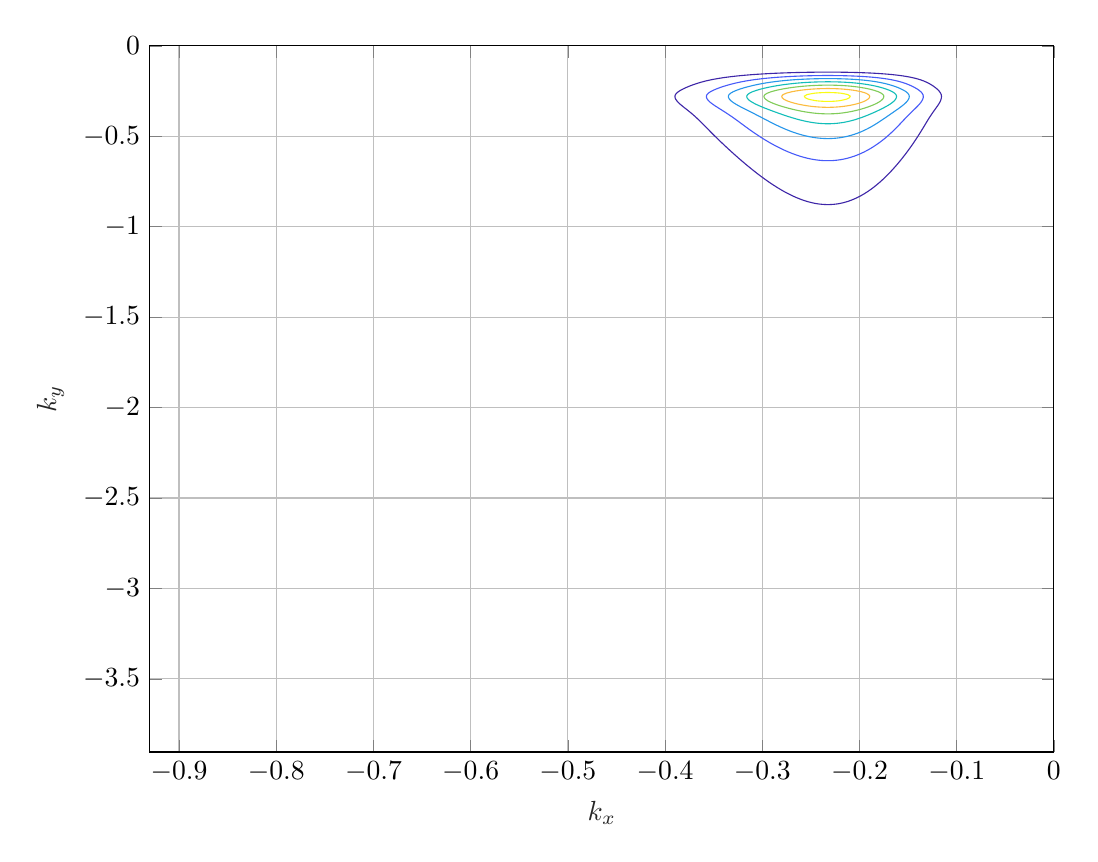
\begin{tikzpicture}

\begin{axis}[%
width=4.521in,
height=3.531in,
at={(0.758in,0.516in)},
scale only axis,
colormap={mymap}{[1pt] rgb(0pt)=(0.2422,0.1504,0.6603); rgb(1pt)=(0.2444,0.1534,0.6728); rgb(2pt)=(0.2464,0.1569,0.6847); rgb(3pt)=(0.2484,0.1607,0.6961); rgb(4pt)=(0.2503,0.1648,0.7071); rgb(5pt)=(0.2522,0.1689,0.7179); rgb(6pt)=(0.254,0.1732,0.7286); rgb(7pt)=(0.2558,0.1773,0.7393); rgb(8pt)=(0.2576,0.1814,0.7501); rgb(9pt)=(0.2594,0.1854,0.761); rgb(11pt)=(0.2628,0.1932,0.7828); rgb(12pt)=(0.2645,0.1972,0.7937); rgb(13pt)=(0.2661,0.2011,0.8043); rgb(14pt)=(0.2676,0.2052,0.8148); rgb(15pt)=(0.2691,0.2094,0.8249); rgb(16pt)=(0.2704,0.2138,0.8346); rgb(17pt)=(0.2717,0.2184,0.8439); rgb(18pt)=(0.2729,0.2231,0.8528); rgb(19pt)=(0.274,0.228,0.8612); rgb(20pt)=(0.2749,0.233,0.8692); rgb(21pt)=(0.2758,0.2382,0.8767); rgb(22pt)=(0.2766,0.2435,0.884); rgb(23pt)=(0.2774,0.2489,0.8908); rgb(24pt)=(0.2781,0.2543,0.8973); rgb(25pt)=(0.2788,0.2598,0.9035); rgb(26pt)=(0.2794,0.2653,0.9094); rgb(27pt)=(0.2798,0.2708,0.915); rgb(28pt)=(0.2802,0.2764,0.9204); rgb(29pt)=(0.2806,0.2819,0.9255); rgb(30pt)=(0.2809,0.2875,0.9305); rgb(31pt)=(0.2811,0.293,0.9352); rgb(32pt)=(0.2813,0.2985,0.9397); rgb(33pt)=(0.2814,0.304,0.9441); rgb(34pt)=(0.2814,0.3095,0.9483); rgb(35pt)=(0.2813,0.315,0.9524); rgb(36pt)=(0.2811,0.3204,0.9563); rgb(37pt)=(0.2809,0.3259,0.96); rgb(38pt)=(0.2807,0.3313,0.9636); rgb(39pt)=(0.2803,0.3367,0.967); rgb(40pt)=(0.2798,0.3421,0.9702); rgb(41pt)=(0.2791,0.3475,0.9733); rgb(42pt)=(0.2784,0.3529,0.9763); rgb(43pt)=(0.2776,0.3583,0.9791); rgb(44pt)=(0.2766,0.3638,0.9817); rgb(45pt)=(0.2754,0.3693,0.984); rgb(46pt)=(0.2741,0.3748,0.9862); rgb(47pt)=(0.2726,0.3804,0.9881); rgb(48pt)=(0.271,0.386,0.9898); rgb(49pt)=(0.2691,0.3916,0.9912); rgb(50pt)=(0.267,0.3973,0.9924); rgb(51pt)=(0.2647,0.403,0.9935); rgb(52pt)=(0.2621,0.4088,0.9946); rgb(53pt)=(0.2591,0.4145,0.9955); rgb(54pt)=(0.2556,0.4203,0.9965); rgb(55pt)=(0.2517,0.4261,0.9974); rgb(56pt)=(0.2473,0.4319,0.9983); rgb(57pt)=(0.2424,0.4378,0.9991); rgb(58pt)=(0.2369,0.4437,0.9996); rgb(59pt)=(0.2311,0.4497,0.9995); rgb(60pt)=(0.225,0.4559,0.9985); rgb(61pt)=(0.2189,0.462,0.9968); rgb(62pt)=(0.2128,0.4682,0.9948); rgb(63pt)=(0.2066,0.4743,0.9926); rgb(64pt)=(0.2006,0.4803,0.9906); rgb(65pt)=(0.195,0.4861,0.9887); rgb(66pt)=(0.1903,0.4919,0.9867); rgb(67pt)=(0.1869,0.4975,0.9844); rgb(68pt)=(0.1847,0.503,0.9819); rgb(69pt)=(0.1831,0.5084,0.9793); rgb(70pt)=(0.1818,0.5138,0.9766); rgb(71pt)=(0.1806,0.5191,0.9738); rgb(72pt)=(0.1795,0.5244,0.9709); rgb(73pt)=(0.1785,0.5296,0.9677); rgb(74pt)=(0.1778,0.5349,0.9641); rgb(75pt)=(0.1773,0.5401,0.9602); rgb(76pt)=(0.1768,0.5452,0.956); rgb(77pt)=(0.1764,0.5504,0.9516); rgb(78pt)=(0.1755,0.5554,0.9473); rgb(79pt)=(0.174,0.5605,0.9432); rgb(80pt)=(0.1716,0.5655,0.9393); rgb(81pt)=(0.1686,0.5705,0.9357); rgb(82pt)=(0.1649,0.5755,0.9323); rgb(83pt)=(0.161,0.5805,0.9289); rgb(84pt)=(0.1573,0.5854,0.9254); rgb(85pt)=(0.154,0.5902,0.9218); rgb(86pt)=(0.1513,0.595,0.9182); rgb(87pt)=(0.1492,0.5997,0.9147); rgb(88pt)=(0.1475,0.6043,0.9113); rgb(89pt)=(0.1461,0.6089,0.908); rgb(90pt)=(0.1446,0.6135,0.905); rgb(91pt)=(0.1429,0.618,0.9022); rgb(92pt)=(0.1408,0.6226,0.8998); rgb(93pt)=(0.1383,0.6272,0.8975); rgb(94pt)=(0.1354,0.6317,0.8953); rgb(95pt)=(0.1321,0.6363,0.8932); rgb(96pt)=(0.1288,0.6408,0.891); rgb(97pt)=(0.1253,0.6453,0.8887); rgb(98pt)=(0.1219,0.6497,0.8862); rgb(99pt)=(0.1185,0.6541,0.8834); rgb(100pt)=(0.1152,0.6584,0.8804); rgb(101pt)=(0.1119,0.6627,0.877); rgb(102pt)=(0.1085,0.6669,0.8734); rgb(103pt)=(0.1048,0.671,0.8695); rgb(104pt)=(0.1009,0.675,0.8653); rgb(105pt)=(0.0964,0.6789,0.8609); rgb(106pt)=(0.0914,0.6828,0.8562); rgb(107pt)=(0.0855,0.6865,0.8513); rgb(108pt)=(0.0789,0.6902,0.8462); rgb(109pt)=(0.0713,0.6938,0.8409); rgb(110pt)=(0.0628,0.6972,0.8355); rgb(111pt)=(0.0535,0.7006,0.8299); rgb(112pt)=(0.0433,0.7039,0.8242); rgb(113pt)=(0.0328,0.7071,0.8183); rgb(114pt)=(0.0234,0.7103,0.8124); rgb(115pt)=(0.0155,0.7133,0.8064); rgb(116pt)=(0.0091,0.7163,0.8003); rgb(117pt)=(0.0046,0.7192,0.7941); rgb(118pt)=(0.0019,0.722,0.7878); rgb(119pt)=(0.0009,0.7248,0.7815); rgb(120pt)=(0.0018,0.7275,0.7752); rgb(121pt)=(0.0046,0.7301,0.7688); rgb(122pt)=(0.0094,0.7327,0.7623); rgb(123pt)=(0.0162,0.7352,0.7558); rgb(124pt)=(0.0253,0.7376,0.7492); rgb(125pt)=(0.0369,0.74,0.7426); rgb(126pt)=(0.0504,0.7423,0.7359); rgb(127pt)=(0.0638,0.7446,0.7292); rgb(128pt)=(0.077,0.7468,0.7224); rgb(129pt)=(0.0899,0.7489,0.7156); rgb(130pt)=(0.1023,0.751,0.7088); rgb(131pt)=(0.1141,0.7531,0.7019); rgb(132pt)=(0.1252,0.7552,0.695); rgb(133pt)=(0.1354,0.7572,0.6881); rgb(134pt)=(0.1448,0.7593,0.6812); rgb(135pt)=(0.1532,0.7614,0.6741); rgb(136pt)=(0.1609,0.7635,0.6671); rgb(137pt)=(0.1678,0.7656,0.6599); rgb(138pt)=(0.1741,0.7678,0.6527); rgb(139pt)=(0.1799,0.7699,0.6454); rgb(140pt)=(0.1853,0.7721,0.6379); rgb(141pt)=(0.1905,0.7743,0.6303); rgb(142pt)=(0.1954,0.7765,0.6225); rgb(143pt)=(0.2003,0.7787,0.6146); rgb(144pt)=(0.2061,0.7808,0.6065); rgb(145pt)=(0.2118,0.7828,0.5983); rgb(146pt)=(0.2178,0.7849,0.5899); rgb(147pt)=(0.2244,0.7869,0.5813); rgb(148pt)=(0.2318,0.7887,0.5725); rgb(149pt)=(0.2401,0.7905,0.5636); rgb(150pt)=(0.2491,0.7922,0.5546); rgb(151pt)=(0.2589,0.7937,0.5454); rgb(152pt)=(0.2695,0.7951,0.536); rgb(153pt)=(0.2809,0.7964,0.5266); rgb(154pt)=(0.2929,0.7975,0.517); rgb(155pt)=(0.3052,0.7985,0.5074); rgb(156pt)=(0.3176,0.7994,0.4975); rgb(157pt)=(0.3301,0.8002,0.4876); rgb(158pt)=(0.3424,0.8009,0.4774); rgb(159pt)=(0.3548,0.8016,0.4669); rgb(160pt)=(0.3671,0.8021,0.4563); rgb(161pt)=(0.3795,0.8026,0.4454); rgb(162pt)=(0.3921,0.8029,0.4344); rgb(163pt)=(0.405,0.8031,0.4233); rgb(164pt)=(0.4184,0.803,0.4122); rgb(165pt)=(0.4322,0.8028,0.4013); rgb(166pt)=(0.4463,0.8024,0.3904); rgb(167pt)=(0.4608,0.8018,0.3797); rgb(168pt)=(0.4753,0.8011,0.3691); rgb(169pt)=(0.4899,0.8002,0.3586); rgb(170pt)=(0.5044,0.7993,0.348); rgb(171pt)=(0.5187,0.7982,0.3374); rgb(172pt)=(0.5329,0.797,0.3267); rgb(173pt)=(0.547,0.7957,0.3159); rgb(175pt)=(0.5748,0.7929,0.2941); rgb(176pt)=(0.5886,0.7913,0.2833); rgb(177pt)=(0.6024,0.7896,0.2726); rgb(178pt)=(0.6161,0.7878,0.2622); rgb(179pt)=(0.6297,0.7859,0.2521); rgb(180pt)=(0.6433,0.7839,0.2423); rgb(181pt)=(0.6567,0.7818,0.2329); rgb(182pt)=(0.6701,0.7796,0.2239); rgb(183pt)=(0.6833,0.7773,0.2155); rgb(184pt)=(0.6963,0.775,0.2075); rgb(185pt)=(0.7091,0.7727,0.1998); rgb(186pt)=(0.7218,0.7703,0.1924); rgb(187pt)=(0.7344,0.7679,0.1852); rgb(188pt)=(0.7468,0.7654,0.1782); rgb(189pt)=(0.759,0.7629,0.1717); rgb(190pt)=(0.771,0.7604,0.1658); rgb(191pt)=(0.7829,0.7579,0.1608); rgb(192pt)=(0.7945,0.7554,0.157); rgb(193pt)=(0.806,0.7529,0.1546); rgb(194pt)=(0.8172,0.7505,0.1535); rgb(195pt)=(0.8281,0.7481,0.1536); rgb(196pt)=(0.8389,0.7457,0.1546); rgb(197pt)=(0.8495,0.7435,0.1564); rgb(198pt)=(0.86,0.7413,0.1587); rgb(199pt)=(0.8703,0.7392,0.1615); rgb(200pt)=(0.8804,0.7372,0.165); rgb(201pt)=(0.8903,0.7353,0.1695); rgb(202pt)=(0.9,0.7336,0.1749); rgb(203pt)=(0.9093,0.7321,0.1815); rgb(204pt)=(0.9184,0.7308,0.189); rgb(205pt)=(0.9272,0.7298,0.1973); rgb(206pt)=(0.9357,0.729,0.2061); rgb(207pt)=(0.944,0.7285,0.2151); rgb(208pt)=(0.9523,0.7284,0.2237); rgb(209pt)=(0.9606,0.7285,0.2312); rgb(210pt)=(0.9689,0.7292,0.2373); rgb(211pt)=(0.977,0.7304,0.2418); rgb(212pt)=(0.9842,0.733,0.2446); rgb(213pt)=(0.99,0.7365,0.2429); rgb(214pt)=(0.9946,0.7407,0.2394); rgb(215pt)=(0.9966,0.7458,0.2351); rgb(216pt)=(0.9971,0.7513,0.2309); rgb(217pt)=(0.9972,0.7569,0.2267); rgb(218pt)=(0.9971,0.7626,0.2224); rgb(219pt)=(0.9969,0.7683,0.2181); rgb(220pt)=(0.9966,0.774,0.2138); rgb(221pt)=(0.9962,0.7798,0.2095); rgb(222pt)=(0.9957,0.7856,0.2053); rgb(223pt)=(0.9949,0.7915,0.2012); rgb(224pt)=(0.9938,0.7974,0.1974); rgb(225pt)=(0.9923,0.8034,0.1939); rgb(226pt)=(0.9906,0.8095,0.1906); rgb(227pt)=(0.9885,0.8156,0.1875); rgb(228pt)=(0.9861,0.8218,0.1846); rgb(229pt)=(0.9835,0.828,0.1817); rgb(230pt)=(0.9807,0.8342,0.1787); rgb(231pt)=(0.9778,0.8404,0.1757); rgb(232pt)=(0.9748,0.8467,0.1726); rgb(233pt)=(0.972,0.8529,0.1695); rgb(234pt)=(0.9694,0.8591,0.1665); rgb(235pt)=(0.9671,0.8654,0.1636); rgb(236pt)=(0.9651,0.8716,0.1608); rgb(237pt)=(0.9634,0.8778,0.1582); rgb(238pt)=(0.9619,0.884,0.1557); rgb(239pt)=(0.9608,0.8902,0.1532); rgb(240pt)=(0.9601,0.8963,0.1507); rgb(241pt)=(0.9596,0.9023,0.148); rgb(242pt)=(0.9595,0.9084,0.145); rgb(243pt)=(0.9597,0.9143,0.1418); rgb(244pt)=(0.9601,0.9203,0.1382); rgb(245pt)=(0.9608,0.9262,0.1344); rgb(246pt)=(0.9618,0.932,0.1304); rgb(247pt)=(0.9629,0.9379,0.1261); rgb(248pt)=(0.9642,0.9437,0.1216); rgb(249pt)=(0.9657,0.9494,0.1168); rgb(250pt)=(0.9674,0.9552,0.1116); rgb(251pt)=(0.9692,0.9609,0.1061); rgb(252pt)=(0.9711,0.9667,0.1001); rgb(253pt)=(0.973,0.9724,0.0938); rgb(254pt)=(0.9749,0.9782,0.0872); rgb(255pt)=(0.9769,0.9839,0.0805)},
xmin=-0.930195154145727,
xmax=0,
xlabel style={font=\color{white!15!black}},
xlabel={$k_{x}$},
ymin=-3.90455241197714,
ymax=0,
ylabel style={font=\color{white!15!black}},
ylabel={$k_{y}$},
axis background/.style={fill=white},
xmajorgrids,
ymajorgrids
]
\addplot[contour prepared, contour prepared format=matlab, contour/labels=false] table[row sep=crcr] {%
%
0.005	291\\
-0.196855524076637	-0.148804468836322\\
-0.198674719356596	-0.148433867867508\\
-0.202114910320485	-0.147817601337958\\
-0.205584630820544	-0.147283319880835\\
-0.209083880856774	-0.146826004027864\\
-0.212612660429175	-0.14644142234799\\
-0.216170969537747	-0.146126063608075\\
-0.219758808182489	-0.145877081252974\\
-0.223376176363402	-0.145692248928751\\
-0.227023074080486	-0.14556992603921\\
-0.230699501333741	-0.145509032561826\\
-0.234405458123166	-0.145509032561826\\
-0.238140944448762	-0.14556992603921\\
-0.241905960310528	-0.145692248928751\\
-0.245700505708466	-0.145877081252974\\
-0.249524580642574	-0.146126063608075\\
-0.253378185112853	-0.14644142234799\\
-0.257261319119302	-0.146826004027864\\
-0.261173982661922	-0.147283319880835\\
-0.265116175740713	-0.147817601337958\\
-0.269087898355675	-0.148433867867508\\
-0.271222105805323	-0.148804468836322\\
-0.273089150506807	-0.149104807550245\\
-0.27711993219411	-0.149824158172332\\
-0.281180243417584	-0.150635959419721\\
-0.285270084177229	-0.151548459180424\\
-0.289389454473044	-0.152571149054126\\
-0.29353835430503	-0.153714935316677\\
-0.297553240260792	-0.154940096664225\\
-0.297716783673187	-0.154988697633428\\
-0.301924742577514	-0.156314715300856\\
-0.306162231018012	-0.157793763577976\\
-0.310429248994681	-0.159443486906332\\
-0.31453911910122	-0.16119967656946\\
-0.314725796507521	-0.161280562510135\\
-0.319051873556531	-0.163247627065405\\
-0.323407480141712	-0.16544565909229\\
-0.327252114451645	-0.167583208552026\\
-0.327792616263064	-0.167898317448867\\
-0.332207281920586	-0.170599691153822\\
-0.33665147711428	-0.173629918284633\\
-0.337297872466221	-0.174090692611923\\
-0.341125201844143	-0.177036387569275\\
-0.345466534960891	-0.180722128749152\\
-0.345628456110178	-0.180873221784687\\
-0.350161239912383	-0.185264112153009\\
-0.352293310357913	-0.187477516963712\\
-0.354723553250759	-0.190291912618386\\
-0.35805050675298	-0.194356857255604\\
-0.359315396125306	-0.196089116464486\\
-0.363021647798467	-0.201360149624827\\
-0.363936768536024	-0.202816600288493\\
-0.367413526580762	-0.208487394071381\\
-0.368587670482912	-0.210618769986536\\
-0.371370269485799	-0.215738590595267\\
-0.373268101965971	-0.219607025448017\\
-0.374981450526961	-0.223113739196484\\
-0.3779780629852	-0.229926330649419\\
-0.378281417689195	-0.230612839875033\\
-0.381359513645215	-0.238235892630913\\
-0.382717553540601	-0.242136385597928\\
-0.384083624628014	-0.245982897464124\\
-0.386390104929891	-0.253853854374666\\
-0.387486573632172	-0.258852020168781\\
-0.388173452577456	-0.26184876336254\\
-0.389377043294675	-0.269967624427746\\
-0.389874749315474	-0.278210437570283\\
-0.389729844221555	-0.286577202790151\\
-0.389096914997133	-0.29506792008735\\
-0.388009499636901	-0.303682589461881\\
-0.387486573632172	-0.306788620687696\\
-0.386586484665742	-0.312421210913744\\
-0.384868963598134	-0.321283784442937\\
-0.382866623338682	-0.330270310049462\\
-0.382717553540601	-0.330906931919109\\
-0.380799600534545	-0.339380787733319\\
-0.378589148207348	-0.348615217494507\\
-0.3779780629852	-0.35117471046037\\
-0.376400913254779	-0.357973599333026\\
-0.374201037837619	-0.367455933248876\\
-0.373268101965971	-0.371586176913506\\
-0.372064534739705	-0.377062219242058\\
-0.369983893974356	-0.386792457312572\\
-0.368587670482912	-0.393481854733007\\
-0.367944571306966	-0.396646647460416\\
-0.365990433558918	-0.406624789685592\\
-0.364018526546915	-0.4167268839881\\
-0.363936768536024	-0.417159908765357\\
-0.362135868686593	-0.426952930367939\\
-0.360214540699268	-0.437302928825109\\
-0.359315396125306	-0.442158660529871\\
-0.358298790518745	-0.447776879359611\\
-0.3563690199839	-0.458374781971444\\
-0.354723553250759	-0.467221757102483\\
-0.354381364869922	-0.469096636660608\\
-0.352401999488538	-0.479942443427104\\
-0.350333380855871	-0.490912202270931\\
-0.350161239912383	-0.491826386211798\\
-0.348271022203739	-0.502005913192089\\
-0.34612242741626	-0.513223576190579\\
-0.345628456110178	-0.515792438892124\\
-0.343956898785391	-0.524565191266401\\
-0.341716641755384	-0.536030758419553\\
-0.341125201844143	-0.539045030714727\\
-0.339449944008873	-0.547620277650037\\
-0.337108764257676	-0.559333748957853\\
-0.33665147711428	-0.561620832228334\\
-0.334741187145012	-0.571171172343\\
-0.332289664043878	-0.583132547805478\\
-0.332207281920586	-0.583537339335937\\
-0.329817841011296	-0.595217875345287\\
-0.327792616263064	-0.604909596975648\\
-0.327261323684509	-0.607427154962428\\
-0.324661100549576	-0.6197603866569\\
-0.323407480141712	-0.625653932759719\\
-0.321990651064844	-0.632217570428704\\
-0.319244792399452	-0.644798706277839\\
-0.319051873556531	-0.645689511016548\\
-0.316442612535861	-0.657503794204306\\
-0.314725796507521	-0.66519911681604\\
-0.31355182540106	-0.670332834208104\\
-0.310575062176663	-0.683285826289233\\
-0.310429248994681	-0.683926322226188\\
-0.307512020708161	-0.696362770447694\\
-0.306162231018012	-0.702096889863331\\
-0.304341183342933	-0.709563666683486\\
-0.301924742577514	-0.719467560925802\\
-0.301054927994755	-0.722888514996609\\
-0.297716783673187	-0.73605183071751\\
-0.297640872845205	-0.736337315387063\\
-0.29407261737457	-0.74991006785485\\
-0.29353835430503	-0.751955516225179\\
-0.290326752974816	-0.763606772399967\\
-0.289389454473044	-0.767036452644243\\
-0.286371311032162	-0.777427429022416\\
-0.285270084177229	-0.781262510564789\\
-0.282160893471094	-0.791372037722196\\
-0.281180243417584	-0.794606641339117\\
-0.277632131274088	-0.805440598499308\\
-0.27711993219411	-0.807031638078997\\
-0.273089150506807	-0.818546853252477\\
-0.272671653302337	-0.819633111353751\\
-0.269087898355675	-0.829172796395043\\
-0.267084087910637	-0.833949576285525\\
-0.265116175740713	-0.838762426158114\\
-0.261173982661922	-0.847293473774731\\
-0.260596261761032	-0.848389993294631\\
-0.257261319119302	-0.854920297723456\\
-0.253378185112853	-0.861382357862224\\
-0.252246285753978	-0.862954362381068\\
-0.249524580642574	-0.866875807813234\\
-0.245700505708466	-0.871277784427371\\
-0.241905960310528	-0.874545596591965\\
-0.238140944448762	-0.876708249840691\\
-0.234899910151014	-0.877642683544837\\
-0.234405458123166	-0.877792238657428\\
-0.230699501333741	-0.877792238657428\\
-0.230212866729258	-0.877642683544837\\
-0.227023074080486	-0.876708249840691\\
-0.223376176363402	-0.874545596591965\\
-0.219758808182489	-0.871277784427371\\
-0.216170969537747	-0.866875807813234\\
-0.213657824204994	-0.862954362381068\\
-0.212612660429175	-0.861382357862224\\
-0.209083880856774	-0.854920297723456\\
-0.206101309513038	-0.848389993294631\\
-0.205584630820544	-0.847293473774731\\
-0.202114910320485	-0.838762426158114\\
-0.200410361861034	-0.833949576285525\\
-0.198674719356596	-0.829172796395043\\
-0.195619931929736	-0.819633111353751\\
-0.195264057928878	-0.818546853252477\\
-0.191882926037331	-0.807031638078997\\
-0.191460128978586	-0.805440598499308\\
-0.188531323681954	-0.794606641339117\\
-0.187734766779284	-0.791372037722196\\
-0.185209250862748	-0.781262510564789\\
-0.184329058788734	-0.777427429022416\\
-0.181916707579713	-0.767036452644242\\
-0.181179543989352	-0.763606772399967\\
-0.178653693832849	-0.751955516225179\\
-0.17824025350695	-0.74991006785485\\
-0.175478953337095	-0.736337315387063\\
-0.175420209622155	-0.73605183071751\\
-0.172878534822926	-0.722888514996609\\
-0.172216254947632	-0.719467560925802\\
-0.170406029287127	-0.709563666683486\\
-0.16904182980928	-0.702096889863331\\
-0.168047002113772	-0.696362770447694\\
-0.165896934207098	-0.683926322226188\\
-0.165791207123256	-0.683285826289233\\
-0.163632798049896	-0.670332834208104\\
-0.162781568141087	-0.66519911681604\\
-0.161556945103807	-0.657503794204306\\
-0.159695731611247	-0.645689511016547\\
-0.159560361440113	-0.644798706277839\\
-0.157633606376601	-0.632217570428704\\
-0.156639424617578	-0.625653932759718\\
-0.155774131070062	-0.6197603866569\\
-0.153979364259755	-0.607427154962428\\
-0.153612647160079	-0.604909596975648\\
-0.152237661795895	-0.595217875345287\\
-0.150615399238751	-0.583537339335937\\
-0.150560386591636	-0.583132547805478\\
-0.14892332299254	-0.571171172343\\
-0.147647680853594	-0.561620832228333\\
-0.147347350353475	-0.559333748957853\\
-0.145809743850214	-0.547620277650037\\
-0.144709492004607	-0.539045030714727\\
-0.144327479996363	-0.536030758419553\\
-0.14288049430813	-0.524565191266401\\
-0.141800832691792	-0.515792438892124\\
-0.141487072415941	-0.513223576190579\\
-0.140122329798488	-0.502005913192089\\
-0.138921702915147	-0.491826386211798\\
-0.138814184461771	-0.490912202270931\\
-0.137522134636189	-0.479942443427104\\
-0.136285831986976	-0.469096636660608\\
-0.136072102674672	-0.467221757102482\\
-0.135061542719593	-0.458374781971444\\
-0.1338763781789	-0.447776879359611\\
-0.133252031970369	-0.442158660529871\\
-0.132709098026347	-0.437302928825109\\
-0.131548935120263	-0.426952930367939\\
-0.130461490802236	-0.417159908765357\\
-0.130412955094183	-0.4167268839881\\
-0.129242330931502	-0.406624789685592\\
-0.12808225550647	-0.396646647460416\\
-0.127700479170273	-0.393481854733007\\
-0.126885648426055	-0.386792457312572\\
-0.12567139435164	-0.377062219242058\\
-0.124968997074482	-0.371586176913505\\
-0.124433801887925	-0.367455933248876\\
-0.123171804391561	-0.357973599333026\\
-0.122267044514861	-0.35117471046037\\
-0.121922476212031	-0.348615217494507\\
-0.120676084089842	-0.339380787733319\\
-0.119594621491411	-0.330906931919108\\
-0.119512010055323	-0.330270310049462\\
-0.118402353998227	-0.321283784442937\\
-0.117450538917417	-0.312421210913744\\
-0.116951728004132	-0.306788620687696\\
-0.116666934456941	-0.303682589461881\\
-0.116074711322292	-0.29506792008735\\
-0.115730008329299	-0.286577202790151\\
-0.115651090785841	-0.278210437570283\\
-0.115922149141784	-0.269967624427746\\
-0.116577643163162	-0.26184876336254\\
-0.116951728004132	-0.258852020168781\\
-0.117559368554313	-0.253853854374666\\
-0.118837572808294	-0.245982897464124\\
-0.119594621491411	-0.242136385597929\\
-0.120360369843638	-0.238235892630913\\
-0.122095994043138	-0.230612839875033\\
-0.122267044514861	-0.229926330649419\\
-0.123986104326328	-0.223113739196484\\
-0.124968997074482	-0.219607025448017\\
-0.126076564925686	-0.215738590595267\\
-0.127700479170273	-0.210618769986537\\
-0.128397510629645	-0.208487394071381\\
-0.130461490802236	-0.202816600288493\\
-0.131014071694882	-0.201360149624827\\
-0.133252031970369	-0.196089116464486\\
-0.134028861134723	-0.194356857255604\\
-0.136072102674672	-0.190291912618386\\
-0.137590021374735	-0.187477516963712\\
-0.138921702915147	-0.185264112153009\\
-0.141800832691792	-0.180873221784687\\
-0.141905417827561	-0.180722128749152\\
-0.144709492004607	-0.177036387569275\\
-0.147223150572946	-0.174090692611923\\
-0.147647680853594	-0.173629918284633\\
-0.150615399238751	-0.170599691153822\\
-0.153612647160079	-0.167898317448867\\
-0.153985720800958	-0.167583208552026\\
-0.156639424617578	-0.16544565909229\\
-0.159695731611247	-0.163247627065405\\
-0.162781568141087	-0.161280562510135\\
-0.162916925298233	-0.16119967656946\\
-0.165896934207098	-0.159443486906332\\
-0.16904182980928	-0.157793763577976\\
-0.172216254947632	-0.156314715300856\\
-0.175420209622155	-0.154988697633428\\
-0.175546767951888	-0.154940096664225\\
-0.178653693832849	-0.153714935316677\\
-0.181916707579713	-0.152571149054126\\
-0.185209250862748	-0.151548459180424\\
-0.188531323681954	-0.150635959419721\\
-0.191882926037331	-0.149824158172332\\
-0.195264057928878	-0.149104807550245\\
-0.196855524076637	-0.148804468836322\\
0.01	221\\
-0.204089990128102	-0.167583208552026\\
-0.205584630820544	-0.167218882689699\\
-0.209083880856774	-0.166485513857602\\
-0.212612660429175	-0.165868784269982\\
-0.216170969537747	-0.165363063181853\\
-0.219758808182489	-0.16496378575076\\
-0.223376176363402	-0.164667381712132\\
-0.227023074080486	-0.164471220144456\\
-0.230699501333741	-0.164373569083158\\
-0.234405458123166	-0.164373569083158\\
-0.238140944448762	-0.164471220144456\\
-0.241905960310528	-0.164667381712132\\
-0.245700505708466	-0.16496378575076\\
-0.249524580642574	-0.165363063181853\\
-0.253378185112853	-0.165868784269982\\
-0.257261319119302	-0.166485513857602\\
-0.261173982661922	-0.167218882689699\\
-0.262872148895463	-0.167583208552026\\
-0.265116175740713	-0.168066252699074\\
-0.269087898355675	-0.169035609526974\\
-0.273089150506807	-0.170143188319726\\
-0.27711993219411	-0.171399774174091\\
-0.281180243417584	-0.172817855889325\\
-0.284470172642135	-0.174090692611923\\
-0.285270084177229	-0.174412037444747\\
-0.289389454473044	-0.176199598422342\\
-0.29353835430503	-0.178198823937543\\
-0.297716783673187	-0.180431601456792\\
-0.298228986807371	-0.180722128749152\\
-0.301924742577514	-0.182956929066661\\
-0.306162231018012	-0.18577868227302\\
-0.308523207559827	-0.187477516963712\\
-0.310429248994681	-0.188960796527956\\
-0.314725796507521	-0.192556732638394\\
-0.316730651067302	-0.194356857255604\\
-0.319051873556531	-0.196628013938362\\
-0.323407480141712	-0.20122875595073\\
-0.323526952683711	-0.201360149624827\\
-0.327792616263064	-0.206478524097554\\
-0.329370113272455	-0.208487394071381\\
-0.332207281920586	-0.212406814423409\\
-0.334506185326786	-0.215738590595267\\
-0.33665147711428	-0.219095158965312\\
-0.339123927902316	-0.223113739196484\\
-0.341125201844143	-0.226633807786818\\
-0.343322659406662	-0.230612839875033\\
-0.345628456110178	-0.235205105959218\\
-0.34712043165907	-0.238235892630913\\
-0.350161239912383	-0.245280834883703\\
-0.350461503037606	-0.245982897464124\\
-0.353308332547513	-0.253853854374666\\
-0.354723553250759	-0.259086882558368\\
-0.355481780738441	-0.26184876336254\\
-0.356925121700895	-0.269967624427746\\
-0.357521968682848	-0.278210437570283\\
-0.357348199099277	-0.286577202790151\\
-0.356589193016167	-0.29506792008735\\
-0.355285169056718	-0.303682589461881\\
-0.354723553250759	-0.306467690681803\\
-0.353550719021274	-0.312421210913744\\
-0.351430826796234	-0.321283784442937\\
-0.350161239912383	-0.325999981810127\\
-0.349020587202476	-0.330270310049462\\
-0.346409003644198	-0.339380787733319\\
-0.345628456110178	-0.342037977169414\\
-0.343695354871991	-0.348615217494507\\
-0.341125201844143	-0.357228574374069\\
-0.340901822513782	-0.357973599333026\\
-0.338146451362843	-0.367455933248876\\
-0.33665147711428	-0.372711844083202\\
-0.335405819887601	-0.377062219242058\\
-0.332709708666971	-0.386792457312572\\
-0.332207281920586	-0.388688533497818\\
-0.330082350732401	-0.396646647460416\\
-0.327792616263064	-0.405408136891623\\
-0.327471216630879	-0.406624789685592\\
-0.324904412199593	-0.4167268839881\\
-0.323407480141712	-0.422693008355968\\
-0.322324211511001	-0.426952930367939\\
-0.31972179197521	-0.437302928825109\\
-0.319051873556531	-0.439994651252416\\
-0.317080868155977	-0.447776879359611\\
-0.314725796507521	-0.456991820026865\\
-0.314364297807172	-0.458374781971444\\
-0.311574761806662	-0.469096636660608\\
-0.310429248994681	-0.473463888399764\\
-0.308681475617418	-0.479942443427104\\
-0.306162231018012	-0.489173268075743\\
-0.305671252620898	-0.490912202270931\\
-0.302533272495481	-0.502005913192089\\
-0.301924742577514	-0.504151200529747\\
-0.299245230226036	-0.513223576190579\\
-0.297716783673187	-0.518370561666152\\
-0.295788918317463	-0.524565191266401\\
-0.29353835430503	-0.531784147201311\\
-0.29214125593058	-0.536030758419553\\
-0.289389454473044	-0.544412141696058\\
-0.288269651930774	-0.547620277650037\\
-0.285270084177229	-0.556263773426203\\
-0.28412831207742	-0.559333748957853\\
-0.281180243417584	-0.567336267190073\\
-0.279652795586088	-0.571171172343\\
-0.27711993219411	-0.577614576536799\\
-0.27475164815669	-0.583132547805478\\
-0.273089150506807	-0.587071378449766\\
-0.26929302115733	-0.595217875345287\\
-0.269087898355675	-0.595667047275528\\
-0.265116175740713	-0.603544820128684\\
-0.262897202877986	-0.607427154962428\\
-0.261173982661922	-0.610522882704594\\
-0.257261319119302	-0.616662936631505\\
-0.254947771350379	-0.6197603866569\\
-0.253378185112853	-0.621931397163592\\
-0.249524580642574	-0.626380588210412\\
-0.245700505708466	-0.629893318079344\\
-0.242321511202533	-0.632217570428704\\
-0.241905960310528	-0.632515512795357\\
-0.238140944448762	-0.634329673244236\\
-0.234405458123166	-0.635232779266986\\
-0.230699501333741	-0.635232779266986\\
-0.227023074080486	-0.634329673244236\\
-0.223376176363402	-0.632515512795357\\
-0.222980028625888	-0.632217570428704\\
-0.219758808182489	-0.629893318079344\\
-0.216170969537747	-0.626380588210412\\
-0.212612660429175	-0.621931397163592\\
-0.211186306395834	-0.6197603866569\\
-0.209083880856774	-0.616662936631505\\
-0.205584630820544	-0.610522882704594\\
-0.204067938870076	-0.607427154962428\\
-0.202114910320485	-0.603544820128684\\
-0.198674719356596	-0.595667047275528\\
-0.19849987298323	-0.595217875345287\\
-0.195264057928878	-0.587071378449766\\
-0.193869508618171	-0.583132547805478\\
-0.191882926037331	-0.577614576536799\\
-0.189792162437408	-0.571171172343\\
-0.188531323681954	-0.567336267190073\\
-0.186136683073784	-0.559333748957853\\
-0.185209250862748	-0.556263773426203\\
-0.182811746887693	-0.547620277650037\\
-0.181916707579713	-0.544412141696057\\
-0.179752479387131	-0.536030758419553\\
-0.178653693832849	-0.531784147201311\\
-0.176912091293192	-0.524565191266401\\
-0.175420209622155	-0.518370561666152\\
-0.174256445053845	-0.513223576190579\\
-0.172216254947632	-0.504151200529746\\
-0.171760387587483	-0.502005913192089\\
-0.169409635925585	-0.490912202270931\\
-0.16904182980928	-0.489173268075743\\
-0.167185085519753	-0.479942443427104\\
-0.165896934207098	-0.473463888399764\\
-0.165066339006658	-0.469096636660608\\
-0.16304368575543	-0.458374781971444\\
-0.162781568141087	-0.456991820026865\\
-0.161101670617104	-0.447776879359611\\
-0.159695731611247	-0.439994651252416\\
-0.159225653263225	-0.437302928825109\\
-0.157399548707602	-0.426952930367939\\
-0.156639424617578	-0.422693008355967\\
-0.155606188685371	-0.4167268839881\\
-0.153834488657042	-0.406624789685592\\
-0.153612647160079	-0.405408136891623\\
-0.152058078272871	-0.396646647460416\\
-0.150615399238751	-0.388688533497818\\
-0.150279891677212	-0.386792457312572\\
-0.148479498470081	-0.377062219242058\\
-0.147647680853594	-0.372711844083201\\
-0.146665833079785	-0.367455933248876\\
-0.144856199881644	-0.357973599333026\\
-0.144709492004607	-0.357228574374069\\
-0.143049425950555	-0.348615217494507\\
-0.141800832691792	-0.342037977169414\\
-0.141305045170183	-0.339380787733319\\
-0.139646221737401	-0.330270310049462\\
-0.138921702915147	-0.325999981810127\\
-0.138128724699667	-0.321283784442937\\
-0.136804649620597	-0.312421210913744\\
-0.136072102674672	-0.306467690681803\\
-0.135727187501238	-0.303682589461881\\
-0.134926323911994	-0.29506792008735\\
-0.1344601819124	-0.286577202790151\\
-0.134353461685834	-0.278210437570283\\
-0.13472001401237	-0.269967624427746\\
-0.135606438847833	-0.26184876336254\\
-0.136072102674672	-0.259086882558368\\
-0.136956043113917	-0.253853854374666\\
-0.138734159927548	-0.245982897464124\\
-0.138921702915147	-0.245280834883704\\
-0.140853160926209	-0.238235892630913\\
-0.141800832691792	-0.235205105959218\\
-0.143290150562587	-0.230612839875033\\
-0.144709492004607	-0.226633807786818\\
-0.146023860039009	-0.223113739196484\\
-0.147647680853594	-0.219095158965312\\
-0.149080251117003	-0.215738590595267\\
-0.150615399238751	-0.212406814423409\\
-0.152541637484807	-0.208487394071381\\
-0.153612647160079	-0.206478524097554\\
-0.156556960405087	-0.201360149624827\\
-0.156639424617578	-0.20122875595073\\
-0.159695731611247	-0.196628013938362\\
-0.161351484171824	-0.194356857255604\\
-0.162781568141087	-0.192556732638394\\
-0.165896934207098	-0.188960796527956\\
-0.167301732911679	-0.187477516963712\\
-0.16904182980928	-0.18577868227302\\
-0.172216254947632	-0.182956929066661\\
-0.175030216358583	-0.180722128749152\\
-0.175420209622155	-0.180431601456792\\
-0.178653693832849	-0.178198823937543\\
-0.181916707579713	-0.176199598422342\\
-0.185209250862748	-0.174412037444747\\
-0.185858998499558	-0.174090692611923\\
-0.188531323681954	-0.172817855889325\\
-0.191882926037331	-0.171399774174091\\
-0.195264057928878	-0.170143188319726\\
-0.198674719356596	-0.169035609526974\\
-0.202114910320485	-0.168066252699074\\
-0.204089990128102	-0.167583208552026\\
0.015	173\\
-0.200806596518139	-0.187477516963712\\
-0.202114910320485	-0.186924544936955\\
-0.205584630820544	-0.185643764417515\\
-0.209083880856774	-0.184547485989904\\
-0.212612660429175	-0.183625566059597\\
-0.216170969537747	-0.182869587491871\\
-0.219758808182489	-0.182272726519353\\
-0.223376176363402	-0.181829646122173\\
-0.227023074080486	-0.18153641346003\\
-0.230699501333741	-0.181390439500885\\
-0.234405458123166	-0.181390439500885\\
-0.238140944448762	-0.18153641346003\\
-0.241905960310528	-0.181829646122173\\
-0.245700505708466	-0.182272726519353\\
-0.249524580642574	-0.182869587491871\\
-0.253378185112853	-0.183625566059597\\
-0.257261319119302	-0.184547485989904\\
-0.261173982661922	-0.185643764417515\\
-0.265116175740713	-0.186924544936955\\
-0.266626632448143	-0.187477516963712\\
-0.269087898355675	-0.188424031362211\\
-0.273089150506807	-0.190152486433183\\
-0.27711993219411	-0.192113477566544\\
-0.281180243417584	-0.194326494417163\\
-0.281232023051579	-0.194356857255604\\
-0.285270084177229	-0.196876836120384\\
-0.289389454473044	-0.199736017627982\\
-0.29154108648535	-0.201360149624827\\
-0.29353835430503	-0.20296613342925\\
-0.297716783673187	-0.206610918630126\\
-0.29970930286236	-0.208487394071381\\
-0.301924742577514	-0.210703450941443\\
-0.306162231018012	-0.215292633685827\\
-0.306552955041759	-0.215738590595267\\
-0.310429248994681	-0.220428372254625\\
-0.31250388305249	-0.223113739196484\\
-0.314725796507521	-0.226169299056331\\
-0.317776146884247	-0.230612839875033\\
-0.319051873556531	-0.232619287280924\\
-0.322457070581489	-0.238235892630913\\
-0.323407480141712	-0.239990642765517\\
-0.326537211925288	-0.245982897464124\\
-0.327792616263064	-0.248849373614177\\
-0.329934664004851	-0.253853854374666\\
-0.332207281920586	-0.260881651430764\\
-0.332517865951021	-0.26184876336254\\
-0.334221894446989	-0.269967624427746\\
-0.334926540328618	-0.278210437570283\\
-0.33472138553163	-0.286577202790151\\
-0.333825292350686	-0.29506792008735\\
-0.332285743453973	-0.303682589461881\\
-0.332207281920586	-0.304015211228586\\
-0.330227176635983	-0.312421210913744\\
-0.327792616263064	-0.320871093620102\\
-0.327672530488905	-0.321283784442937\\
-0.324777864422751	-0.330270310049462\\
-0.323407480141712	-0.334249765309064\\
-0.32160087481259	-0.339380787733319\\
-0.319051873556531	-0.346426602342789\\
-0.318237326506687	-0.348615217494507\\
-0.314768250215996	-0.357973599333026\\
-0.314725796507521	-0.358092045392337\\
-0.311259294581549	-0.367455933248876\\
-0.310429248994681	-0.369779918511418\\
-0.307732666825044	-0.377062219242058\\
-0.306162231018012	-0.381490202134391\\
-0.304205178335486	-0.386792457312572\\
-0.301924742577514	-0.393254845263331\\
-0.300673962484034	-0.396646647460416\\
-0.297716783673187	-0.405014759657316\\
-0.29711939683823	-0.406624789685592\\
-0.29353835430503	-0.416645964465345\\
-0.293507827366014	-0.4167268839881\\
-0.289784484905512	-0.426952930367939\\
-0.289389454473044	-0.428063026580896\\
-0.285898310037783	-0.437302928825109\\
-0.285270084177229	-0.438995475089166\\
-0.281783066521443	-0.447776879359611\\
-0.281180243417584	-0.449317309479739\\
-0.277355525330051	-0.458374781971444\\
-0.27711993219411	-0.458940090718023\\
-0.273089150506807	-0.467855652233304\\
-0.272472227573532	-0.469096636660608\\
-0.269087898355675	-0.476015431972419\\
-0.266944064510422	-0.479942443427104\\
-0.265116175740713	-0.483350096399213\\
-0.261173982661922	-0.489858908562657\\
-0.260446061607413	-0.490912202270931\\
-0.257261319119302	-0.49562667722122\\
-0.253378185112853	-0.50051564751415\\
-0.251958372701121	-0.502005913192089\\
-0.249524580642574	-0.504634599063844\\
-0.245700505708466	-0.507937971139134\\
-0.241905960310528	-0.510390233020114\\
-0.238140944448762	-0.512013151308102\\
-0.234405458123166	-0.512821055196217\\
-0.230699501333741	-0.512821055196217\\
-0.227023074080486	-0.512013151308102\\
-0.223376176363402	-0.510390233020114\\
-0.219758808182489	-0.507937971139134\\
-0.216170969537747	-0.504634599063843\\
-0.213923674954951	-0.502005913192089\\
-0.212612660429175	-0.50051564751415\\
-0.209083880856774	-0.49562667722122\\
-0.206235639461747	-0.490912202270931\\
-0.205584630820544	-0.489858908562657\\
-0.202114910320485	-0.483350096399213\\
-0.200531646070142	-0.479942443427104\\
-0.198674719356596	-0.476015431972419\\
-0.195789922126615	-0.469096636660608\\
-0.195264057928878	-0.467855652233304\\
-0.191882926037331	-0.458940090718023\\
-0.191688454612391	-0.458374781971444\\
-0.188531323681954	-0.449317309479739\\
-0.188041665926112	-0.447776879359611\\
-0.185209250862748	-0.438995475089166\\
-0.184707120515424	-0.437302928825109\\
-0.181916707579713	-0.428063026580896\\
-0.181606025282292	-0.426952930367939\\
-0.178677702564246	-0.4167268839881\\
-0.178653693832849	-0.416645964465345\\
-0.175882498374295	-0.406624789685592\\
-0.175420209622155	-0.405014759657316\\
-0.17316860329951	-0.396646647460416\\
-0.172216254947632	-0.393254845263331\\
-0.170507914571451	-0.386792457312572\\
-0.16904182980928	-0.381490202134391\\
-0.16788438058126	-0.377062219242058\\
-0.165896934207098	-0.369779918511418\\
-0.16529507984686	-0.367455933248876\\
-0.162781568141087	-0.358092045392337\\
-0.162751285461663	-0.357973599333026\\
-0.160276756639976	-0.348615217494507\\
-0.159695731611247	-0.346426602342789\\
-0.157907110390894	-0.339380787733319\\
-0.156639424617578	-0.334249765309064\\
-0.155693536477467	-0.330270310049462\\
-0.153695534647293	-0.321283784442937\\
-0.153612647160079	-0.320871093620102\\
-0.151959751656057	-0.312421210913744\\
-0.150615399238751	-0.304015211228586\\
-0.150563004659978	-0.303682589461881\\
-0.14953493380204	-0.29506792008735\\
-0.148936545996825	-0.286577202790151\\
-0.1487995489397	-0.278210437570283\\
-0.149270093199526	-0.269967624427746\\
-0.150407999271584	-0.26184876336254\\
-0.150615399238751	-0.260881651430764\\
-0.15215834718823	-0.253853854374666\\
-0.153612647160079	-0.248849373614177\\
-0.154479172039689	-0.245982897464124\\
-0.156639424617578	-0.239990642765517\\
-0.157306322173396	-0.238235892630913\\
-0.159695731611247	-0.232619287280924\\
-0.160605720944037	-0.230612839875033\\
-0.162781568141087	-0.226169299056331\\
-0.16439264628202	-0.223113739196484\\
-0.165896934207098	-0.220428372254625\\
-0.168753856739875	-0.215738590595267\\
-0.16904182980928	-0.215292633685827\\
-0.172216254947632	-0.210703450941443\\
-0.173903098520224	-0.208487394071381\\
-0.175420209622155	-0.206610918630126\\
-0.178653693832849	-0.20296613342925\\
-0.180224498772882	-0.201360149624827\\
-0.181916707579713	-0.199736017627982\\
-0.185209250862748	-0.196876836120384\\
-0.188489264412464	-0.194356857255604\\
-0.188531323681954	-0.194326494417163\\
-0.191882926037331	-0.192113477566544\\
-0.195264057928878	-0.190152486433183\\
-0.198674719356596	-0.188424031362211\\
-0.200806596518139	-0.187477516963712\\
0.02	139\\
-0.215137799195968	-0.201360149624827\\
-0.216170969537747	-0.201055872903282\\
-0.219758808182489	-0.200220137832385\\
-0.223376176363402	-0.199599728986439\\
-0.227023074080486	-0.19918913953434\\
-0.230699501333741	-0.198984744268587\\
-0.234405458123166	-0.198984744268587\\
-0.238140944448762	-0.19918913953434\\
-0.241905960310528	-0.199599728986439\\
-0.245700505708466	-0.200220137832385\\
-0.249524580642574	-0.201055872903282\\
-0.250643491261679	-0.201360149624827\\
-0.253378185112853	-0.202129927279943\\
-0.257261319119302	-0.203447377687883\\
-0.261173982661922	-0.205013991462237\\
-0.265116175740713	-0.20684426409476\\
-0.268224801831597	-0.208487394071381\\
-0.269087898355675	-0.208960834556365\\
-0.273089150506807	-0.211401048772474\\
-0.27711993219411	-0.214169554891991\\
-0.279193663924761	-0.215738590595267\\
-0.281180243417584	-0.217299521838457\\
-0.285270084177229	-0.220824151394784\\
-0.287697636321962	-0.223113739196484\\
-0.289389454473044	-0.224779239068886\\
-0.29353835430503	-0.229210105690629\\
-0.294762031345597	-0.230612839875033\\
-0.297716783673187	-0.234215731194853\\
-0.300773015649049	-0.238235892630913\\
-0.301924742577514	-0.239906488270036\\
-0.305857060064278	-0.245982897464124\\
-0.306162231018012	-0.246536851374524\\
-0.310001235670234	-0.253853854374666\\
-0.310429248994681	-0.254917363928781\\
-0.313131458242229	-0.26184876336254\\
-0.314725796507521	-0.268266279401255\\
-0.315143237265334	-0.269967624427746\\
-0.315985120792274	-0.278210437570283\\
-0.315740009810204	-0.286577202790151\\
-0.314725796507521	-0.294626771351508\\
-0.314670233355787	-0.29506792008735\\
-0.312858261738131	-0.303682589461881\\
-0.310429248994681	-0.312165170132298\\
-0.310354187581503	-0.312421210913744\\
-0.307267299105819	-0.321283784442937\\
-0.306162231018012	-0.324129023300892\\
-0.303678640495373	-0.330270310049462\\
-0.301924742577514	-0.334380868837949\\
-0.299683932753385	-0.339380787733319\\
-0.297716783673187	-0.343717133961513\\
-0.295365456693589	-0.348615217494507\\
-0.29353835430503	-0.352491612001544\\
-0.290786001164932	-0.357973599333026\\
-0.289389454473044	-0.360868040273068\\
-0.28598259271957	-0.367455933248876\\
-0.285270084177229	-0.36890954391261\\
-0.281180243417584	-0.376660705418497\\
-0.280951312923443	-0.377062219242058\\
-0.27711993219411	-0.384223629049081\\
-0.275612857029542	-0.386792457312572\\
-0.273089150506807	-0.391384751641412\\
-0.269888682092611	-0.396646647460416\\
-0.269087898355675	-0.398048747581559\\
-0.265116175740713	-0.404321431981825\\
-0.263468222667355	-0.406624789685592\\
-0.261173982661922	-0.410032203069961\\
-0.257261319119302	-0.415091738221031\\
-0.255784579801413	-0.4167268839881\\
-0.253378185112853	-0.419548664208122\\
-0.249524580642574	-0.423306798272783\\
-0.245700505708466	-0.426273924125879\\
-0.244537613046369	-0.426952930367939\\
-0.241905960310528	-0.428579619378918\\
-0.238140944448762	-0.430135930686277\\
-0.234405458123166	-0.430910676997067\\
-0.230699501333741	-0.430910676997067\\
-0.227023074080486	-0.430135930686277\\
-0.223376176363402	-0.428579619378918\\
-0.220867402354527	-0.426952930367939\\
-0.219758808182489	-0.426273924125879\\
-0.216170969537747	-0.423306798272783\\
-0.212612660429175	-0.419548664208122\\
-0.210425860693184	-0.4167268839881\\
-0.209083880856774	-0.415091738221031\\
-0.205584630820544	-0.410032203069961\\
-0.203565355909395	-0.406624789685592\\
-0.202114910320485	-0.404321431981825\\
-0.198674719356596	-0.398048747581559\\
-0.197992132481201	-0.396646647460416\\
-0.195264057928878	-0.391384751641412\\
-0.193147102640577	-0.386792457312572\\
-0.191882926037331	-0.384223629049081\\
-0.188720295398936	-0.377062219242058\\
-0.188531323681954	-0.376660705418497\\
-0.185209250862748	-0.36890954391261\\
-0.184639754787687	-0.367455933248876\\
-0.181916707579713	-0.360868040273067\\
-0.180818355911004	-0.357973599333026\\
-0.178653693832849	-0.352491612001544\\
-0.177239787744176	-0.348615217494507\\
-0.175420209622155	-0.343717133961513\\
-0.173922415410215	-0.339380787733319\\
-0.172216254947632	-0.334380868837949\\
-0.170902359294881	-0.330270310049462\\
-0.16904182980928	-0.324129023300891\\
-0.168227367862211	-0.321283784442937\\
-0.165952256286707	-0.312421210913744\\
-0.165896934207098	-0.312165170132298\\
-0.164135691290026	-0.303682589461881\\
-0.162821856199561	-0.29506792008735\\
-0.162781568141087	-0.294626771351508\\
-0.162058119061699	-0.286577202790151\\
-0.161883278804864	-0.278210437570283\\
-0.16248380323193	-0.269967624427746\\
-0.162781568141087	-0.268266279401255\\
-0.163937600354065	-0.26184876336254\\
-0.165896934207098	-0.254917363928781\\
-0.166212390394321	-0.253853854374666\\
-0.16904182980928	-0.246536851374525\\
-0.169270442196224	-0.245982897464124\\
-0.172216254947632	-0.239906488270036\\
-0.173093183872113	-0.238235892630913\\
-0.175420209622155	-0.234215731194853\\
-0.177706749409229	-0.230612839875033\\
-0.178653693832849	-0.229210105690629\\
-0.181916707579713	-0.224779239068886\\
-0.183268949327711	-0.223113739196484\\
-0.185209250862748	-0.220824151394784\\
-0.188531323681954	-0.217299521838457\\
-0.190171154754212	-0.215738590595267\\
-0.191882926037331	-0.214169554891991\\
-0.195264057928878	-0.211401048772474\\
-0.198674719356596	-0.208960834556365\\
-0.199422308539161	-0.208487394071381\\
-0.202114910320485	-0.20684426409476\\
-0.205584630820544	-0.205013991462237\\
-0.209083880856774	-0.203447377687883\\
-0.212612660429175	-0.202129927279943\\
-0.215137799195968	-0.201360149624827\\
0.025	105\\
-0.20930227003982	-0.223113739196484\\
-0.212612660429175	-0.221546851632575\\
-0.216170969537747	-0.220175783130565\\
-0.219758808182489	-0.219093295723601\\
-0.223376176363402	-0.218289710010506\\
-0.227023074080486	-0.217757893258036\\
-0.230699501333741	-0.217493149909425\\
-0.234405458123166	-0.217493149909425\\
-0.238140944448762	-0.217757893258036\\
-0.241905960310528	-0.218289710010506\\
-0.245700505708466	-0.219093295723601\\
-0.249524580642574	-0.220175783130565\\
-0.253378185112853	-0.221546851632575\\
-0.257020999641725	-0.223113739196484\\
-0.257261319119302	-0.223219183269771\\
-0.261173982661922	-0.225213222141268\\
-0.265116175740713	-0.227542854903621\\
-0.269087898355675	-0.23022996799437\\
-0.269599391329057	-0.230612839875033\\
-0.273089150506807	-0.233343547627634\\
-0.27711993219411	-0.236883009764846\\
-0.278526361542311	-0.238235892630913\\
-0.281180243417584	-0.241010185870351\\
-0.285270084177229	-0.245725777502195\\
-0.285478244799682	-0.245982897464124\\
-0.289389454473044	-0.251591769221404\\
-0.290853107760153	-0.253853854374666\\
-0.29353835430503	-0.25920064326027\\
-0.29479551662065	-0.26184876336254\\
-0.297292885315418	-0.269967624427746\\
-0.297716783673187	-0.273327990713884\\
-0.298320687055616	-0.278210437570283\\
-0.298022440933451	-0.286577202790151\\
-0.297716783673187	-0.288591847633076\\
-0.296711638193125	-0.29506792008735\\
-0.294455325444945	-0.303682589461881\\
-0.29353835430503	-0.306312241259713\\
-0.291303491864272	-0.312421210913744\\
-0.289389454473044	-0.316815831728673\\
-0.287319429357448	-0.321283784442937\\
-0.285270084177229	-0.325305469439594\\
-0.282544868596288	-0.330270310049462\\
-0.281180243417584	-0.332661428309002\\
-0.27711993219411	-0.339197099644956\\
-0.27699589759569	-0.339380787733319\\
-0.273089150506807	-0.345197395045181\\
-0.270532410006481	-0.348615217494507\\
-0.269087898355675	-0.350616421500153\\
-0.265116175740713	-0.355557136462802\\
-0.262914210848965	-0.357973599333026\\
-0.261173982661922	-0.360001362001526\\
-0.257261319119302	-0.363983522303419\\
-0.253378185112853	-0.367332336669855\\
-0.253207064234942	-0.367455933248876\\
-0.249524580642574	-0.370335397906892\\
-0.245700505708466	-0.37271594161663\\
-0.241905960310528	-0.374483140848913\\
-0.238140944448762	-0.375652681498235\\
-0.234405458123166	-0.376234889761516\\
-0.230699501333741	-0.376234889761516\\
-0.227023074080486	-0.375652681498235\\
-0.223376176363402	-0.374483140848913\\
-0.219758808182489	-0.37271594161663\\
-0.216170969537747	-0.370335397906892\\
-0.212770668596135	-0.367455933248876\\
-0.212612660429175	-0.367332336669855\\
-0.209083880856774	-0.363983522303419\\
-0.205584630820544	-0.360001362001526\\
-0.204052969307604	-0.357973599333026\\
-0.202114910320485	-0.355557136462802\\
-0.198674719356596	-0.350616421500153\\
-0.197443419757569	-0.348615217494507\\
-0.195264057928878	-0.345197395045181\\
-0.191986969711464	-0.339380787733319\\
-0.191882926037331	-0.339197099644956\\
-0.188531323681954	-0.332661428309002\\
-0.18742287362705	-0.330270310049462\\
-0.185209250862748	-0.325305469439594\\
-0.183571243783218	-0.321283784442937\\
-0.181916707579713	-0.316815831728672\\
-0.180411361446399	-0.312421210913744\\
-0.178653693832849	-0.306312241259713\\
-0.177944094258145	-0.303682589461881\\
-0.176198043050188	-0.29506792008735\\
-0.175420209622155	-0.288591847633076\\
-0.175187481111708	-0.286577202790151\\
-0.174960395467814	-0.278210437570283\\
-0.175420209622155	-0.273327990713884\\
-0.175748244040358	-0.269967624427746\\
-0.177680836775885	-0.26184876336254\\
-0.178653693832849	-0.25920064326027\\
-0.18076557812615	-0.253853854374666\\
-0.181916707579713	-0.251591769221405\\
-0.18504287158387	-0.245982897464124\\
-0.185209250862748	-0.245725777502195\\
-0.188531323681954	-0.241010185870351\\
-0.190721982538998	-0.238235892630913\\
-0.191882926037331	-0.236883009764846\\
-0.195264057928878	-0.233343547627634\\
-0.198238723501056	-0.230612839875033\\
-0.198674719356596	-0.23022996799437\\
-0.202114910320485	-0.227542854903621\\
-0.205584630820544	-0.225213222141268\\
-0.209083880856774	-0.223219183269771\\
-0.20930227003982	-0.223113739196484\\
0.03	75\\
-0.220025930993237	-0.238235892630913\\
-0.223376176363402	-0.237326334443128\\
-0.227023074080486	-0.236675981403194\\
-0.230699501333741	-0.236352229583094\\
-0.234405458123166	-0.236352229583094\\
-0.238140944448762	-0.236675981403194\\
-0.241905960310528	-0.237326334443128\\
-0.245420299331478	-0.238235892630913\\
-0.245700505708466	-0.238312708537101\\
-0.249524580642574	-0.239703035020276\\
-0.253378185112853	-0.241464009638852\\
-0.257261319119302	-0.243611527659784\\
-0.260899764488614	-0.245982897464124\\
-0.261173982661922	-0.246186260078195\\
-0.265116175740713	-0.249514437071092\\
-0.269087898355675	-0.253353320224898\\
-0.269556099933085	-0.253853854374666\\
-0.273089150506807	-0.258650151246323\\
-0.275219525844983	-0.26184876336254\\
-0.27711993219411	-0.266209584834416\\
-0.278638234418187	-0.269967624427746\\
-0.280014926891129	-0.278210437570283\\
-0.27961410844861	-0.286577202790151\\
-0.277863378373516	-0.29506792008735\\
-0.27711993219411	-0.297237022823293\\
-0.274743609851644	-0.303682589461881\\
-0.273089150506807	-0.307064466448221\\
-0.270214821838327	-0.312421210913744\\
-0.269087898355675	-0.314210973904568\\
-0.265116175740713	-0.319887644519942\\
-0.264015902800465	-0.321283784442937\\
-0.261173982661922	-0.32461957978676\\
-0.257261319119302	-0.328605608848424\\
-0.255349350953499	-0.330270310049462\\
-0.253378185112853	-0.331954420356518\\
-0.249524580642574	-0.334697826819269\\
-0.245700505708466	-0.336863803897554\\
-0.241905960310528	-0.338471719355787\\
-0.238692209974968	-0.339380787733319\\
-0.238140944448762	-0.339541622318813\\
-0.234405458123166	-0.340091090616627\\
-0.230699501333741	-0.340091090616627\\
-0.227023074080486	-0.339541622318813\\
-0.226489103159024	-0.339380787733319\\
-0.223376176363402	-0.338471719355787\\
-0.219758808182489	-0.336863803897554\\
-0.216170969537747	-0.334697826819268\\
-0.212612660429175	-0.331954420356518\\
-0.210821372840146	-0.330270310049462\\
-0.209083880856774	-0.328605608848424\\
-0.205584630820544	-0.32461957978676\\
-0.2030833153428	-0.321283784442937\\
-0.202114910320485	-0.319887644519942\\
-0.198674719356596	-0.314210973904568\\
-0.197714131443339	-0.312421210913744\\
-0.195264057928878	-0.307064466448221\\
-0.193876251372221	-0.303682589461881\\
-0.191882926037331	-0.297237022823292\\
-0.19126924500924	-0.29506792008735\\
-0.189824096910889	-0.286577202790151\\
-0.18949323950561	-0.278210437570283\\
-0.190629636565093	-0.269967624427746\\
-0.191882926037331	-0.266209584834417\\
-0.193477039788064	-0.26184876336254\\
-0.195264057928878	-0.258650151246323\\
-0.198275625023084	-0.253853854374666\\
-0.198674719356596	-0.253353320224898\\
-0.202114910320485	-0.249514437071092\\
-0.205584630820544	-0.246186260078195\\
-0.205829874998182	-0.245982897464124\\
-0.209083880856774	-0.243611527659784\\
-0.212612660429175	-0.241464009638852\\
-0.216170969537747	-0.239703035020276\\
-0.219758808182489	-0.238312708537101\\
-0.220025930993237	-0.238235892630913\\
0.035	37\\
-0.219440020209161	-0.26184876336254\\
-0.219758808182489	-0.261652346420486\\
-0.223376176363402	-0.259994313092991\\
-0.227023074080486	-0.258897018945839\\
-0.230699501333741	-0.258350775666401\\
-0.234405458123166	-0.258350775666401\\
-0.238140944448762	-0.258897018945839\\
-0.241905960310528	-0.259994313092991\\
-0.245700505708466	-0.261652346420486\\
-0.246040283836416	-0.26184876336254\\
-0.249524580642574	-0.264866300233385\\
-0.253378185112853	-0.26905680466762\\
-0.254079982118091	-0.269967624427746\\
-0.256730799739973	-0.278210437570283\\
-0.255959024916266	-0.286577202790151\\
-0.253378185112853	-0.29309990778556\\
-0.25245116117307	-0.29506792008735\\
-0.249524580642574	-0.298830708051245\\
-0.245700505708466	-0.302755932673745\\
-0.244500752200017	-0.303682589461881\\
-0.241905960310528	-0.305227723365893\\
-0.238140944448762	-0.306727131669332\\
-0.234405458123166	-0.307473551133077\\
-0.230699501333741	-0.307473551133077\\
-0.227023074080486	-0.306727131669332\\
-0.223376176363402	-0.305227723365893\\
-0.220902542071867	-0.303682589461881\\
-0.219758808182489	-0.302755932673745\\
-0.216170969537747	-0.298830708051245\\
-0.213468648051733	-0.29506792008735\\
-0.212612660429175	-0.29309990778556\\
-0.210267334524173	-0.286577202790151\\
-0.20956598782126	-0.278210437570283\\
-0.211974905736202	-0.269967624427746\\
-0.212612660429175	-0.26905680466762\\
-0.216170969537747	-0.264866300233386\\
-0.219440020209161	-0.26184876336254\\
};
\end{axis}
\end{tikzpicture}%}
    }
    \subcaptionbox{Surface plot of the two-dimensional wave-number spectrum, E($k_{x},k_{y}$).\label{fig:systemDesign.2DSampleWaveNumSpectrum3D}}[0.62\linewidth]{
        \resizebox{\linewidth}{!}{\includesvg{Figures/PipelineDesign/surf_E_k.svg}}
    }
    \caption{Two-dimensional \acs{jonswap} wave-number spectra, E($k_{x},k_{y}$), generated using \acs{ncep} wave data.}
    \label{fig:systemDesign.2DSampleWaveNumSpectrum}
\end{figure}


\section{\acs{sar} Spectrum} \label{sec:systemDesign.sarSpectrum}

\subsection{\acfp{mtf}} \label{subsec:systemDesign.sarSpectrum.mtfs}

\subsection{Co and Autocovariance Functions} \label{subsec:systemDesign.sarSpectrum.coAutoFunc}

\subsection{Spectral Expansion} \label{subsec:systemDesign.sarSpectrum.spectralExpan}



\section{Inversion} \label{sec:systemDesign.inversion}

\subsection{First-estimates} \label{subsec:systemDesign.inversion.firstEstimates}

\subsection{Cost Function Minimisation} \label{subsec:systemDesign.inversion.costFuncMinimise}


\subsection{Change in Wave Spectrum} \label{subsec:systemDesign.inversion.changeWaveSpectrum}


\subsection{Output Wave Parameters} \label{subsec:systemDesign.inversion.outputWaveParams}



\textbf{Inversion procedure}

Use the appropriate functions to calculate all the covariance functions. All MTFs need to be calculated individually and then fed in, with metadata values, into the appropriate functions. The output values are stored as a matrix. Compute the covariance functions for the spectral expansions using the appropriate functions. Then compute the FTs of these. The FTs of these can be plotted to observe the contribution to the overall SAR spectrum. 

The overall SAR spectrum is used in the inversion procedure. Obtain wave model using XXXX [update when I know wtf is going on]. The appropriate values are fed into the $\Delta F^n$ function. The cost function is then provided with all the input parameters and iterated through to provide the output wave parameters which are stored in a matrix. This can then be iterated for each transect. The appropriate plots can be generated to see attenuation and changes between wave parameters. These wave parameters are then compared to the appropriate ground truths from the CSIR. These data can be fed into the sea ice attenuation models 

%====================================================


%====================================================


%****************************************************
% END
%****************************************************
